% !TEX root = ../thesis.tex

\chapter{Search for a Heavy Diboson Resonance Produced via Vector Boson Fusion}
\label{chap:analysis}

\section{Introduction}

% Motivation of analysis from theory chapter
In chapter~\ref{chap:theory}, we explored some of the motivation behind BSM searches and examples of BSM theories that predict exotic new particles that may be found in collision events at accelerator facilities.
We also enumerated some of the benchmark models from BSM theories, which were the spin-0 Kaluza-Klein Radion, spin-1 \Wpr/\Zpr boson, and spin-2 Bulk Graviton.
Additionally, we discussed the \VBF production mode that this work focuses on, and the final state that is produced.

% Previous searches
Previous searches have been conducted for dibosonic resonances at both CMS and ATLAS, although none have found evidence of such a resonance being observed at the LHC~\cite{Sirunyan_18,Aaboud_18,Aaboud_18_2,Aad_15,Khachatryan_14,Sirunyan_17,Sirunyan_17_2,atlas20}.
Some of these searches also considered different production modes, as well as other intermediate and final states, such as a \ZZ/\ZH resonance with fully leptonic or hadronic final states.
As mentioned in section~\ref{sec:VBF}, this analysis is itself a continuation of a previous search by the CMS collaboration for a dibosonic resonance using data from 2016.

% VBF analysis as part of the main analysis
While this work focuses on the \VBF production mode, it is one of three modes considered for the full diboson analysis using the Run 2 data.
The other two modes considered involve gluon-gluon fusion (\ggF) and Drell-Yan (\DY) processes.
These additional modes produce identical \lnuqqbarprp and \lnubbbar semileptonic final states, but without the \VBF jets in the forward regions of the detector.
For completeness, we include the full diboson analysis with the non-\VBF production categories in this chapter.
Figure~\ref{fig:nonVbf} shows some example Feynman diagrams of other processes that were considered for the full analysis.

\begin{figure}[htbp]
  \centering
  % !TEX root = ../../thesis.tex
\begin{tikzpicture}
  \begin{feynman}
    % Vertices
    \coordinate (g1) at (135:2.25);
    \coordinate (g2) at (225:2.25);
    \coordinate (x1) at (0,0);
    \coordinate (x2) at (1.5,0);
    \coordinate (v1) at ($(x2)+(45:1.5)$);
    \coordinate (v2) at ($(x2)+(-45:1.5)$);
    \coordinate (q1) at ($(v1)+(25:1.5)$);
    \coordinate (q2) at ($(v1)+(-25:1.5)$);
    \coordinate (l1) at ($(v2)+(25:1.5)$);
    \coordinate (l2) at ($(v2)+(-25:1.5)$);

    \coordinate (q3) at ($(g1)+(8,0)$);
    \coordinate (q4) at ($(g2)+(8,0)$);
    \coordinate (x3) at ($(x1)+(8,0)$);
    \coordinate (x4) at ($(x2)+(8,0)$);
    \coordinate (v3) at ($(v1)+(8,0)$);
    \coordinate (v4) at ($(v2)+(8,0)$);
    \coordinate (q5) at ($(q1)+(8,0)$);
    \coordinate (q6) at ($(q2)+(8,0)$);
    \coordinate (l3) at ($(l1)+(8,0)$);
    \coordinate (l4) at ($(l2)+(8,0)$);

    % Lines
    \draw[gluon] (x1) -- (g1);
    \draw[gluon] (x1) -- (g2);
    \draw[boson] (x1) -- (x2) node[pos=0.5,above] {$X$};
    \draw[boson] (x2) -- (v1) node[pos=0.75,xshift=-0.5cm] {$W$};
    \draw[boson] (x2) -- (v2) node[pos=0.75,xshift=-0.5cm] {$W$};
    \draw[fermion] (v1) -- (q1);
    \draw[fermion] (q2) -- (v1);
    \draw[fermion] (v2) -- (l1);
    \draw[fermion] (l2) -- (v2);

    \draw[fermion] (q3) -- (x3);
    \draw[fermion] (x3) -- (q4);
    \draw[boson] (x3) -- (x4) node[pos=0.5,above] {$X$};
    \draw[scalar] (x4) -- (v3) node[pos=0.75,xshift=-0.5cm] {$H$};
    \draw[boson] (x4) -- (v4) node[pos=0.75,xshift=-0.5cm] {$W$};
    \draw[fermion] (v3) -- (q5);
    \draw[fermion] (q6) -- (v3);
    \draw[fermion] (v4) -- (l3);
    \draw[fermion] (l4) -- (v4);

    % Blobs
    \fill[white] (x1) circle (0.2);
    \fill[white] (x2) circle (0.2);
    \draw[pattern=north west lines] (x1) circle (0.2);
    \draw[pattern=north west lines] (x2) circle (0.2);

    \fill[white] (x3) circle (0.2);
    \fill[white] (x4) circle (0.2);
    \draw[pattern=north west lines] (x3) circle (0.2);
    \draw[pattern=north west lines] (x4) circle (0.2);

    % Label
    \node[anchor=mid,left] at (g1) {$g$};
    \node[anchor=mid,left] at (g2) {$g$};
    \node[anchor=mid,right] at (q1) {$q$};
    \node[anchor=mid,right] at (q2) {$\bar{q}'$};
    \node[anchor=mid,right] at (l1) {$\ell$};
    \node[anchor=mid,right] at (l2) {$\bar{\nu}$};

    \node[anchor=mid,left] at (q3) {$q$};
    \node[anchor=mid,left] at (q4) {$\bar{q}'$};
    \node[anchor=mid,right] at (q5) {$b$};
    \node[anchor=mid,right] at (q6) {$\bar{b}$};
    \node[anchor=mid,right] at (l3) {$\ell$};
    \node[anchor=mid,right] at (l4) {$\bar{\nu}$};
  \end{feynman}
\end{tikzpicture}

  \caption{
    Examples of additional production processes considered in the full analysis that includes non-\VBF production modes.
    We also consider a gluon-gluon fusion process such as a neutral spin-2 resonance decaying to \WW (left), and a Drell-yan process such as a charged spin-1 resonance decaying to \WH (right).
  }
  \label{fig:nonVbf}
\end{figure}

% Details of reconstructing events
In subsection~\ref{subsec:expEvent} we discussed the expected event structure for the decay events of interest, in which the leptonic decay of the $W$ boson results in an $e\nu$ or $\mu\nu$ pair with large missing transverse energy from the neutrino, the hadronic decay of the \VorH boson results in a large single jet with substructure, and \VBF processes produce forward-facing jets.
The boosted topology is a result of the fact that the resonances considered have masses in the TeV range, which causes the $W$ and \VorH bosons to have transverse momenta on the order of several hundred GeV.
This requires the use of specialized techniques to identify and reconstruct the individual $W$ and \VorH bosons based on information from the reconstructed lepton, missing transverse energy of the neutrino, and two-pronged substructure of the jet.
Additionally, the signal models used for the analysis assume that the resonance width is narrow, meaning that the decay width of the resonance in the \WV/\WH diboson mass spectrum is smaller than the experimental resolution.

% Details on modeling background
A unique aspect of the previous analysis that this work inherits is a novel signal extraction method, in which the SM background contribution is estimated from the data using a two-dimensional (2D) maximum likelihood fit.
This process is performed in the plane formed by the mass of the jet from the \VorH decay \MJ, and the invariant mass of the \WV/\WH diboson system \MVV.
Two classes of SM background events are considered for this analysis.
The first is a \WVt background that is resonant in the \MJ spectrum, and the second consists of contributions that are non-resonant in \MJ mainly dominated by \Wjets processes.
Figure~\ref{fig:bkgFeynman} shows example Feynman diagrams for these two types of background.
One advantage of using a 2D fit is the ability to retain more events for modeling background in the sideband regions within the 2D \MJ-\MVV plane, as opposed to looking at the sidebands in the \MJ and \MVV spectra separately.
This also allows for conducting a simultaneous search of \WW, \WZ, and \WH resonances as opposed to performing separate analyses in pre-defined \MJ windows.

\begin{figure}[htbp]
  \centering
  % !TEX root = ../../thesis.tex
\begin{tikzpicture}
  \begin{feynman}
    % Vertices
    \coordinate (q1) at (135:2.25);
    \coordinate (q2) at (0,0);
    \coordinate (q3) at (225:2.25);
    \coordinate (l1) at ($(q3)+(5,0)$);
    \coordinate (l2) at ($(l1)+(-25:-1.5)$);
    \coordinate (l3) at ($(l2)+(25:1.5)$);
    \coordinate (g1) at (135:0.5625);
    \coordinate (q4) at ($(q1)+(5,0)$);
    \coordinate (q5) at ($(q4)+(25:-1.5)$);
    \coordinate (q6) at ($(q5)+(-25:1.5)$);

    \coordinate (g2) at ($(7,0)+(135:1.5)$);
    \coordinate (g3) at (7,0);
    \coordinate (g4) at ($(7,0)+(225:1.5)$);
    \coordinate (q7) at (8.5,0);
    \coordinate (q8) at ($(q7)+(55:1.5)$);
    \coordinate (q9) at ($(q7)+(-55:1.5)$);
    \coordinate (q10) at ($(q8)+(-15:1.5)$);
    \coordinate (l4) at ($(q9)+(15:1.5)$);
    \coordinate (q11) at ($(q8)+(15:1.5)$);
    \coordinate (q12) at ($(q9)+(-15:1.5)$);
    \coordinate (q13) at ($(q10)+(15:1.5)$);
    \coordinate (q14) at ($(q10)+(-15:1.5)$);
    \coordinate (l5) at ($(l4)+(15:1.5)$);
    \coordinate (l6) at ($(l4)+(-15:1.5)$);

    % Lines
    \draw[fermion] (q1) -- (q2);
    \draw[fermion] (q2) -- (q3);
    \draw[gluon] (g1) -- (q5) node[pos=0.5,above] {$g$};
    \draw[boson] (q2) -- (l2) node[pos=0.5,below] {$W$};
    \draw[fermion] (q5) -- (q4);
    \draw[fermion] (q6) -- (q5);
    \draw[fermion] (l2) -- (l1);
    \draw[fermion] (l3) -- (l2);

    \draw[gluon] (g2) -- (g3);
    \draw[gluon] (g3) -- (g4);
    \draw[gluon] (g3) -- (q7) node[pos=0.5,below] {$g$};
    \draw[fermion] (q7) -- (q8) node[pos=0.5,left] {$q$};
    \draw[fermion] (q9) -- (q7) node[pos=0.5,left] {$\bar{q}$};
    \draw[boson] (q8) -- (q10) node[pos=0.5,below] {$W$};
    \draw[boson] (q9) -- (l4) node[pos=0.5,above] {$W$};
    \draw[fermion] (q8) -- (q11);
    \draw[fermion] (q12) -- (q9);
    \draw[fermion] (q10) -- (q13);
    \draw[fermion] (q14) -- (q10);
    \draw[fermion] (l4) -- (l5);
    \draw[fermion] (l6) -- (l4);

    % Labels
    \node[anchor=mid,left] at (q1) {$q$};
    \node[anchor=mid,left] at (q3) {$\bar{q}'$};
    \node[anchor=mid,right] at (q4) {$q$};
    \node[anchor=mid,right] at (q6) {$\bar{q}$};
    \node[anchor=mid,right] at (l1) {$\ell$};
    \node[anchor=mid,right] at (l3) {$\bar{\nu}$};
    \node at (0.909,2.75) {$W$+jets};

    \node[anchor=mid,left] at (g2) {$g$};
    \node[anchor=mid,left] at (g4) {$g$};
    \node[anchor=mid,right] at (q11) {$b$};
    \node[anchor=mid,right] at (q12) {$\bar{b}$};
    \node[anchor=mid,right] at (q13) {$q''$};
    \node[anchor=mid,right] at (q14) {$\bar{q}'$};
    \node[anchor=mid,right] at (l5) {$\ell$};
    \node[anchor=mid,right] at (l6) {$\bar{\nu}$};
    \node at (9.099,2.75) {$W$+$V$/$t$};
  \end{feynman}
\end{tikzpicture}

  \caption{
    Example Feynman diagrams of the two types of SM sources of background to consider for the search.
    Both cases produce a final state that is similar to the expected final state produced by the \VBF signal process.
    The most common background is a \Wjets process (left), followed by a \WVt process (right).
  }
  \label{fig:bkgFeynman}
\end{figure}

% Chapter overview
For this chapter, we examine the complete analysis process of the search for a dibosonic resonance produced in proton-proton collisions at the LHC with center-of-mass energies of $\sqrt{s}=13\unit{TeV}$.
The data used in this analysis were collected over Run 2 with integrated luminosities of $35.9\unit{fb^{-1}}$, $41.5\unit{fb^{-1}}$, and $59.7\unit{fb^{-1}}$, respectively.
Section~\ref{sec:samples} provides an overview of the data and simulation samples that were used for the analysis.
In section~\ref{sec:events}, we discuss the selection cuts used to determine which events are used from the data and simulation samples.
We then go over the SM sources of background and how they are taken into account for the analysis in section~\ref{sec:bkg}, followed by the signal modeling process in section~\ref{sec:sig}.
The fit validation and bias testing procedures are described in section~\ref{sec:bias}, after which we discuss the results of the search in section~\ref{sec:results}.

\section{Data and Simulation Samples}
\label{sec:samples}

% The need for simulation samples of signal and background
This search uses the proton-proton collision data collected by the CMS detector during Run 2.
The data are collected and stored for analysis after events generate trigger primitives in the detector subsystems and get passed through the HLT as described in chapter~\ref{chap:exp}.
We also list the Monte Carlo (MC) signal samples used in the analysis that are based on the BSM models of subsection~\ref{subsec:benchmark}.
Additionally, we list the MC samples that model SM background contributions to the search.
Complete lists of each sample used are found in appendix~\ref{chap:appendixSamples}.

% Data samples
The data are listed in tables~\ref{tab:dataSamples2016}-\ref{tab:dataSamples2018}, along with their integrated luminosities.
For each year of Run 2, documentation is available for the luminosity measurements~\cite{CMS-PAS-LUM-17-001,CMS-PAS-LUM-17-004,CMS-PAS-LUM-18-002}.
The data are divided into three sets per year, with contributions from the \texttt{SingleMuon}, \texttt{SingleElectron}, and \texttt{MET} sets.

% Signal samples
This analysis makes use of ten benchmark signal models, which are listed in tables~\ref{tab:ggFGBulkToWWSamples}-\ref{tab:VBFZprToWWSamples} with their cross sections and branching ratios.
The signal models used are \ggF/\VBF\GBulktoWWtolnuqqbarpr, \ggF/\VBF\RadtoWWtolnuqqbarpr, \DY/\VBF\WprtoWZtolnuqqbar, \DY/\VBF\WprtoWHtolnubbbar, and \DY/\VBF\ZprtoWWtolnuqqbarpr.
Each signal has different samples for each year of Run 2, for a total of three sets of samples per signal.
Furthermore, each signal has separate samples with 50,000 events for the following resonance masses: 0.8, 1, 1.2, 1.4, 1.6, 1.8, 2.0, 2.5, 3.0, 3.5, 4.0, and $4.5\unit{TeV}$\footnote{The 2016 \VBF\ZprtoWW and 2016 \VBF\WprtoWZ sets are the exception to this, lacking mass values below $1.2\unit{TeV}$.}.
Additional details on the parameters for each model are discussed in section~\ref{sec:sigSamples} of appendix~\ref{chap:appendixSamples}.

% Background samples
Finally, MC samples are also used to simulate SM background contributions, as listed in tables~\ref{tab:bkg2016Samples} and \ref{tab:bkg2017Samples} along with their cross sections.
These background samples include various processes that are broadly categorized as \Wjets and \WVt, some of which include DY+jets, QCD, and $t\bar{t}$ production samples.
% More on background samples

\section{Event Selection and Categorization}
\label{sec:events}

% Goal of event selection
In subsection~\ref{subsec:expEvent}, we described the expected event topology for the \WV/\WH dibosonic resonance that this work searches for.
In particular, the semileptonic decay produces a highly energetic lepton ($e$ or $\mu$) and large \Etmiss from the neutrino from the \Wtolnu decay, a large-radius jet from the hadronic \Vtoqqbarpr or \Htobbbar decay, and forward-facing \VBF jets for \VBF-produced resonances.
To select for possible events that exhibit the expected final state structure, selection cuts must be made that capture the expected behavior and reduce background.
This section provides an overview of the cuts that were made in the analysis to optimize the search for the \WV/\WH dibosonic resonance.

\subsection{Trigger}

% Trigger paths
There are multiple HLT trigger paths that used for recording the data that this analysis uses.
Most of the data are collected from the single electron and single muon triggers, with the remainder coming from the single photon, EGamma, and MET triggers.
For each year we use different paths, which are listed in tables~\ref{tab:triggers2016}, \ref{tab:triggers2017}, and \ref{tab:triggers2018} for the years Run 2, respectively.

\begin{table}[htbp]
  \centering
  % !TEX root = ../../thesis.tex
\footnotesize
\begin{tabular}{l|l|c}
  \hline
  Dataset        & HLT paths                                    & Description\\
  \hline \hline
  \ttfamily SingleElectron/& \ttfamily HLT\_Ele27\_WPTight\_Gsf\_v*                 & $\pt>27\unit{GeV}$, Tight WP for ele ID  \\
  \ttfamily SinglePhoton   & \ttfamily OR HLT\_Ele45\_WPLoose\_Gsf\_v*              & $\pt>45\unit{GeV}$, Loose WP for ele ID  \\
                 & \ttfamily OR HLT\_Ele115\_CaloIdVT\_GsfTrkIdT\_v*      & $\pt>115\unit{GeV}$  \\
                 & \ttfamily OR HLT\_Photon175\_v*                        & $\Et>175\unit{GeV}$  \\
  \hline
  \ttfamily SingleMuon     & \ttfamily HLT\_Mu50\_v*                                & $\pt>50\unit{GeV}$ \\
                 & \ttfamily OR HLT\_TkMu50\_v*                           & tracker muon, $\pt>50\unit{GeV}$ \\
  \hline
  \ttfamily MET            & \ttfamily HLT\_PFMETNoMu120\_PFMHTNoMu120\_IDTight\_v* & $\Etmiss>120\unit{GeV}$ \\
  \hline
\end{tabular}

  \caption{
    HLT paths used in 2016 data and MC.
  }
  \label{tab:triggers2016}
\end{table}

\begin{table}[htbp]
  \centering
  % !TEX root = ../../thesis.tex
\footnotesize
\begin{tabular}{l|l|c}
  \hline
  Dataset        & HLT paths                                    & Description\\
  \hline \hline
  \ttfamily SingleElectron/& \ttfamily HLT\_Ele32\_WPTight\_Gsf\_v*                 & $\pt>32\unit{GeV}$, Tight WP for ele ID  \\
  \ttfamily SinglePhoton   & \ttfamily OR HLT\_Ele35\_WPTight\_Gsf\_v*              & $\pt>35\unit{GeV}$, Tight WP for ele ID  \\
                 & \ttfamily OR HLT\_Ele115\_CaloIdVT\_GsfTrkIdT\_v*      & $\pt>115\unit{GeV}$  \\
                 & \ttfamily OR HLT\_Photon200\_v*                        & $\Et>200\unit{GeV}$  \\
  \hline
  \ttfamily SingleMuon     & \ttfamily HLT\_Mu50\_v*                                & $\pt>50\unit{GeV}$ \\
                 & \ttfamily OR HLT\_OldMu100\_v*                         & $\pt>100\unit{GeV}$ \\
                 & \ttfamily OR HLT\_TkMu100\_v*                          & tracker muon, $\pt>100\unit{GeV}$ \\
  \hline
  \ttfamily MET            & \ttfamily HLT\_PFMETNoMu120\_PFMHTNoMu120\_IDTight\_v* & $\Etmiss>120\unit{GeV}$ \\
  \hline
\end{tabular}

  \caption{
    HLT paths used in 2017 data and MC.
  }
  \label{tab:triggers2017}
\end{table}

\begin{table}[htbp]
  \centering
  % !TEX root = ../../thesis.tex
\footnotesize
\begin{tabular}{l|l|c}
  \hline
  Dataset        & HLT paths                                    & Description\\
  \hline \hline
  \ttfamily EGamma         & \ttfamily HLT\_Ele32\_WPTight\_Gsf\_v*                 & $\pt>32\unit{GeV}$, Tight WP for ele ID  \\
                 & \ttfamily OR HLT\_Ele115\_CaloIdVT\_GsfTrkIdT\_v*      & $\pt>115\unit{GeV}$  \\
  \hline
  \ttfamily SingleMuon     & \ttfamily HLT\_Mu50\_v*                                & $\pt>50\unit{GeV}$ \\
                 & \ttfamily OR HLT\_OldMu100\_v*                         & $\pt>100\unit{GeV}$ \\
                 & \ttfamily OR HLT\_TkMu100\_v*                          & tracker muon, $\pt>100\unit{GeV}$ \\
  \hline
  \ttfamily MET            & \ttfamily HLT\_PFMETNoMu120\_PFMHTNoMu120\_IDTight\_v* & $\Etmiss>120\unit{GeV}$ \\
  \hline
\end{tabular}

  \caption{
    HLT paths used in 2018 data and MC.
  }
  \label{tab:triggers2018}
\end{table}

% Single electron thresholds
The single electron \pt thresholds used are 27, 45, and $115\unit{GeV}$ for 2016, 32, 25, and $115\unit{GeV}$ for 2017, and 25 and $115\unit{GeV}$ for 2018. % Check why the threshold is 25 and not 32 for 2018
Additionally, we apply an OR with \texttt{HLT\_Photon175} in 2016 with an \Et threshold of $175\unit{GeV}$, as well as with \texttt{HLT\_Photon200} in 2017 with $200\unit{GeV}$. % Need to find out what an OR is
These thresholds were applied as recommended by the CMS E/Gamma Physics Object Group (POG)~\cite{MuonPOG}.

% Single muon thresholds
For the muon thresholds, the main threshold is $50\unit{GeV}$ across all three years, with an OR for \texttt{HLT\_TkMu50} at $50\unit{GeV}$ in 2016, and an OR for \texttt{HLT\_OldMu100} in 2017 and \texttt{HLT\_TkMU100} in 2018 at $100\unit{GeV}$, as recommended by the Muon POG~\cite{MuonHLT2016,MuonHLT2017,MuonHLT2018}.

% Additional explanation of efficiencies?
% Possibly add subsection on prefiring weights

\subsection{Pileup Reweighting}

The data samples from all three Run 2 years have different pileup (PU) profiles than that of the simulation samples that were used for this analysis.
In order to account for this, we compute and apply PU weights to our samples and compare distributions for the number of primary vertices both with and without weights to the data.
Figure~\ref{fig:PUreweight} shows these distributions for Run 2.
The weights are computed using the recommended minimum bias cross section of $69.2\unit{mb}$. % Citation needed

\begin{figure}[htbp]
  \centering
  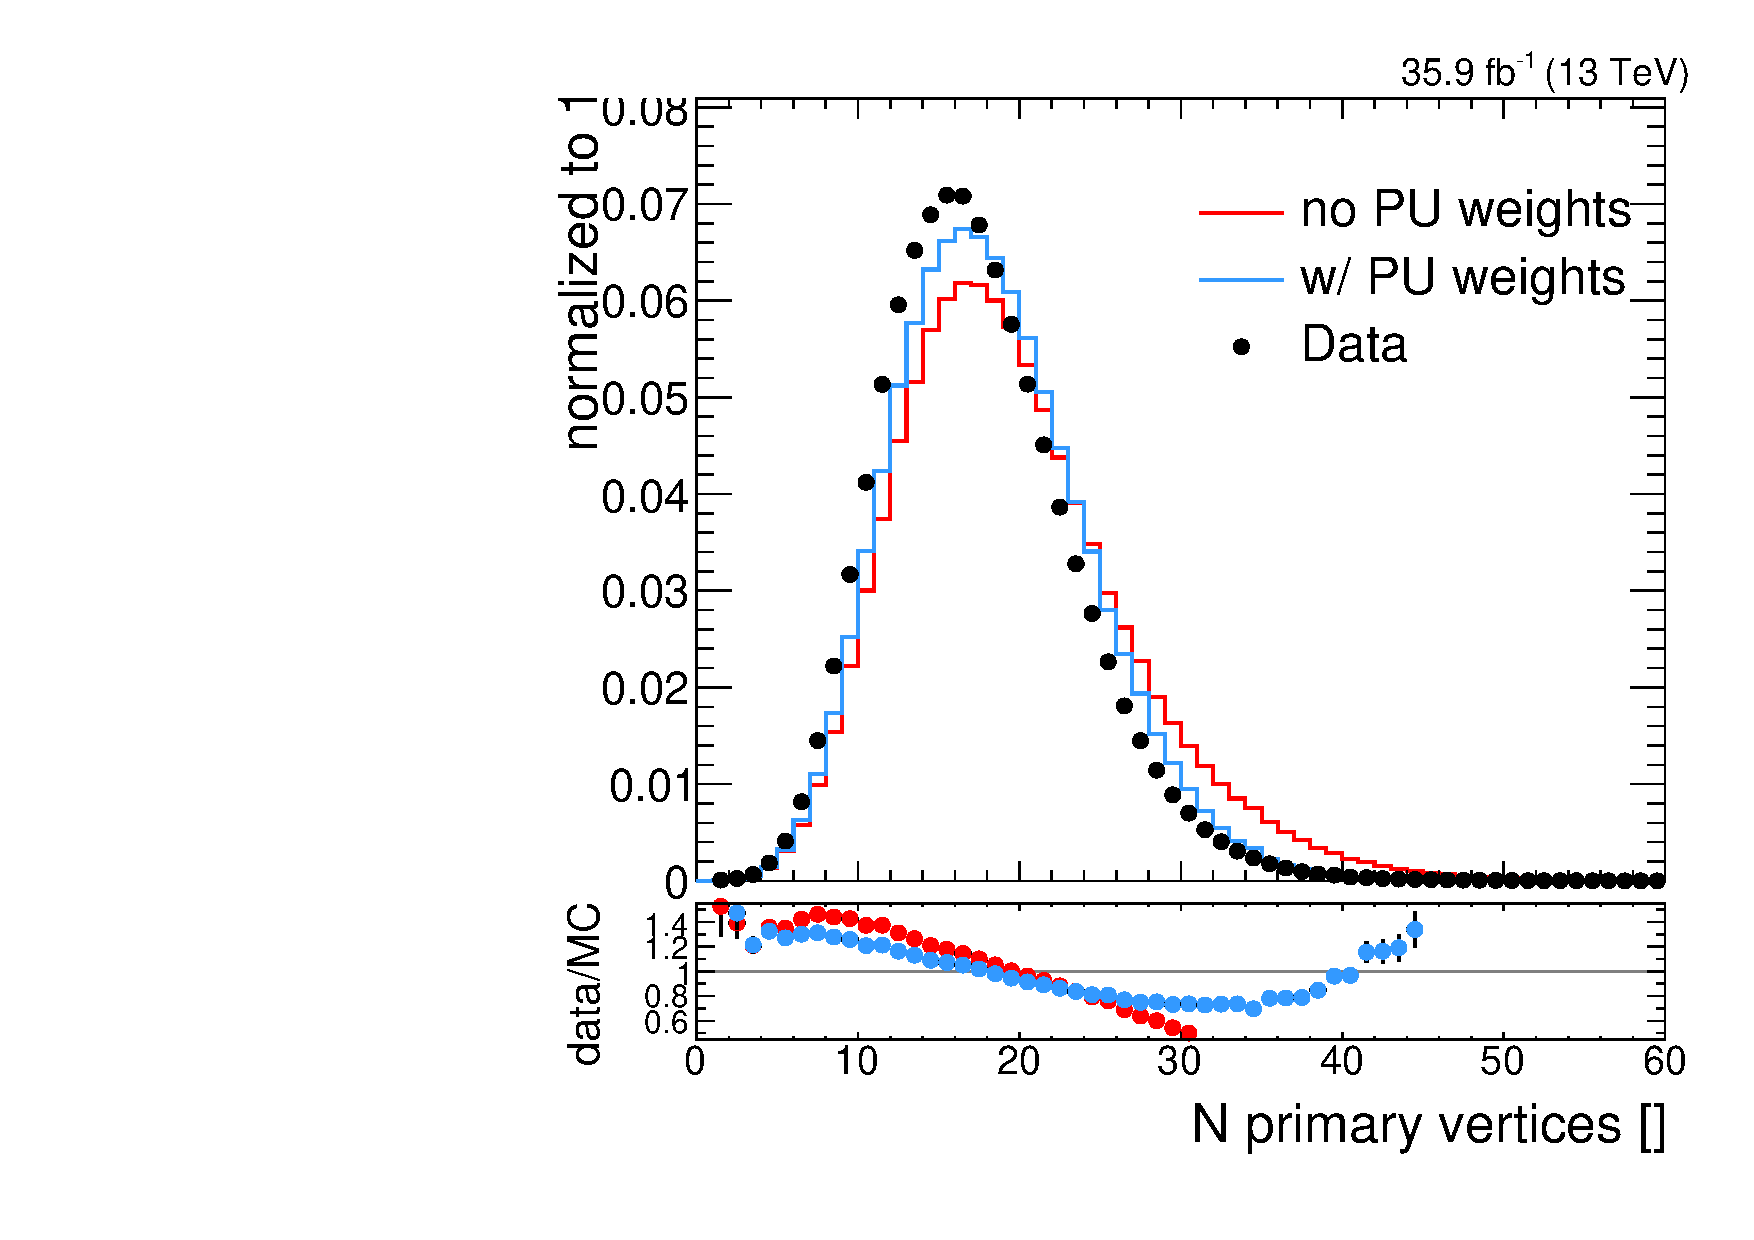
\includegraphics[width=0.45\textwidth]{fig/analysis/PUrewN_0_2016_nVert.pdf}
  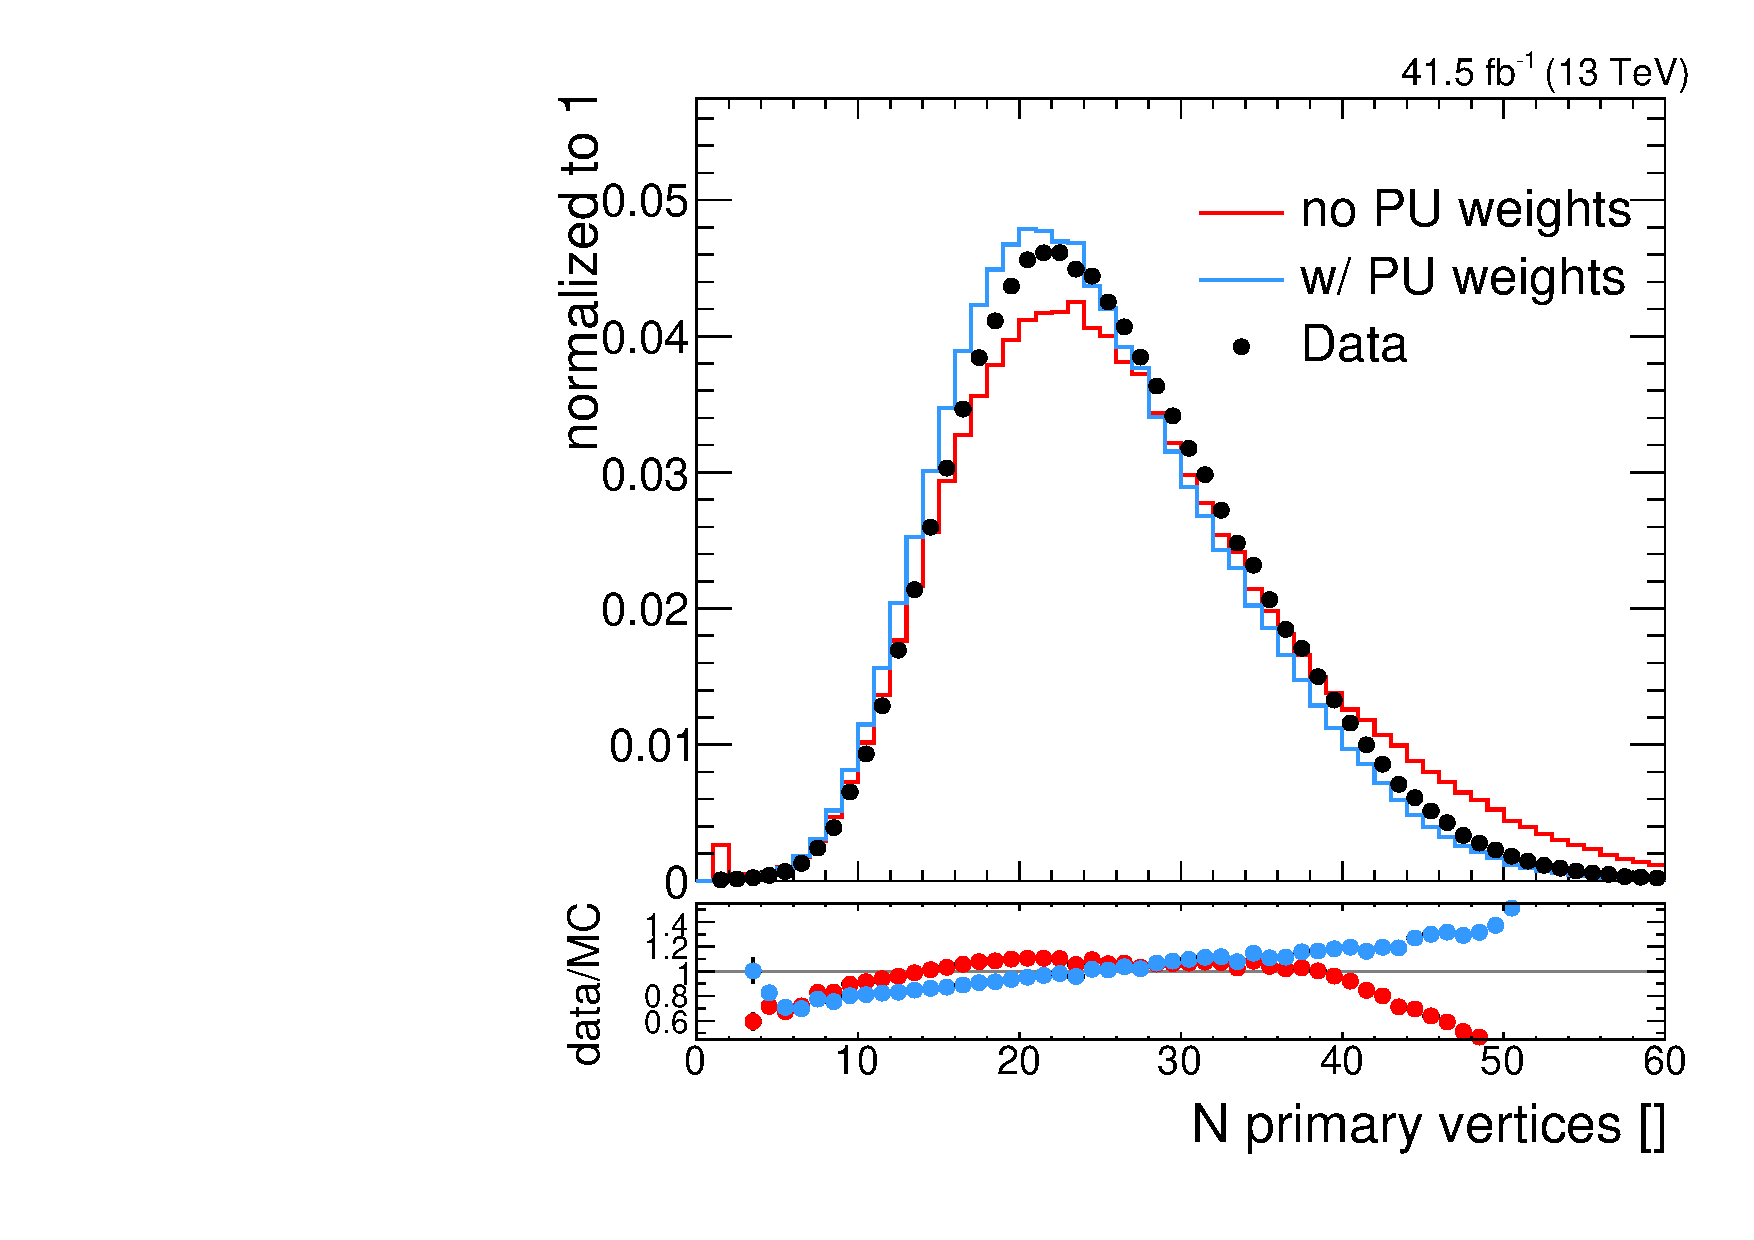
\includegraphics[width=0.45\textwidth]{fig/analysis/PUrewN_0_2017_nVert.pdf}\\
  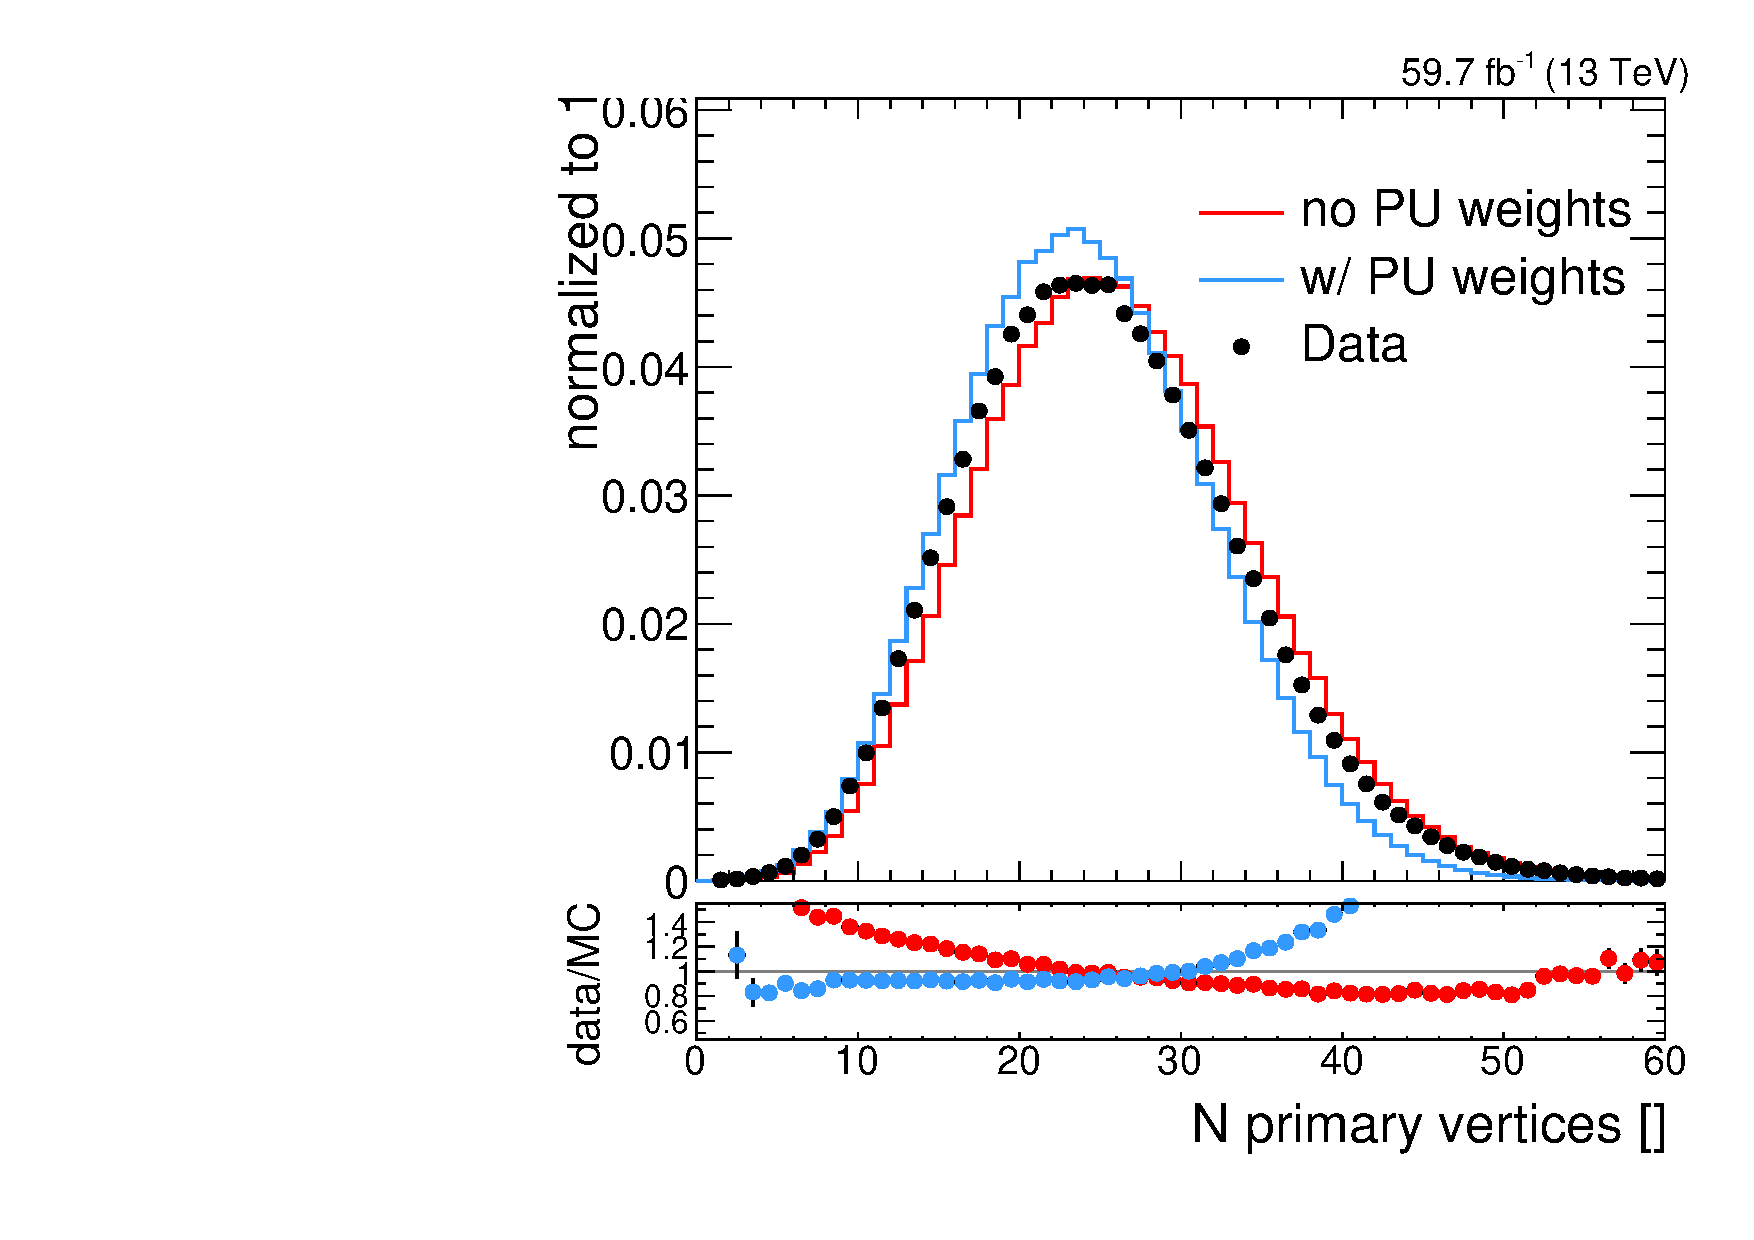
\includegraphics[width=0.45\textwidth]{fig/analysis/PUrewN_0_2018_nVert.pdf}
  \caption{
    Distribution of the number of primary vertices reconstructed in simulation before and after pileup reweighting, with data present, for 2016 (top left), 2017 (top right), and 2018 (bottom).
  }
  \label{fig:PUreweight}
\end{figure}

\subsection{Muon Selection}
\label{subsec:muonSelect}

% High-pT muon selection criteria
When selecting muons for the analysis, they must pass the following high-\pt muon identification criteria as provided by the CMS Muon POG~\cite{MuonSelection}:
\begin{itemize}
  \item The muon is reconstructed as a ``global'' muon.
  \item At least one muon-chamber hit included in the global-muon track fit or in the TuneP fit.
  \item Muon segments in at least two muon stations.
  \item The \pt relative error ($\sigma(\pt)/\pt$) of the muon best track is less than 30\%.
  \item Its tracker track has transverse impact parameter $d_{xy}<2\unit{mm}$ with respect to the primary vertex.
  \item The longitudinal distance of the tracker with respect to the primary vertex is $d_z<5\unit{mm}$.
  \item The muon track has at least one pixel hit.
  \item The muon track has at least six tracker layer hits.
\end{itemize}

% Further muon selection
In addition to the high-\pt muon identification criteria, for this analysis we also require each muon to have $\pt>55\unit{GeV}$ and to be confined to the region $|\eta|<2.4$.
We also apply an isolation requirement on the muons in order to further suppress background.
This is done using the full relative particle flow isolation using $\Delta\beta$ corrections, with the requirement that $I_\mathrm{rel}<0.05$.

Scale factors for muon ID as provided by the Muon POG are also applied~\cite{MuonPAGs}.
To appropriately apply these scale factors as they vary by year to the full Run 2 data set, we weight them by the fraction of integrated luminosity for each year.
We also apply a scale factor for the isolation requirement, which is shown in figure~\ref{fig:muonIsoSF}.
This scale factor was derived on top of muon high-\pt ID, in boosted $Z$ and DY events over the full Run 2 period, which is found to be within 1\% from unity and smaller than the systematic uncertainty for the muon trigger/reco/ID of 5\% used in signal extraction.

\begin{figure}[htbp]
  \centering
  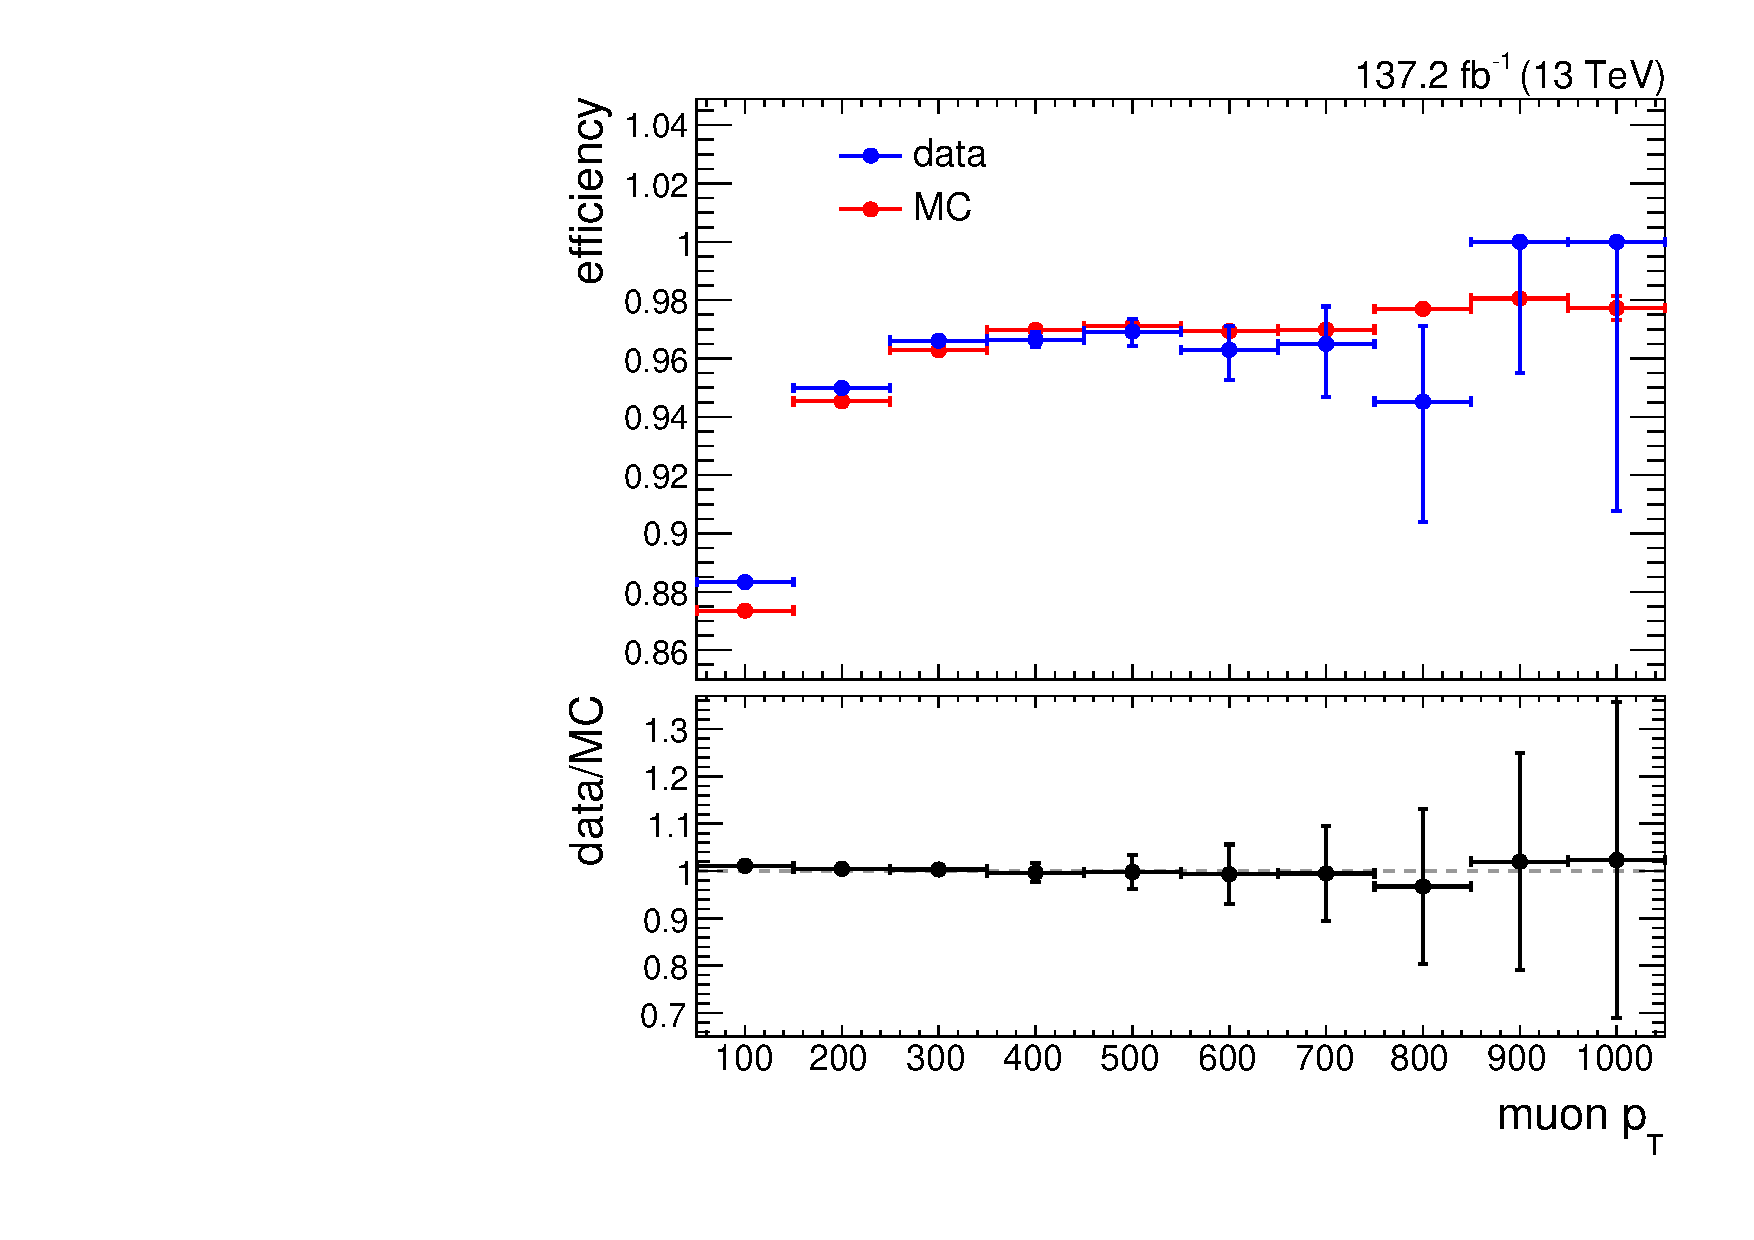
\includegraphics[width=0.65\textwidth]{fig/analysis/muonFullIsoSF.pdf}
  \caption{
    Efficiency in data and simulation and data/MC scale factor for muon isolation requirement.
  }
  \label{fig:muonIsoSF}
\end{figure}

\subsection{Electron Selection}
\label{subsec:elecSelect}

% Electron reconstruction
The electrons that are reconstructed from trigger primitives in the ECAL are required to pass the ``HEEP v7.0'' ID requirements as prescribed by the E/Gamma POG~\cite{HEEPV70}.
The ID requirements ensure that the reconstructed electrons from the ECAL energy deposits are paired with a high quality track from the inner tracker and have a shape consistent with an electromagnetic shower in the calorimeter.
These requirements are listed in table~\ref{tab:HEEPV70}.
For our analysis, we also require them to have $\pt>55\unit{GeV}$ and be within the pseudorapidity range $|\eta|<2.5$, except for the region $[1.4442,1.566]$. % Unsure why this range is excluded
We also apply scale factors for the HEEP ID requirements along with RECO scale factors as recommended by the E/Gamma POG~\cite{EgammaScale}.

\begin{table}[htbp]
  \centering
  % !TEX root = ../../thesis.tex
\footnotesize
\begin{tabular}{lll}
  \hline
  Variable                          & Barrel                             & Endcap                             \\
  \hline
  \multicolumn{3}{c}{Acceptance selections}\\
  \Et                               & $\Et>35\unit{GeV}$                 & $\Et>35\unit{GeV}$                 \\
  $\eta$                            & $|\eta_{SC}|<1.4442$               & $1.566<|\eta_{SC}|<2.5$            \\
  \multicolumn{3}{c}{Identification selections}\\
  \texttt{isEcalDriven}             & \texttt{true}                      & \texttt{true}                      \\
  $\Delta\eta_\mathrm{in}^\mathrm{seed}$          & $|\Delta\eta_\mathrm{in}^\mathrm{seed}|<0.004$ & $|\Delta\eta_\mathrm{in}^\mathrm{seed}|<0.006$ \\
  $\Delta\phi_\mathrm{in}$                 & $|\Delta\phi_\mathrm{in}|<0.06$         & $|\Delta\phi_\mathrm{in}|<0.06$         \\
  $H/E$                             & $H/E<1/E+0.05$                 & $H/E<5/E+0.05$                 \\
  $\sigma_{i\eta i\eta}$            & -                                  & $\sigma_{i\eta i\eta}<0.03$      \\
  $\frac{E_{1\times5}}{E_{5\times5}}$, $\frac{E_{2\times5}}{E_{5\times5}}$        & $\frac{E_{1\times5}}{E_{5\times5}}>0.83$ or $\frac{E_{2\times5}}{E_{5\times5}}>0.94$ & -                              \\
  Inner lost layer hits             & lost hits $\leq1$                  & lost hits $\leq1$                  \\
  Impact parameter, $d_{xy}$        & $|d_{xy}|<0.02$                    & $|d_{xy}|<0.05$                    \\
  \multicolumn{3}{c}{Isolation selections}\\
  EM + had depth 1                  & $iso<2+0.03\Et+0.28\rho$     & $iso<2.5+0.28\rho$ ($\Et<50\unit{GeV}$) \\
  isolation, $iso$                  &                                    & else $iso<2.5+0.03(\Et-50\unit{GeV})+0.28\rho$ \\
  $\pt$ isolation, $isopt$          & $isopt<5\unit{GeV}$                   & $isopt<5\unit{GeV}$                   \\
  \hline
\end{tabular}

  \caption{
    Definitions of HEEP ID V7.0 selections.
  }
  \label{tab:HEEPV70}
\end{table}

\subsection{Jet Selection}
\label{subsec:jetSelect}

% Types of jets
As mentioned previously, there are two types of jets that are expected to be produced in the signal events of interest.
The first is a large-radius jet that is produced via the \VorH decay that exhibits two-pronged substructure, while the second type are small-radius forward-facing jets only present in \VBF production modes.
This analysis therefore categorizes candidate jets into the two following types:
\begin{itemize}
  \item ``Large-radius'' AK8 jets: \VorH boson candidates that decay into $q\bar{q}^{(\prime)}$ or $b\bar{b}$, using the anti-\kt algorithm with distance parameter $R=0.8$.
  \item ``Standard'' AK4 jets: \VBF forward jet candidates, using the anti-\kt algorithm with distance parameter $R=0.4$.
\end{itemize}

% The anti-kt algorithm
The anti-\kt algorithm is a jet clustering algorithm reconstructs jets by introducing distances $d_{ij}$ between objects $i$ and $j$ and $d_{i,B}$ between object $i$ and the beam $B$~\cite{Cacciari_2008}.
The algorithm starts by assigning values for $d_{ij}$ and $d_{i,B}$ for all objects in the final state, and finds the minimum value among the distances.
If the minimum value is a $d_{i,B}$ value, then object $i$ is declared to be a jet and removed from the list, and the algorithm starts over from the first step.
If instead it is a $d_{ij}$ value, then objects $i$ and $j$ are combined and the algorithm goes back to the first step.
This process is repeated until all particles have been declared jets, with $d_{ij}$ and $d_{i,B}$ defined by
\begin{align}
  d_{ij} &= \min\pqty{k_{\mathrm{T},i}^{2p},k_{\mathrm{T},j}^{2p}}\frac{\Delta_{ij}^2}{R^2},\\
  d_{i,B} &= k_{\mathrm{T},i}^{2p},
\end{align}
where $\Delta_{ij}^2=(y_i-y_j)^2+(\phi_i-\phi_j)^2$, with $k_{T,i}$ as the transverse momentum for object $i$, $y_i$ the rapidity for object $i$, $\phi_i$ is the azimuthual angle for object $i$, $R$ is the distance parameter for the algorithm, and $p$ is a parameter determined by the jet clustering algorithm.
For the anti-\kt algorithm, $p=-1$, with other algorithms taking on different values, such as $p=1$ for the \kt algorithm~\cite{Marzani_2019}.

% Jet selection
For both types of jets, we use tight ID jets as recommended by the JetMET POG~\cite{jetID2016,jetID2017,jetID2018}.
We also apply jet energy corrections for data and MC prescribed by the Jet Energy Resolution and Corrections (JERC) subgroup~\cite{JetEnergyScale}.
The hadronic jet resulting from the \VorH decay is selected by taking the jet with the highest \pt from the large-radius jets, with a minimum threshold of $\pt>200\unit{GeV}$ and a pseudorapidity range of $|\eta|<2.4$.
Any large-radius jets that have an electron or tight muon within $\Delta R=\sqrt{\Delta\eta^2+\Delta\phi^2}<1.0$ are discarded to suppress background events.
For the standard jets, we require that $\pt>30\unit{GeV}$, and we discard any jets within $\Delta R<0.4$ of any tight electron or tight muon, or within $\Delta R<0.8$ of any large-radius jet.

\subsubsection{$V$-jet Tagging}

% V-jet identification
A central component of the analysis is the ability to accurately identify and reconstruct the hadronically decaying \VorH boson, which we shall refer to as \Vhad.
Once the jets in the final state are identified, algorithms must be applied to determine the substructure of the jets.
This analysis makes use of the Pileup Per Particle Identification (PUPPI) algorithm, which takes particle flow object candidates and assigns weights to each particle based energy shape profiles~\cite{Bertolini_2014}.
The resulting reweighted candidates are then put into substructure algorithms for further analysis.

% Jet grooming
The jets obtained from the PUPPI algorithm are then groomed by using the ``soft drop'' algorithm~\cite{Larkoski_2014}, which removes soft wide-angle radiation from jets.
For a jet with radius $R$ with two constituents, the soft drop algorithm removes the softer constituent if it does not satisfy the condition
\begin{equation}
  \frac{\min\pqty{p_{\mathrm{T},1},p_{\mathrm{T},2}}}{p_{\mathrm{T},1}+p_{\mathrm{T},2}}>z\pqty{\frac{\Delta R_{12}}{R}}^\beta,
\end{equation}
where the $p_{\mathrm{T},i}$ are the transverse momenta of the jet constituents, $\Delta R_{12}$ is the separation between the constituents in the $y$-$\phi$ plane, $R$ is the radius of the jet, $z$ is the soft drop threshold, and $\beta$ is the angular exponent.
For this analysis, we use $z=0.1$ based on theoretical considerations of the jet mass from QCD~\cite{Dasgupta_2013,Dasgupta_2013_2}.
We denote the soft drop mass by \MJ, and apply corrections as recommended by JetMET POG~\cite{WZ-tagging}.

% N-subjettiness
To determine the degree to which the jet has substructure, we use the ``$N$-subjettiness'' as a measure of how many subjets are present in the jet~\cite{Thaler_2011,Thaler_2012}.
It is designed to identify boosted hadronic objects based on the angular distances of jet constituents relative to their nearest subjet axis.
Figure~\ref{fig:jetSubstruct} shows an example of a jet with two subjects defined by axes $\mathbf{\hat{n}}_1$ and $\mathbf{\hat{n}}_2$, which is the two-pronged structure expected to be observed by the \Vhad boson decay.
We proceed by reclustering the jets with the \kt algorithm until $N$ jets remain, then compute the $N$-subjettiness defined by
\begin{equation}
  \tau_N=\frac{1}{d_0}\sum_kp_{\mathrm{T},k}\min\pqty{\Delta R_{1,k},\Delta R_{2,k},\ldots,\Delta R_{N,k}},
\end{equation}
where $d_0$ is a normalization factor given by
\begin{equation}
  d_0=\sum_kp_{\mathrm{T},k}R_0,
\end{equation}
with $R_0$ as the clustering parameter of the original jet, $p_{\mathrm{T},k}$ is the transverse momentum of the $k$-th jet constituent, and $\Delta R_{n,k}$ is the distance to the $n$-th subject in the $\eta$-$\phi$ plane.

\begin{figure}[htbp]
  \centering
  % !TEX root = ../../thesis.tex
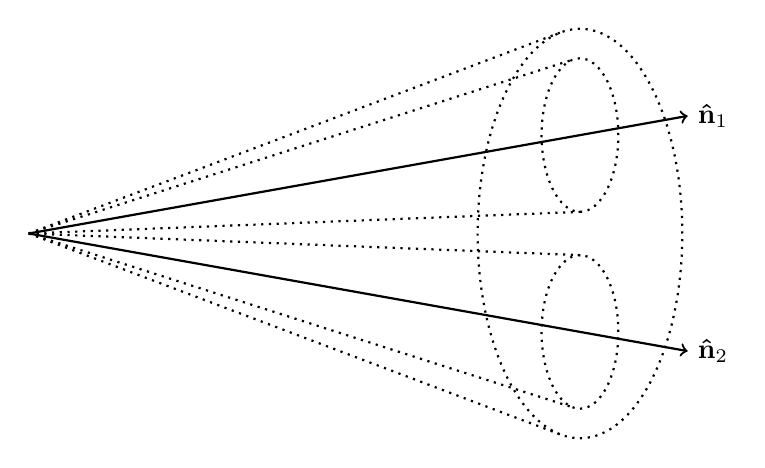
\begin{tikzpicture}
  % Main jet
  \draw[rotate around={270:(0,0)},dotted,thick] (0,7) ellipse (2.6 and 1.3);
  \draw[rotate around={270:(0,0)},dotted,thick] (0,0) -- (69.29:7.21);
  \draw[rotate around={270:(0,0)},dotted,thick] (0,0) -- (110.71:7.21);

  % Subjets
  \draw[rotate around={270:(0,0)},dotted,thick] (1.25,7) ellipse (0.975 and 0.4875);
  \draw[rotate around={270:(0,0)},dotted,thick] (0,0) -- (72.275:7.26);
  \draw[rotate around={270:(0,0)},dotted,thick] (0,0) -- (87.75:7.01);
  \draw[rotate around={270:(0,0)},dotted,thick] (-1.25,7) ellipse (0.975 and 0.4875);
  \draw[rotate around={270:(0,0)},dotted,thick] (0,0) -- (92.25:7.01);
  \draw[rotate around={270:(0,0)},dotted,thick] (0,0) -- (107.725:7.26);

  % Axes
  \draw[->,thick] (0,0) -- (10.12:8.5) node[right] {$\mathbf{\hat{n}}_1$};
  \draw[->,thick] (0,0) -- (-10.12:8.5) node[right] {$\mathbf{\hat{n}}_2$};
\end{tikzpicture}

  \caption{
    Illustration of jet substructure for a two-pronged jet with axes $\mathbf{\hat{n}}_1$ and $\mathbf{\hat{n}}_2$.
    The $N$-subjettiness $\tau_N$ is used as a measure of how many subjets are present within a jet.
  }
  \label{fig:jetSubstruct}
\end{figure}

% N-subjettiness ratios
In some cases it is advantageous to consider ratios of $N$-subjettiness.
For example, in this analysis we consider the ratio $\tau_2/\tau_1=\nsubj$, which is a measure of whether or not the jet exhibits the properties we would expect from a jet with 2 subjets versus a single jet with no substructure.
This allows for separating jets originating from boosted vector bosons versus jets that are produced from quarks and gluons, thereby allowing further background suppression.
This analysis uses a modified version of the $N$-subjettiness ratio that reduces the dependency of \nsubj on the jet mass, which is denoted by the designed decorrelated tagger (DDT) $N$-subjettiness \nsubjDDT~\cite{Dolen_2016}.
It is defined by
\begin{equation}
  \nsubjDDT=\nsubj-C\ln\pqty{\frac{\MJ^2}{\ptjet\times(1\unit{GeV})}},
\end{equation}
where $C$ is a coefficient obtained by taking the slope of a fit for the \nsubj profile versus $\ln\pqty{\frac{\MJ^2}{\ptjet\times(1\unit{GeV})}}$ in non-resonant \Wjets background events after applying the full analysis selection cuts.

% N-subjettiness selection
For this analysis, we only consider large-radius jets that satisfy $\nsubjDDT<0.80$.
We also later use \nsubjDDT for event categorization to split the analysis into high and low purity jet categories.

\subsubsection{$b$-tagging}

% CHS approach
While the boosted jets resulting from the \Vhad decay are identified and groomed using algorithms such as the anti-\kt and PUPPI algorithms, the candidate four vector for the $X$ boson is estimated using jet energy scale corrections and charged hadron subtraction (CHS).
The CHS approach is used in order to suppress background contribution from top quark production, which results in the production of jets from $b$ decays.

% b-tagging details
Jets in the region $|\eta|<2.4$ are $b$-tagged if they pass the \texttt{medium} working point of the Combined Secondary Vertex (CSV) or DeepCSV algorithms, as recommended by the $b$-tag and vertexing (BTV) POG.
The \texttt{medium} working point for CSV is 0.8484 in 2016~\cite{bTagging2016}, and for DeepCSV the working points are 0.4941 and 0.4184 for 2017 and 2018, respectively~\cite{bTagging2017,bTagging2018}.
We also apply $b$-tagging scale factors and weights that depend on the jet \pt, $\eta$, and value of the $b$-tagging discriminant as prescribed by the BTV POG~\cite{bTaggingEff,bTaggingSF}.

\subsubsection{$H(b\bar{b})$-tagging}

% The need for bb-tagging
The $V$-tagging methods previously described account for identifying and grooming jets resulting from the $\Vhad$ decay, but additional techniques are applied in this analysis to account for a large-radius \bbbar jet.
Such a jet signifies the decay \Htobbbar in the final state and hence a \WH resonance, which allows for discriminating against background with light jet flavors.
For this reason, we use a $b$-tagging discriminator to identify Higgs boson jet candidates that uses information from displaced tracks and secondary vertices~\cite{CMS-PAS-BTV-15-002}.
We also apply a cut on the M2 operating point of the ``\DoubleB tagger'' to categorize events, for which the threshold is 0.8 for Run 2 according to references~\cite{bTagging2016,bTagging2017,bTagging2018}.

% Scale factors
Additionally, we apply scale data/MC efficiency scale factors to our signal sample normalizations as recommended by the BTV POG, while the scale factors for the background are estimated from the data in the control regions.
We use two sets of scale factors that depend on \ptjet.
One is for \Htobbbar jets resulting from the \WprtoWHtolnubbbar signal model, and the other is for mistagging $W$ bosons resulting from $t\bar{t}$ events, which are applied to the \GBulktoWWtolnuqqbarpr and \WprtoWZtolnuqqbar signal models.
These scale factors are applied from method 1a from reference~\cite{bTaggingEff}.
First we measure the MC $bb$-tagging efficiencies $\epsilon$, then apply the event weights for the \bbbar-tagged category as
\begin{equation}
  w^{\bbbar}(\pt)=\frac{\mathrm{SF}(\pt)\epsilon(\pt)}{\epsilon(\pt)}=\mathrm{SF}(\pt),
\end{equation}
where $\mathrm{SF}$ denotes the scale factors.
For the \bbbar-untagged category, we instead use
\begin{equation}
  w^{\mathrm{no}\bbbar}(\pt)=\frac{1-\mathrm{SF}(\pt)\epsilon(\pt)}{1-\epsilon(\pt)}.
\end{equation}

\subsection{Missing Transverse Energy}

% MET
For this analysis, we use type-I corrected particle flow MET (PFMET) to account for the energy of the neutrino from the \Wlep decay, where PFMET is defined as the magnitude of the negative vector sum of all transverse energies from particle flow objects~\cite{PFMET}.
The correction is a propagation of the jet energy corrections (JEC) to MET, which is given by
\begin{equation}
  \EtmissTI=\vqty{-\sum_\mathrm{jet}\mathbf{p}_\mathrm{T,jet}^\mathrm{JEC}-\sum_{i\in\mathrm{uncl.}}\mathbf{p}_{\mathrm{T},i}},
\end{equation}
where the first sum is over clustered jets and the second sum is over unclustered particles.

\subsection{Leptonic $W$ and \WV reconstruction}

% Leptonic reconstruction
To reconstruct the leptonically decaying $W$ candidate \Wlep, we select the highest \pt lepton in the event and combine it with the \EtmissTI resulting from the neutrino.
We also apply a $W$ mass constraint to estimate the $z$-component of the missing energy.
The resulting \Wlep is then combined with the large-radius \Vhad jet to form a diboson candidate, with mass denoted by \MVV.

\subsection{VBF Forward Jets}
\label{subsec:VBFjets}

% VBF signature
The defining signature of the \VBF production process is the presence of two boosted jets in the forward and backward regions of the detector, along with the decay products in the central region of the detector resulting from the \Wlep and \Vhad resonances.
The analysis therefore requires additional kinematic constraints in order to categorize \VBF-produced events, which take into account properties of the forward-facing \VBF jets such as their combined mass and separation in $\eta$.

% VBF jet selection
We select candidate \VBF jets from the two highest \pt standard AK4 jets as defined in subsection~\ref{subsec:jetSelect}.
This requires that the \VBF jets pass $\pt>30\unit{GeV}$, and that they do not overlap with the selected lepton and large-radius jet.
We then apply selection cuts to the two candidate \VBF jets based on their separation in pseudorapidity \DetaVBF and \VBF dijet mass \mjjVBF.

% VBF Deta selection cut
For the cut on \DetaVBF, we exploit the fact that the \VBF jets are expected to be found in the high $|\eta|$ regions of the detector near the endcaps and be roughly anti-parallel to each other.
Figure~\ref{fig:detaSB_VBF} (left) shows the relative shape differences in \DetaVBF between the \VBF\RadtoWW signal MC sample and the background MC samples used in this analysis.
To retain a signal efficiency of 40-50\%, we choose a cut of $\DetaVBF>4$.

\begin{figure}[htbp]
  \centering
  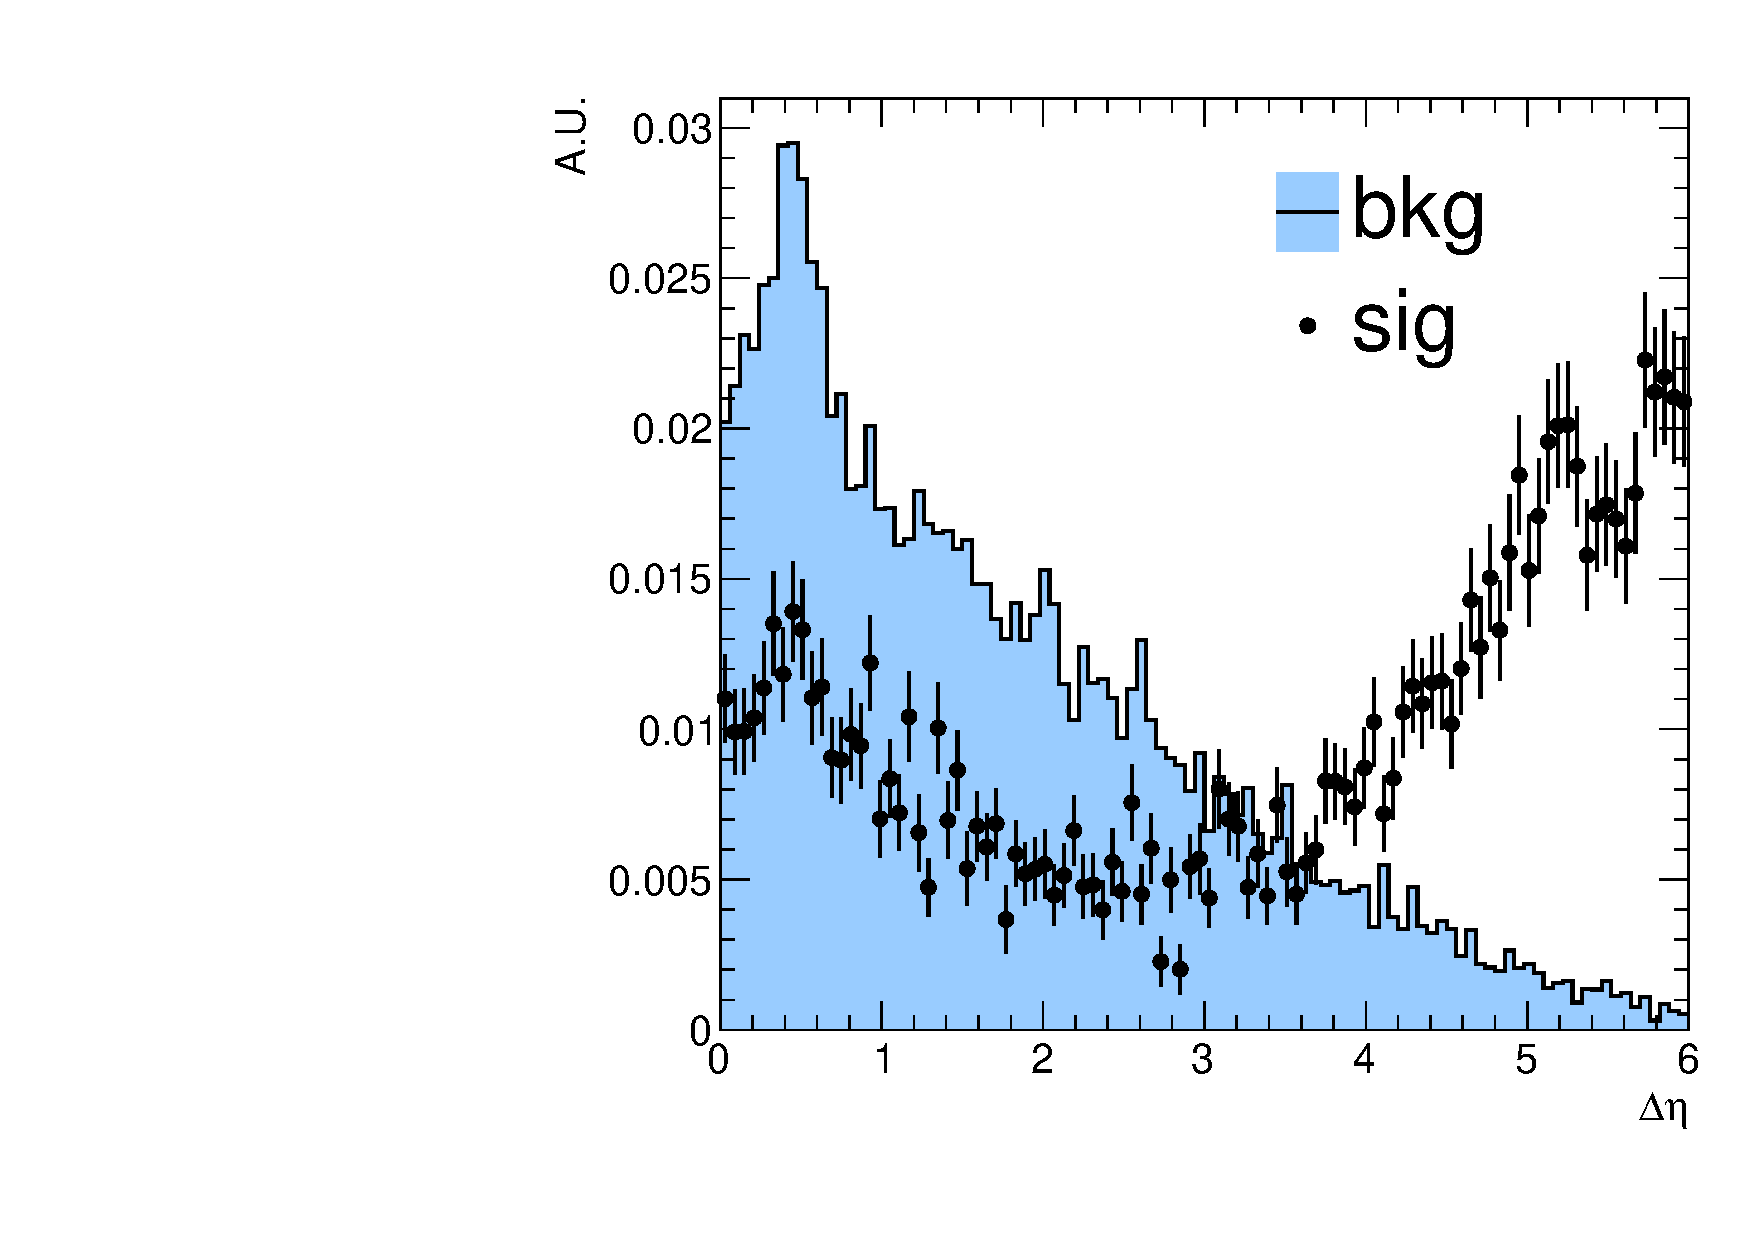
\includegraphics[width=0.45\textwidth]{fig/analysis/detaSB.pdf}
  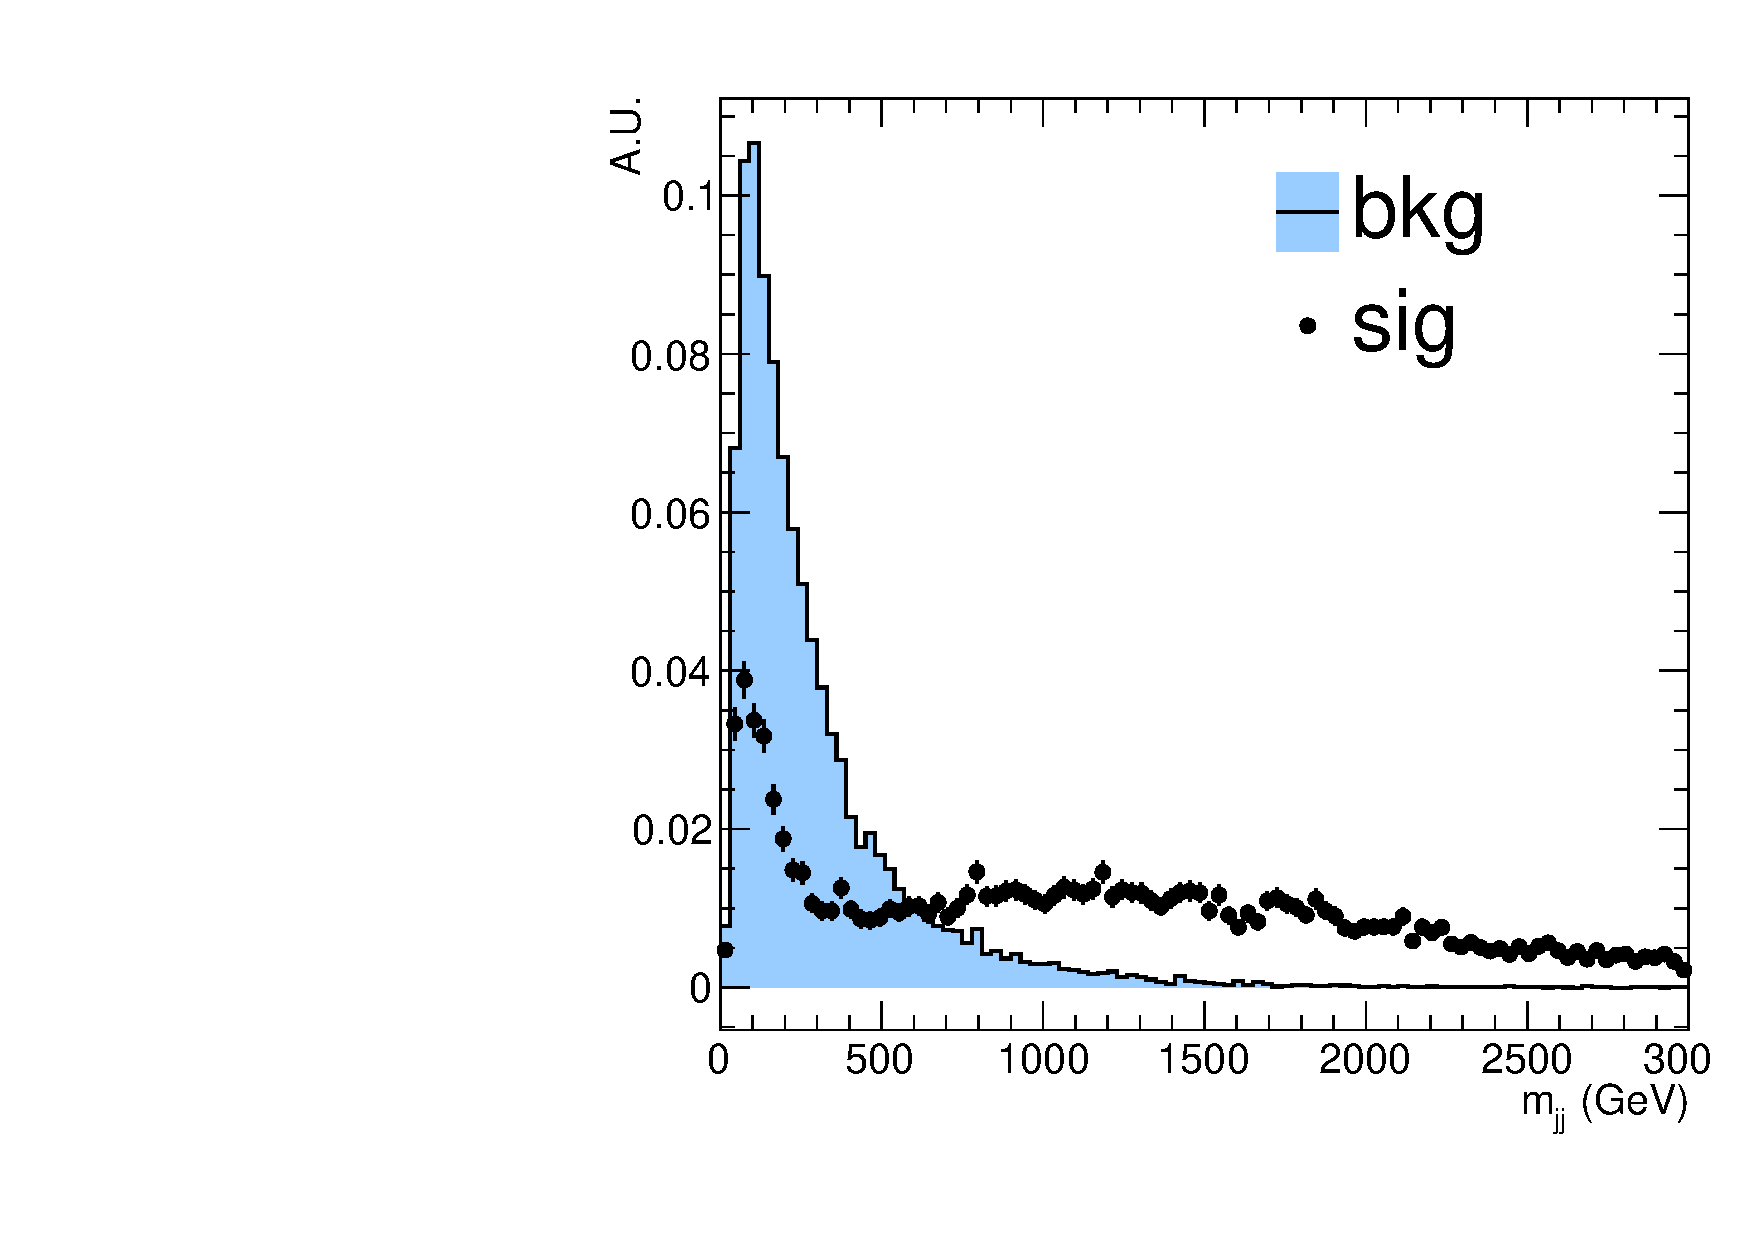
\includegraphics[width=0.45\textwidth]{fig/analysis/mjjSB.pdf}\\
  \caption{
    Shape comparison of a \VBF\RadtoWW signal sample and background MC samples, normalized to unity, for \DetaVBF (left) and \mjjVBF (right).
    The shape discrepancy between the \VBF signal and background distributions in \DetaVBF and \mjjVBF allows for distinguishing signal from background.
  }
  \label{fig:detaSB_VBF}
\end{figure}

% VBF dijet mass selection cut
The other kinematic cut applied to the \VBF candidate jets is on the invariant mass of the sum of the \VBF jet four vectors, \mjjVBF.
For this cut, we consider the Punzi significance obtained for a \VBF signal sample as a function of the thresholds of the cuts for \DetaVBF and \mjjVBF.
The Punzi significance is defined by $\epsilon/(1.5+\sqrt{B})$, where $\epsilon$ is the number of signal events obtained by the cuts assuming an integrated luminosity of $\mathcal{L}_\mathrm{int}=1\unit{pb^{-1}}$ and a cross section of $\sigma=1\unit{pb}$, while the number of background events $B$ is weighted with the total luminosity~\cite{Punzi:2003bu}.
Figure~\ref{fig:detaMjjSB_VBF} shows the Punzi significance for the \VBF\RadtoWW signal sample in the plane spanned by the thresholds for the \DetaVBF and \mjjVBF cuts.
We again require that the selection cut on \mjjVBF retains 40-50\% signal efficiency, as we did for \DetaVBF.
This leads to a cut of $\mjjVBF>500\unit{GeV}$.

\begin{figure}[htbp]
  \centering
  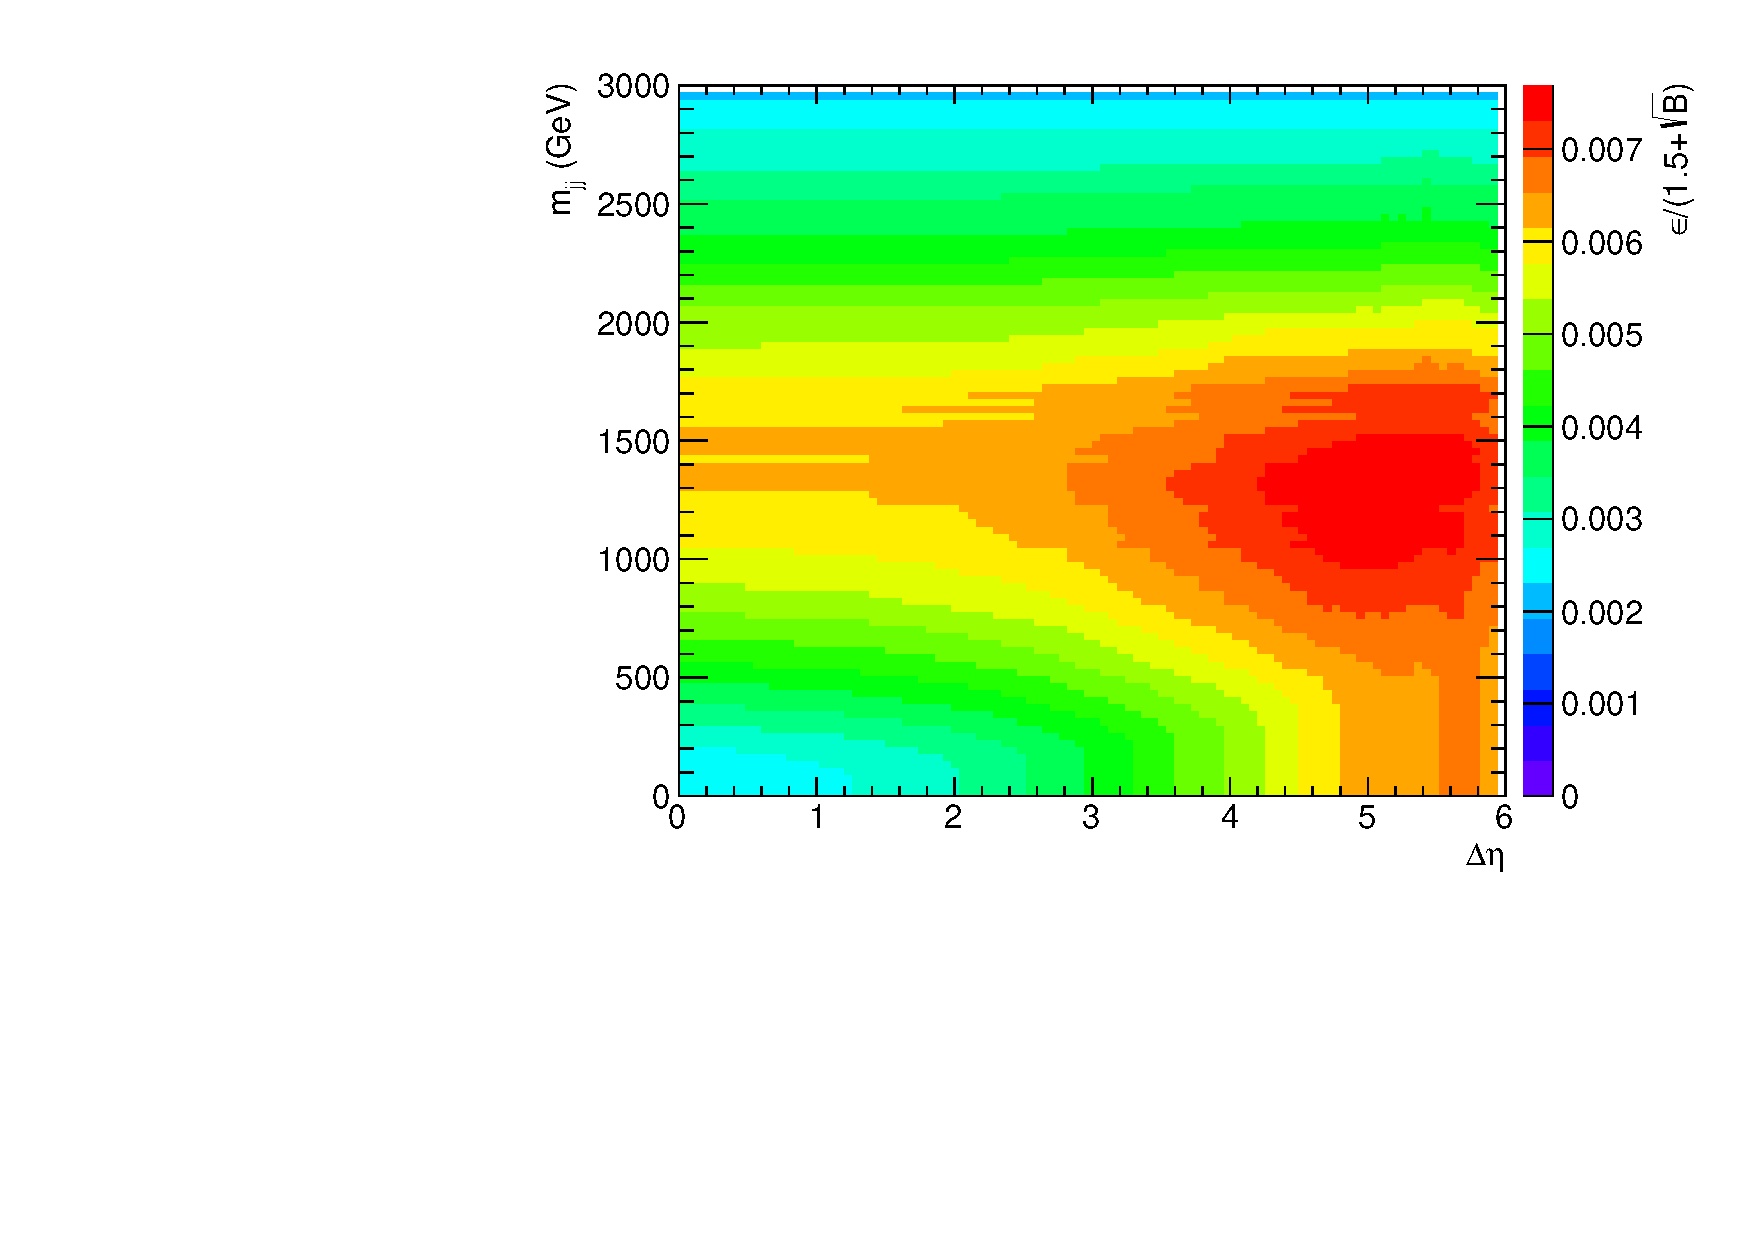
\includegraphics[width=0.5\textwidth]{fig/analysis/detaMjjSB.pdf}
  \caption{
    Two-dimensional Punzi significance of the \VBF\RadtoWW signal in the plane of the two thresholds of the cuts on \DetaVBF and \mjjVBF.
  }
  \label{fig:detaMjjSB_VBF}
\end{figure}

\subsection{Spin Polarization and Boson Rapidities}
\label{subsec:spinPol}

% Spin polarization from VBF production
The \VBF production process has another distinctive feature in which some kinematic variables are sensitive to the spin of the $X$ resonance, thereby providing the ability to distinguish between signal models.
This effect can be seen in the distributions for the separation in rapidity between the \Vhad and \Wlep diboson system, which we denote by \Dy.
Figure~\ref{fig:DyComp} shows the shape discrepancies between the MC signals and backgrounds in \Dy, separated by non-\VBF (left) and \VBF-produced signals.

\begin{figure}[htbp]
  \centering
  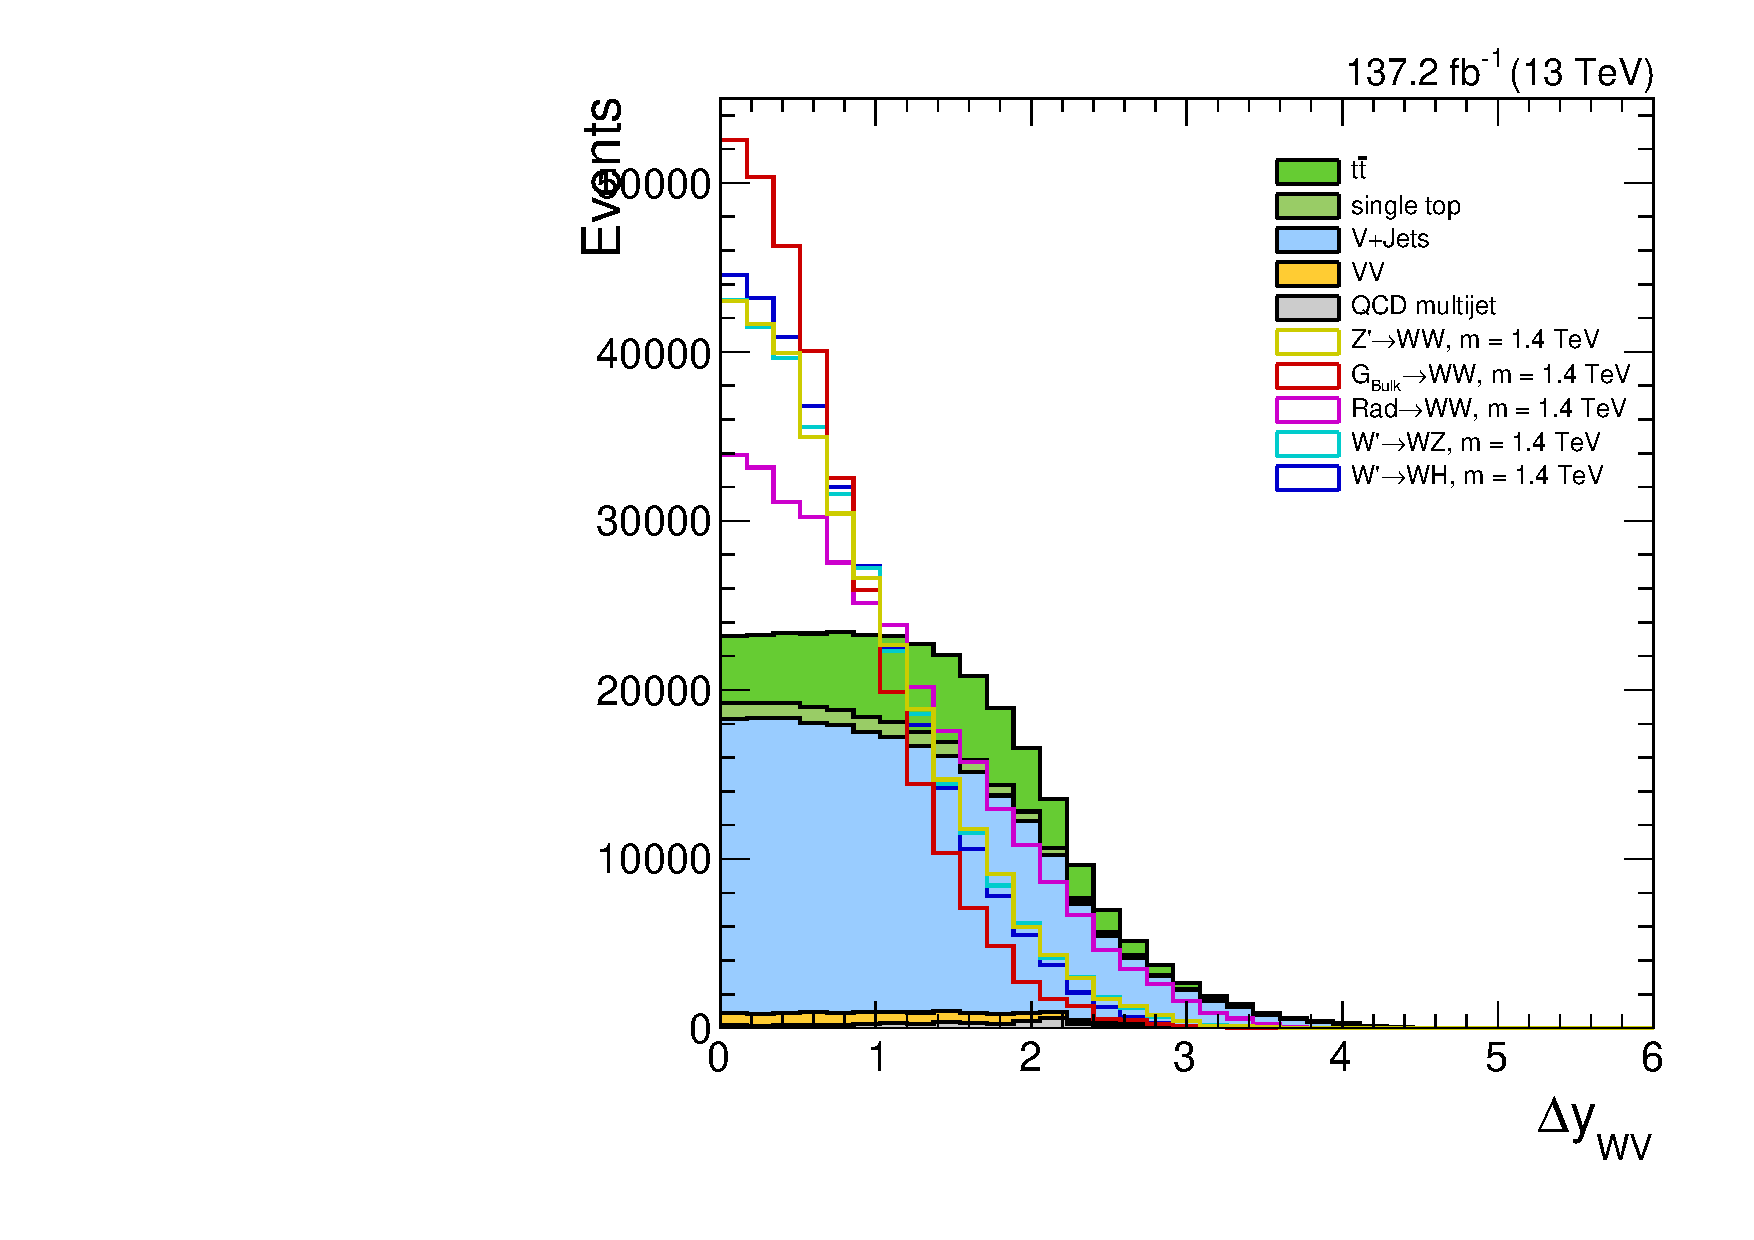
\includegraphics[width=0.45\textwidth]{fig/analysis/SR_b1_allL_allP_allC_inc_lo_Run2_Dy.pdf}
  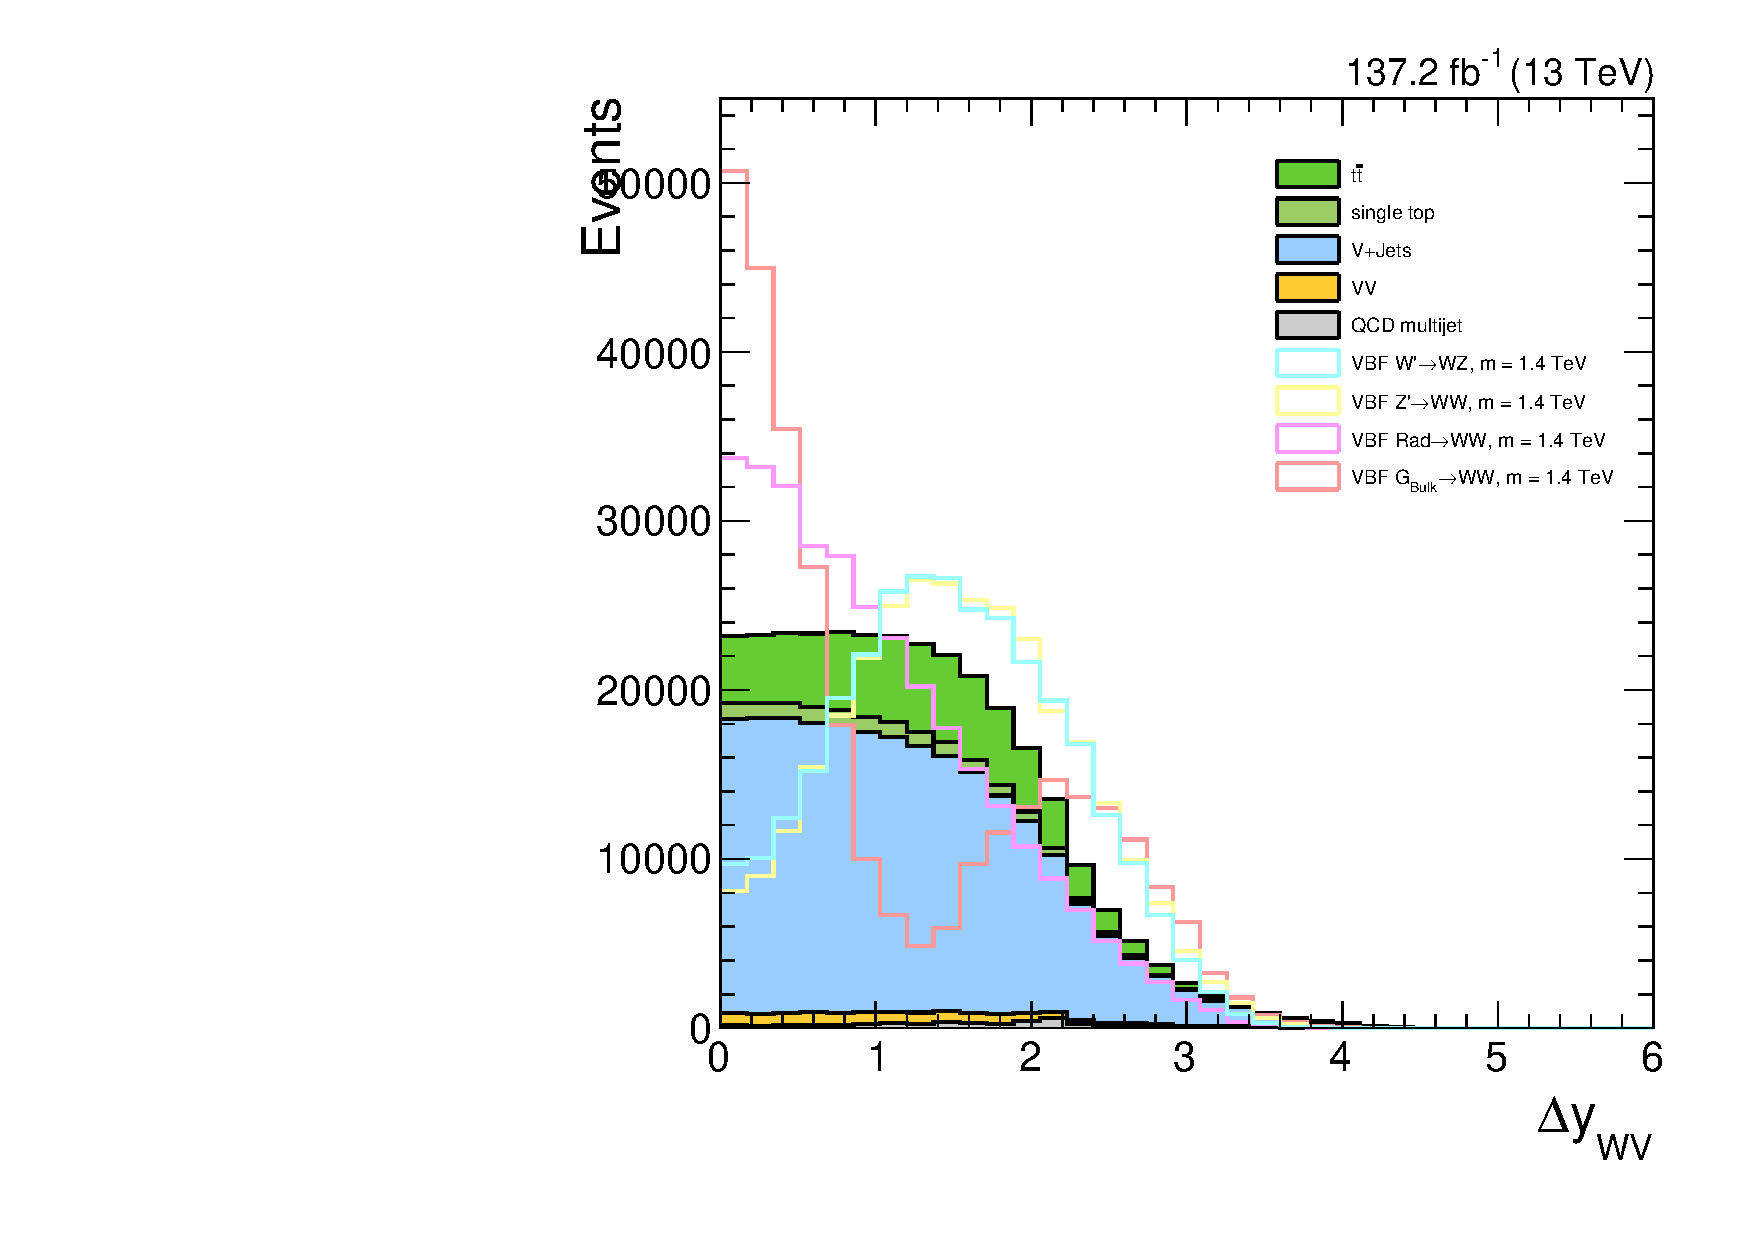
\includegraphics[width=0.45\textwidth]{fig/analysis/SR_b1_allL_allP_allC_vbf_lo_Run2_Dy.pdf}\\
  \caption{
    Shape comparison of the angular separation \Dy between the two reconstructed bosons for simulated background and signals, in the signal region.
    Backgrounds distributions are stacked and normalized to the expected luminosity for the full Run-2, while signal distributions are overlaid, all arbitrarily normalized to the same integral as the sum of backgrounds.
    Non-\VBF (left) and \VBF (right) signals are shown separately.
    The shape differences between signals is most apparent in the case of \VBF production, allowing for distinguishing between spin-0, spin-1, and spin-2 signals.
    This defines a new layer of categorization for the analysis.
  }
  \label{fig:DyComp}
\end{figure}

% Non-VBF signals
The signals produced via \ggF or \DY have minor shape differences between each other, and their distributions are consistently narrower and more concentrated in the low \Dy region compared to the background MC samples.
This on its own suggests that categorizing the search based on \Dy would increase the search sensitivity.

% VBF signals
For the \VBF-produced signals, the shape differences between signals are much more apparent.
The spin-1 \VBF\WprtoWZ and \ZprtoWW signals both peak around $\Dy=1.4$ rather than plateauing like the background from $\Dy=0$ to 0.8.
Meanwhile, the spin-2 \VBF\GBulktoWW signal has two peaks, with a large and narrow peak occurring at $\Dy=0$, followed by a smaller peak around $\Dy=2.0$.
Finally, the \VBF\RadtoWW signal exhibits no difference in its \Dy distribution compared to the \ggF\RadtoWW signal since it is a spin-0 resonance, but it still differs from the other \VBF signals since it only has a peak at $\Dy=0$.

% Statistical power of Dy categories
The shape differences between the \VBF signals allow for not only enhancing the search sensitivity by using categories based on \Dy, but by also allowing for distinguishing between spin-0 (\RadtoWW), spin-1 (\ZprtoWW, \WprtoWZ, \WprtoWH), or spin-2 (\GBulktoWW) \VBF signal models.
For this reason, we use two categories based on rapidity: a low-\Dy category defined by the condition $\Dy<1.0$, and a high-\Dy category defined by $\Dy\geq1.0$.
Originally a 3-category scheme was considered for the analysis, but it was found that this did not leave sufficient background MC statistics in all three categories in order to build robust 2D background templates.

\subsection{Final Event Selection and Categorization}
\label{subsec:eventSelect}

% Event selection and categorization
For this analysis, we made a final event selection in order to select events that exhibit the expected behavior of the final state described in subsection~\ref{subsec:expEvent} and optimize the search potential for a semileptonically decaying heavy $X$ resonance produced via \ggF, \DY, or \VBF.
We then divide the analysis into disjoint categories in order to enhance the search sensitivity.

\subsubsection{Final Event Selection}

% Final event selection
The final event selection used in the analysis is defined by the following:
\begin{enumerate}
  \item Exactly one charged lepton as defined in subsections~\ref{subsec:muonSelect} and \ref{subsec:elecSelect}.
  \item Lepton veto: no additional loose electron ($\pt>35\unit{GeV}$) or muon ($\pt>20\unit{GeV}$) in the event.
  \item Type-I corrected missing transverse energy \EtmissTI: events are required to have $\Etmiss>80\unit{GeV}$ for the electron channel and $\Etmiss>40\unit{GeV}$ for the muon channel to suppress contributions from QCD multijet backgrounds.
  \item Leptonic $W$ \pt: the \pt of the reconstructed \Wlep must satisfy $\pt>200\unit{GeV}$ in order to select a boosted $W$ topology.
  \item Hadronic \VorH \pt: the \pt of the reconstructed \Vhad must satisfy $\pt>200\unit{GeV}$ in order to select a boosted \VorH topology.
  \item $b$-tag veto: the event is required to have no $b$-tagged standard jets.
  \item \ZH veto: to ensure that the selection is disjoint from the $X\to\ZH\to\ell\ell\bbbar$ search~\cite{CMS_AN2019_107}, which uses a different electron and muon ID, we explicitly veto events where a \ZH candidate is selected with their criteria.
  \item Search region: the search region is defined as $0.6<\MVV<5.0\unit{TeV}$ and $20<\MJ<210\unit{GeV}$.
\end{enumerate}

\subsubsection{Final Event Categories}
\label{subsec:eventCat}

% Final event categories
After considering the final event selection, we split the analysis into 24 disjoint event categories.
The categories are based on four successive criteria based on the lepton channel, large-radius jet purity, \VBF/non-\VBF categories, and \Dy categories.

% Lepton channel
First, we split the event sample based on the lepton flavor of the reconstructed \Wlep candidate, defining two channels:
\begin{itemize}
  \item {\bfseries Electron channel ($e$)}
  \item {\bfseries Muon channel ($\mu$)}
\end{itemize}

% Jet purity
Second, we exploit the fact that the jets originating from \VorH decays exhibit a two-pronged structure.
The analysis is split based on $V$-jet tagging via cuts on the value of the mass-decorrelated $N$-subjettiness ratio \nsubjDDT as described in subsection~\ref{subsec:jetSelect}.
This defines the following two categories:
\begin{itemize}
  \item {\bfseries High Purity (HP):} $\nsubjDDT<0.50$
  \item {\bfseries Low Purity (LP):} $0.50<\nsubjDDT<0.80$
\end{itemize}

% VBF/non-VBF categories
Third, to enhance the sensitivity of resonances decaying to \WHtolnubbbar, and to separate events consistent with \VBF production, we split the sample three-way based on the value of the \DoubleB tagger and the presence of \VBF-compatible jet candidates described in subsection~\ref{subsec:VBFjets}:
\begin{itemize}
  \item {\bfseries \VBF-tagged (vbf):} Two candidate \VBF jets, $\DetaVBF>4$, $\mjjVBF>500\unit{GeV}$
  \item {\bfseries \bbbar-tagged (bb):} $\DoubleB>0.8$, no \VBF tag
  \item {\bfseries \bbbar-untagged (nobb):} $\DoubleB<0.8$, no \VBF tag
\end{itemize}

% Dy categories
Fourth, to further discriminate all signals against background and distinguish between \VBF-produced signals of different spins, we split the sample using the diboson rapidity separation \Dy between the \Wlep and \Vhad as discussed in subsection~\ref{subsec:spinPol}:
\begin{itemize}
  \item {\bfseries Low \Dy (LDy):} $\Dy<1.0$
  \item {\bfseries High \Dy (HDy):} $\Dy\geq1.0$
\end{itemize}

This selection defines $2\times2\times3\times2=24$ search categories that are referred to with labels such as e-HP-bb-LDy, $\mu$-LP-vbf-HDy, etc.

\section{Comparison of Simulation to Data}
\label{sec:comp}

% Comparison between MC and data
A crucial check on the validity of our selection cuts and categorizations is to compare the MC samples to the data in the regions where no signal is expected to be observed.
In this section, we review the data to MC comparisons for relevant kinematic distributions by looking at control plots in non-signal regions.
We split the non-signal regions of the analysis into two regions: a jet mass sideband and a top-enriched control region.

% Jet mass sideband
The jet mass sideband applies the final event selection cuts of subsection~\ref{subsec:eventSelect}, but with the \MJ selection cuts $20<\MJ<70\unit{GeV}$ or $150<\MJ<210\unit{GeV}$, so that there are no \Vhad large-radius jets present.
To correct modeling of fake $V$ jets at low \pt, we also define a separate \Wjets dominated sideband of $30<\MJ<50\unit{GeV}$ that is used to derive rescaling factors for the \Wjets background yields.
These rescaling factors are applied to \Wjets background yields for the analysis.

% Top-enriched control region
The top-enriched control region is used to calibrate the performance of the soft drop algorithm and jet substructure variables on merged bosons.
We use a sample of hadronic $W$'s isolated in data using $t\bar{t}$ events.
This is done by applying the selection cuts of subsection~\ref{subsec:eventSelect}, but without with an inverted $b$-tag veto in which we require the presence of at least one standard AK4 $b$-tagged jet in the event.
The resulting selection is therefore largely dominated by $t\bar{t}$ and single top events.
From this we obtain $b$-tagging scale factors and top \pt reweighting values that are applied in the rest of the analysis.

\subsection{Control Plots}

% Run 2 control plots
The control plots presented here run over the full data set from 2017, 2017, and 2018.
These plots were produced using separate MC samples for each year that are combined and weighted by their individual luminosities.

\subsubsection{Control Plots in the Jet Mass Sideband Region}

% Jet mass sideband control plots
Figure~\ref{fig:SB_controlPlotsRun2_1} shows kinematic variables related to the lepton candidate, such as the \pt, $\eta$, and \Etmiss, for both $e$ and $\mu$ channels.
In figure~\ref{fig:SB_controlPlotsRun2_2}, the distributions correspond to the \pt and transverse mass of the \Wlep candidate, along with the diboson invariant mass \MVV, again for both $e$ and $\mu$ channels.
For figure~\ref{fig:SB_controlPlotsRun2_3}, the distributions show the \pt, $\eta$, \MJ, \nsubjDDT, and \DoubleB of the large-radius jet from the \Vhad candidate.
Finally, for figure~\ref{fig:SB_controlPlotsRun2_4}, the \VBF-related distributions are shown for \DetaVBF, \mjjVBF, \nJets, and \Dy.
The rescaling factors applied to the \Wjets background yields are 0.96, 0.86, and 0.79 for 2016, 2017, and 2018, respectively.

\begin{figure}[htbp]
  \centering
  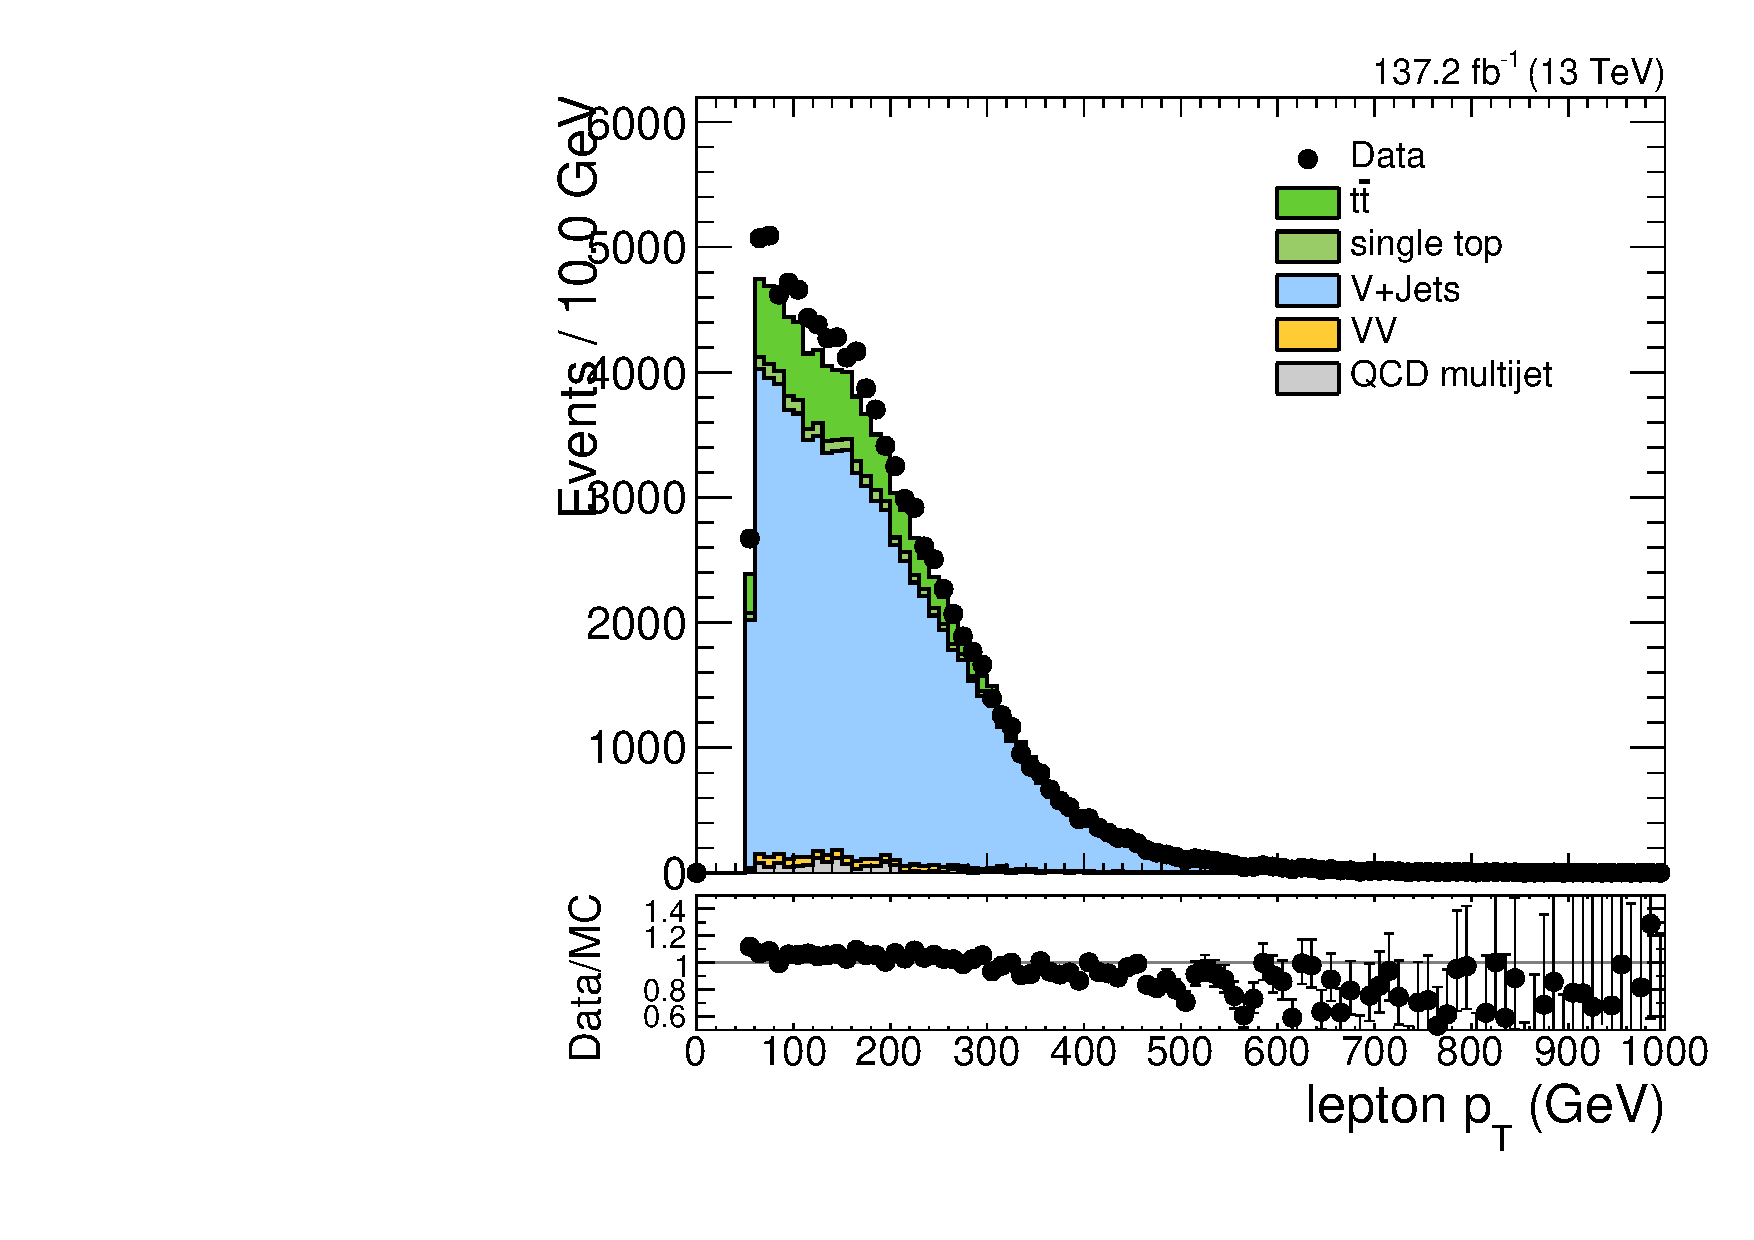
\includegraphics[width=0.4\textwidth]{fig/analysis/SB_b1_mu_allP_allC_allE_Run2_lnujj_l1_l_pt.pdf}
  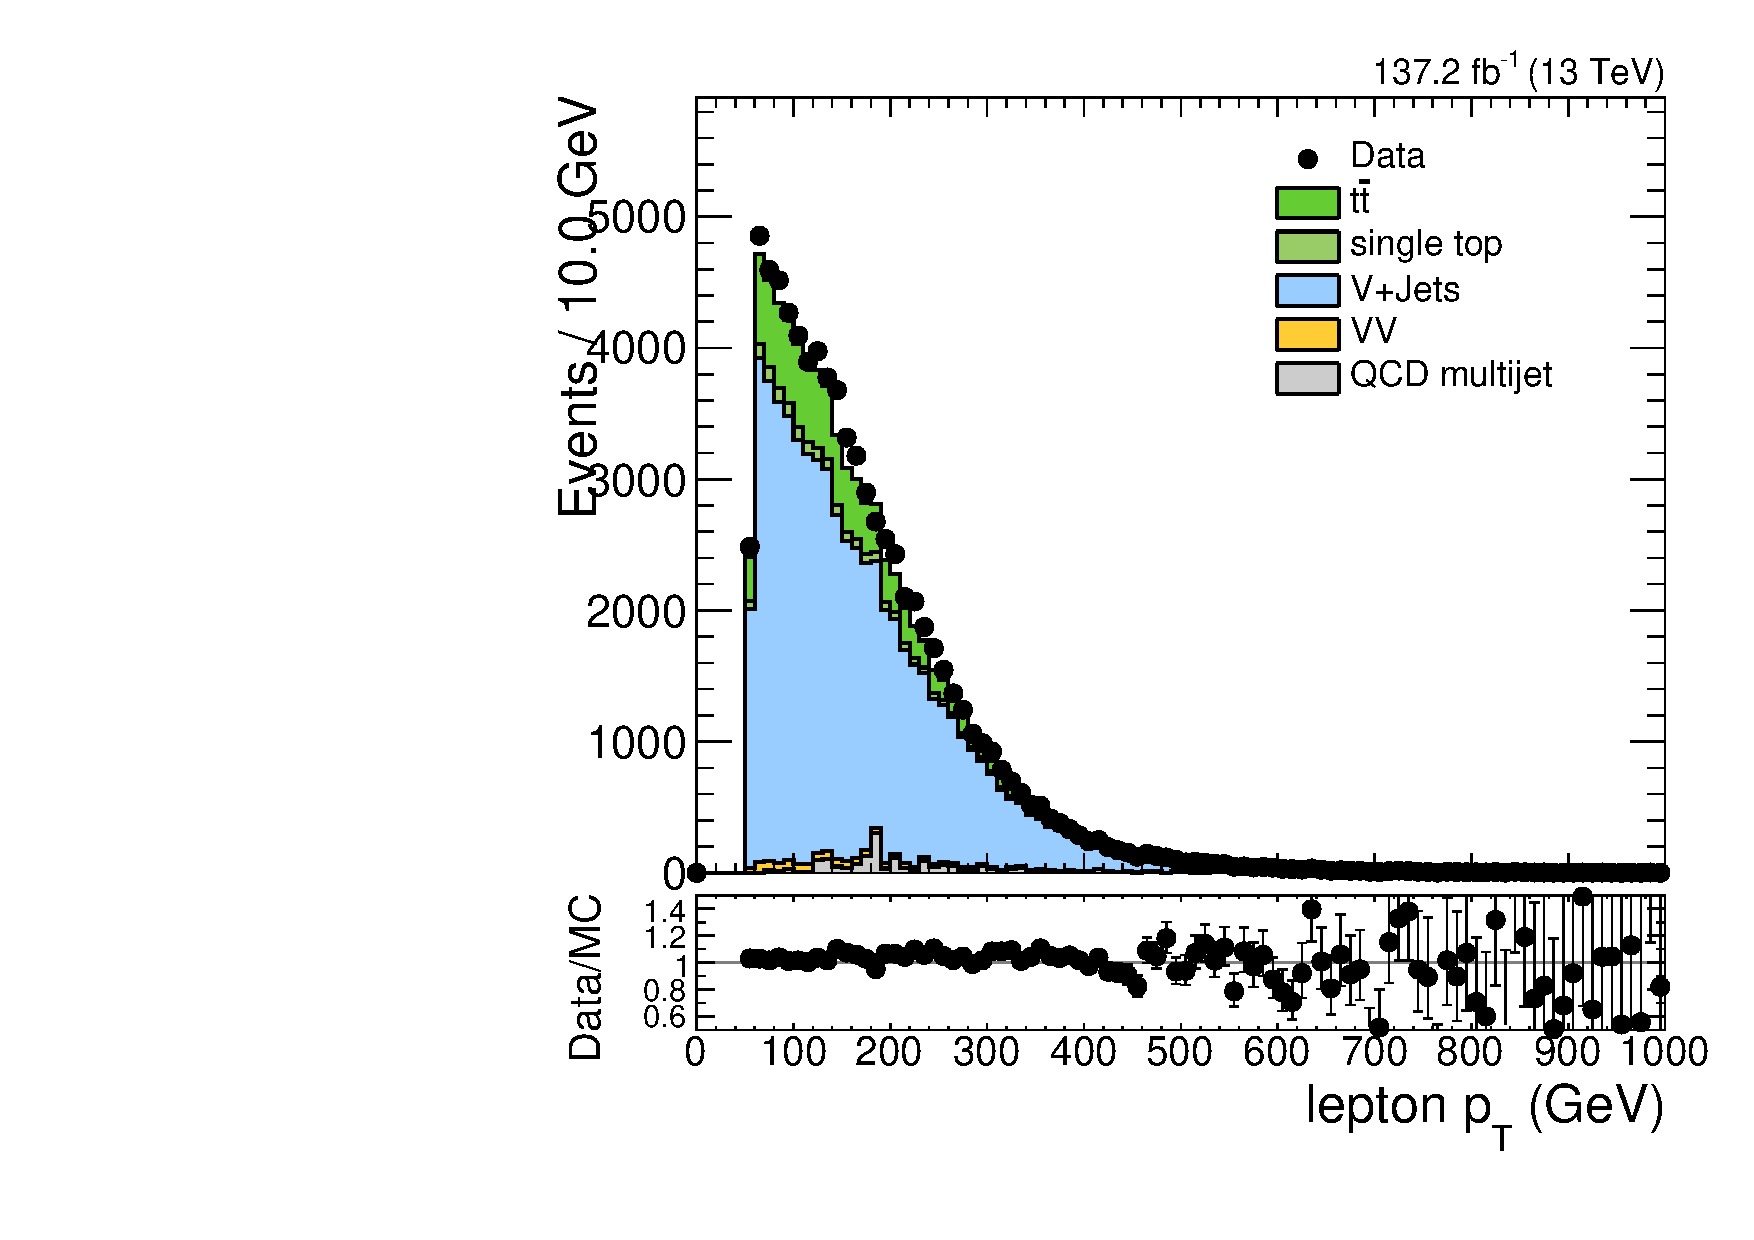
\includegraphics[width=0.4\textwidth]{fig/analysis/SB_b1_e_allP_allC_allE_Run2_lnujj_l1_l_pt.pdf}\\
  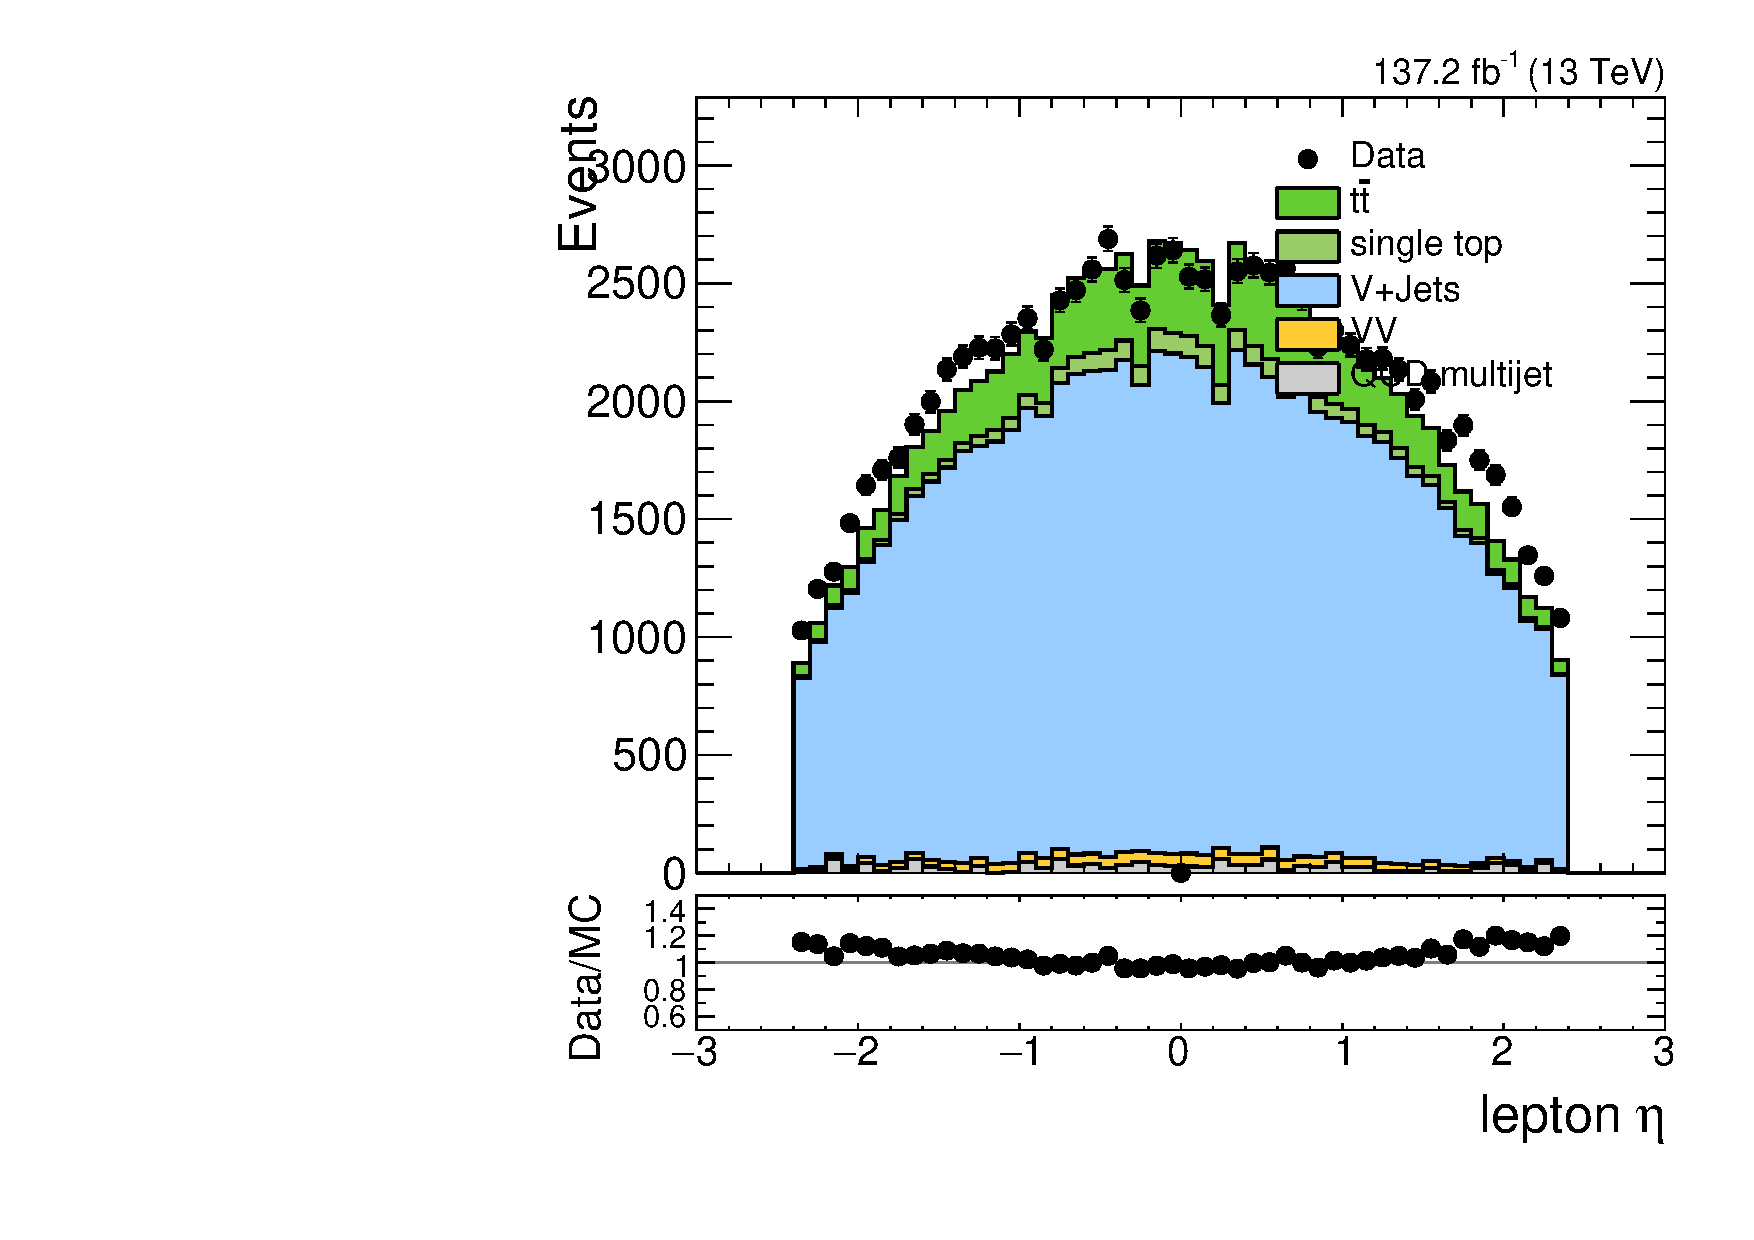
\includegraphics[width=0.4\textwidth]{fig/analysis/SB_b1_mu_allP_allC_allE_Run2_lnujj_l1_l_eta.pdf}
  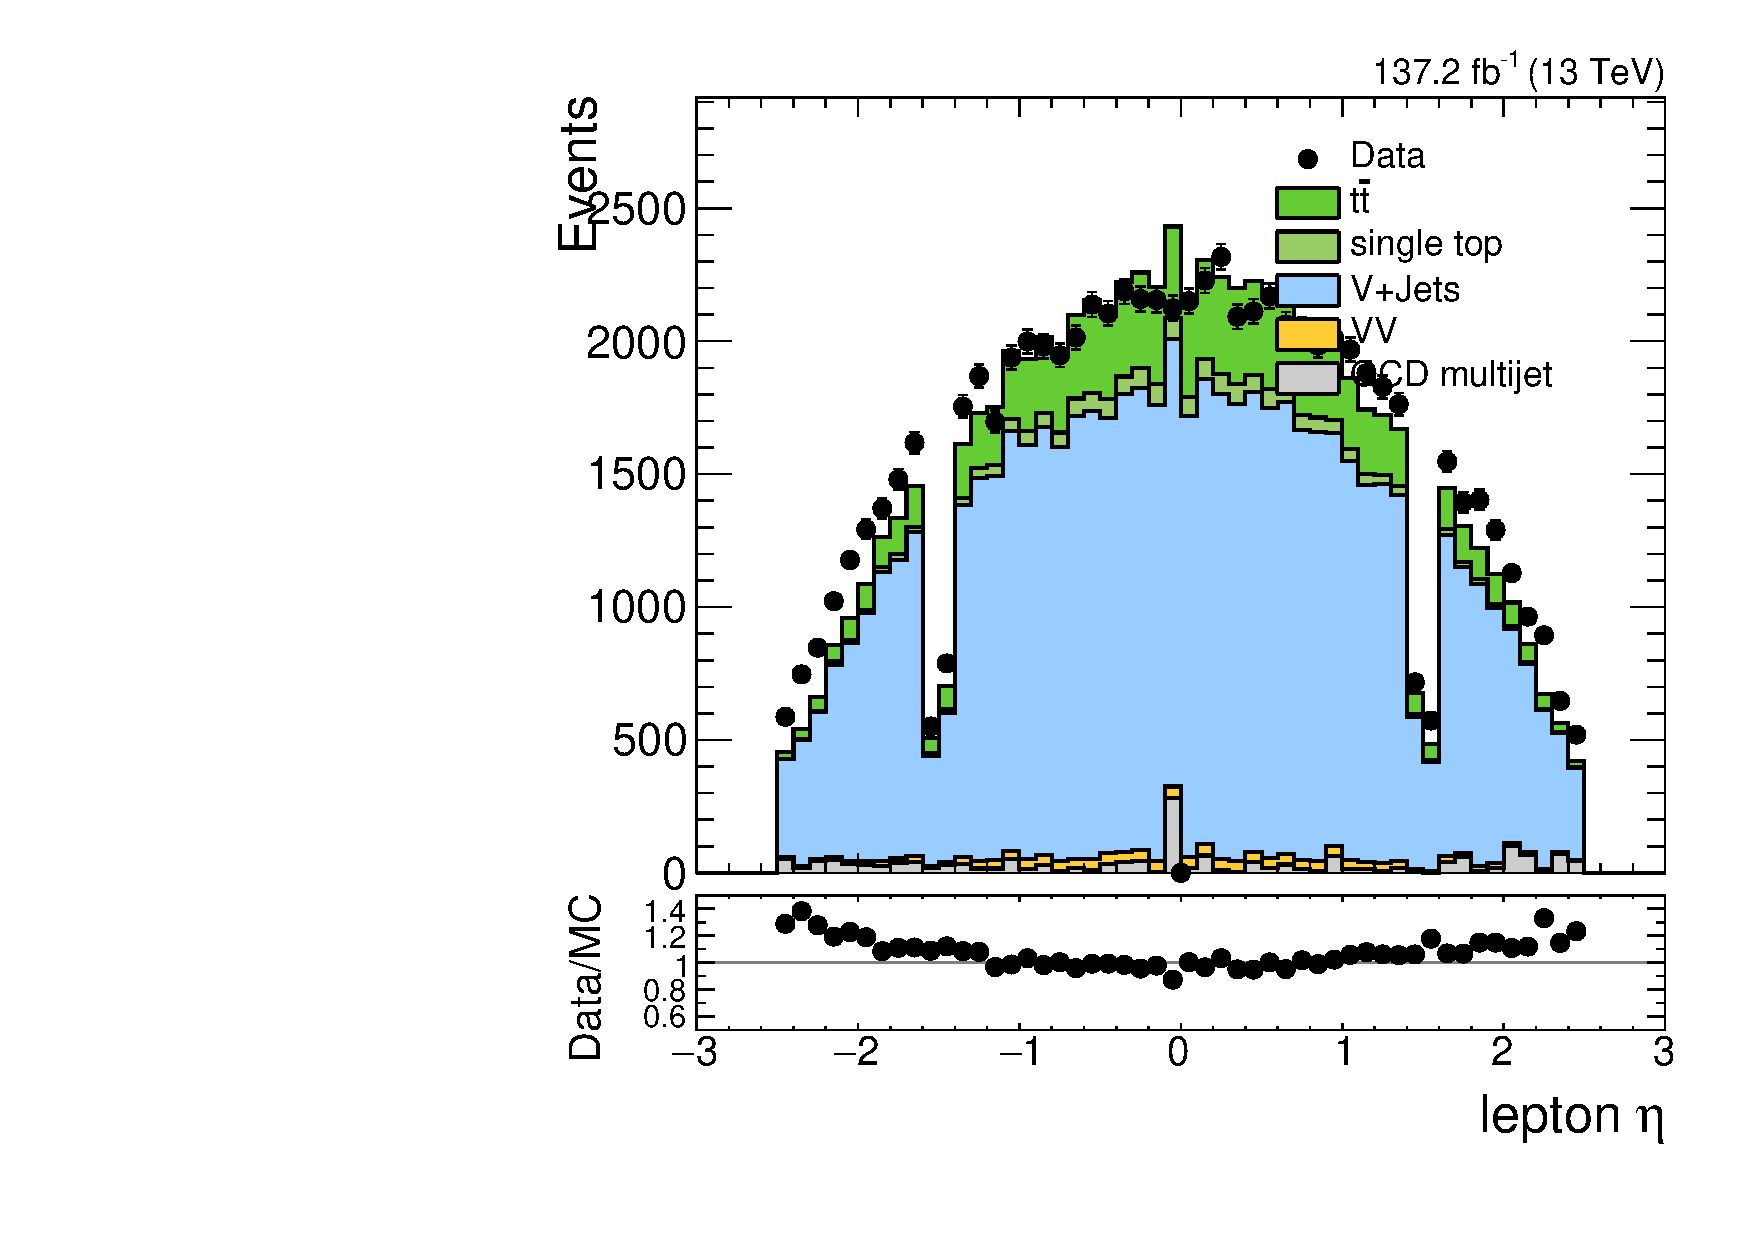
\includegraphics[width=0.4\textwidth]{fig/analysis/SB_b1_e_allP_allC_allE_Run2_lnujj_l1_l_eta.pdf}\\
  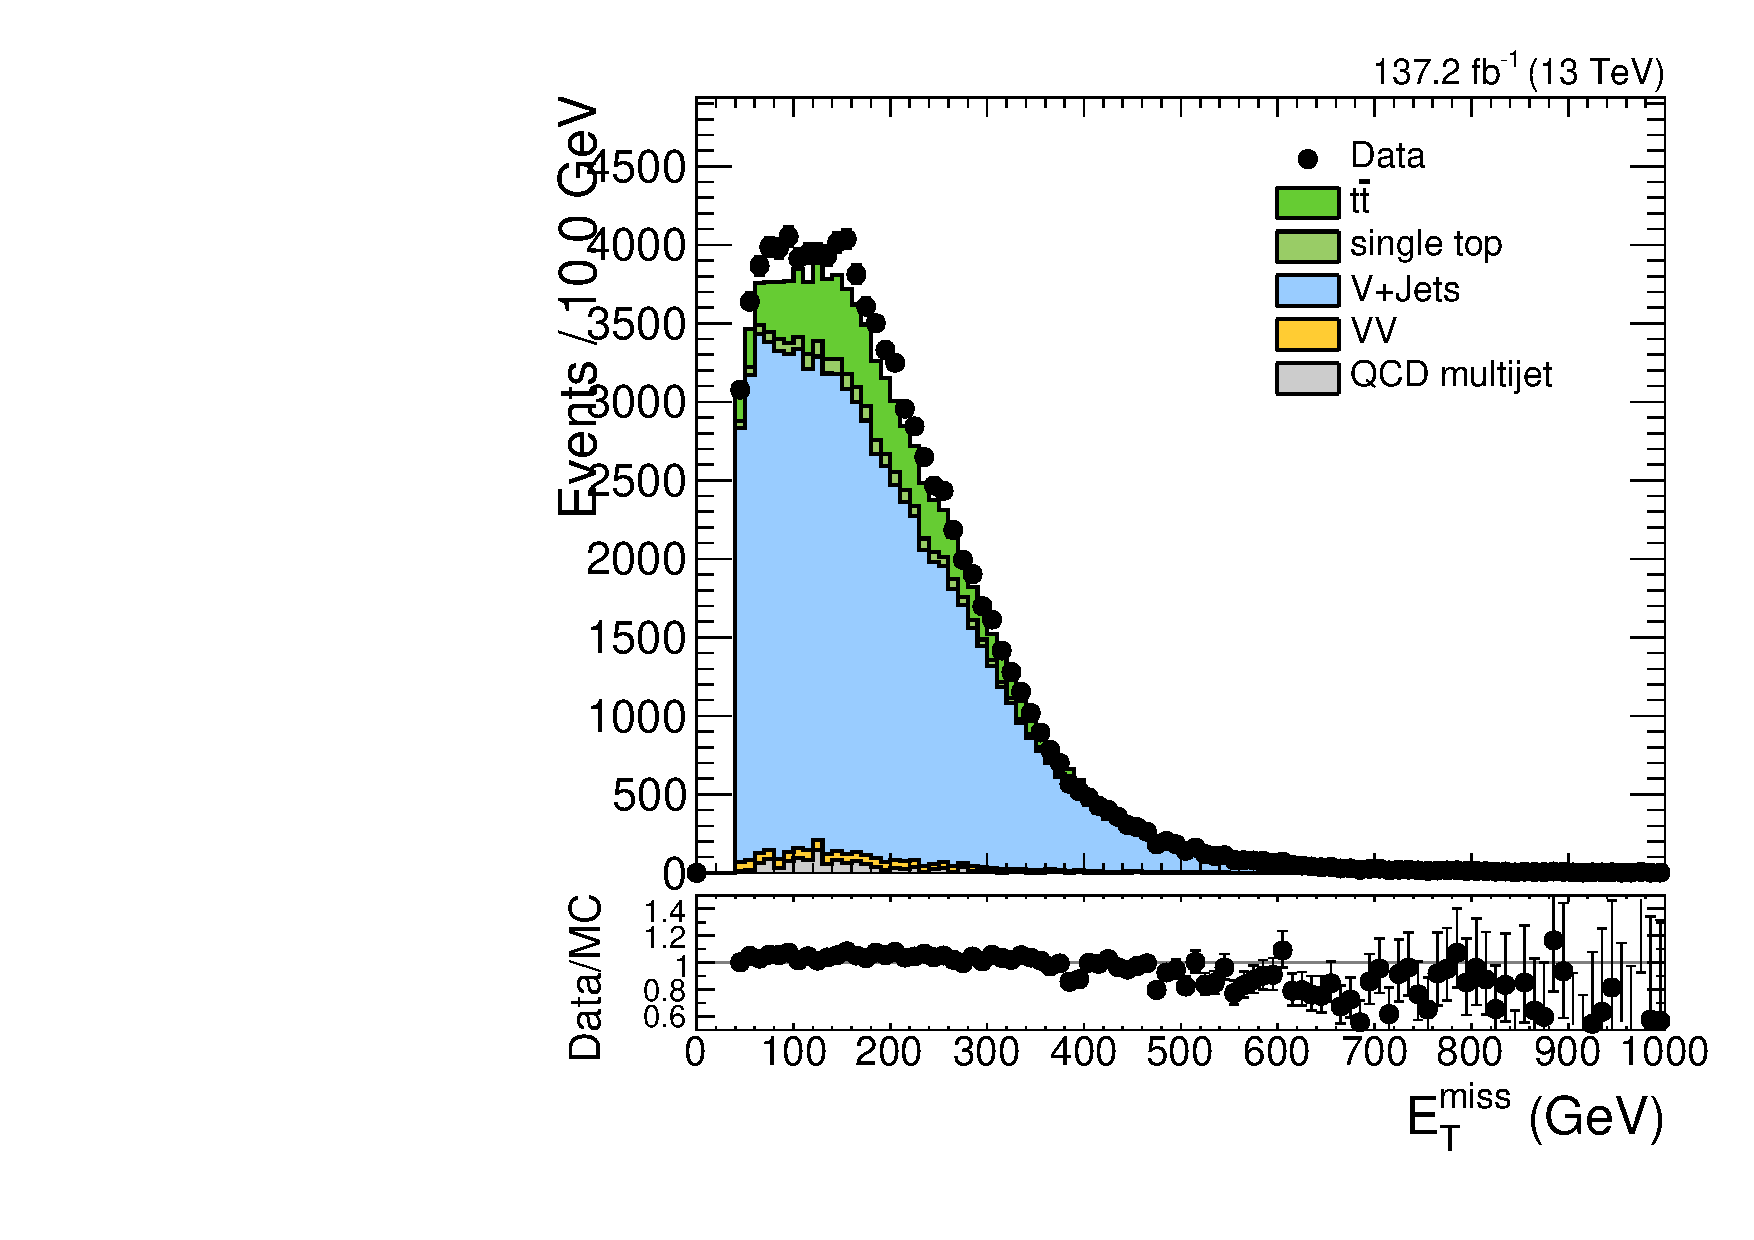
\includegraphics[width=0.4\textwidth]{fig/analysis/SB_b1_mu_allP_allC_allE_Run2_met_pt.pdf}
  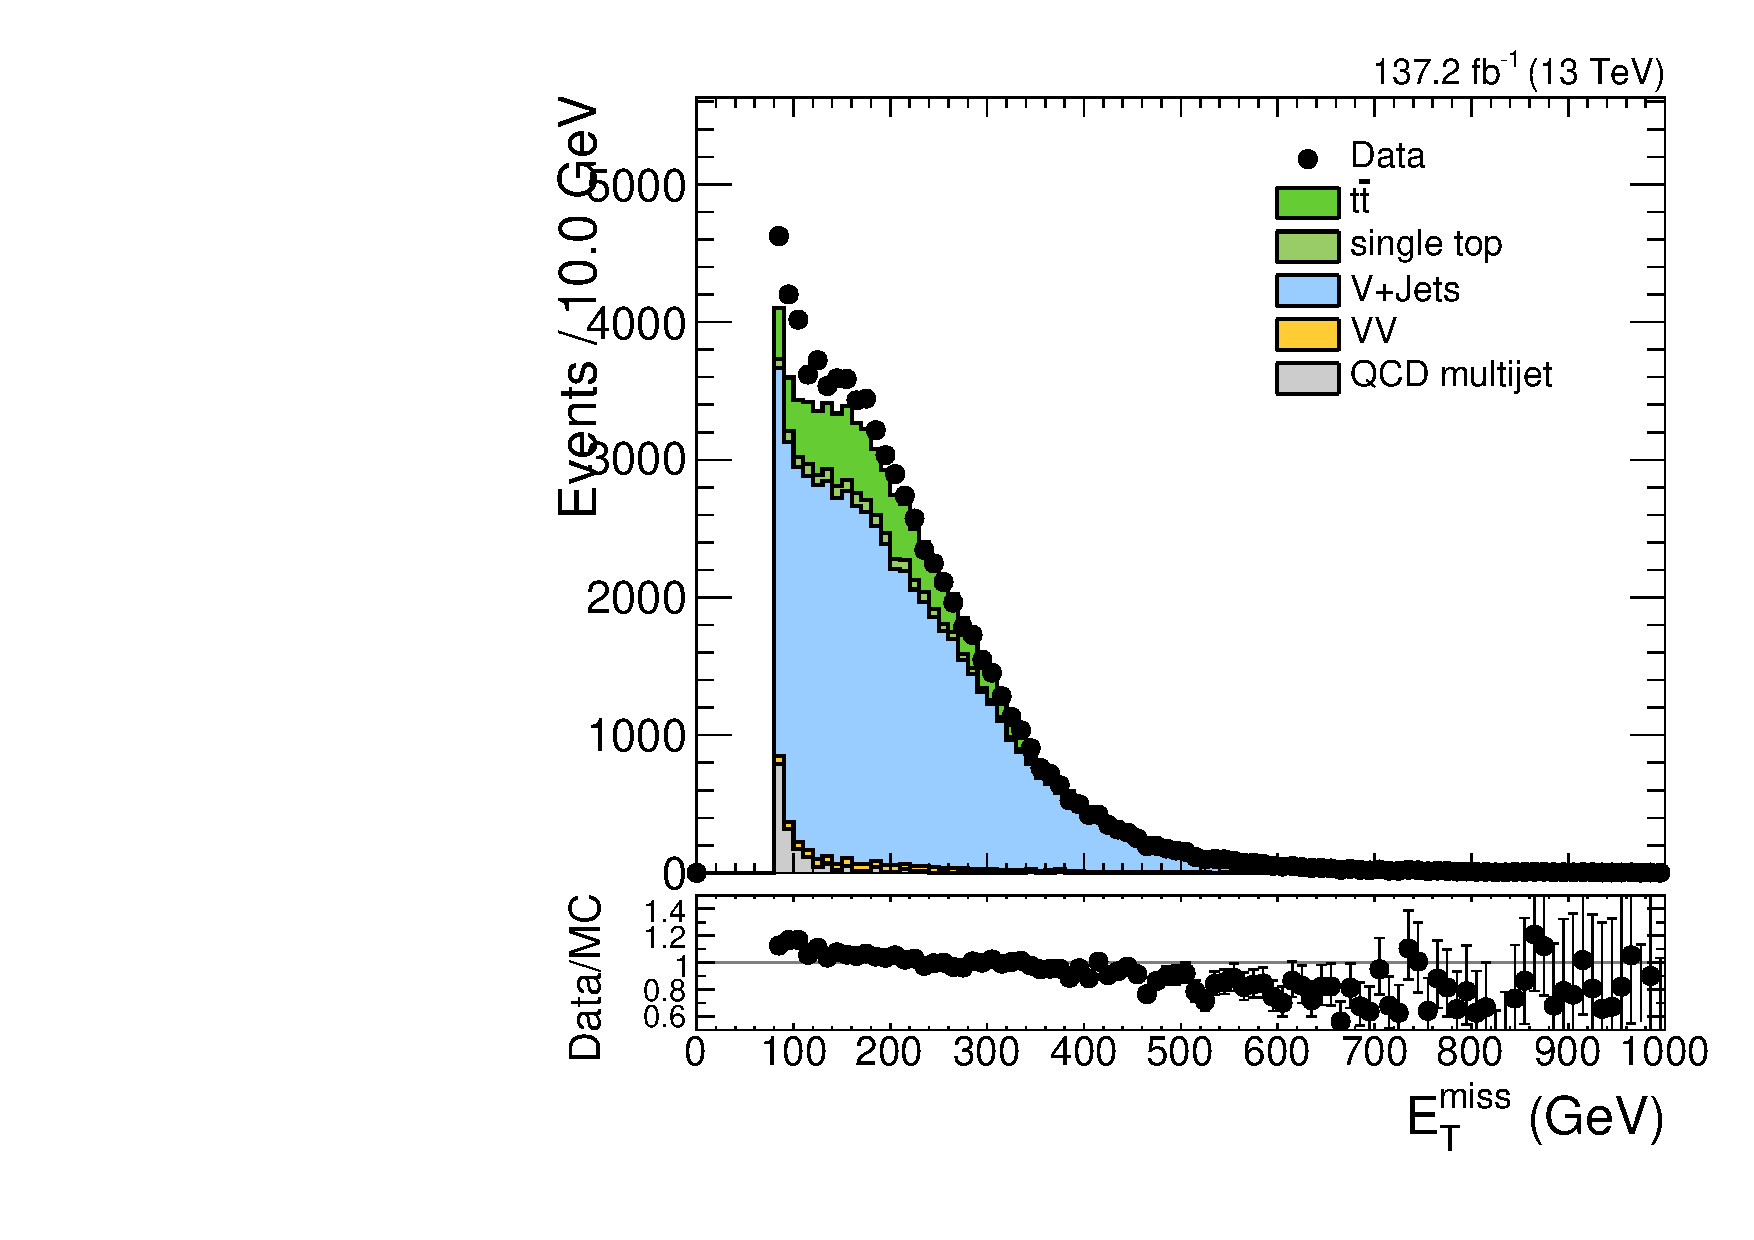
\includegraphics[width=0.4\textwidth]{fig/analysis/SB_b1_e_allP_allC_allE_Run2_met_pt.pdf}\\
  \caption{
    Comparison plots between data and MC from Run 2 for different \Wlep-related observables, in the jet mass sideband.
    From top to bottom: lepton \pt, lepton $\eta$, \Etmiss.
    Left: muon channel, right: electron channel.
  }
  \label{fig:SB_controlPlotsRun2_1}
\end{figure}

\begin{figure}[htbp]
  \centering
  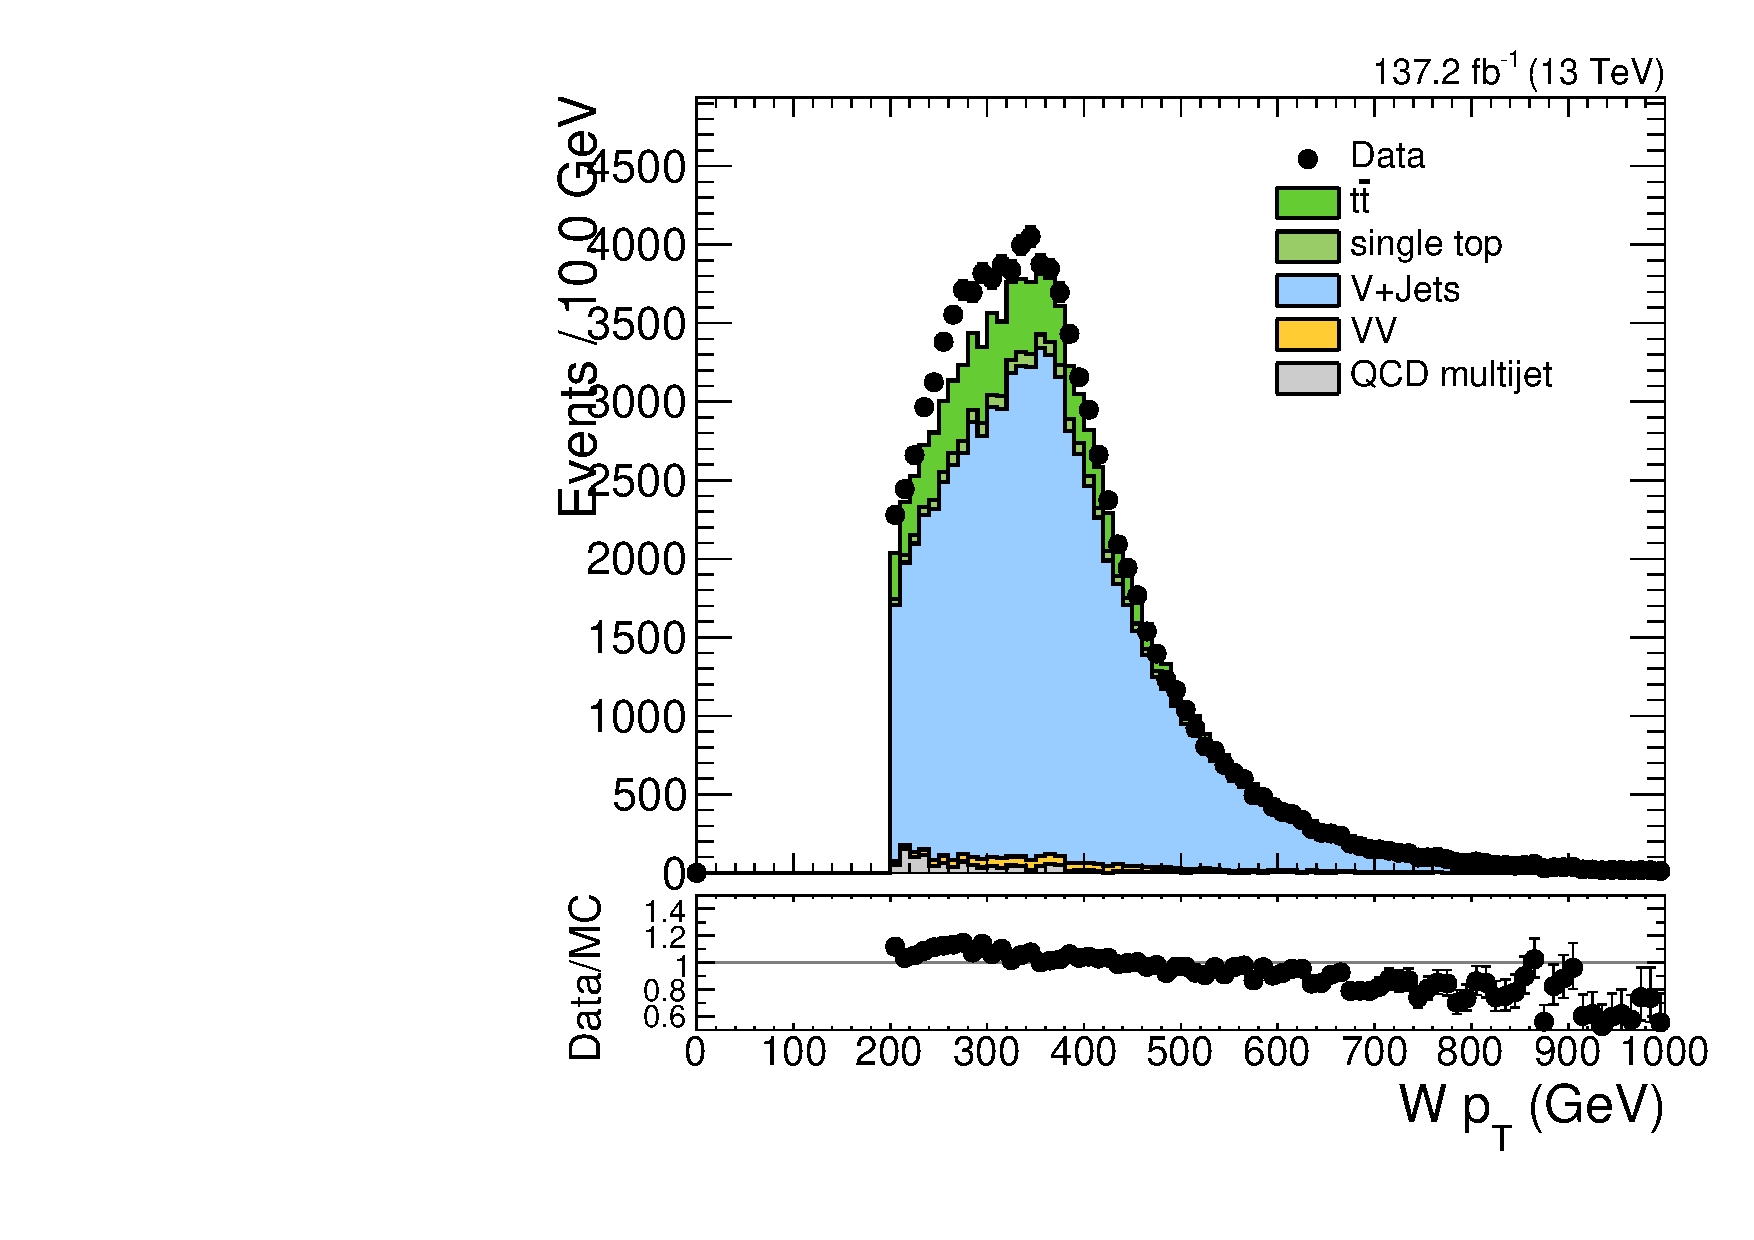
\includegraphics[width=0.4\textwidth]{fig/analysis/SB_b1_mu_allP_allC_allE_Run2_lnujj_l1_pt.pdf}
  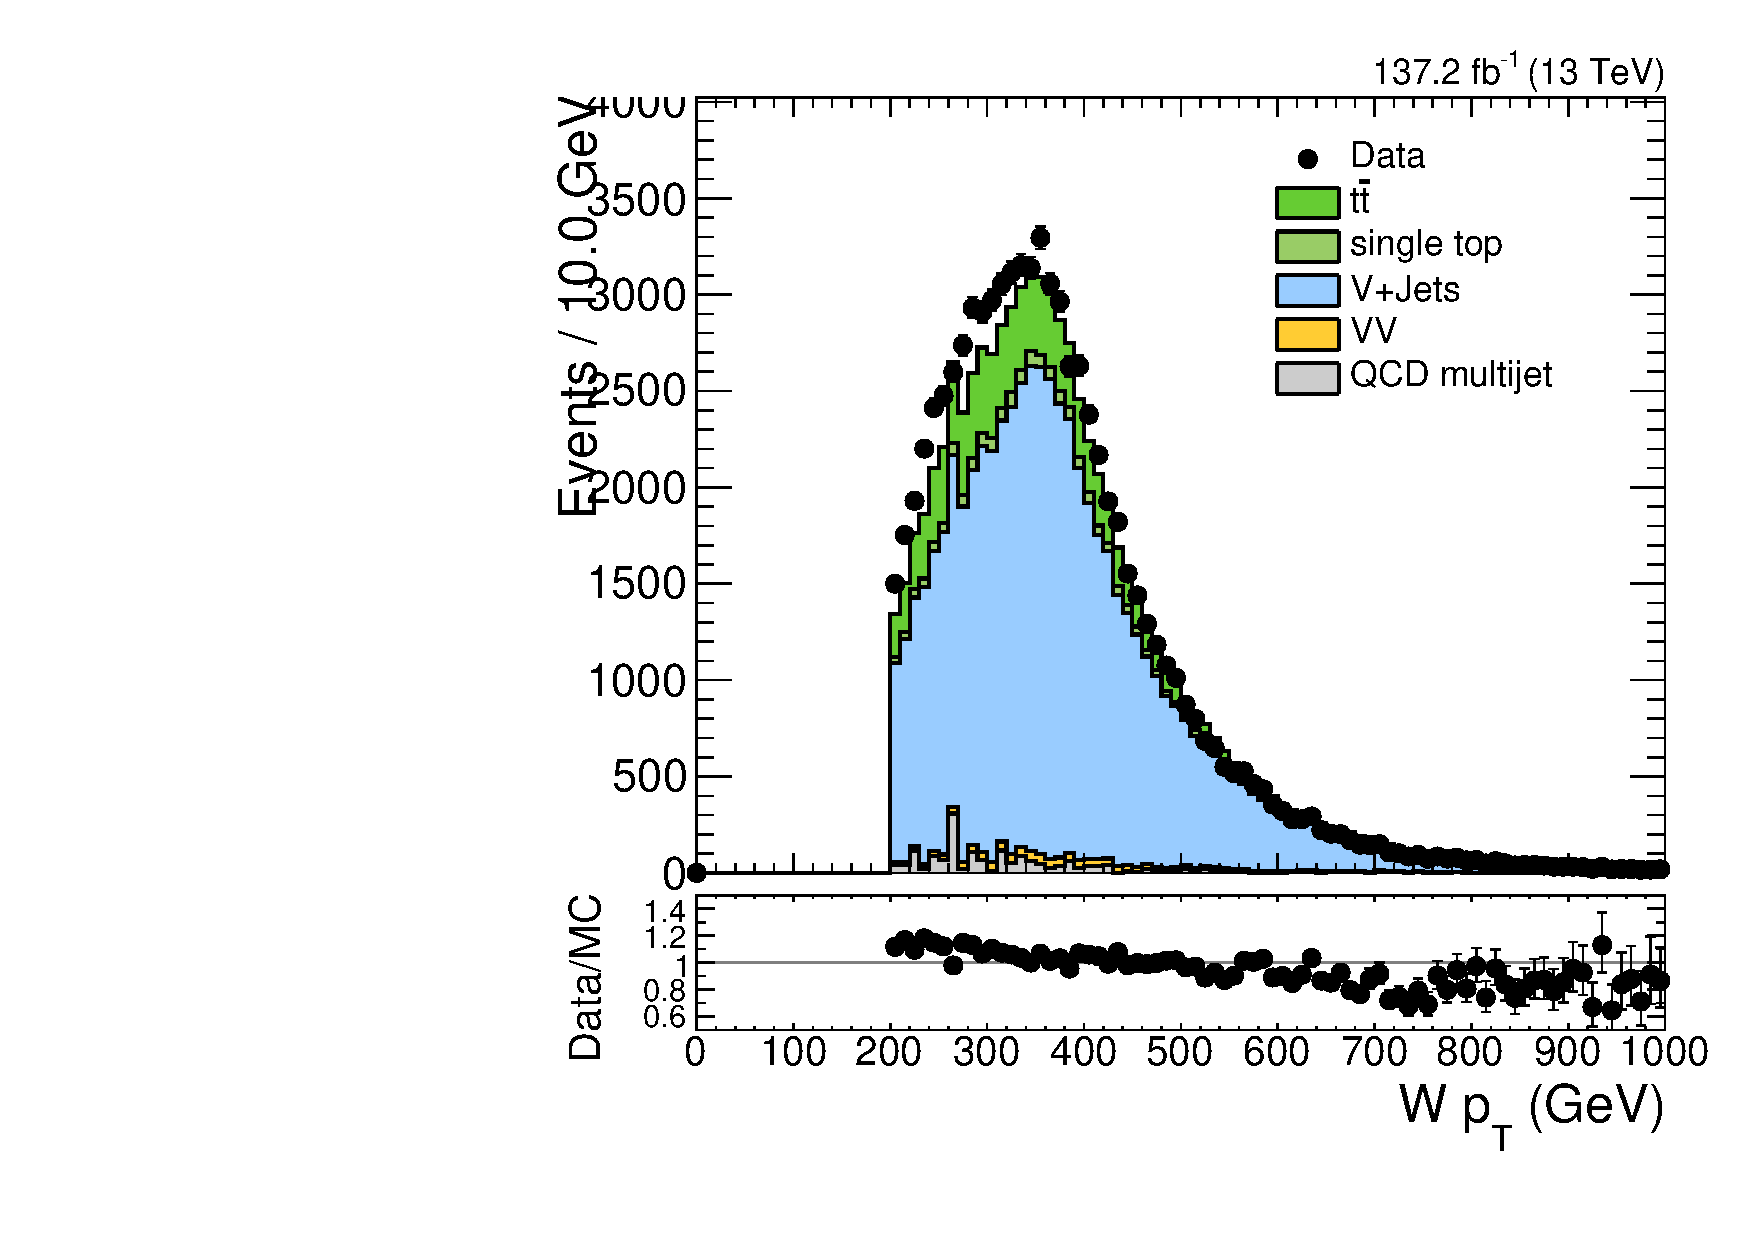
\includegraphics[width=0.4\textwidth]{fig/analysis/SB_b1_e_allP_allC_allE_Run2_lnujj_l1_pt.pdf}\\
  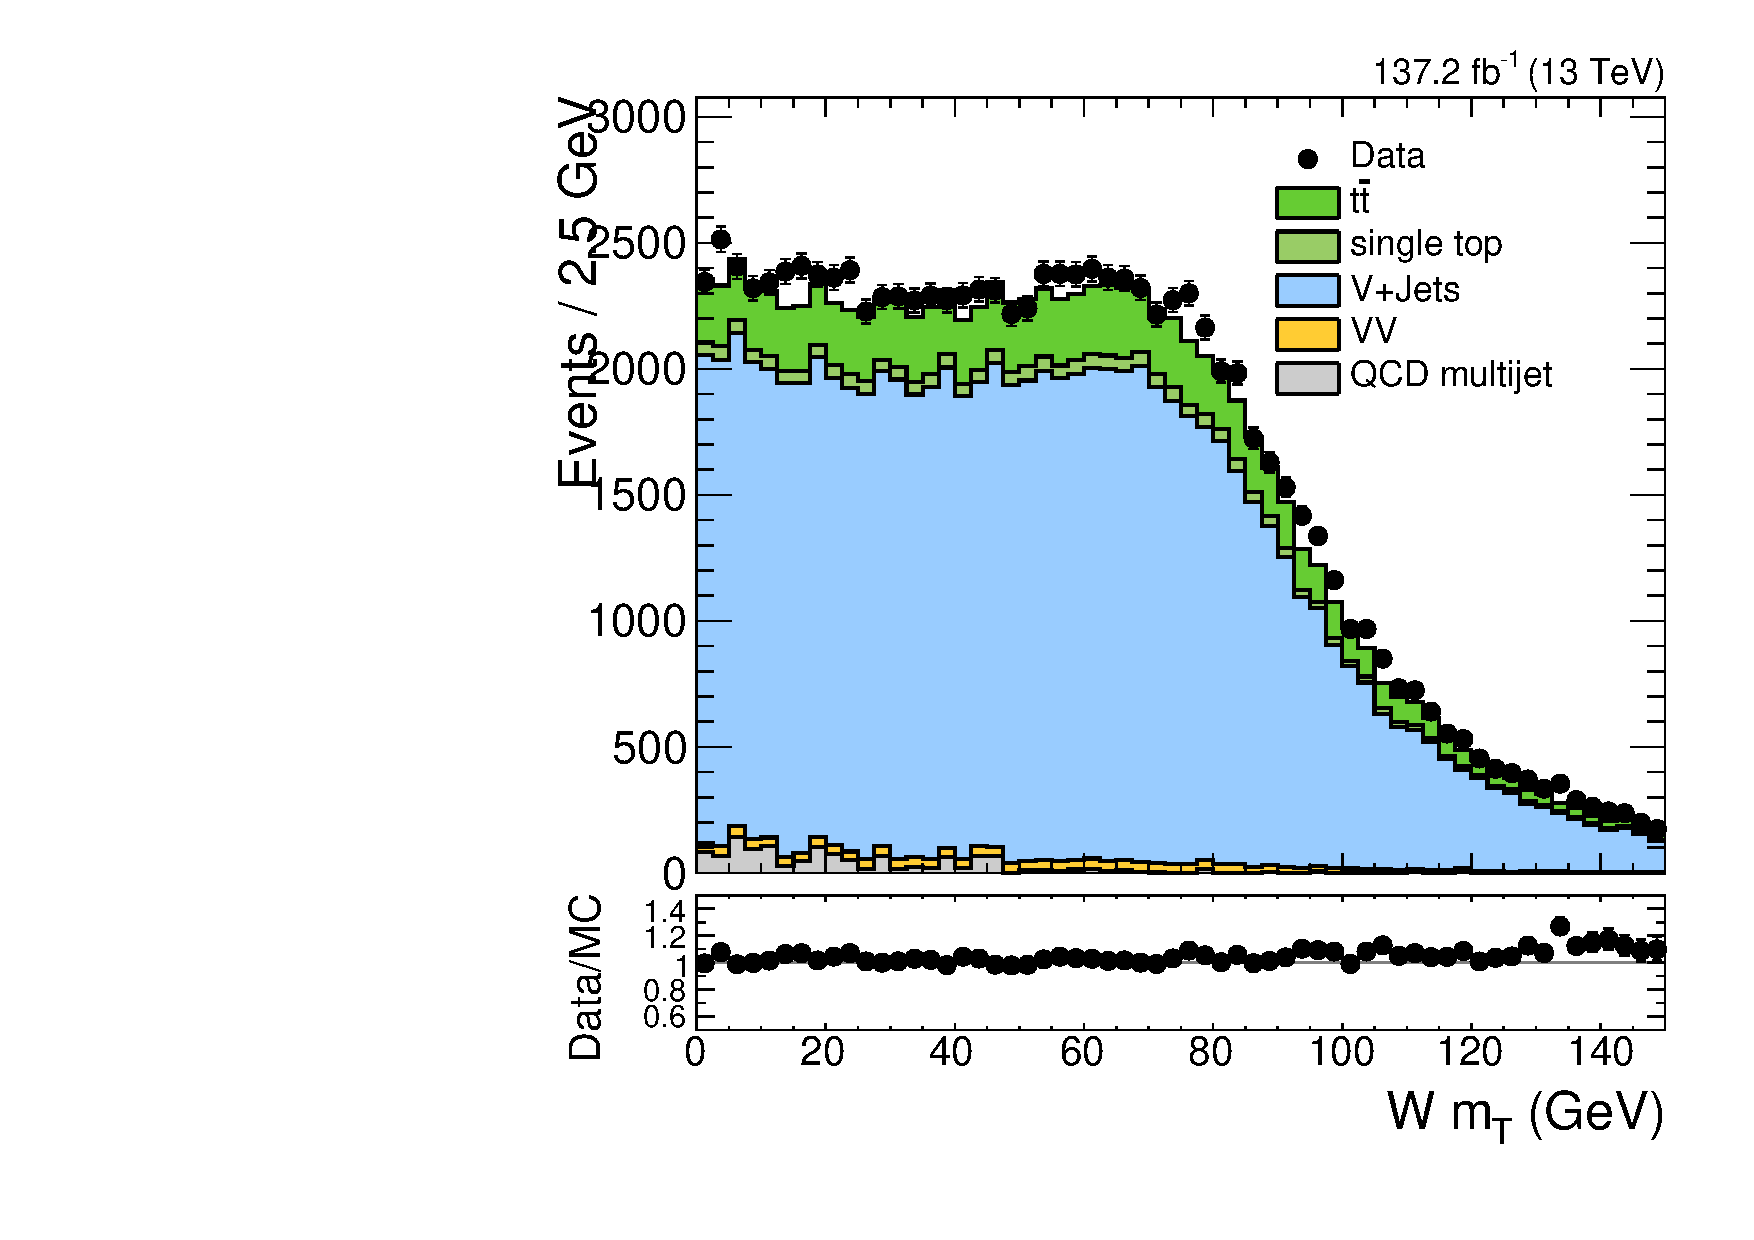
\includegraphics[width=0.4\textwidth]{fig/analysis/SB_b1_mu_allP_allC_allE_Run2_lnujj_l1_mt.pdf}
  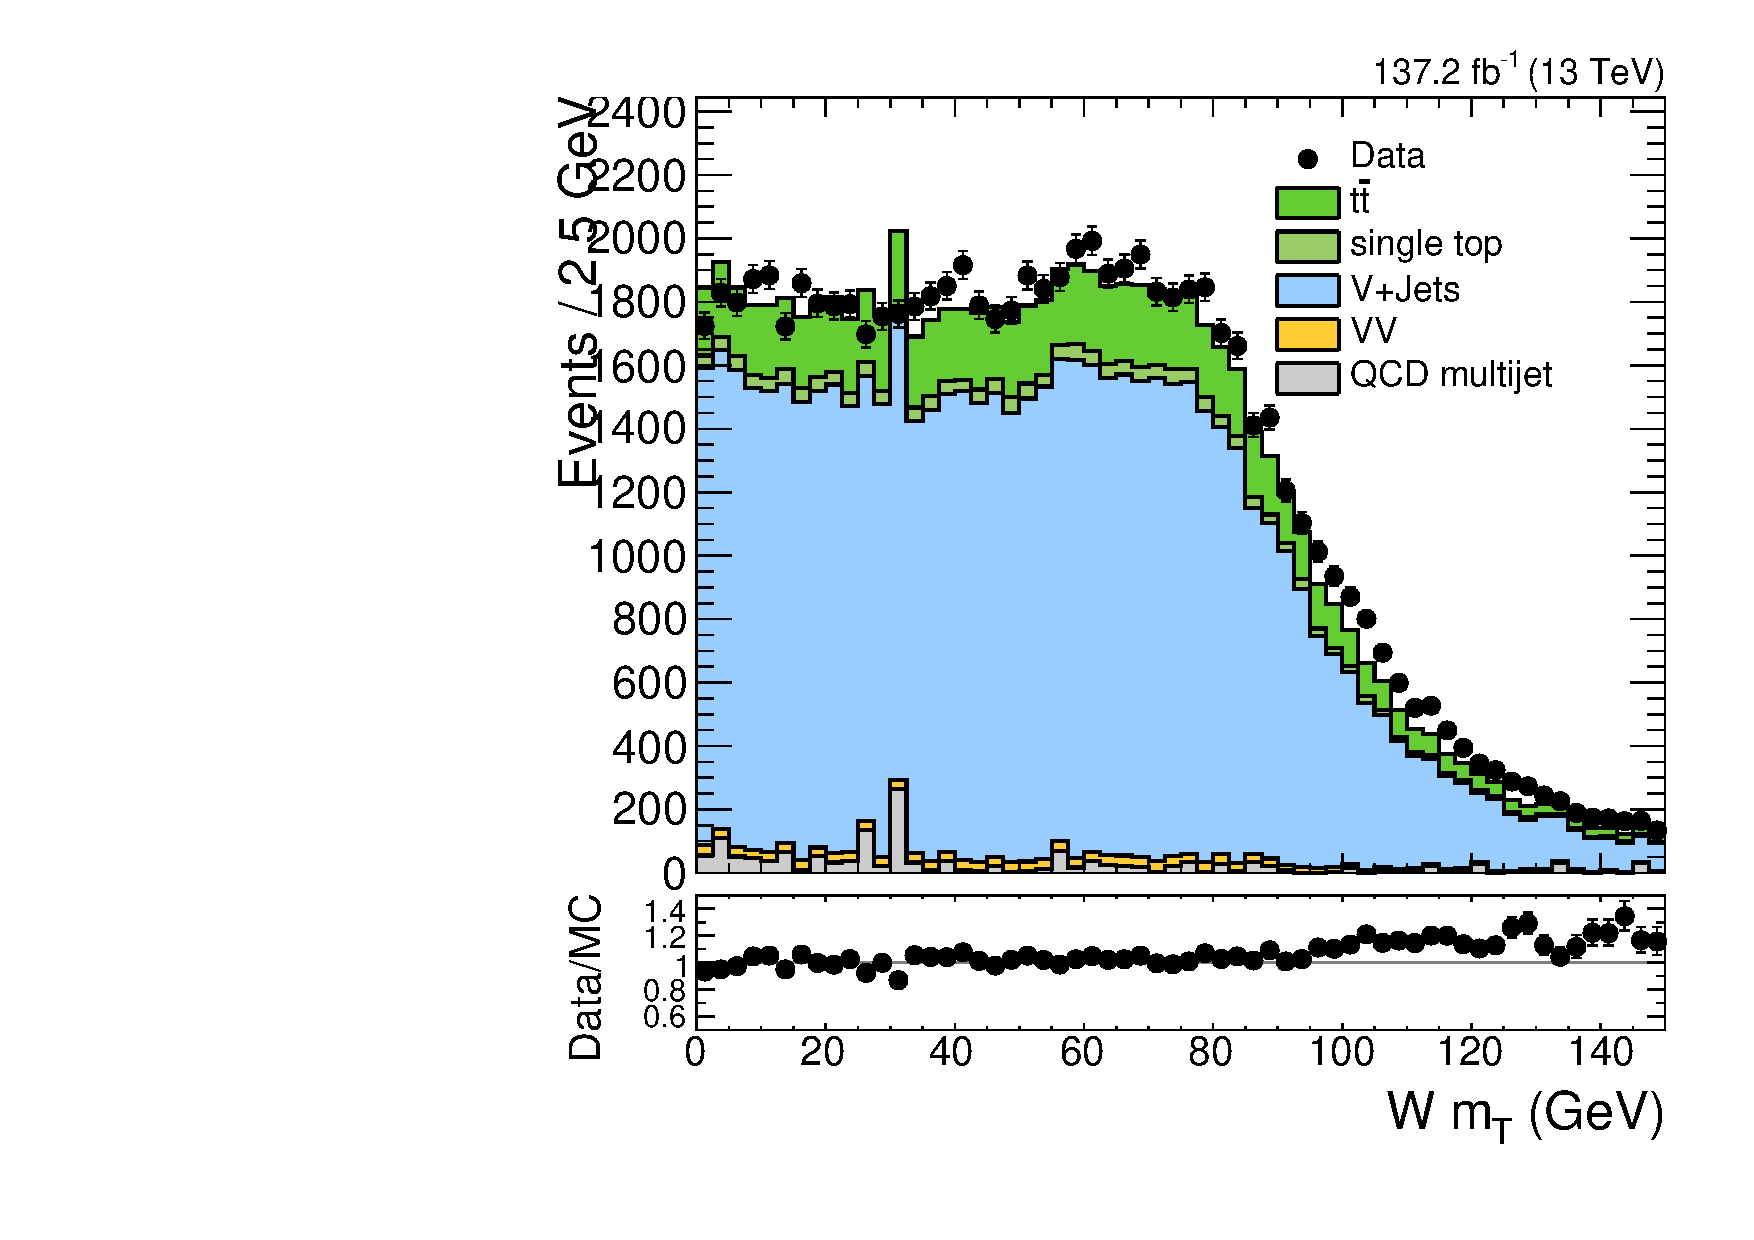
\includegraphics[width=0.4\textwidth]{fig/analysis/SB_b1_e_allP_allC_allE_Run2_lnujj_l1_mt.pdf}\\
  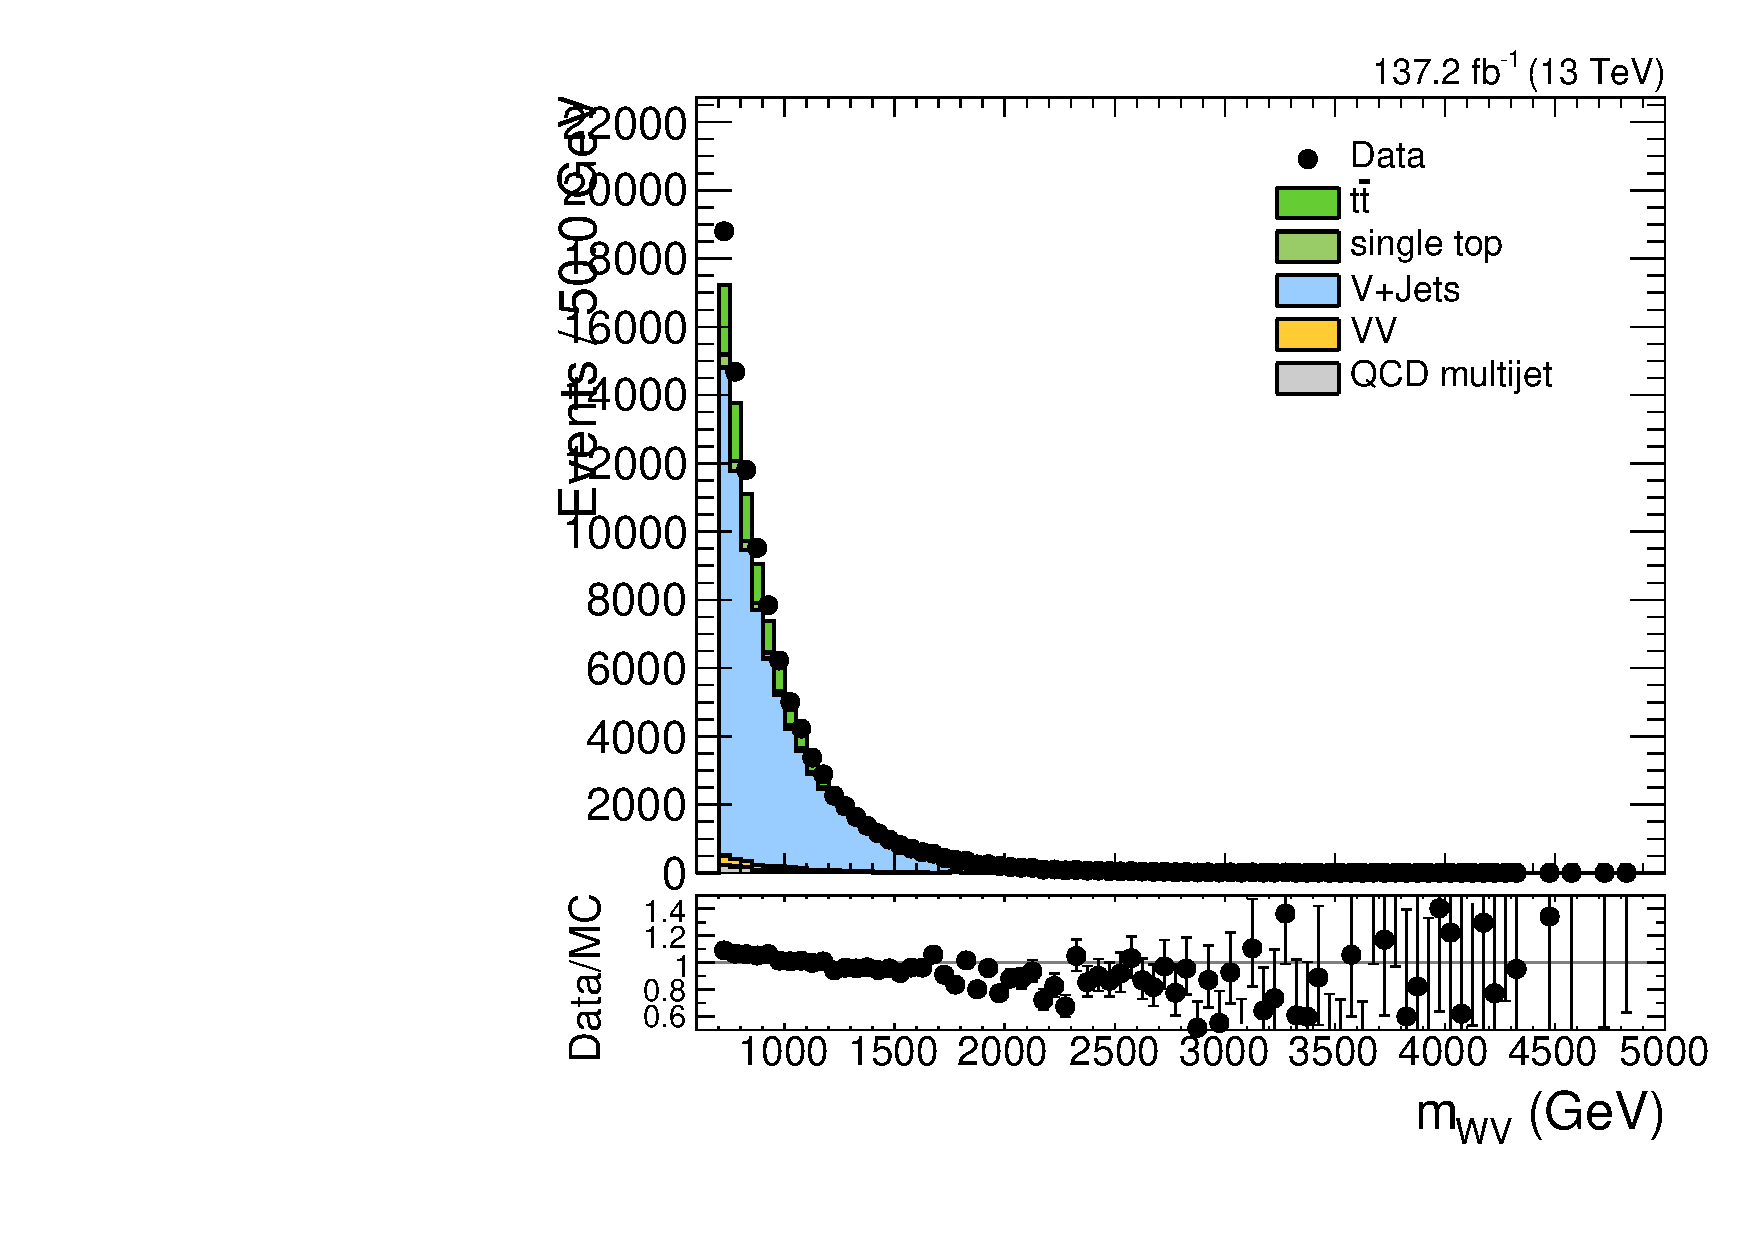
\includegraphics[width=0.4\textwidth]{fig/analysis/SB_b1_mu_allP_allC_allE_Run2_mWV.pdf}
  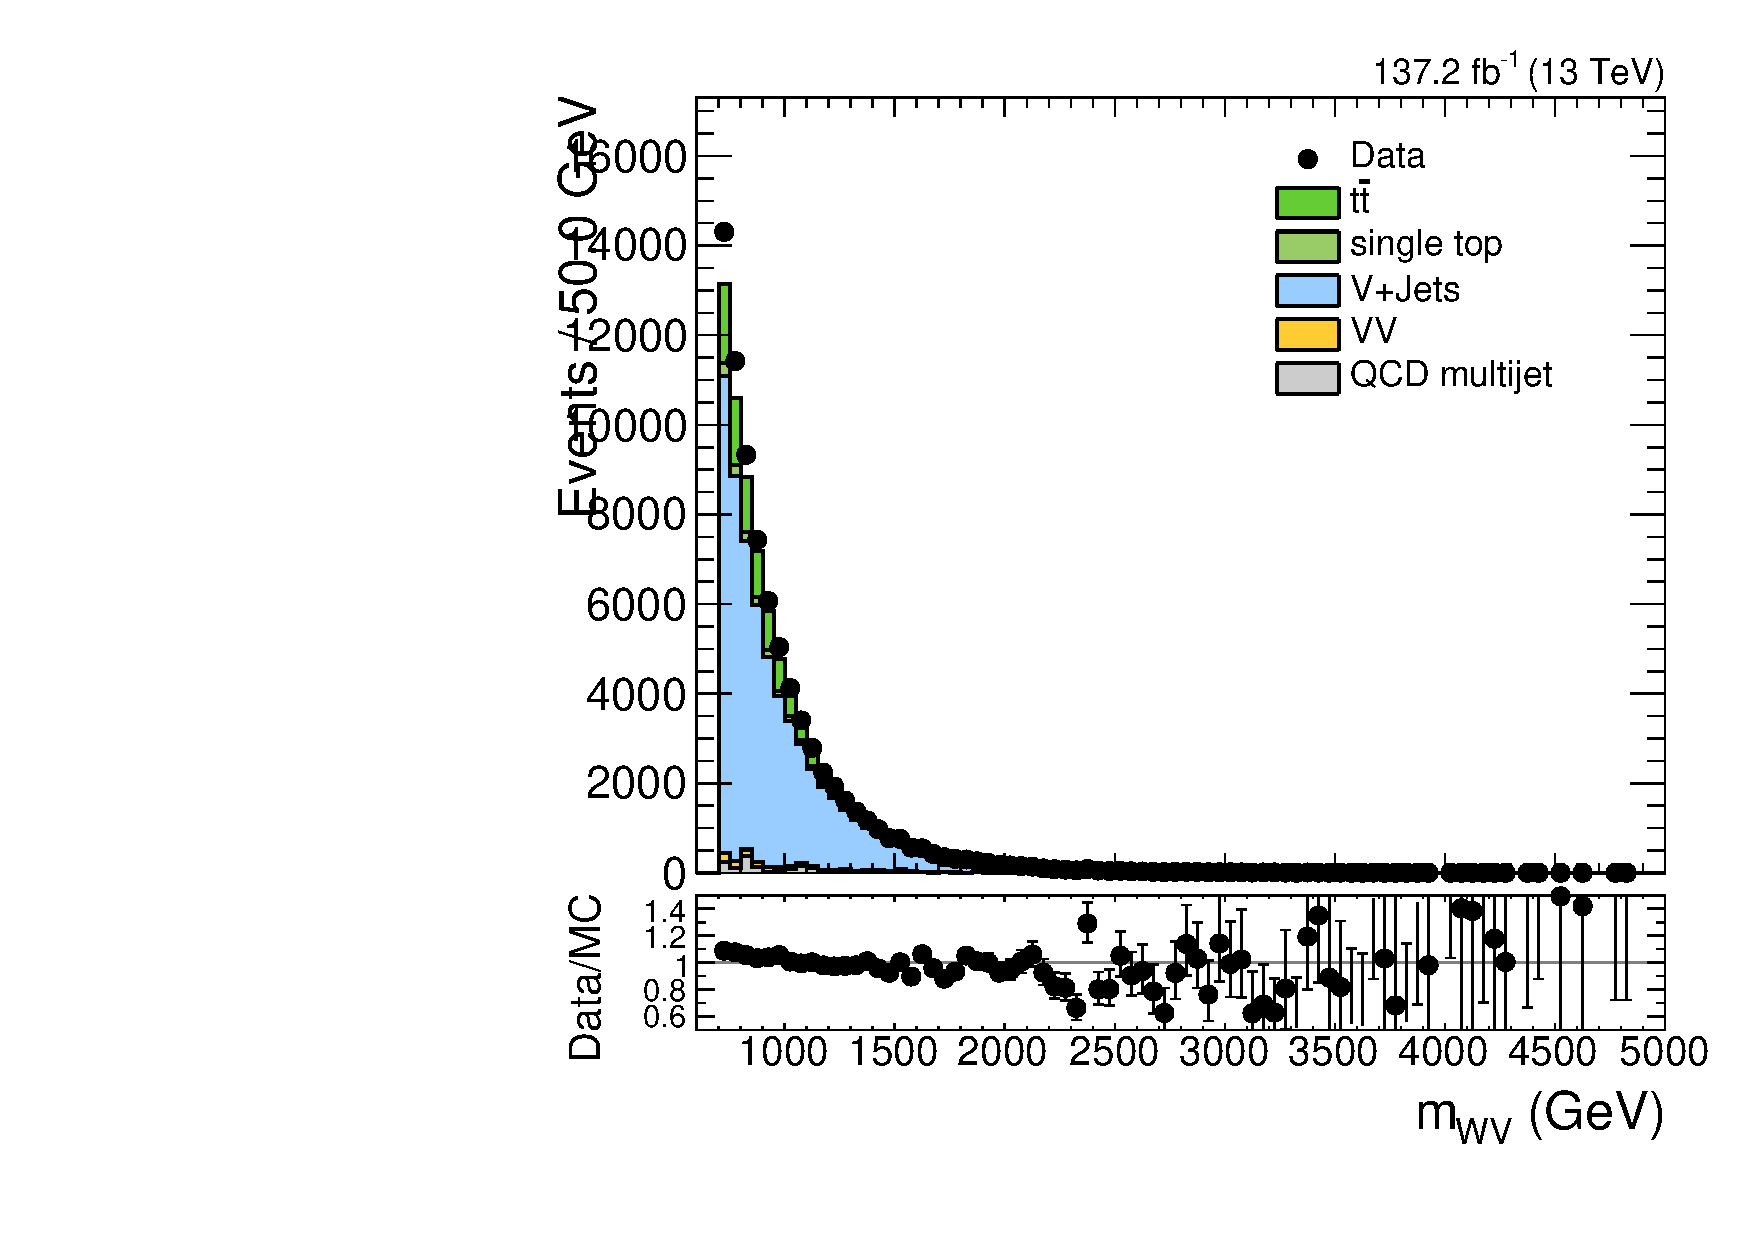
\includegraphics[width=0.4\textwidth]{fig/analysis/SB_b1_e_allP_allC_allE_Run2_mWV.pdf}\\
  \caption{
    Comparison plots between data and MC from Run 2 for different \Wlep-related observables, in the jet mass sideband.
    From top to bottom: \pt of the leptonic W, transverse mass of the leptonic W, diboson invariant mass.
    Left: muon channel, right: electron channel.
  }
  \label{fig:SB_controlPlotsRun2_2}
\end{figure}

\begin{figure}[htbp]
  \centering
  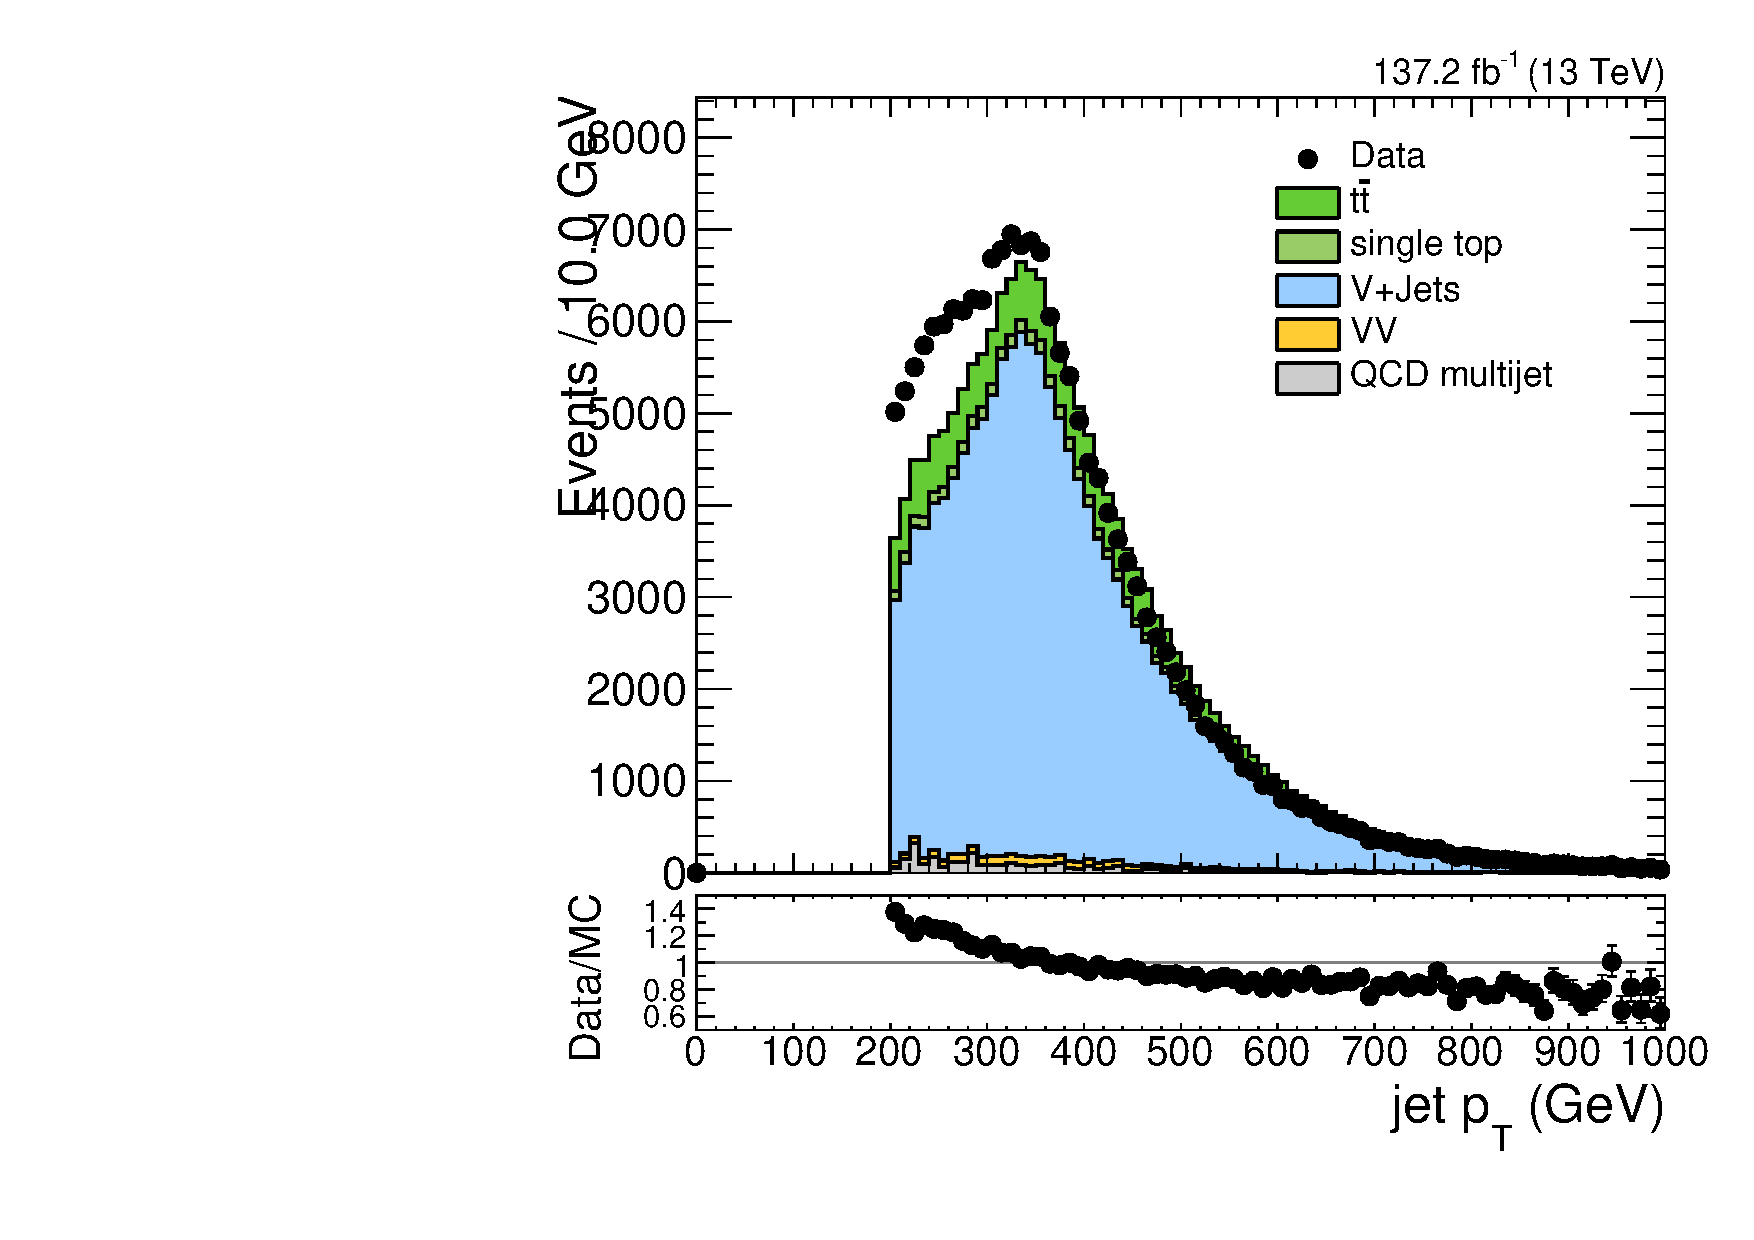
\includegraphics[width=0.4\textwidth]{fig/analysis/SB_b1_allL_allP_allC_allE_Run2_lnujj_l2_pt.pdf}
  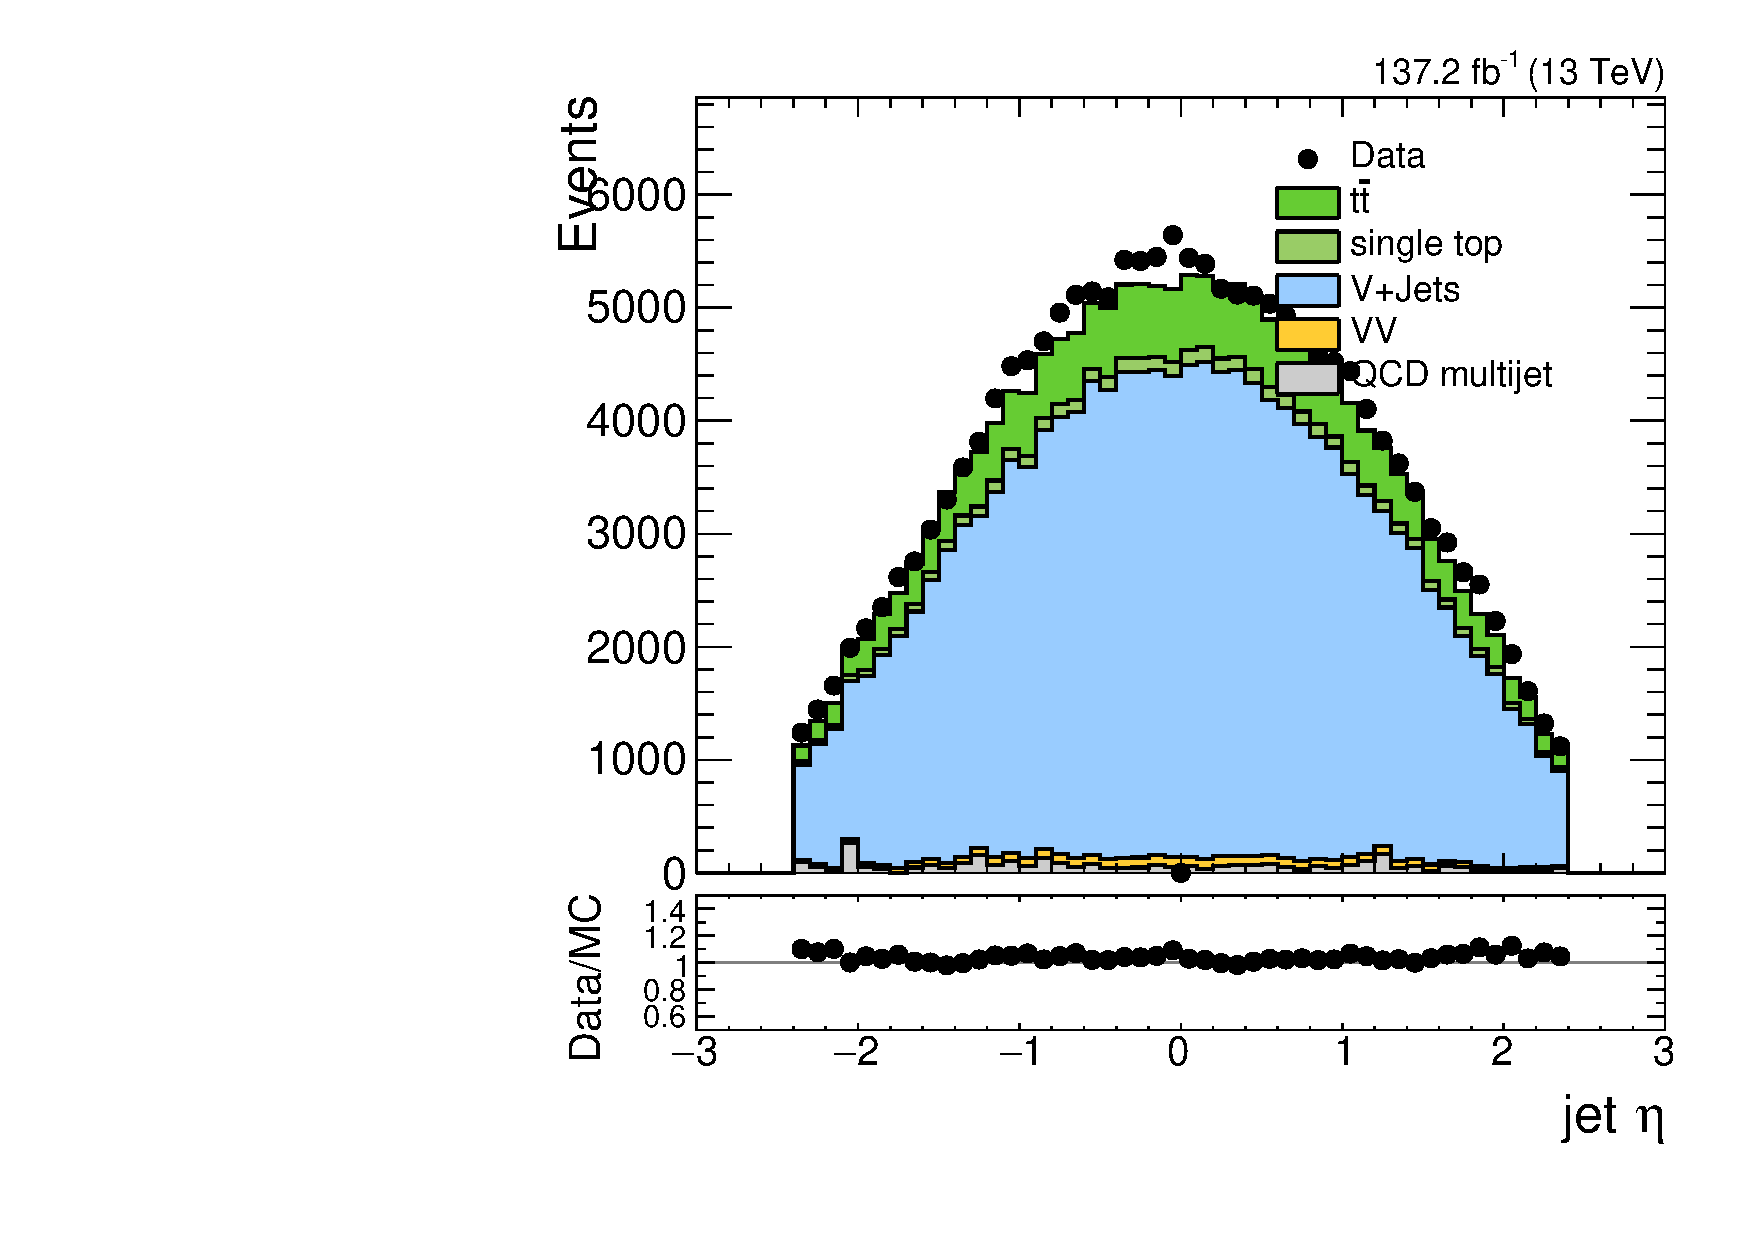
\includegraphics[width=0.4\textwidth]{fig/analysis/SB_b1_allL_allP_allC_allE_Run2_lnujj_l2_eta.pdf}\\
  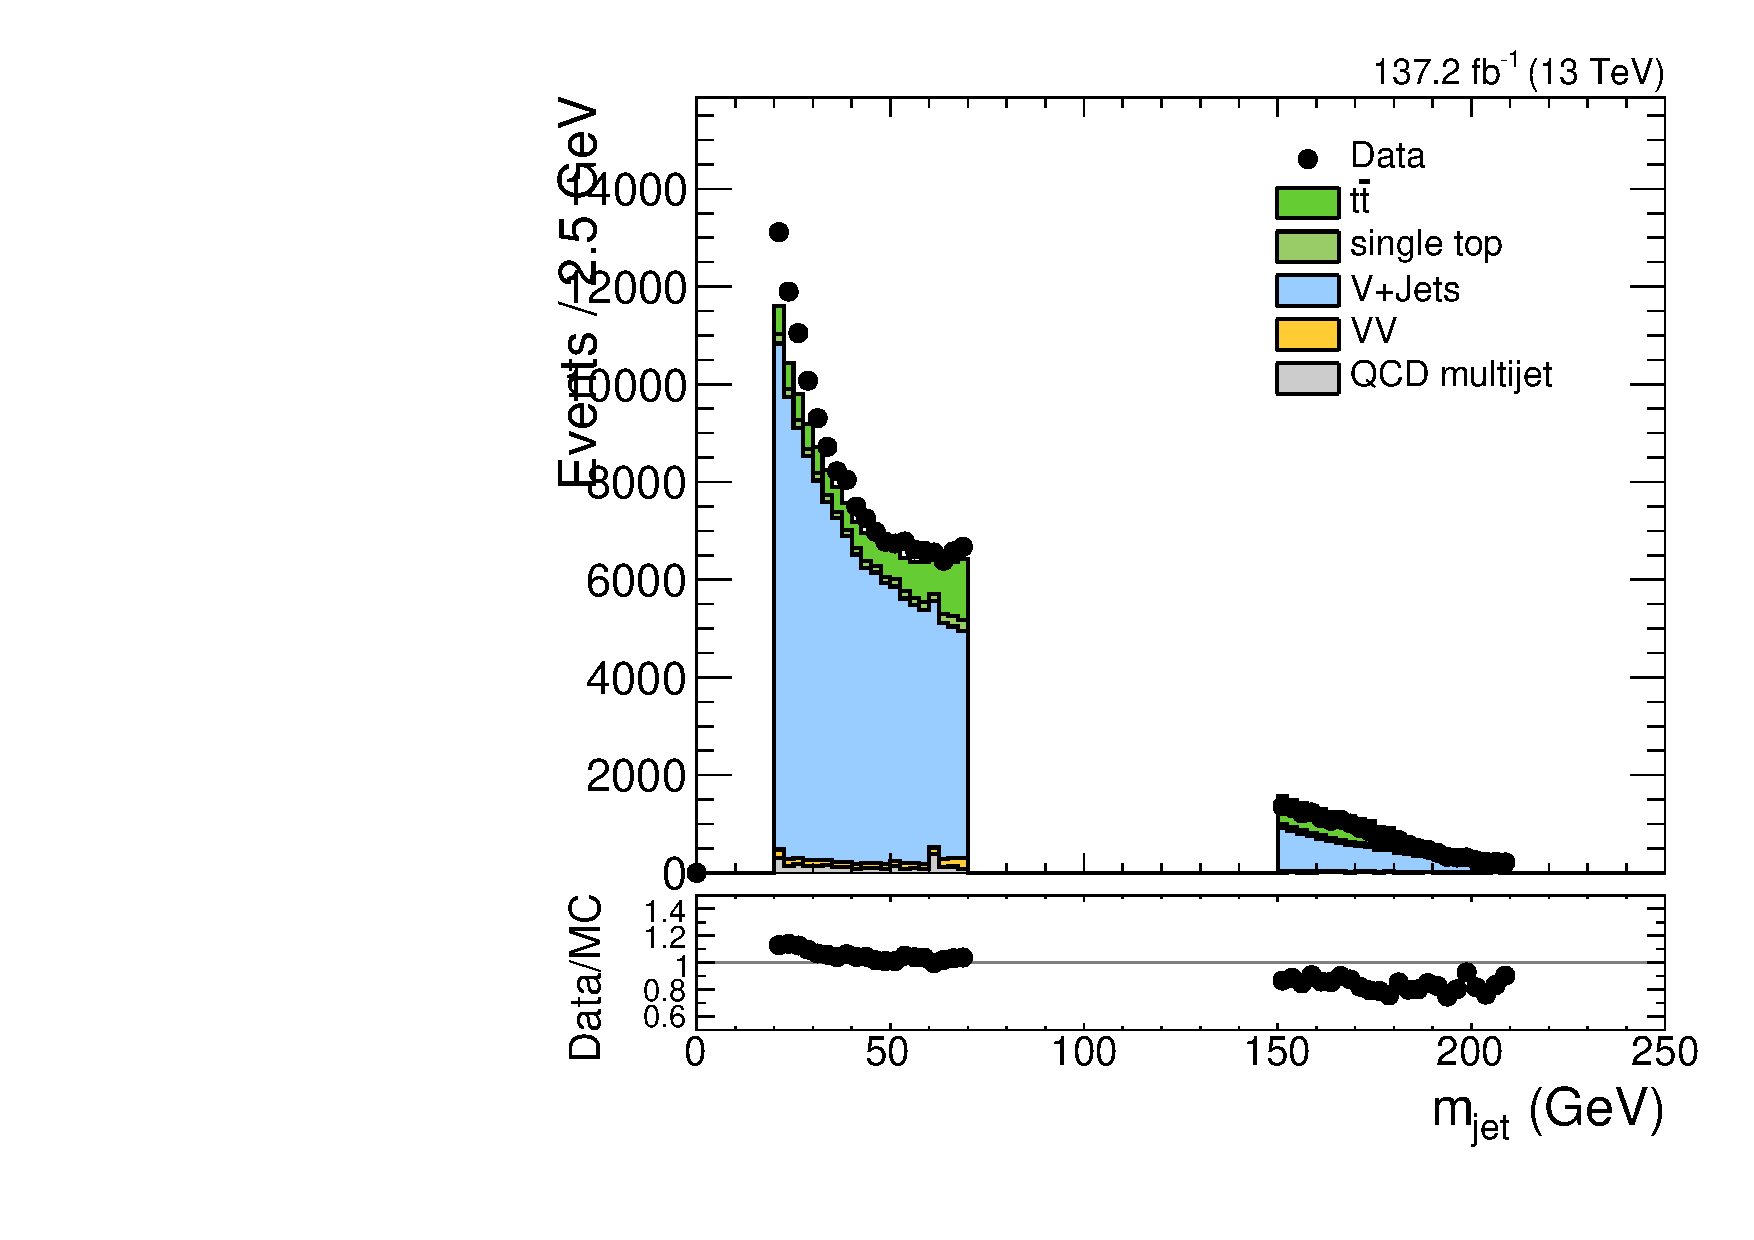
\includegraphics[width=0.4\textwidth]{fig/analysis/SB_b1_allL_allP_allC_allE_Run2_mjet.pdf}\\
  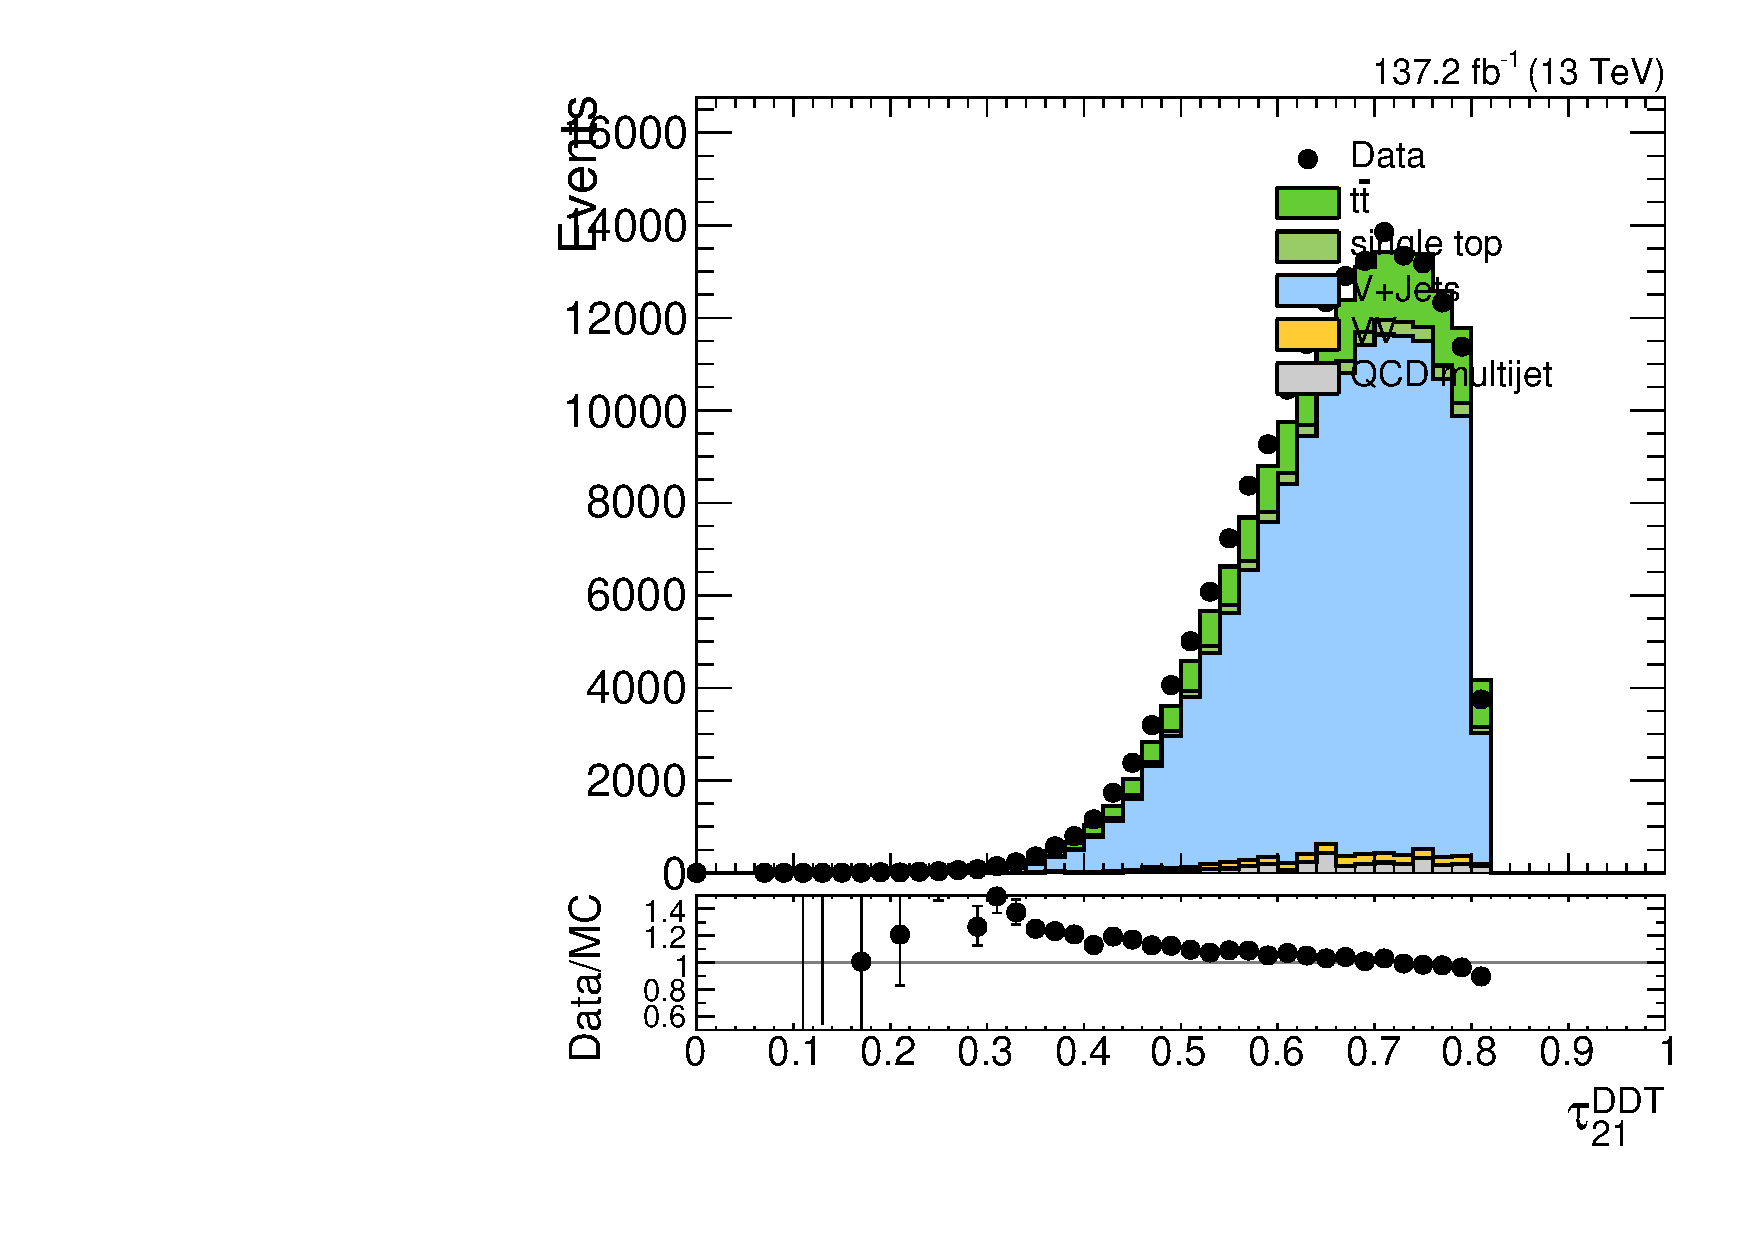
\includegraphics[width=0.4\textwidth]{fig/analysis/SB_b1_allL_allP_allC_allE_Run2_tau21DDT.pdf}
  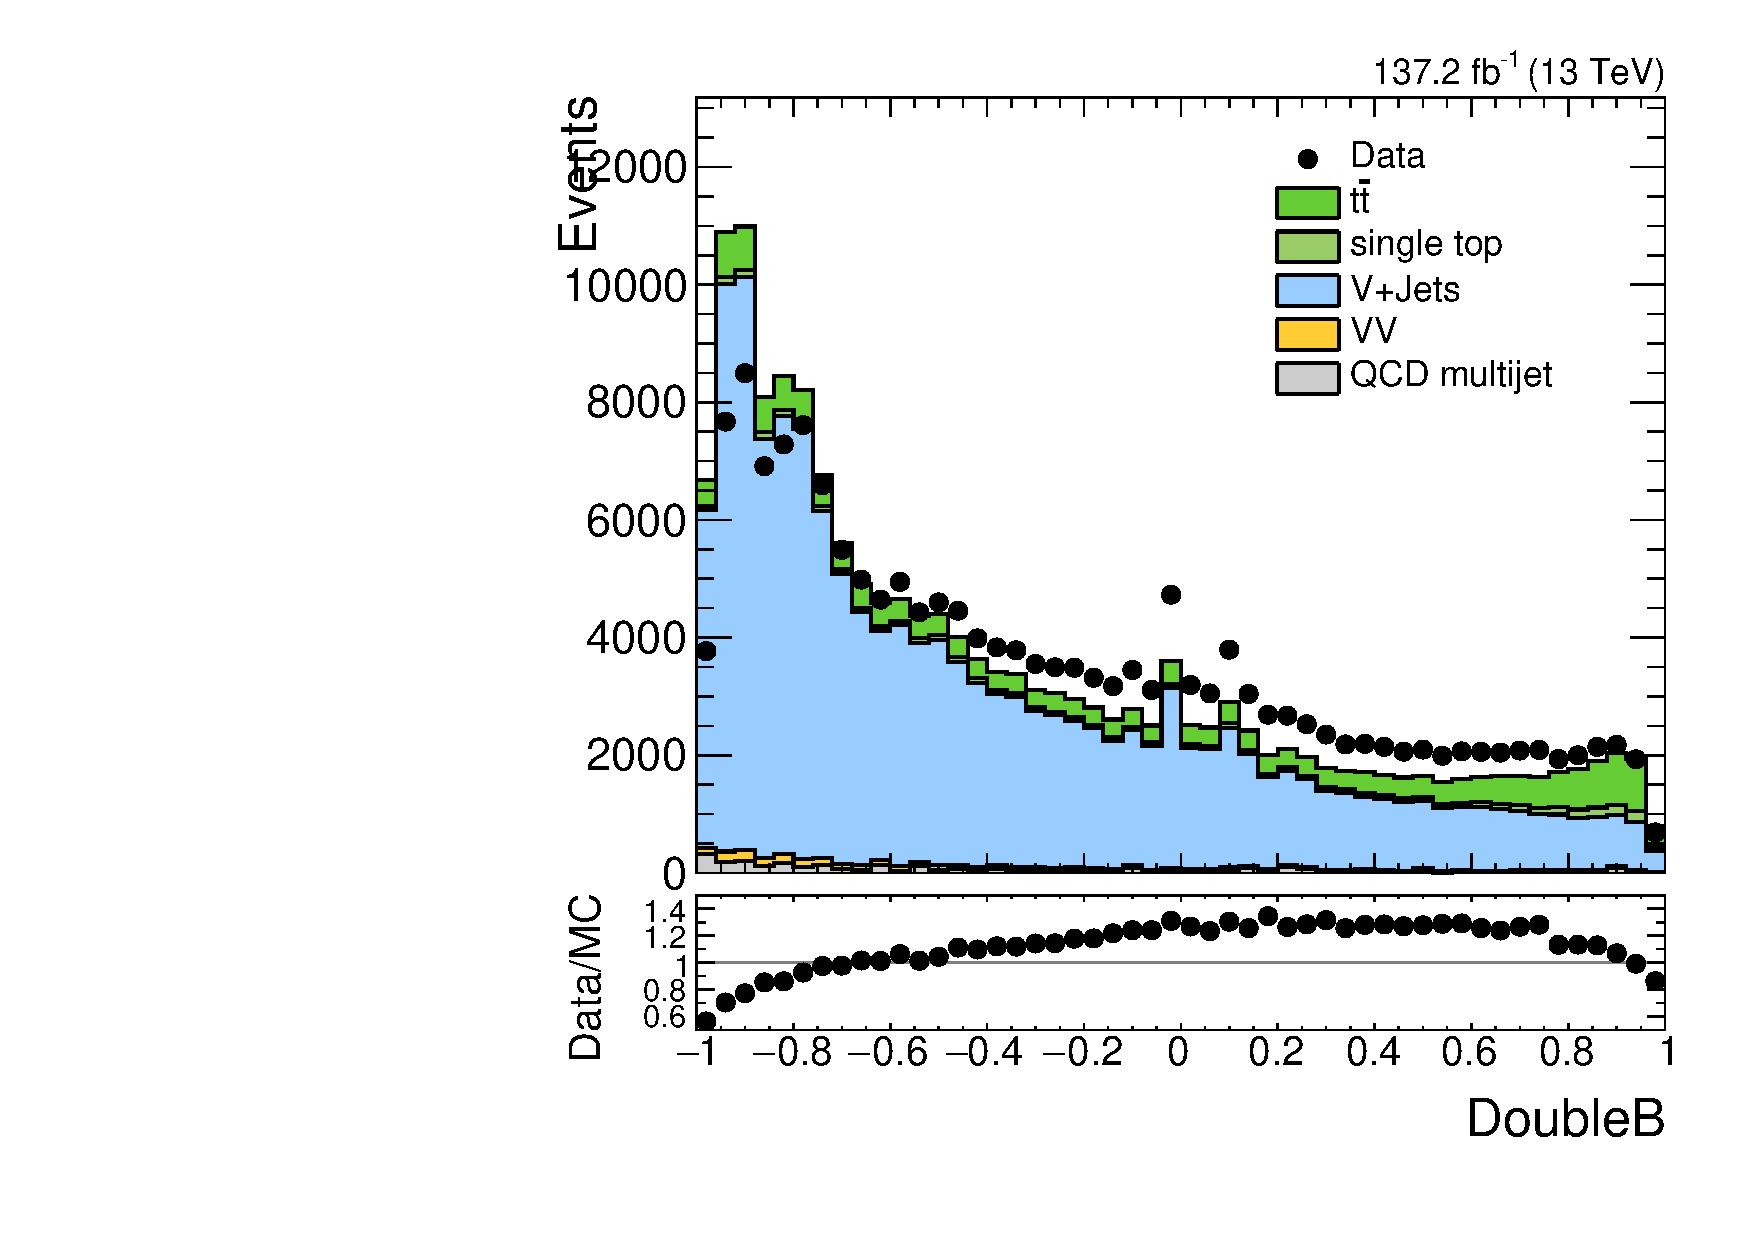
\includegraphics[width=0.4\textwidth]{fig/analysis/SB_b1_allL_allP_allC_allE_Run2_DoubleB.pdf}\\
  \caption{
    Comparison plots between data and MC from Run 2 for the \pt, $\eta$, \MJ (soft drop mass), \nsubjDDT, and \DoubleB tagger of the selected \Vhad candidate (leading AK8 jet), in the jet mass sideband.
  }
  \label{fig:SB_controlPlotsRun2_3}
\end{figure}

\begin{figure}[htbp]
  \centering
  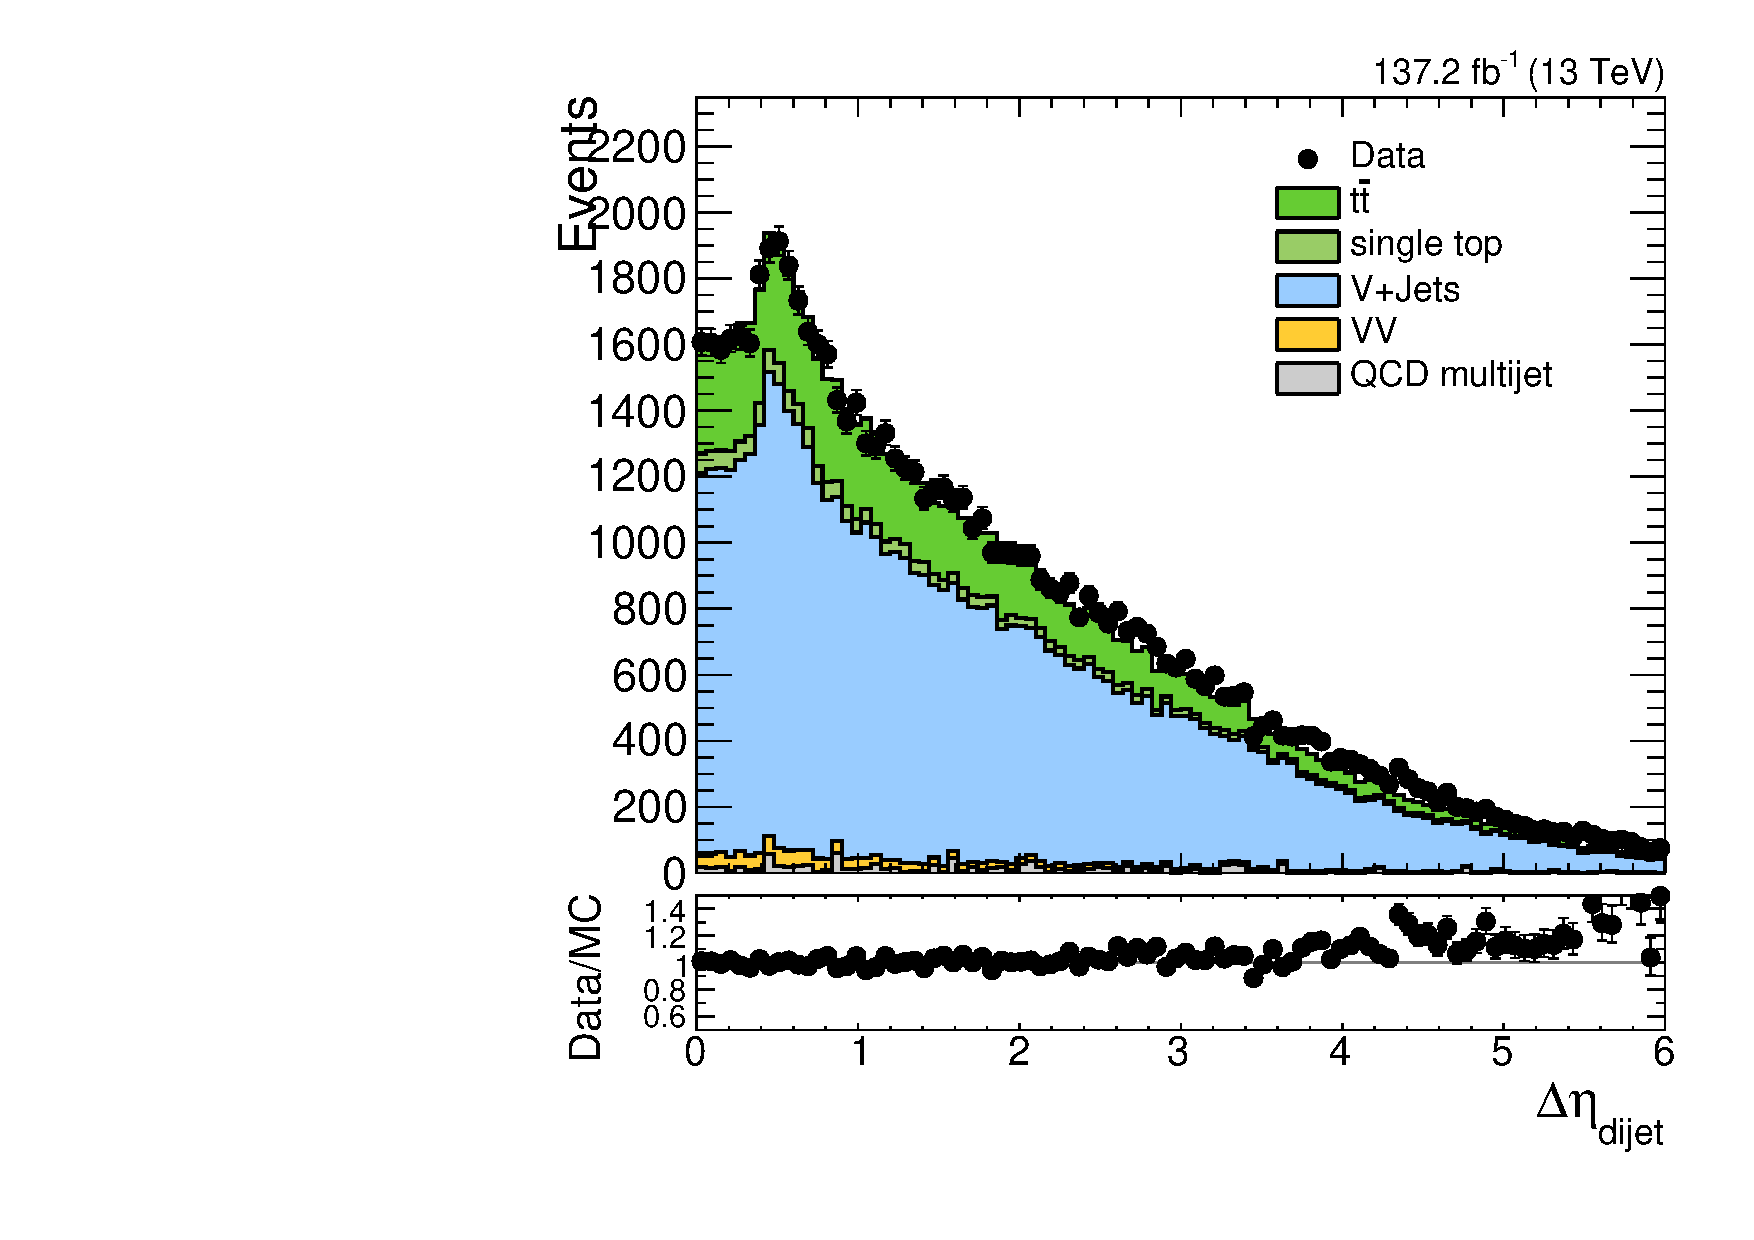
\includegraphics[width=0.4\textwidth]{fig/analysis/SB_b1_allL_allP_allC_allE_Run2_lnujj_vbfDEta.pdf}
  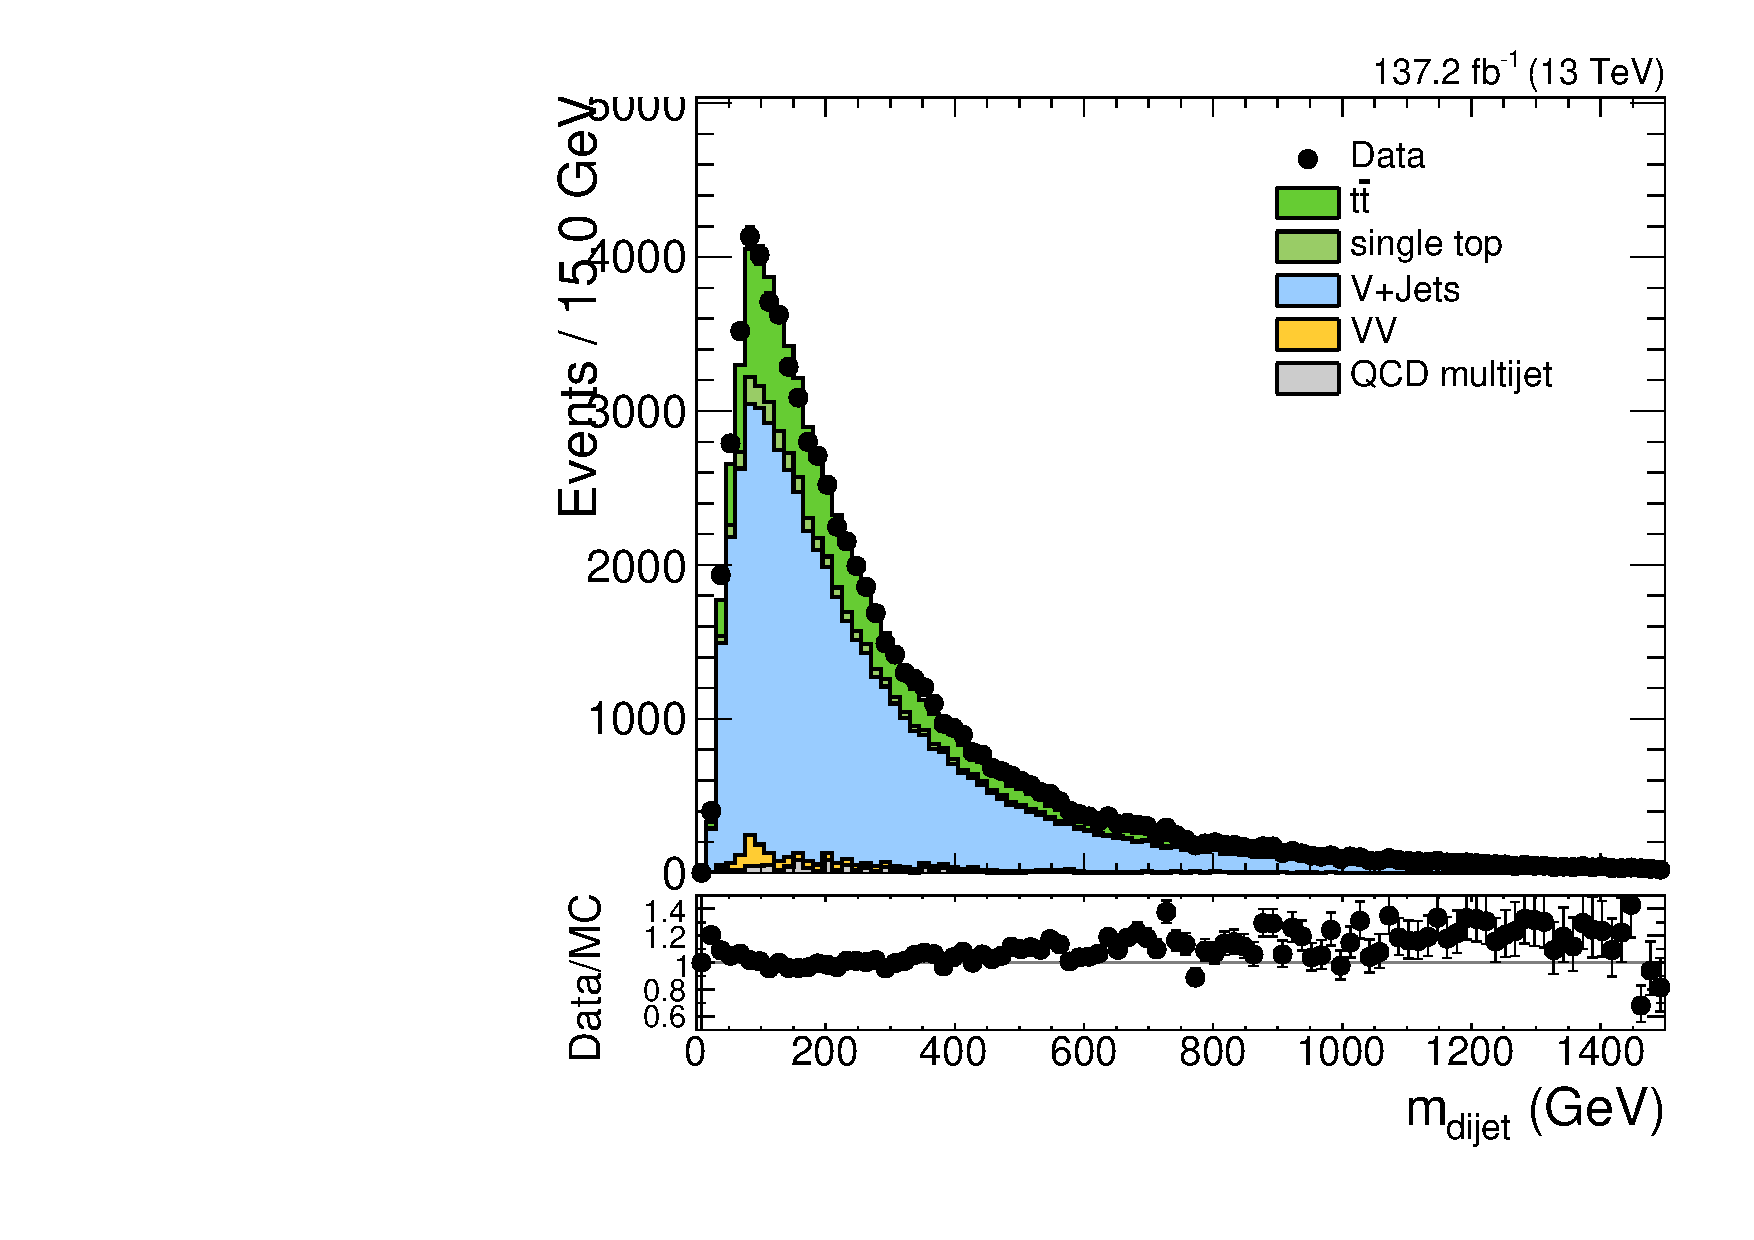
\includegraphics[width=0.4\textwidth]{fig/analysis/SB_b1_allL_allP_allC_allE_Run2_lnujj_vbfMass.pdf}\\
  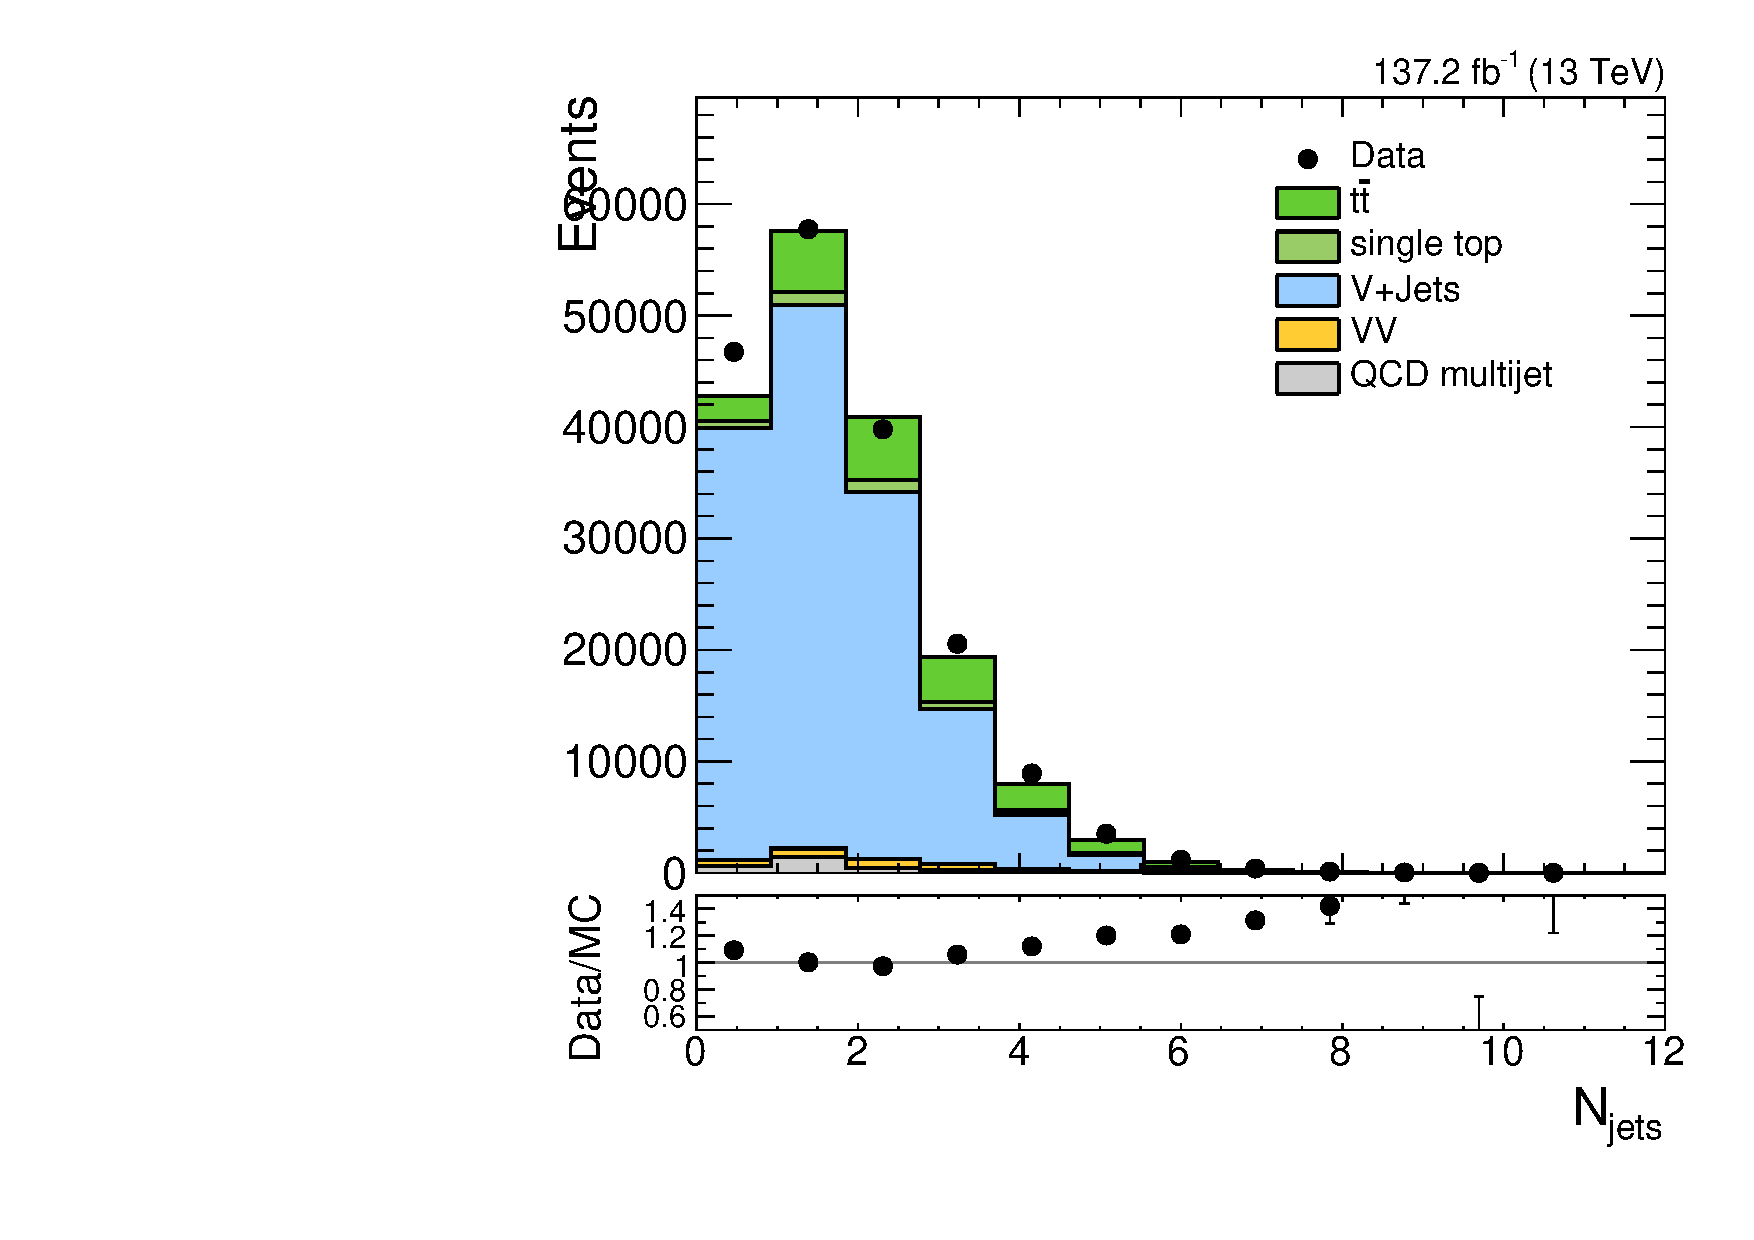
\includegraphics[width=0.4\textwidth]{fig/analysis/SB_b1_allL_allP_allC_allE_Run2_lnujj_nJets.pdf}
  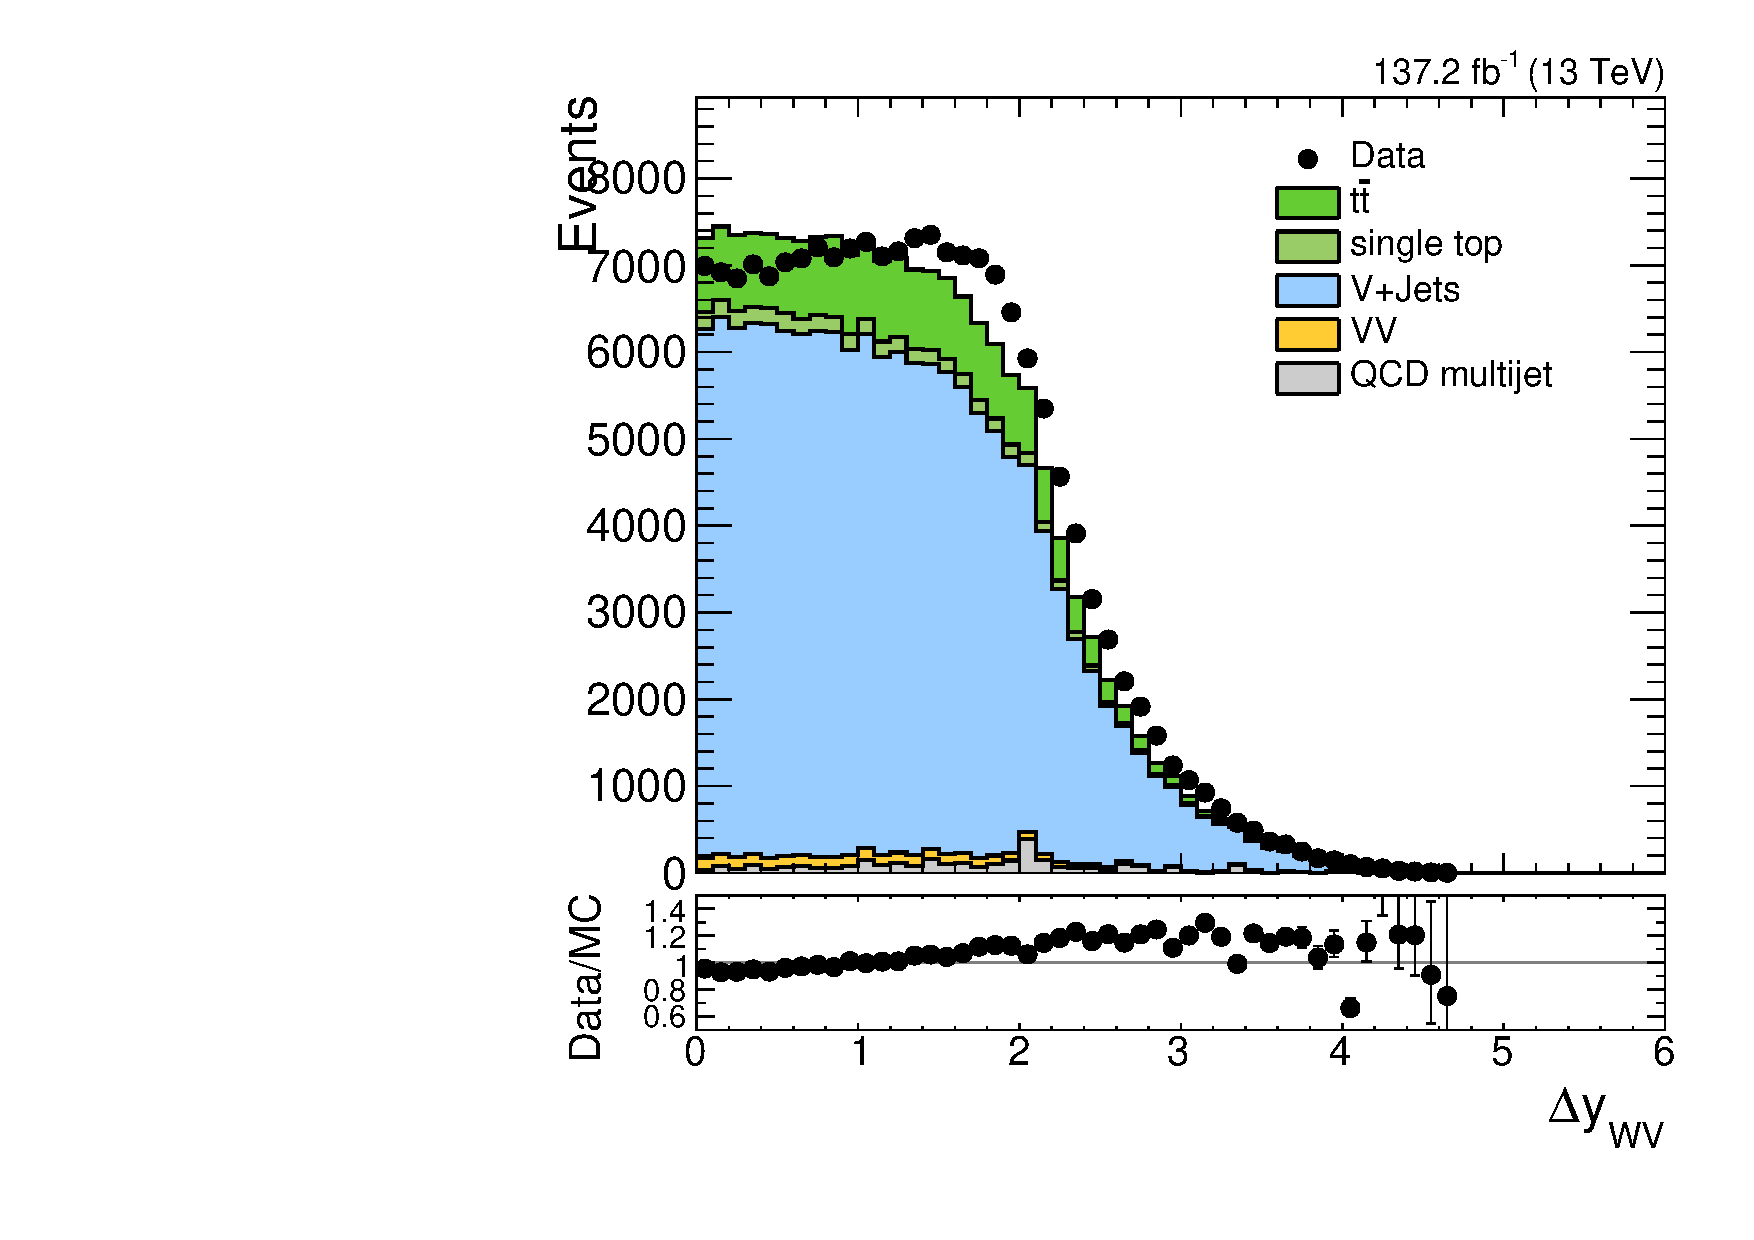
\includegraphics[width=0.4\textwidth]{fig/analysis/SB_b1_allL_allP_allC_allE_Run2_dy.pdf}\\
  \caption{
    Comparison plots between data and MC from Run 2 for the separation in $\eta$ of the \VBF forward jets, invariant mass of the \VBF jets, number of selected standard jets, and rapidity separation between the reconstructed bosons, in the jet mass sideband.
  }
  \label{fig:SB_controlPlotsRun2_4}
\end{figure}

\subsubsection{Control Plots in the Top-Enriched Control Region}

% Top-enriched control plots
Figure~\ref{fig:CR_controlPlotsRun2_1} shows control plots of lepton-related observables in the top-enriched control region, with the lepton \pt, $\eta$, and \Etmiss in both the $e$ and $\mu$ channels.
For figure~\ref{fig:CR_controlPlotsRun2_2}, the distributions of the \Wlep \pt, transverse mass, and \MVV are shown, for both the $e$ and $\mu$ channels.
In figure~\ref{fig:CR_controlPlotsRun2_3}, distributions of variables related to the \Vhad jet are shown, with the jet \pt, $\eta$, \MJ, \nsubjDDT, and \DoubleB tagger.
Finally, in figure~\ref{fig:CR_controlPlotsRun2_4}, \VBF-related distributions are shown for \DetaVBF, \mjjVBF, \nJets, and \Dy.

\begin{figure}[htbp]
  \centering
  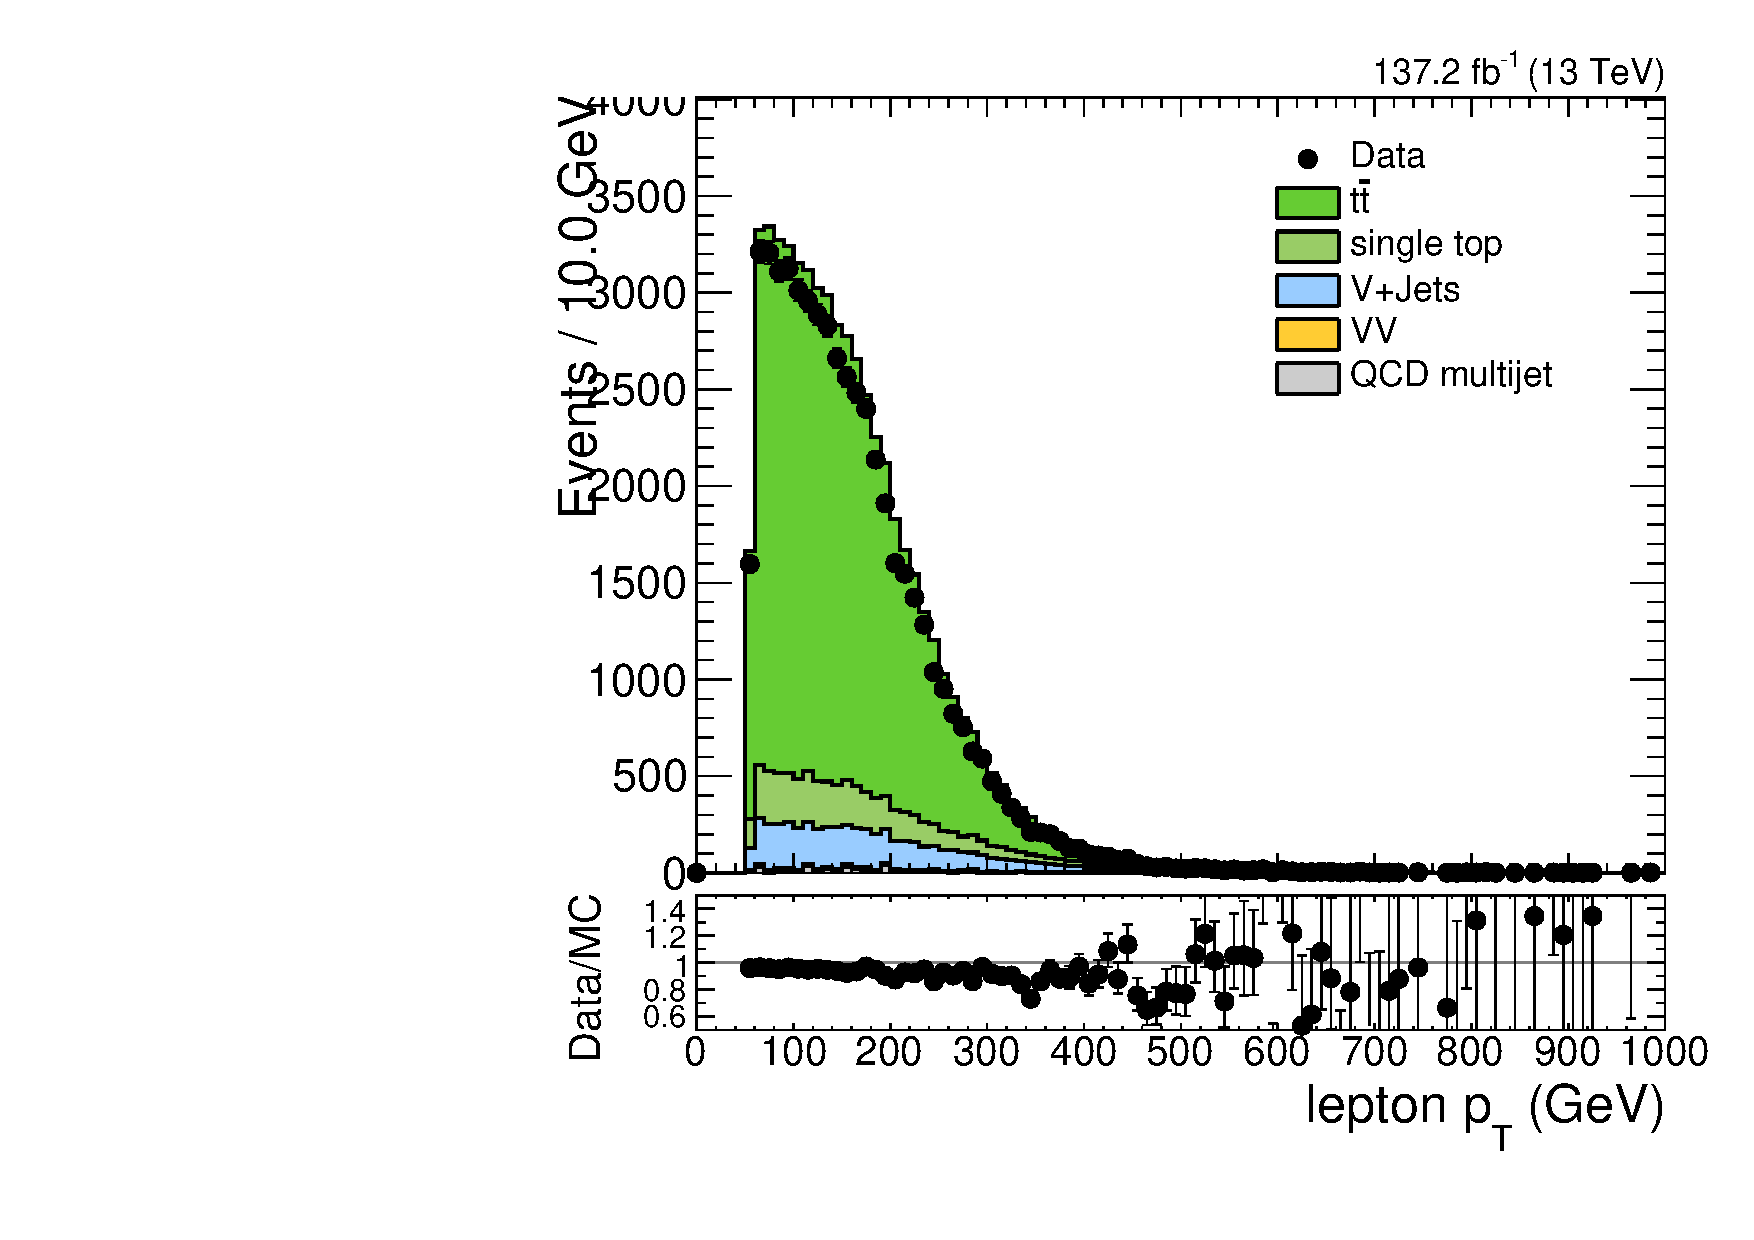
\includegraphics[width=0.4\textwidth]{fig/analysis/CR_b1_mu_allP_allC_allE_Run2_lnujj_l1_l_pt.pdf}
  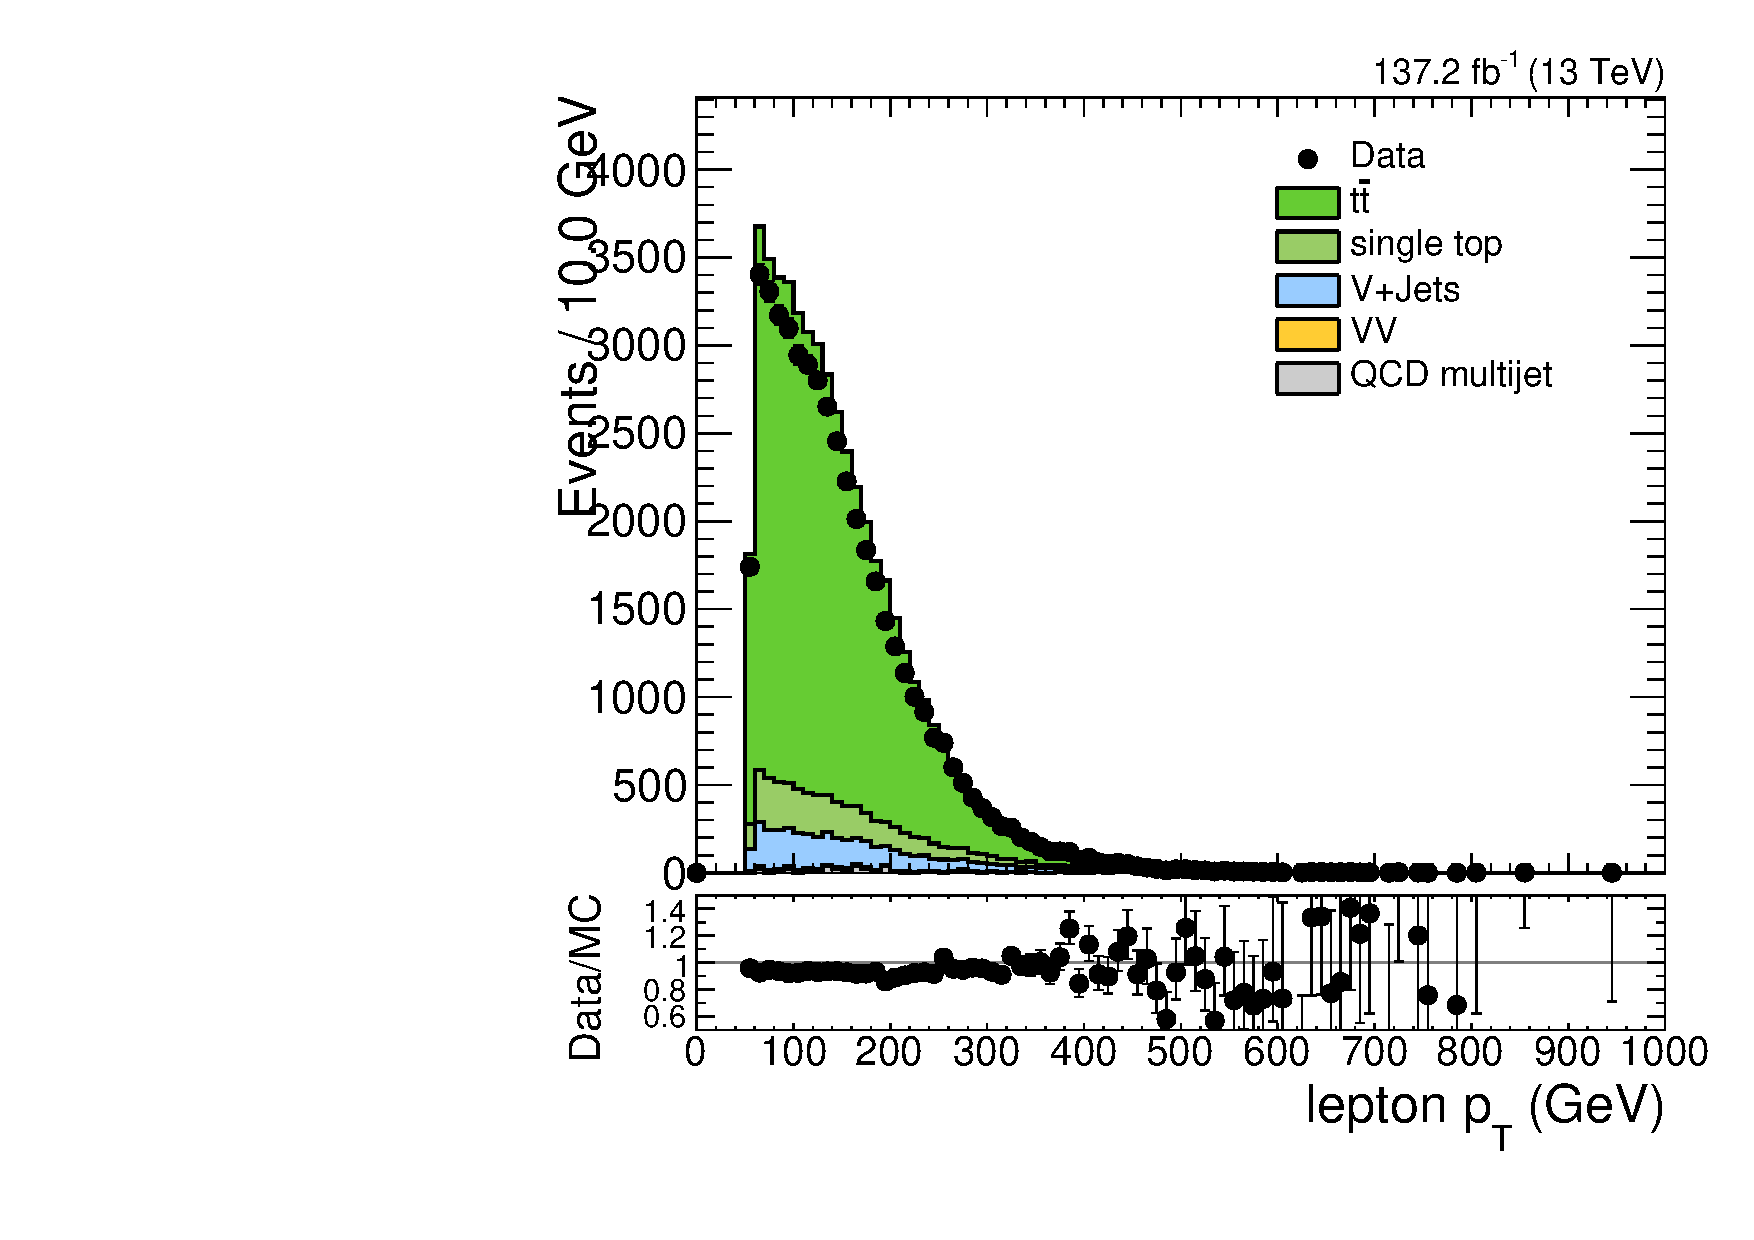
\includegraphics[width=0.4\textwidth]{fig/analysis/CR_b1_e_allP_allC_allE_Run2_lnujj_l1_l_pt.pdf}\\
  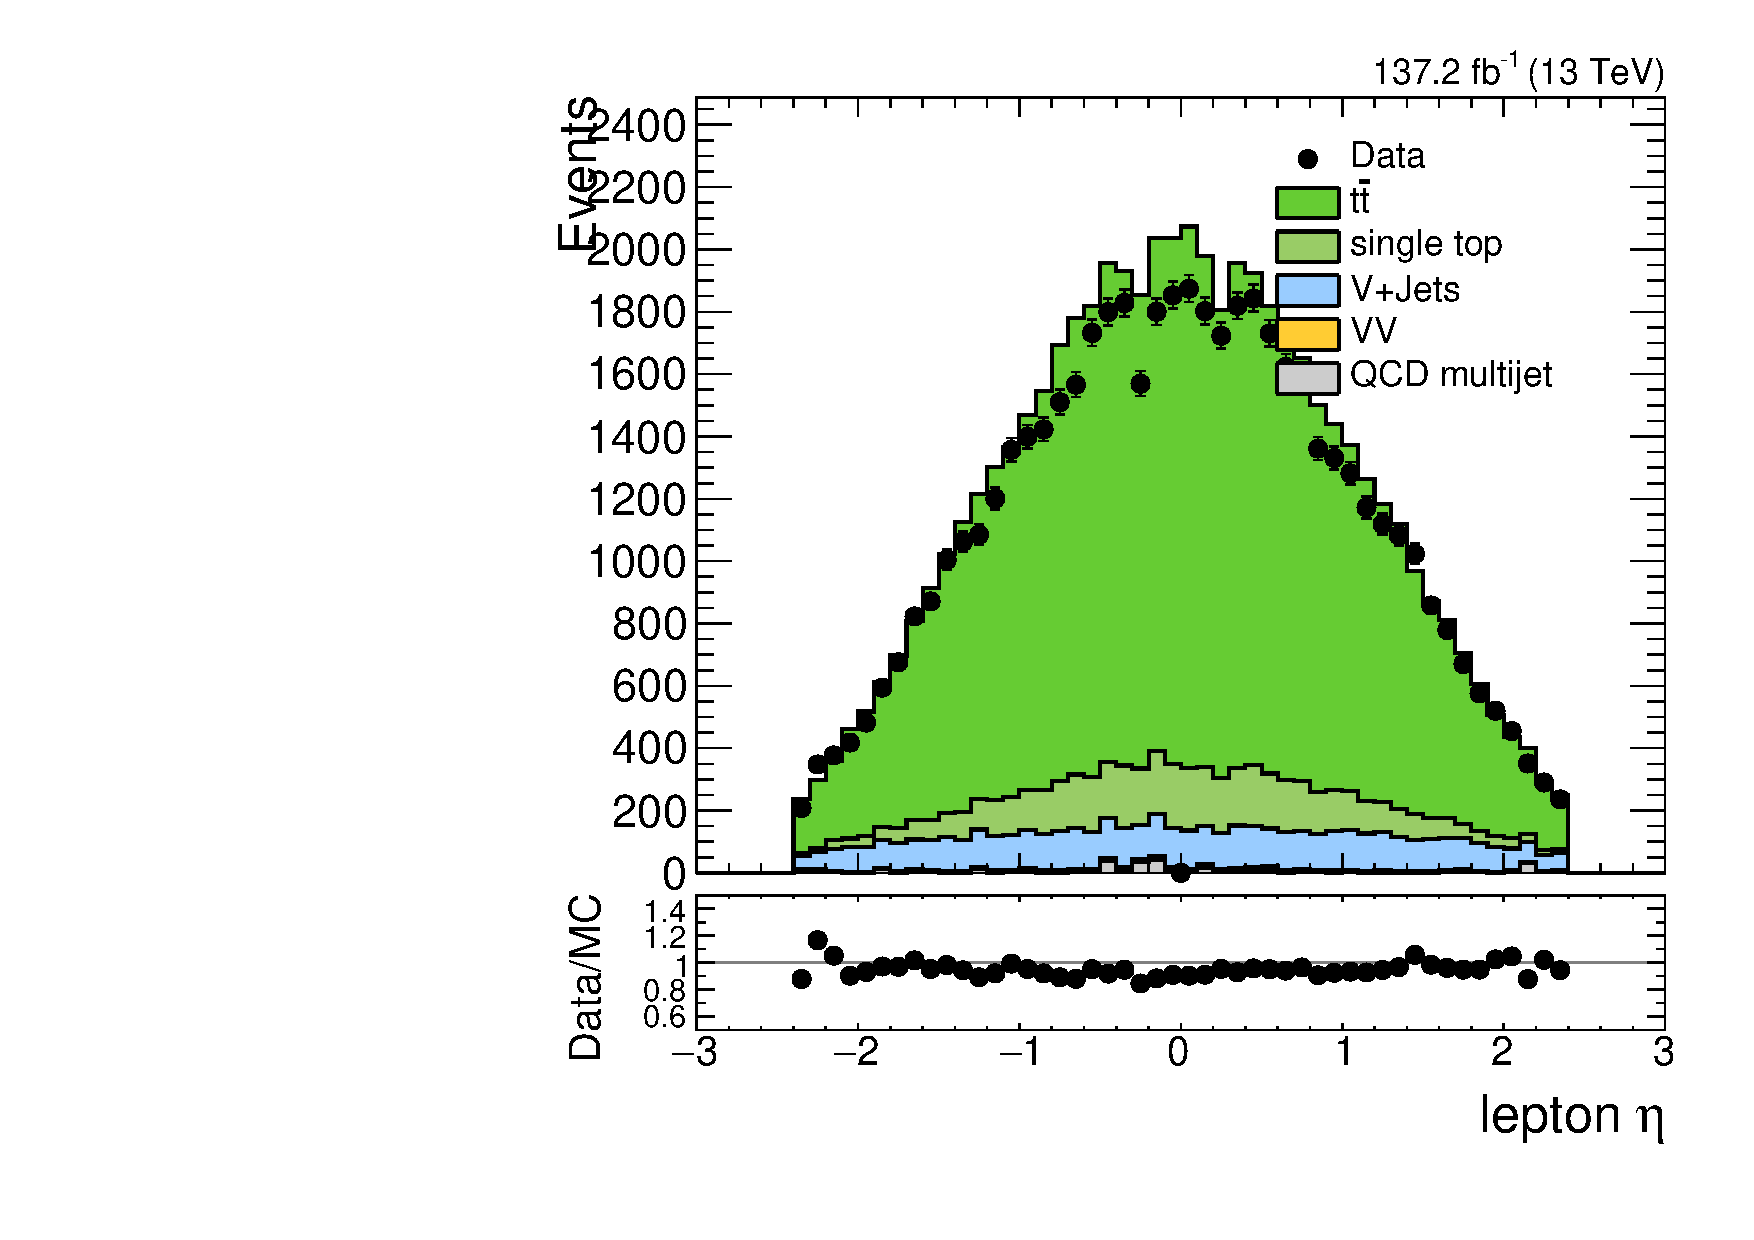
\includegraphics[width=0.4\textwidth]{fig/analysis/CR_b1_mu_allP_allC_allE_Run2_lnujj_l1_l_eta.pdf}
  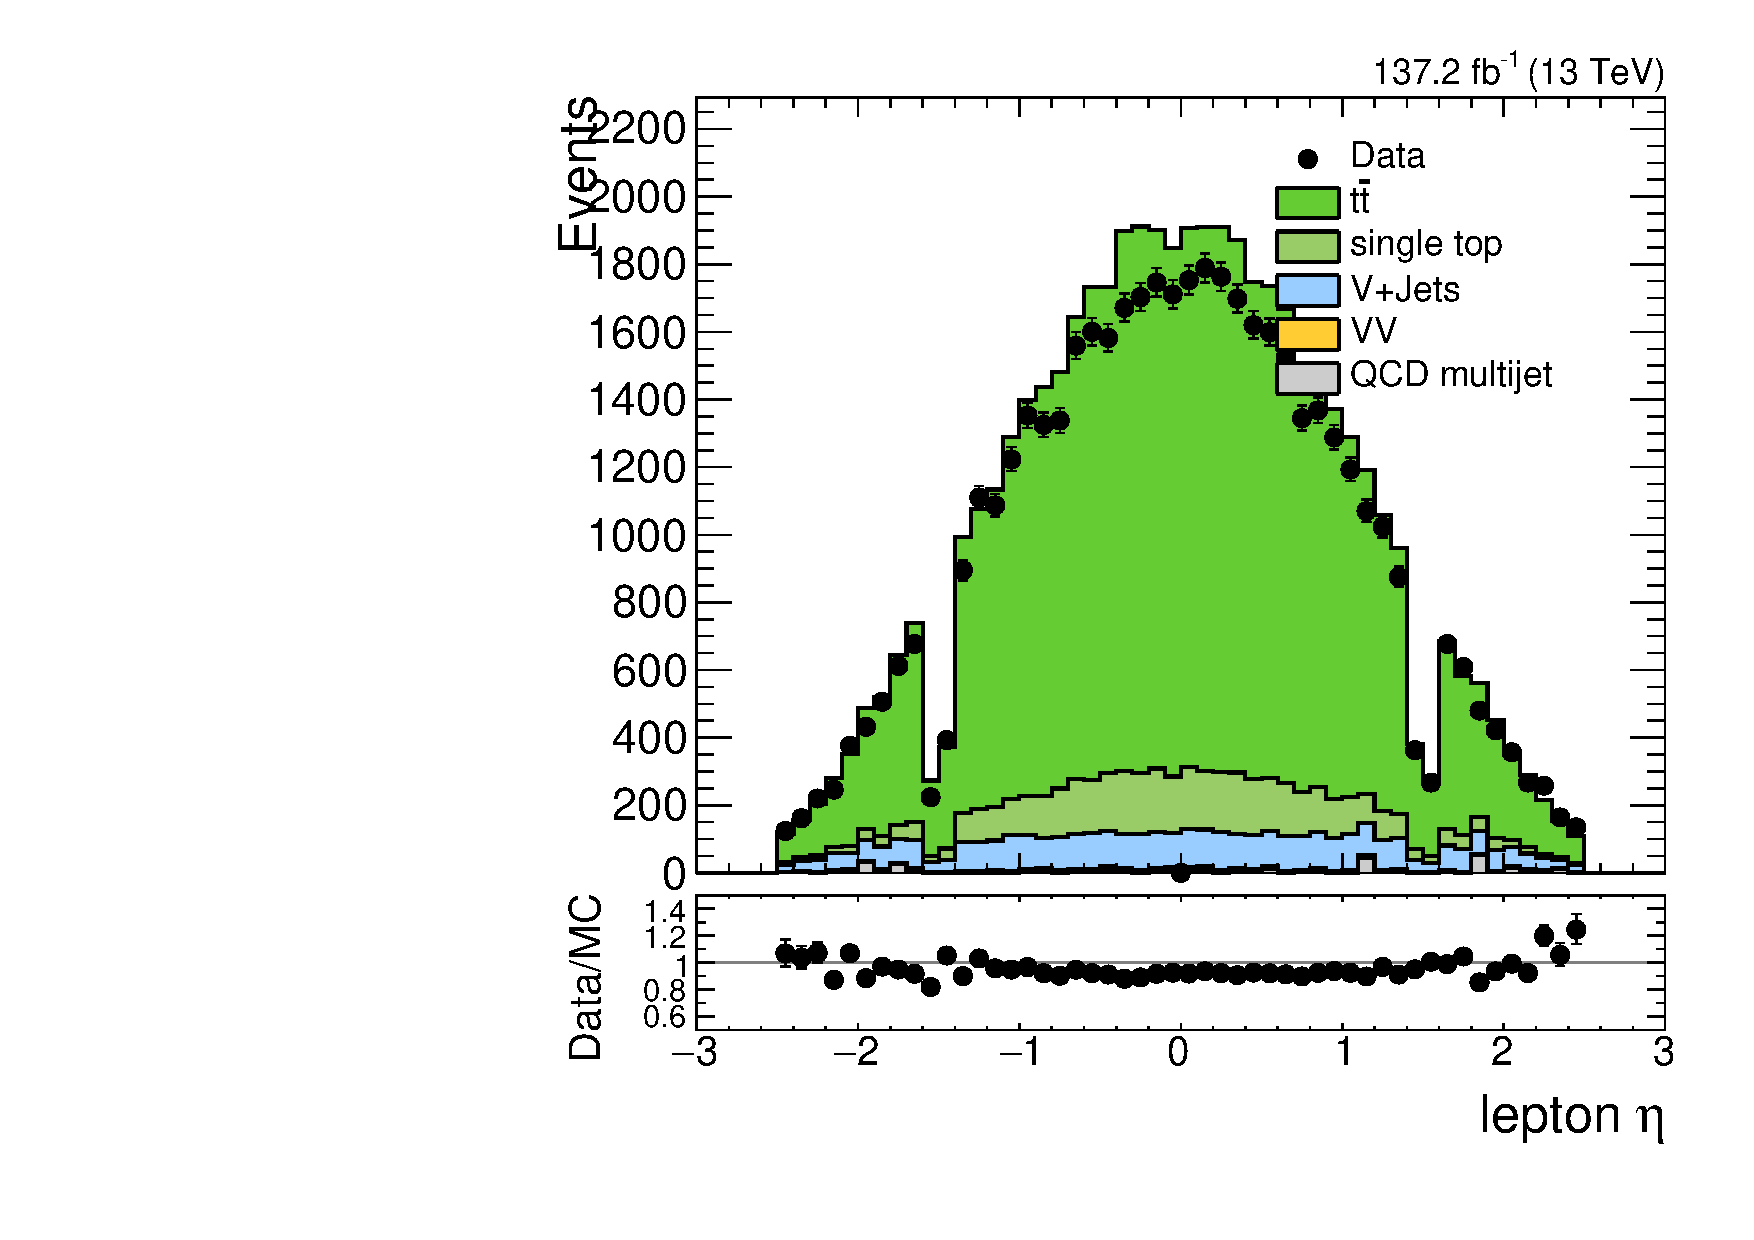
\includegraphics[width=0.4\textwidth]{fig/analysis/CR_b1_e_allP_allC_allE_Run2_lnujj_l1_l_eta.pdf}\\
  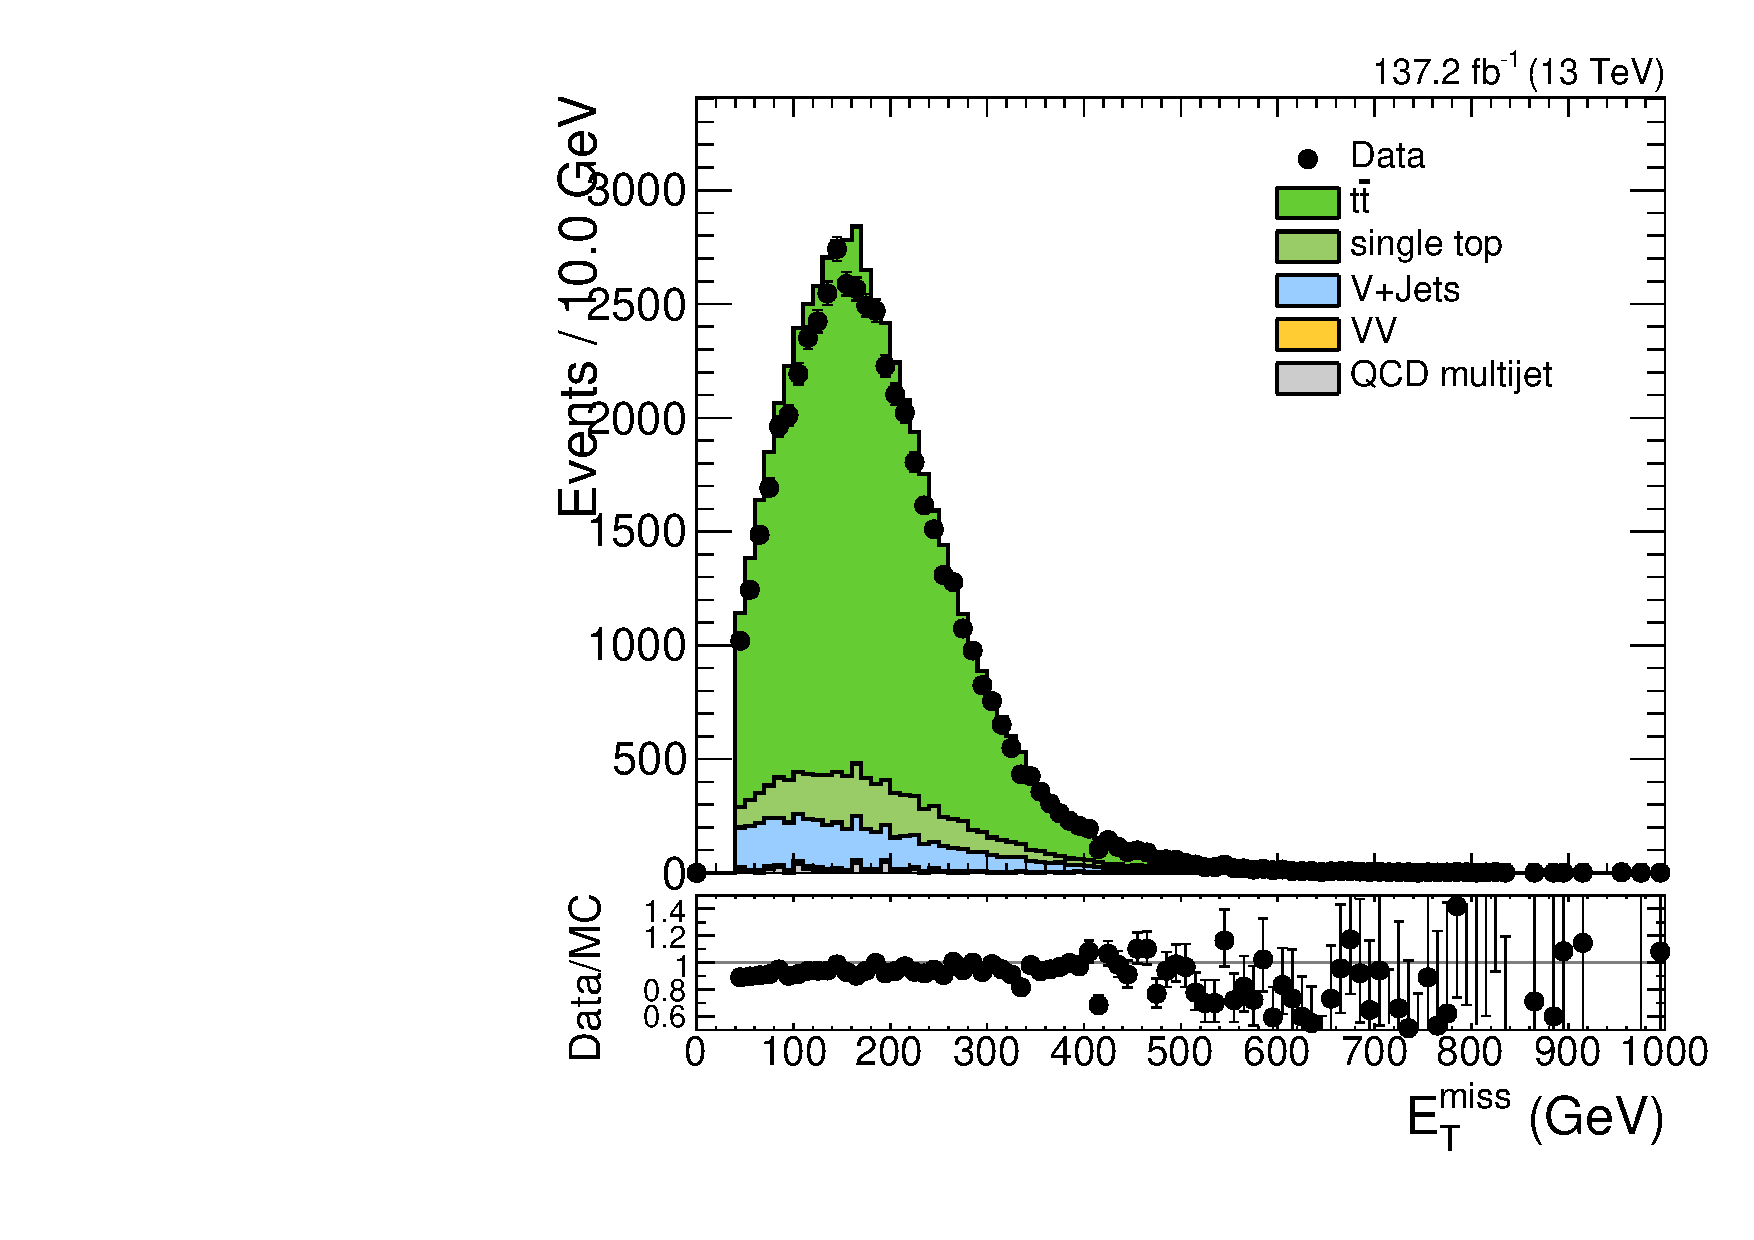
\includegraphics[width=0.4\textwidth]{fig/analysis/CR_b1_mu_allP_allC_allE_Run2_met_pt.pdf}
  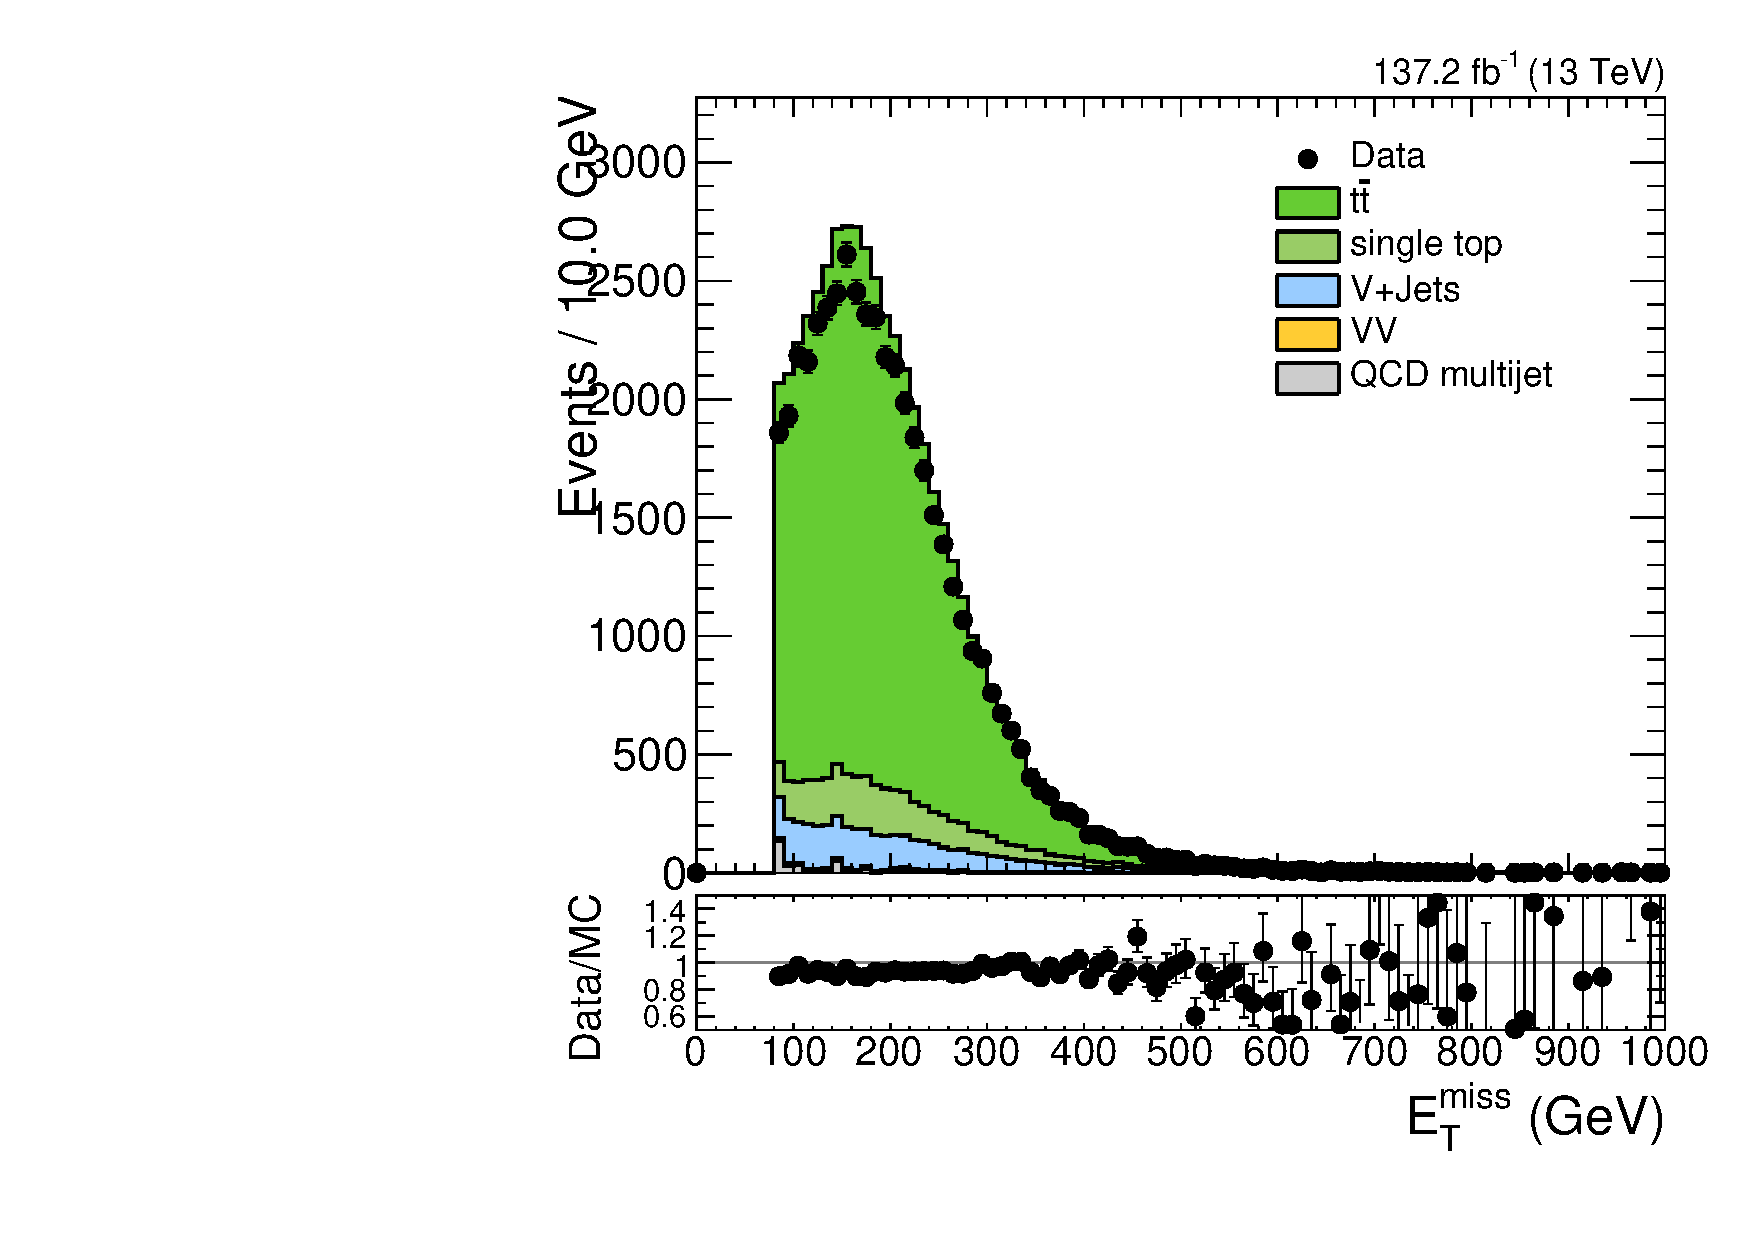
\includegraphics[width=0.4\textwidth]{fig/analysis/CR_b1_e_allP_allC_allE_Run2_met_pt.pdf}\\
  \caption{
    Comparison plots between data and MC from Run 2 for different \Wlep-related observables, in the top-enriched control region.
    From top to bottom: lepton \pt, lepton $\eta$, \Etmiss.
    Left: muon channel, right: electron channel.
  }
  \label{fig:CR_controlPlotsRun2_1}
\end{figure}

\begin{figure}[htbp]
  \centering
  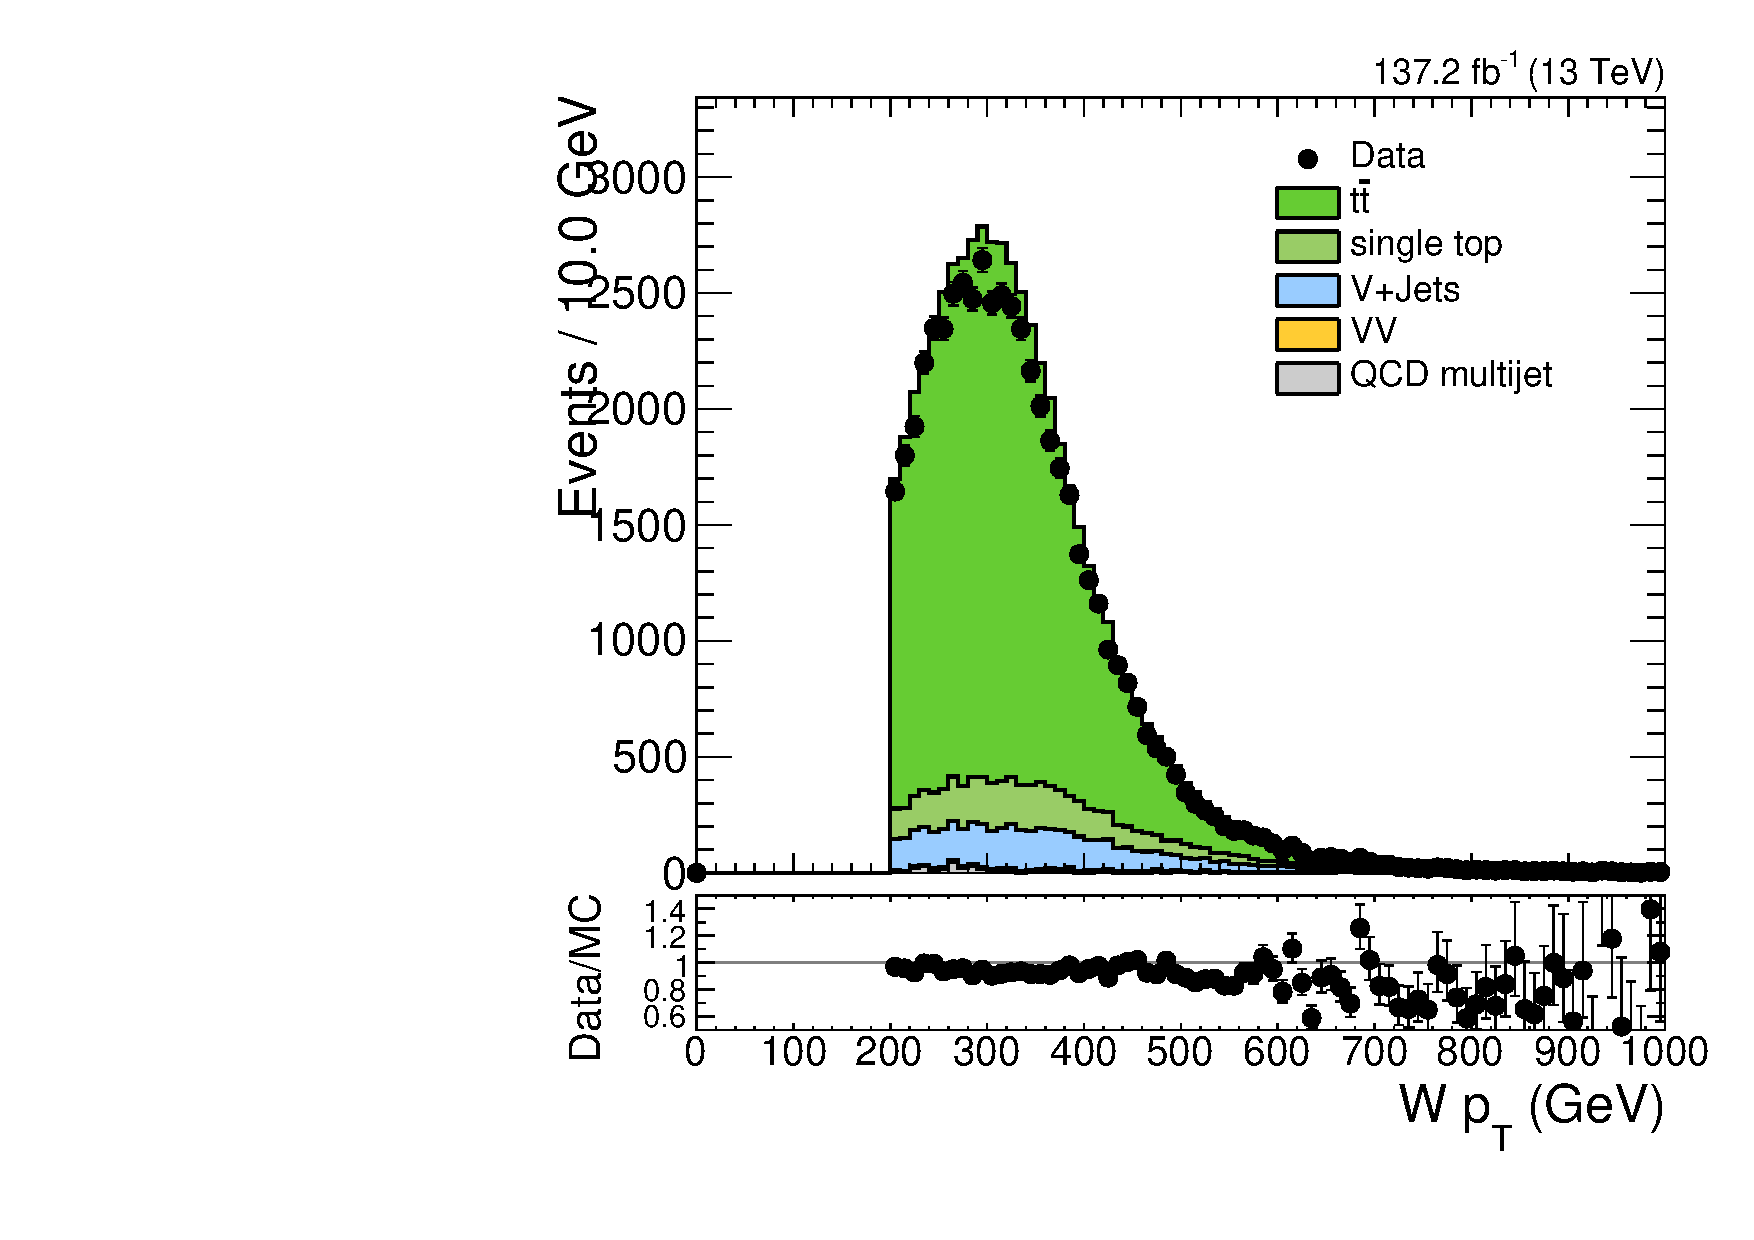
\includegraphics[width=0.4\textwidth]{fig/analysis/CR_b1_mu_allP_allC_allE_Run2_lnujj_l1_pt.pdf}
  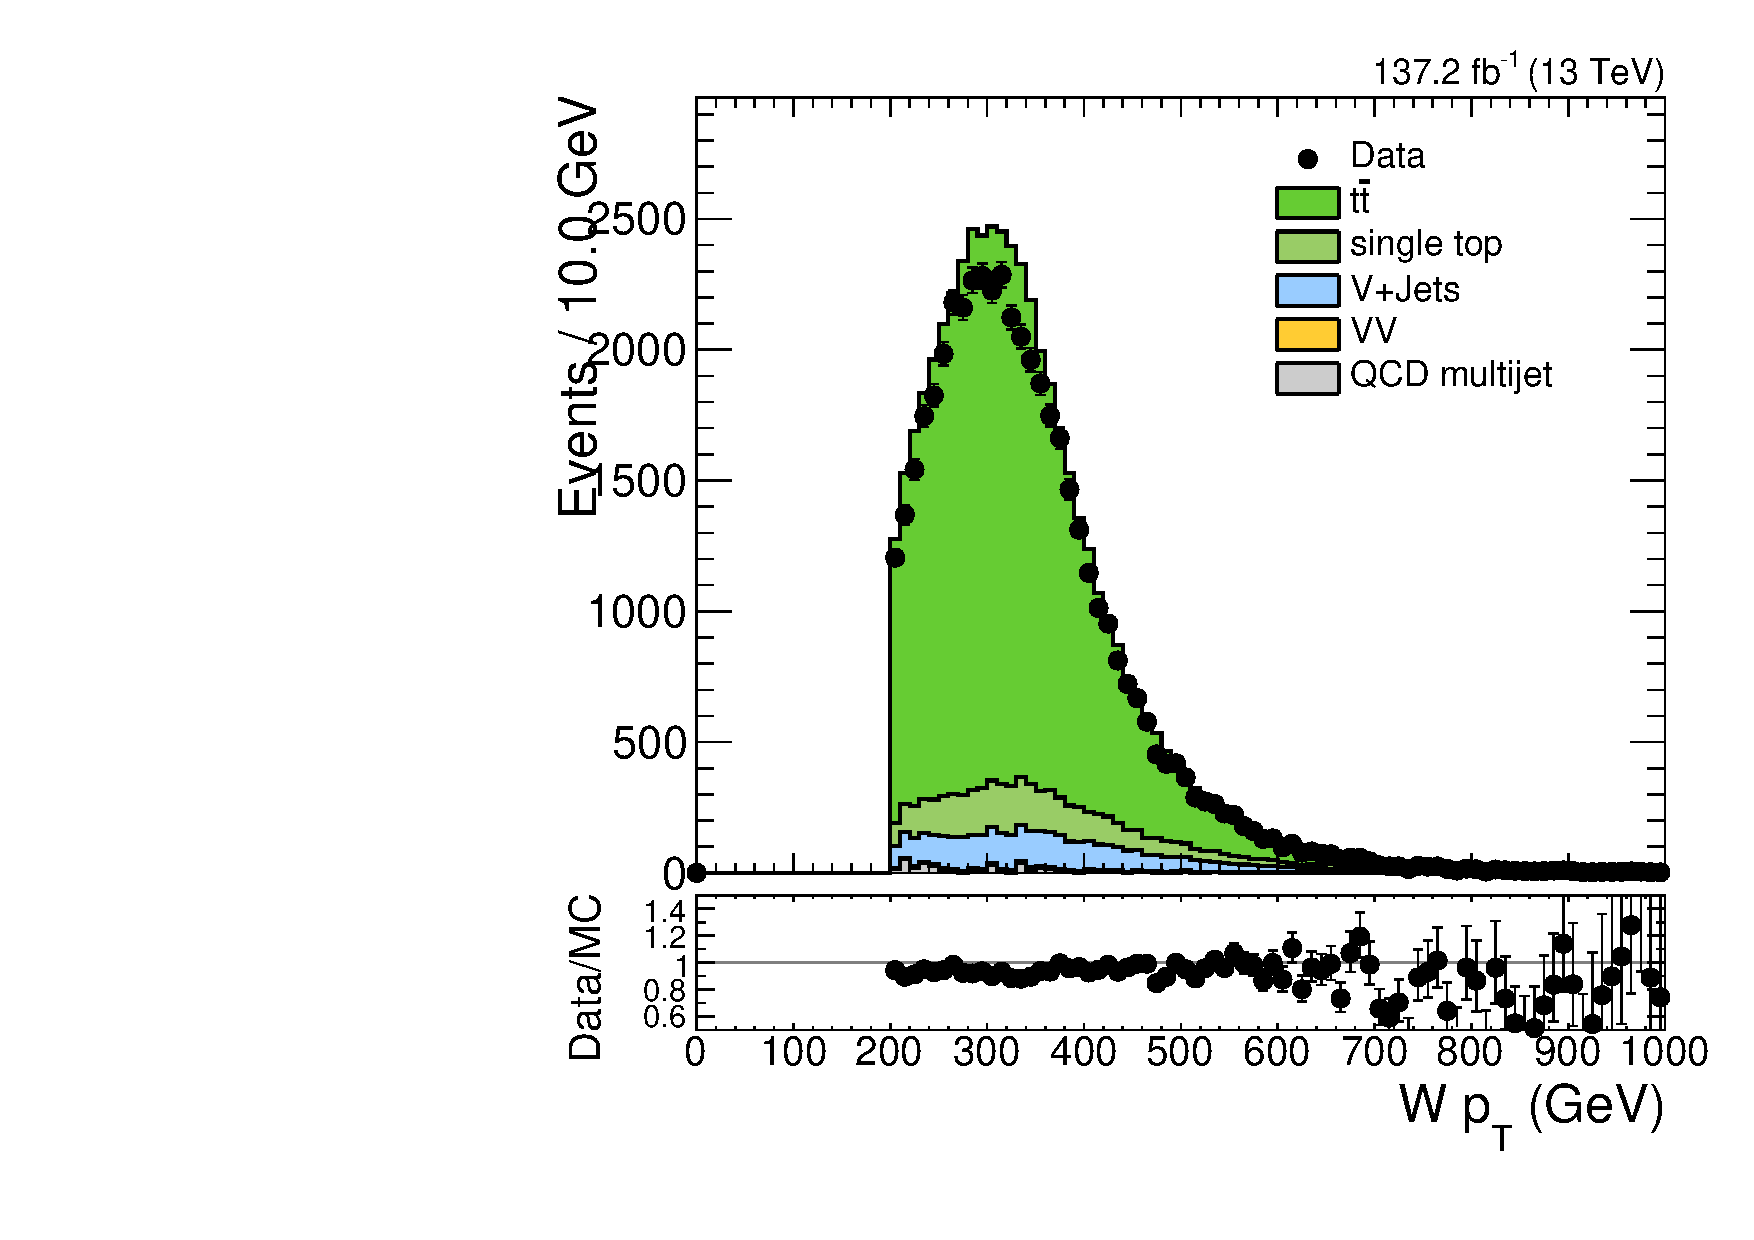
\includegraphics[width=0.4\textwidth]{fig/analysis/CR_b1_e_allP_allC_allE_Run2_lnujj_l1_pt.pdf}\\
  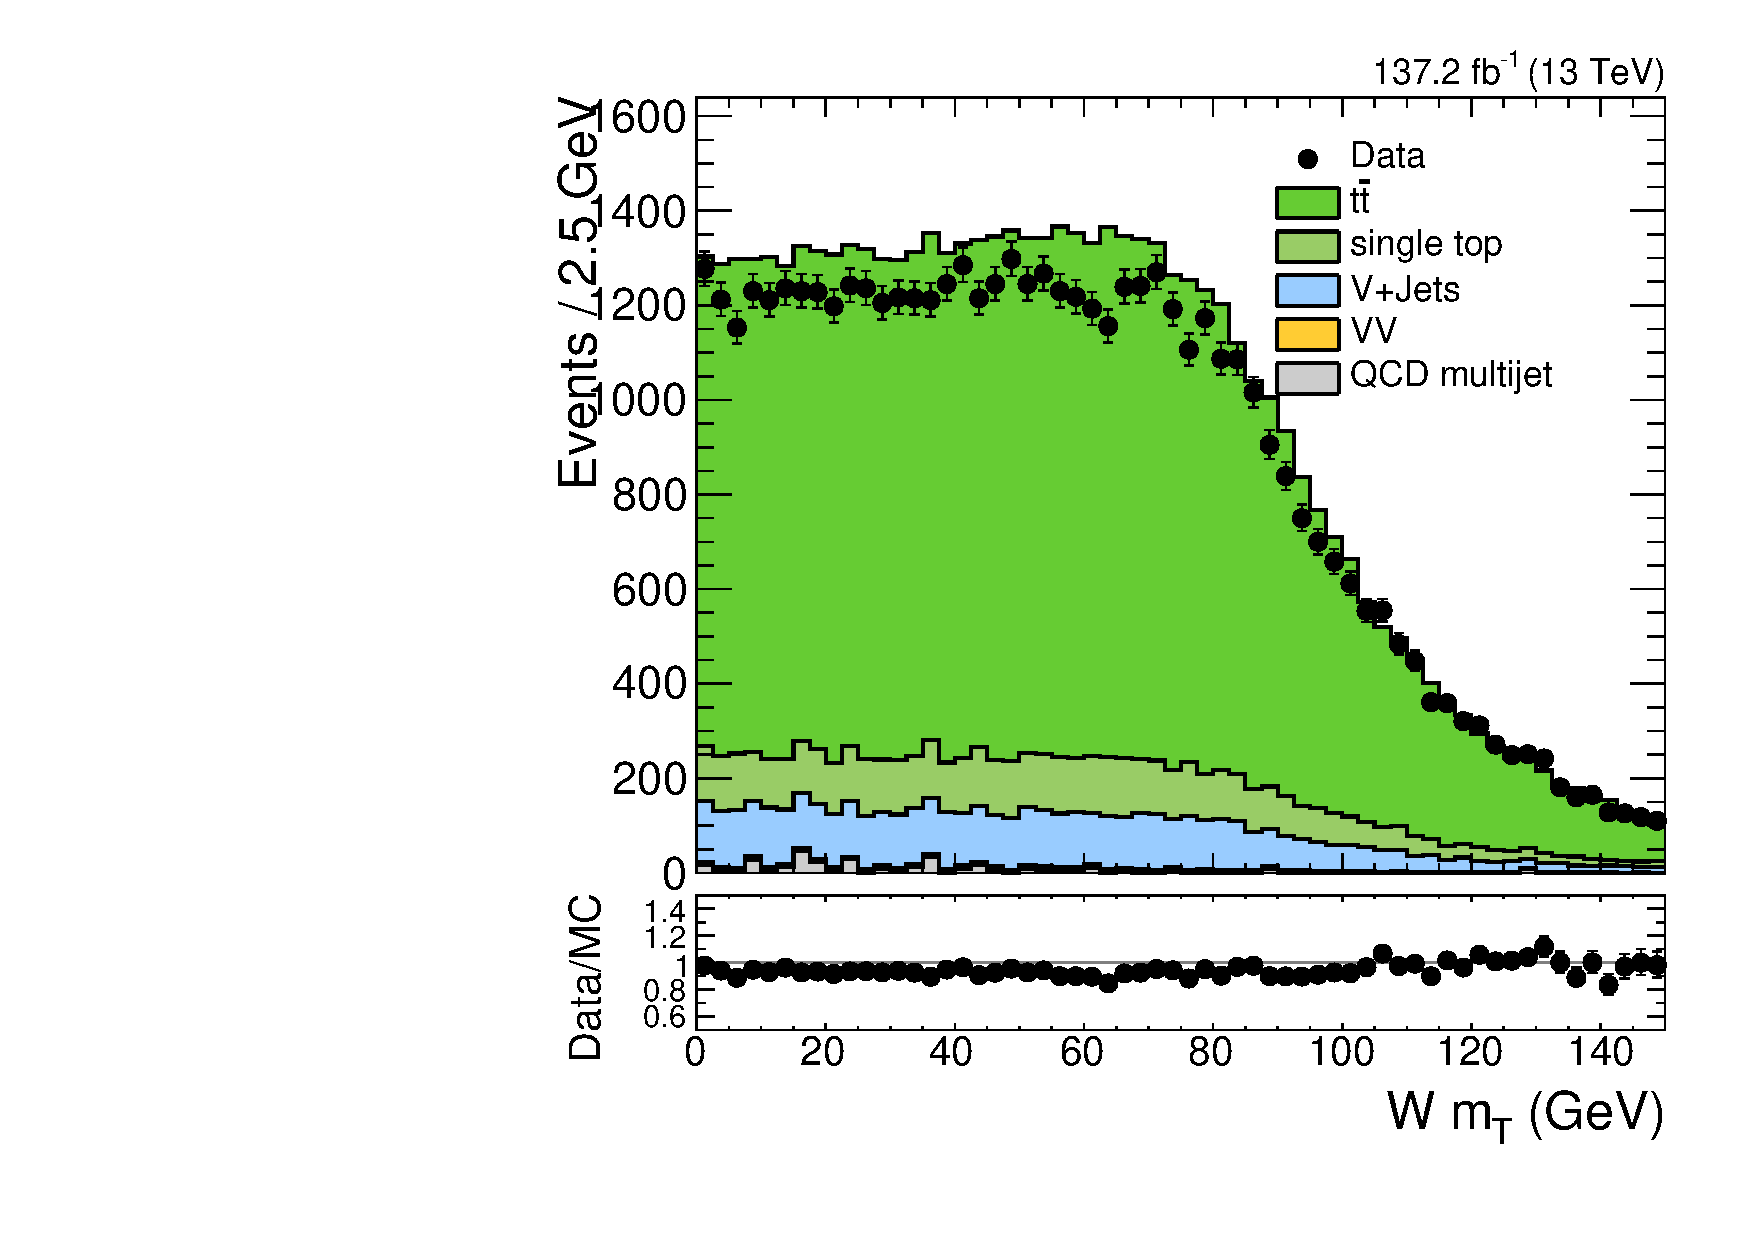
\includegraphics[width=0.4\textwidth]{fig/analysis/CR_b1_mu_allP_allC_allE_Run2_lnujj_l1_mt.pdf}
  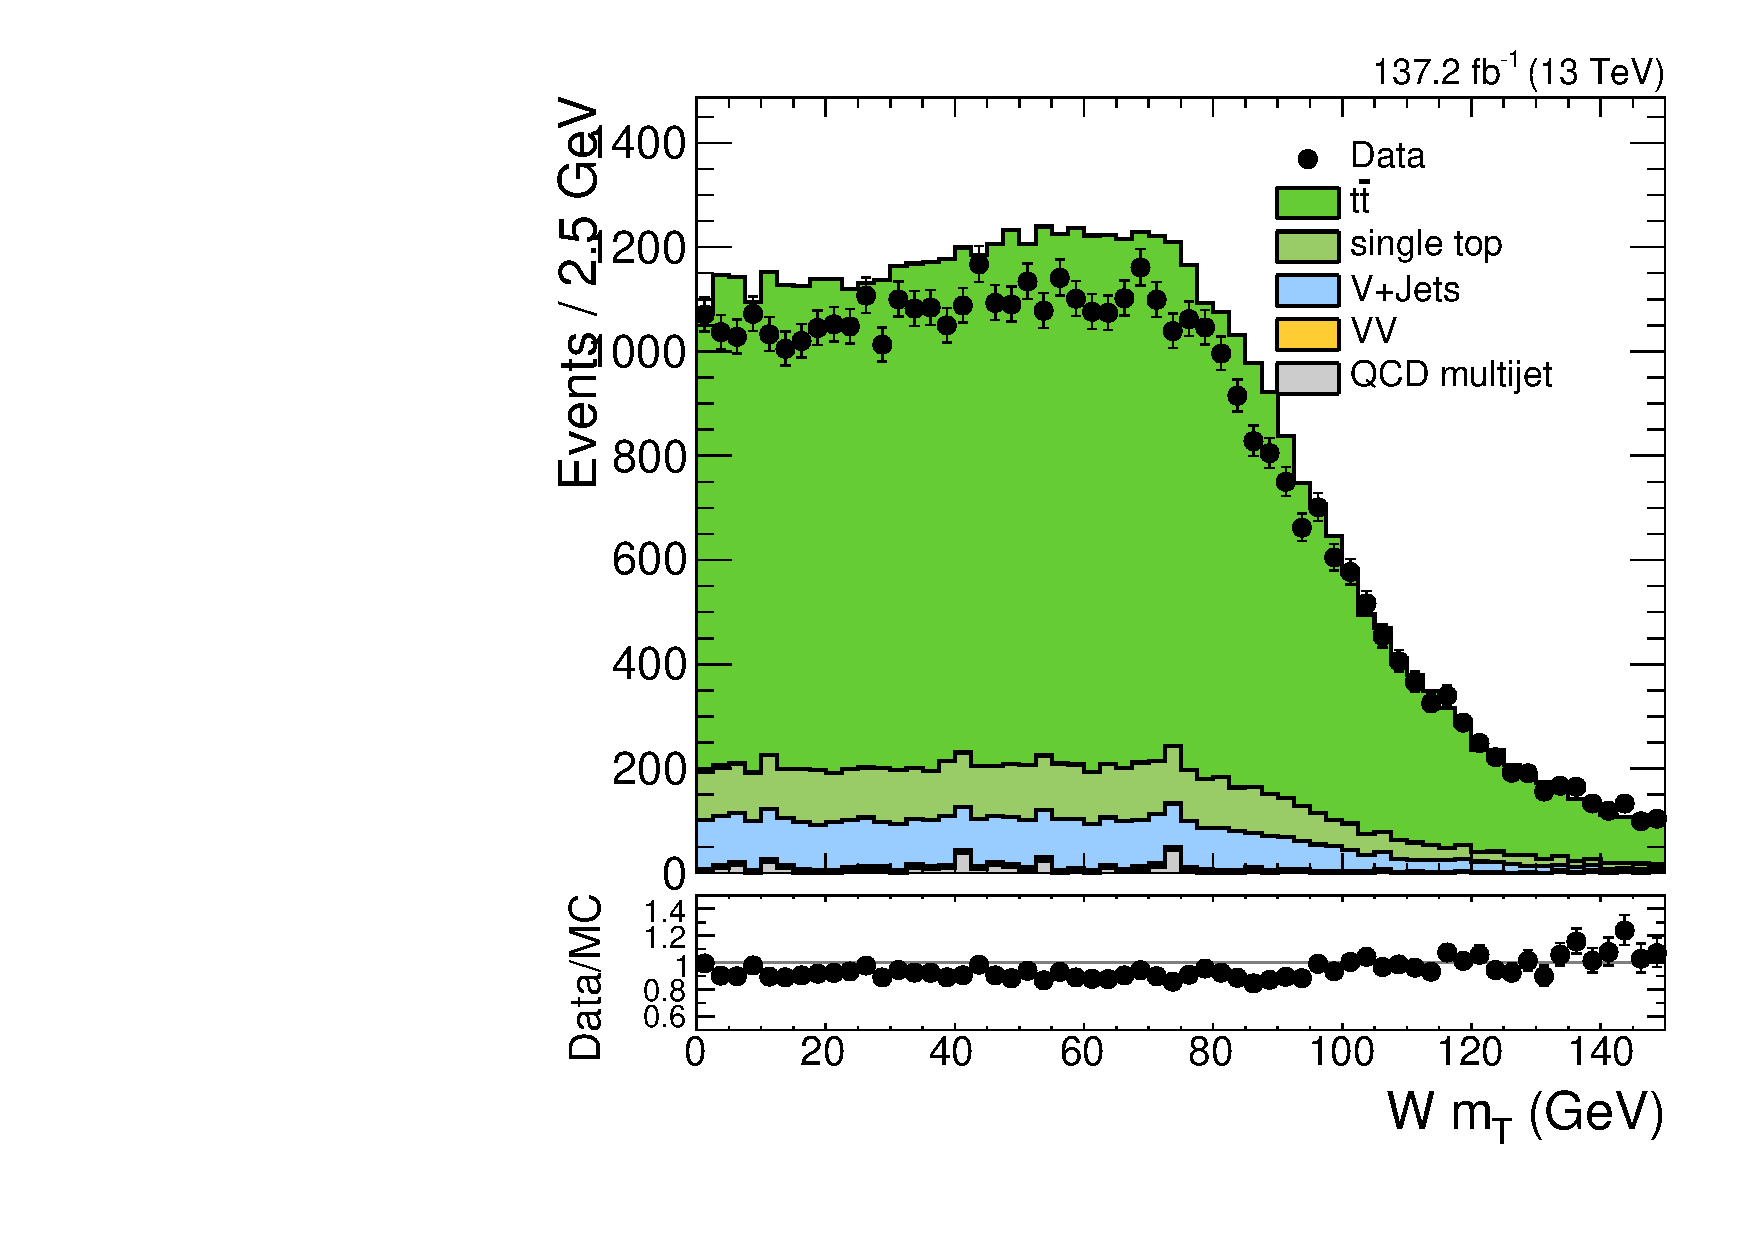
\includegraphics[width=0.4\textwidth]{fig/analysis/CR_b1_e_allP_allC_allE_Run2_lnujj_l1_mt.pdf}\\
  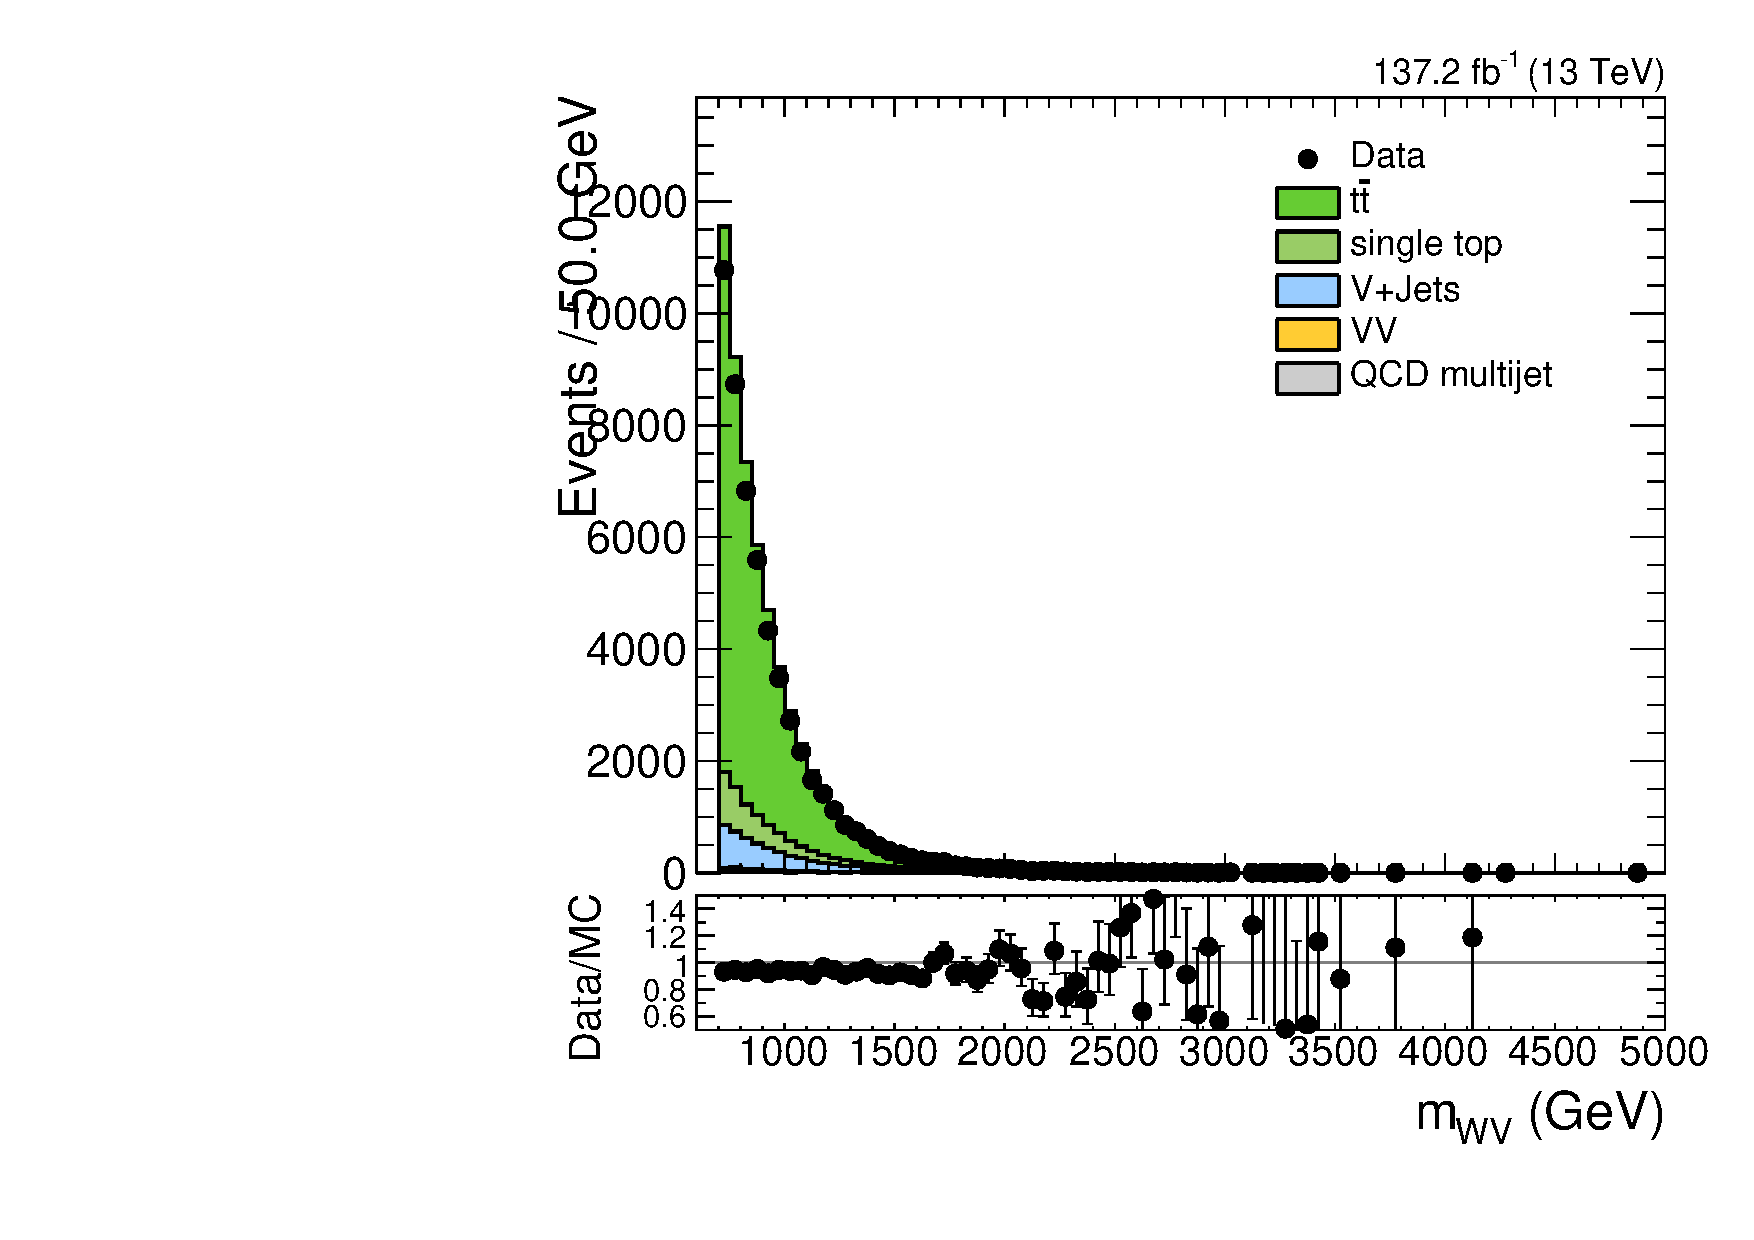
\includegraphics[width=0.4\textwidth]{fig/analysis/CR_b1_mu_allP_allC_allE_Run2_mWV.pdf}
  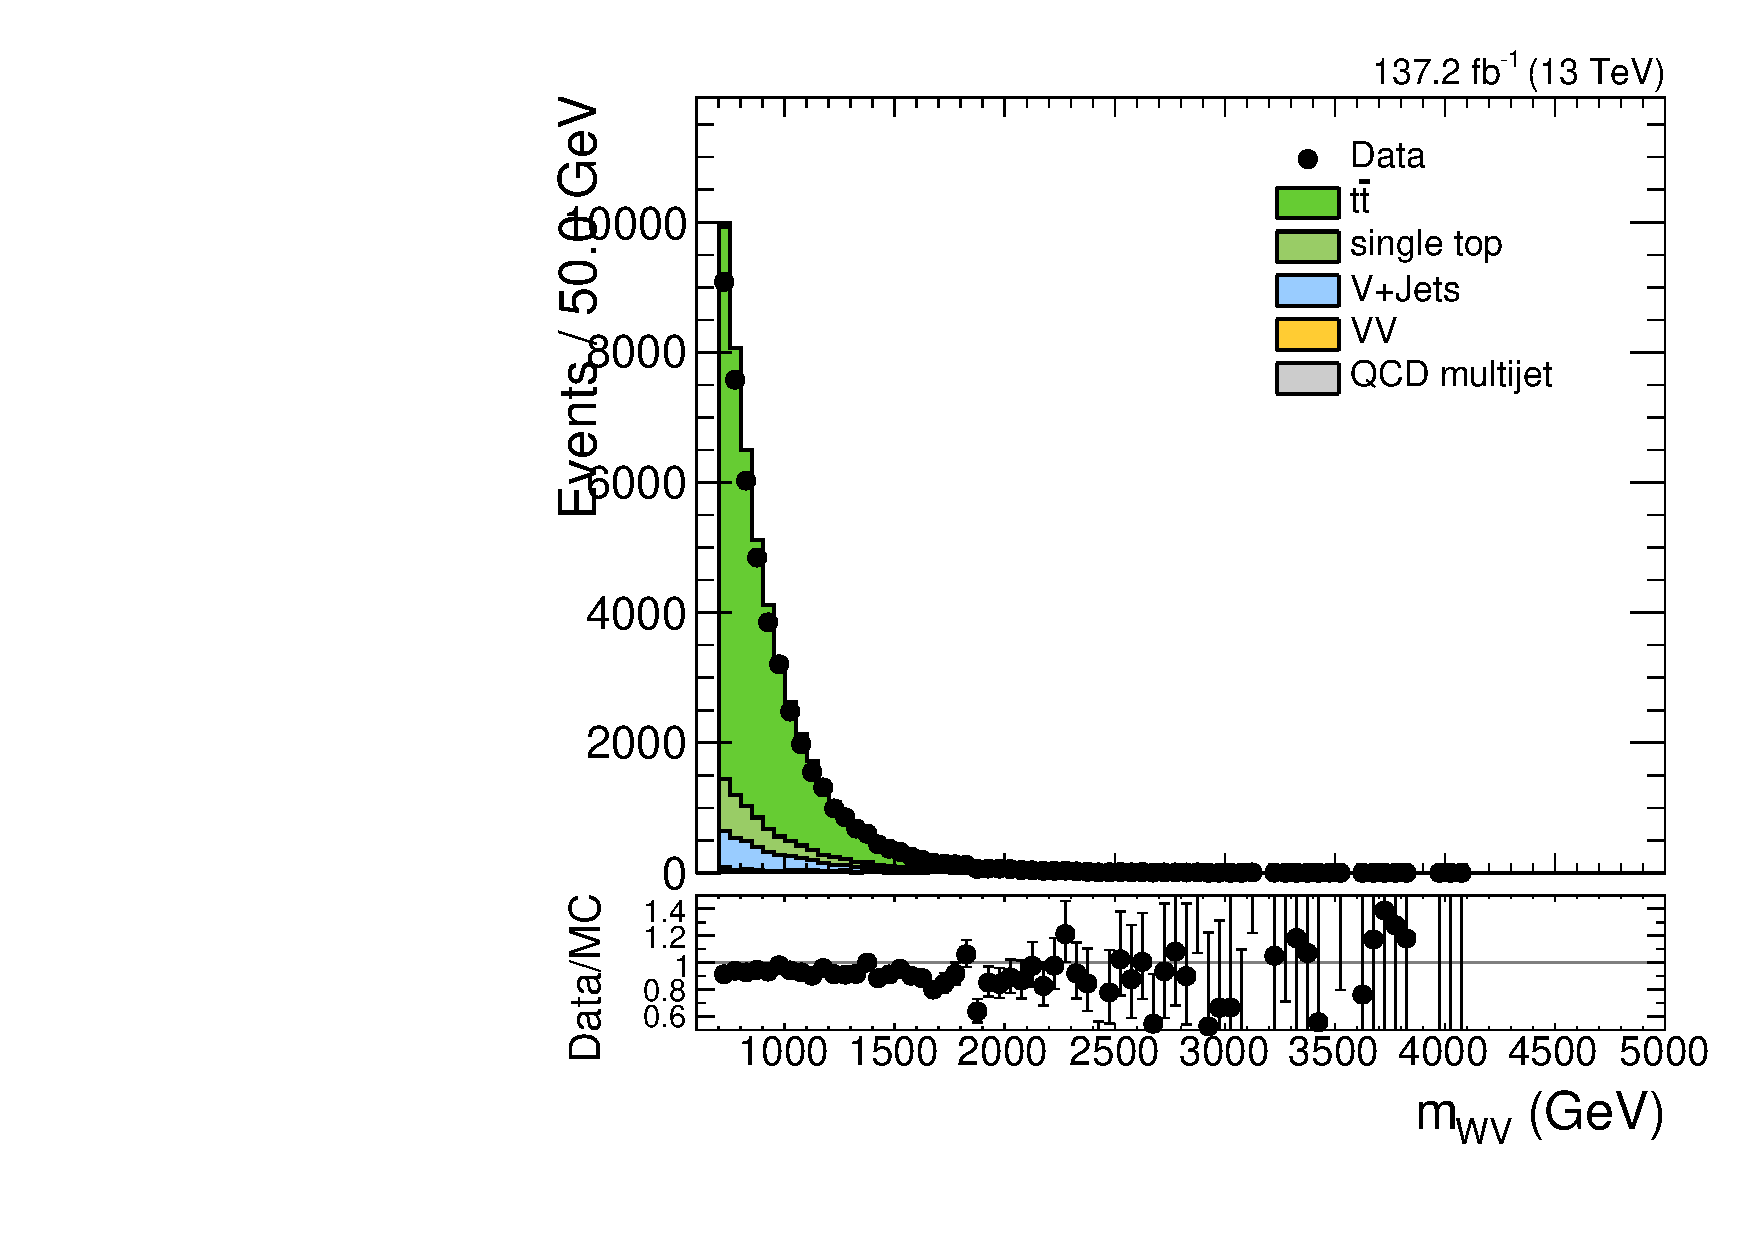
\includegraphics[width=0.4\textwidth]{fig/analysis/CR_b1_e_allP_allC_allE_Run2_mWV.pdf}\\
  \caption{
    Comparison plots between data and MC from Run 2 for different \Wlep-related observables, in the top-enriched control region.
    From top to bottom: \pt of the leptonic W, transverse mass of the leptonic W, diboson invariant mass.
    Left: muon channel, right: electron channel.
    }
  \label{fig:CR_controlPlotsRun2_2}
\end{figure}

\begin{figure}[htbp]
  \centering
  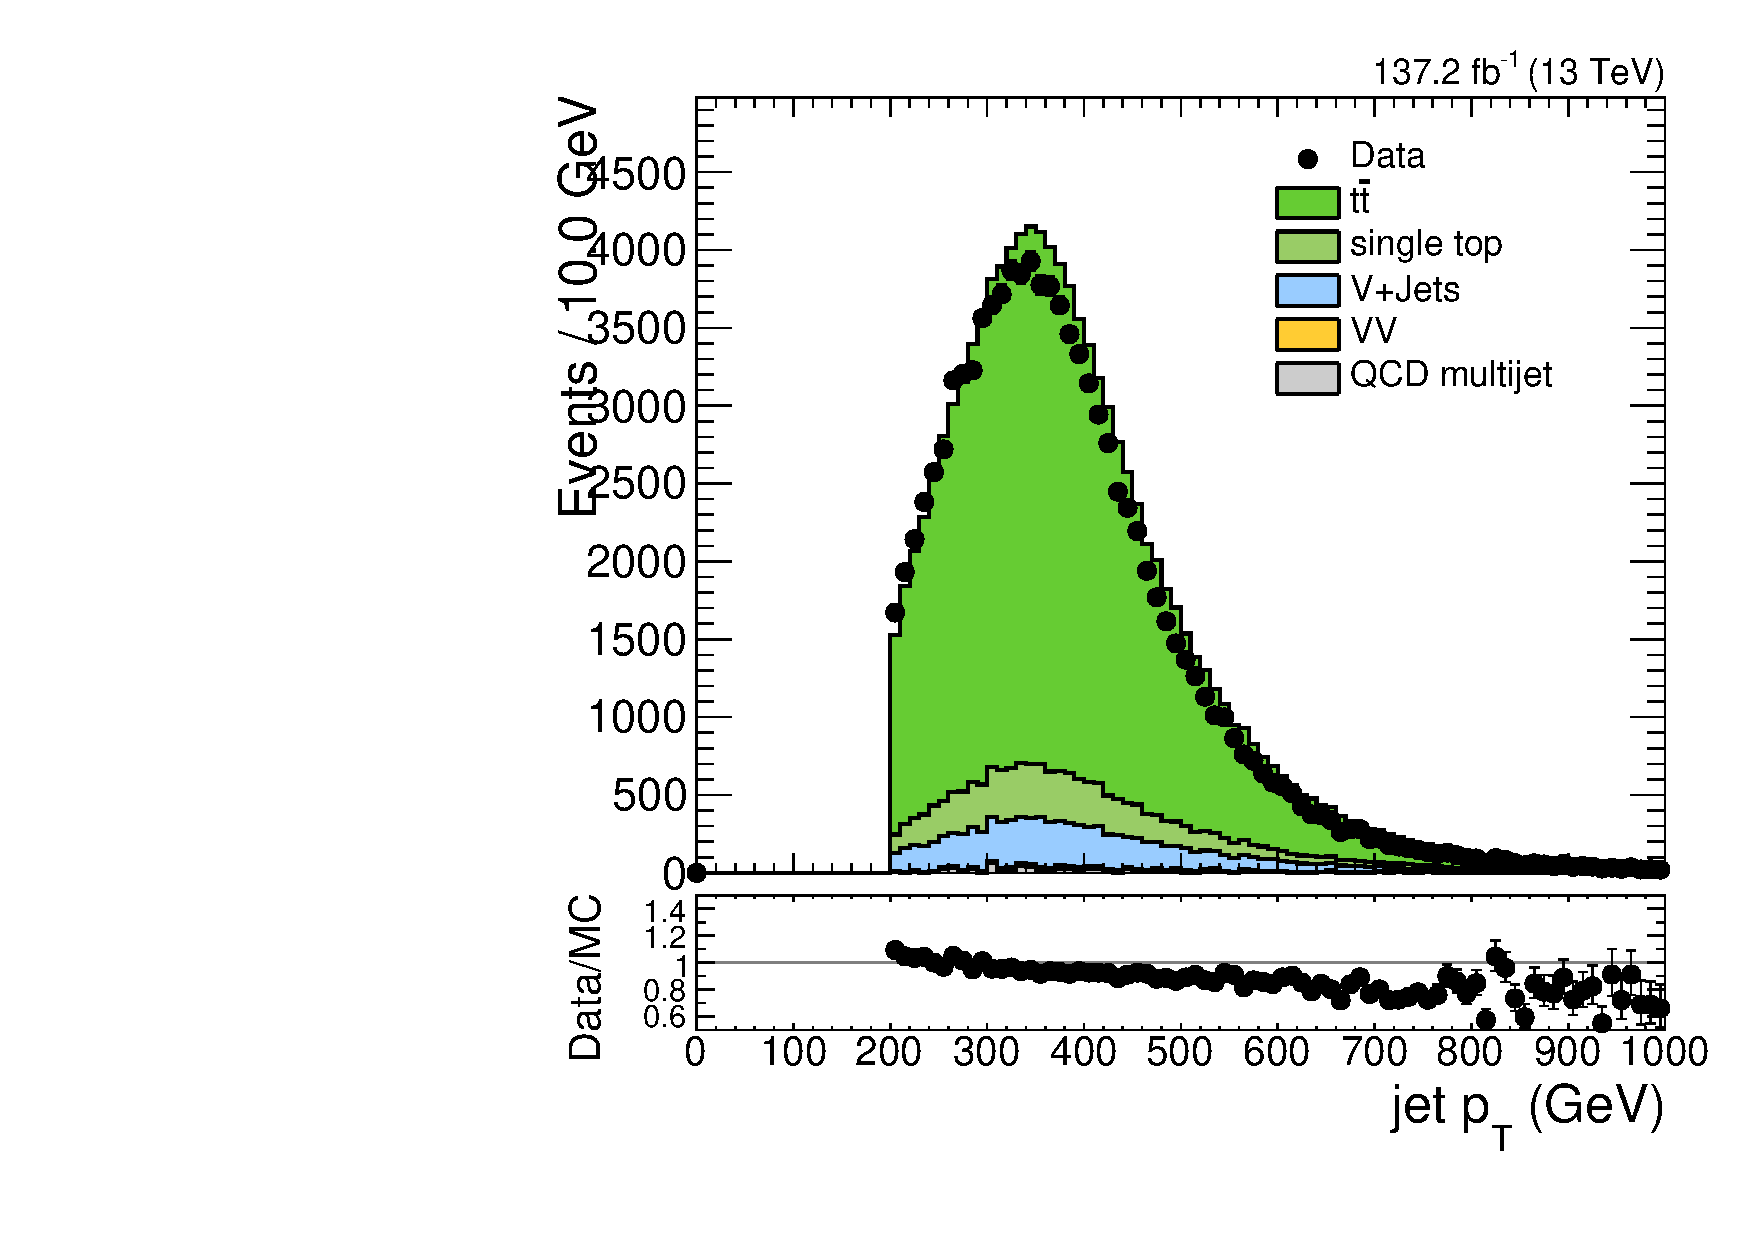
\includegraphics[width=0.4\textwidth]{fig/analysis/CR_b1_allL_allP_allC_allE_Run2_lnujj_l2_pt.pdf}
  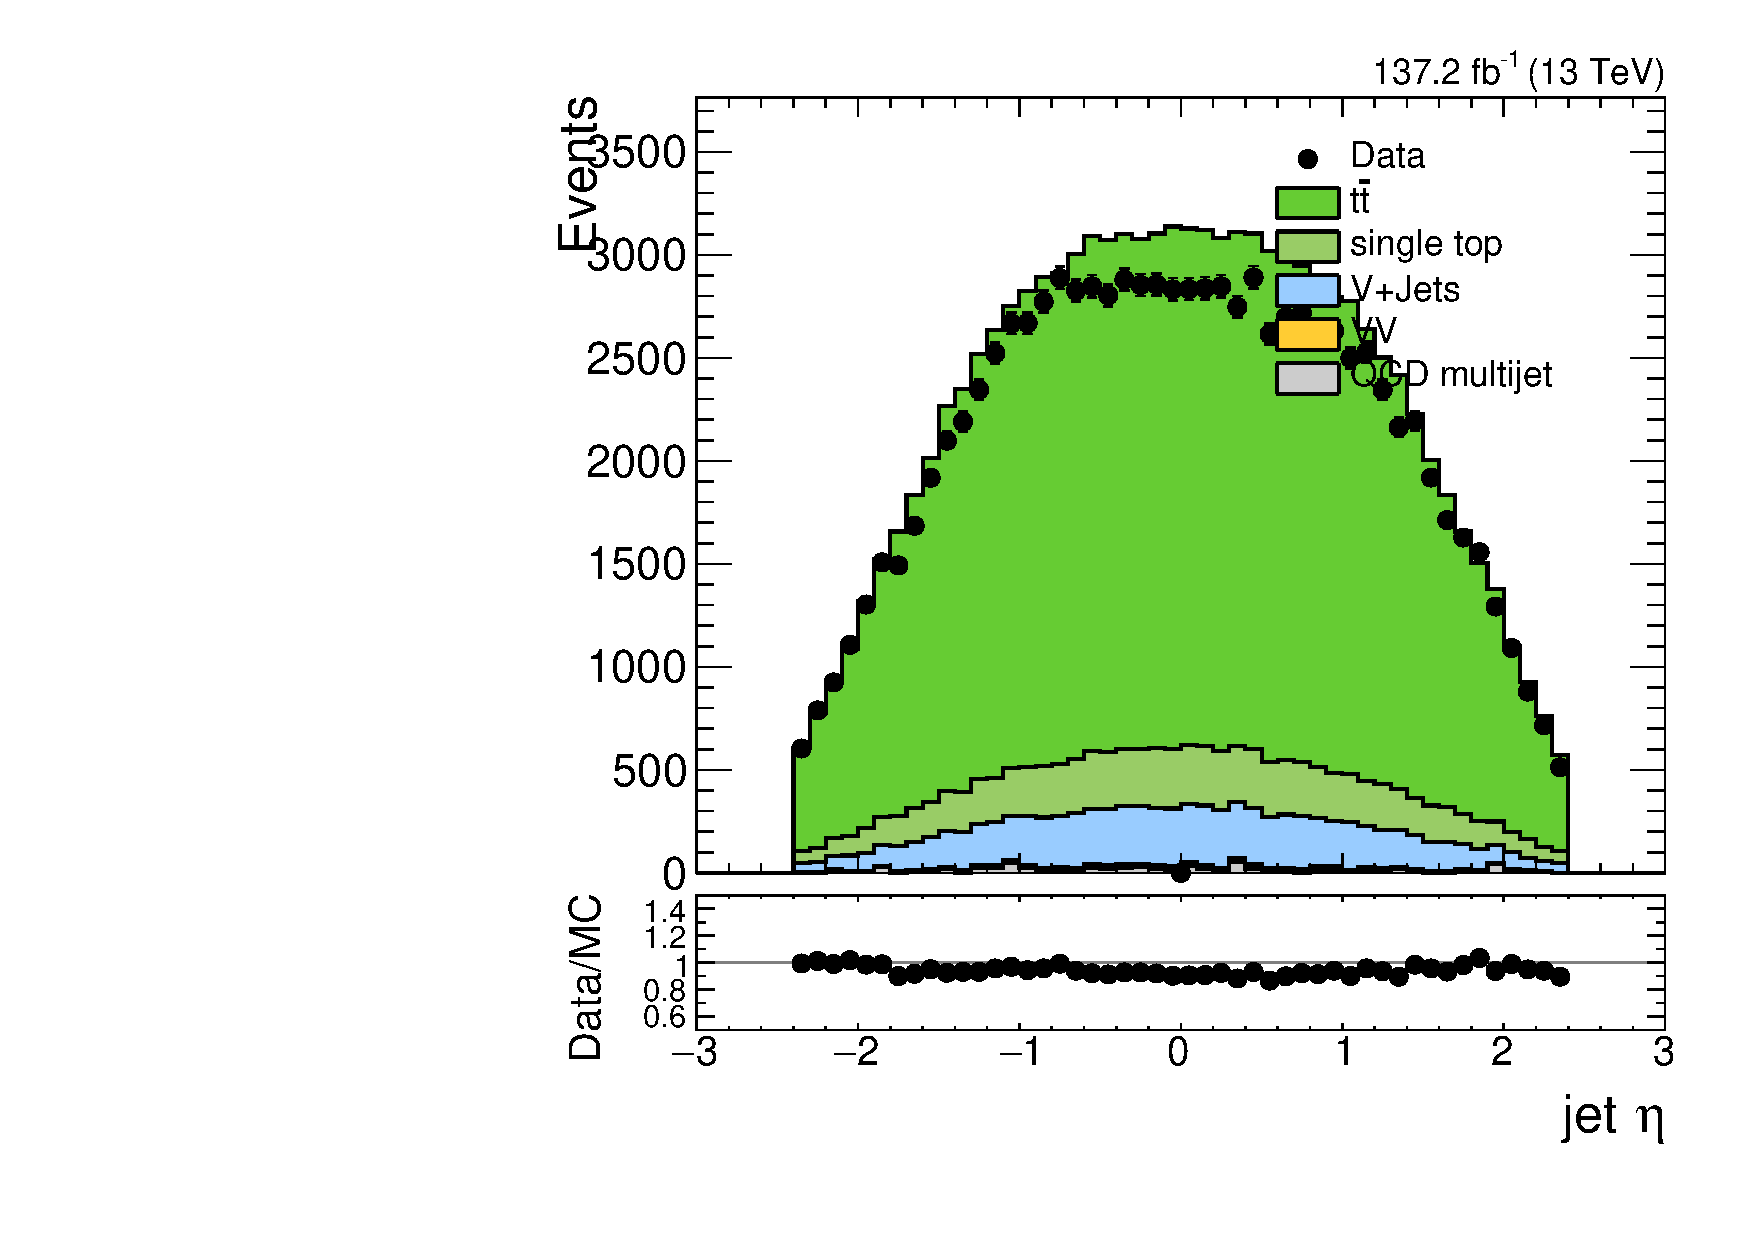
\includegraphics[width=0.4\textwidth]{fig/analysis/CR_b1_allL_allP_allC_allE_Run2_lnujj_l2_eta.pdf}\\
  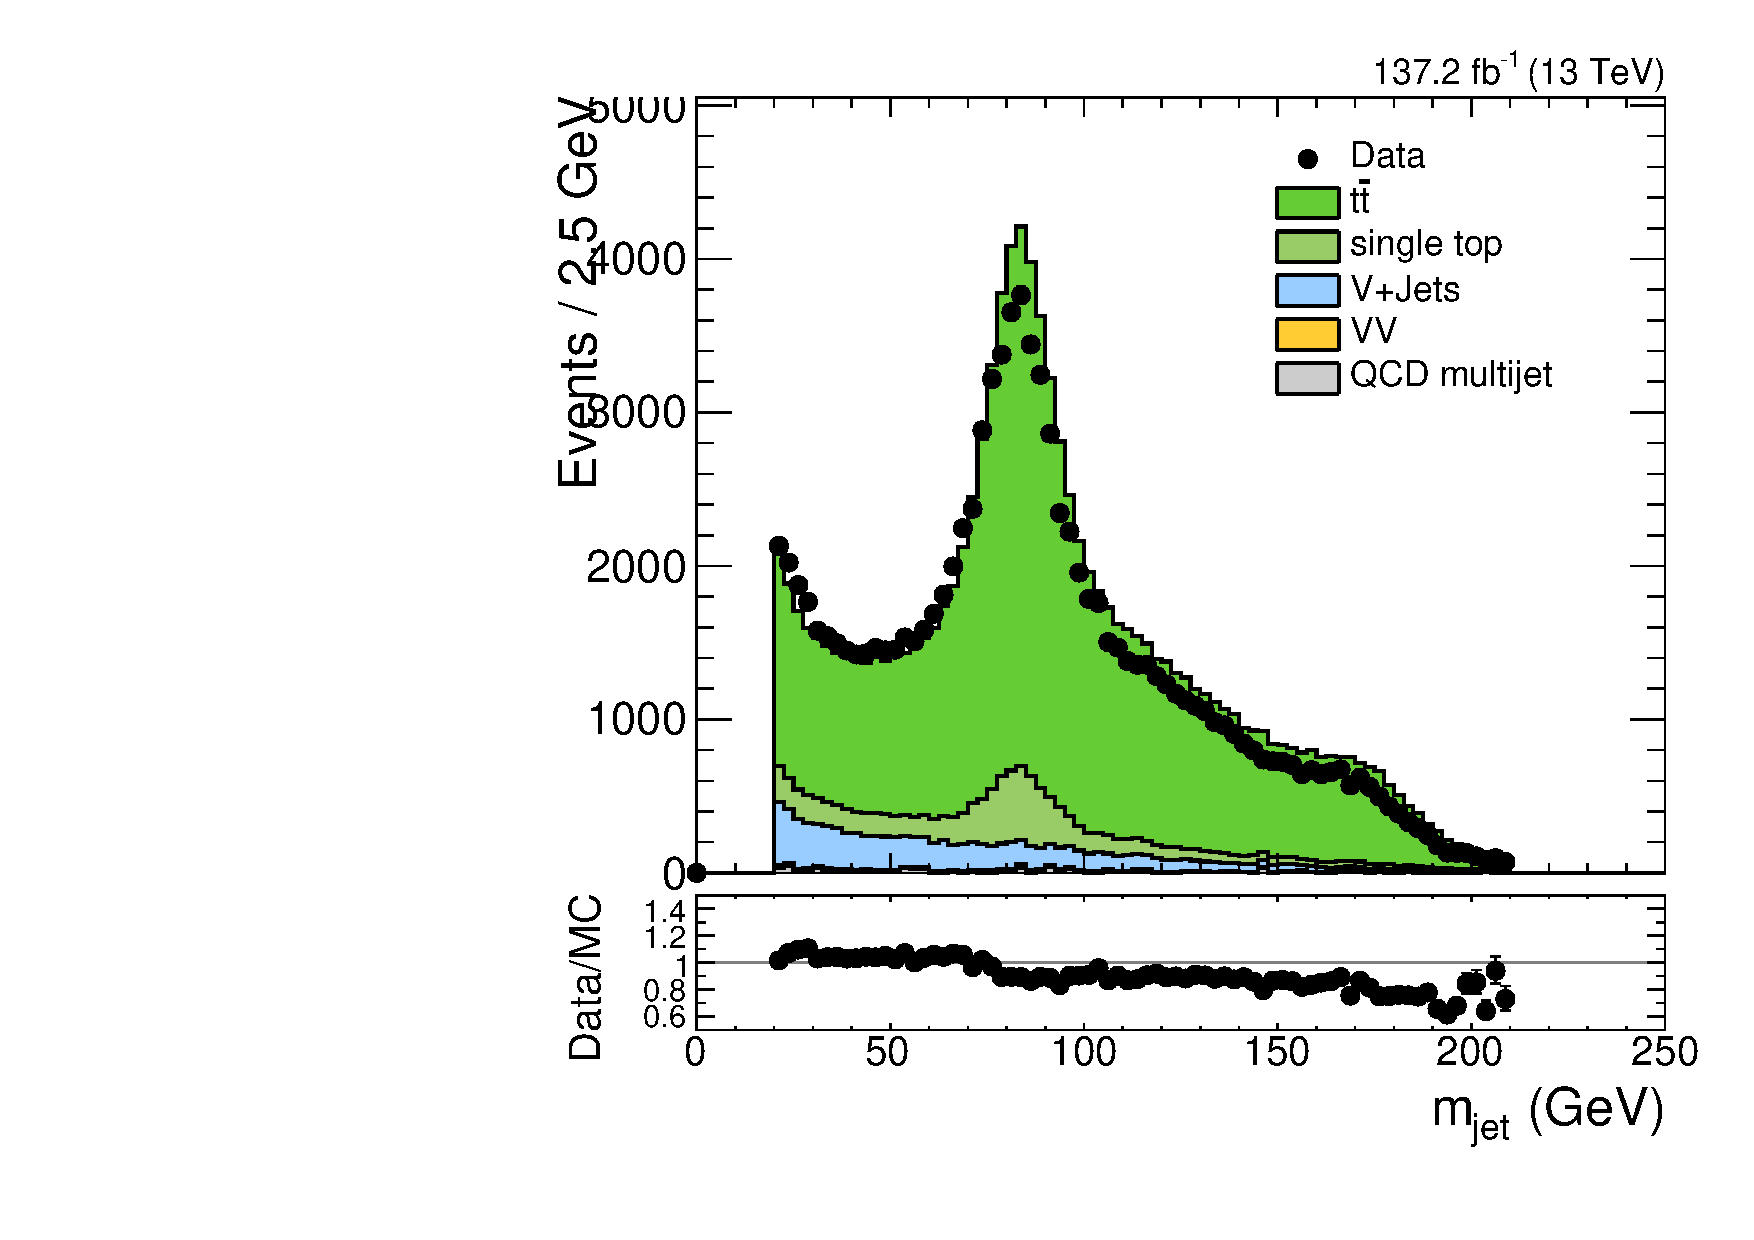
\includegraphics[width=0.4\textwidth]{fig/analysis/CR_b1_allL_allP_allC_allE_Run2_mjet.pdf}\\
  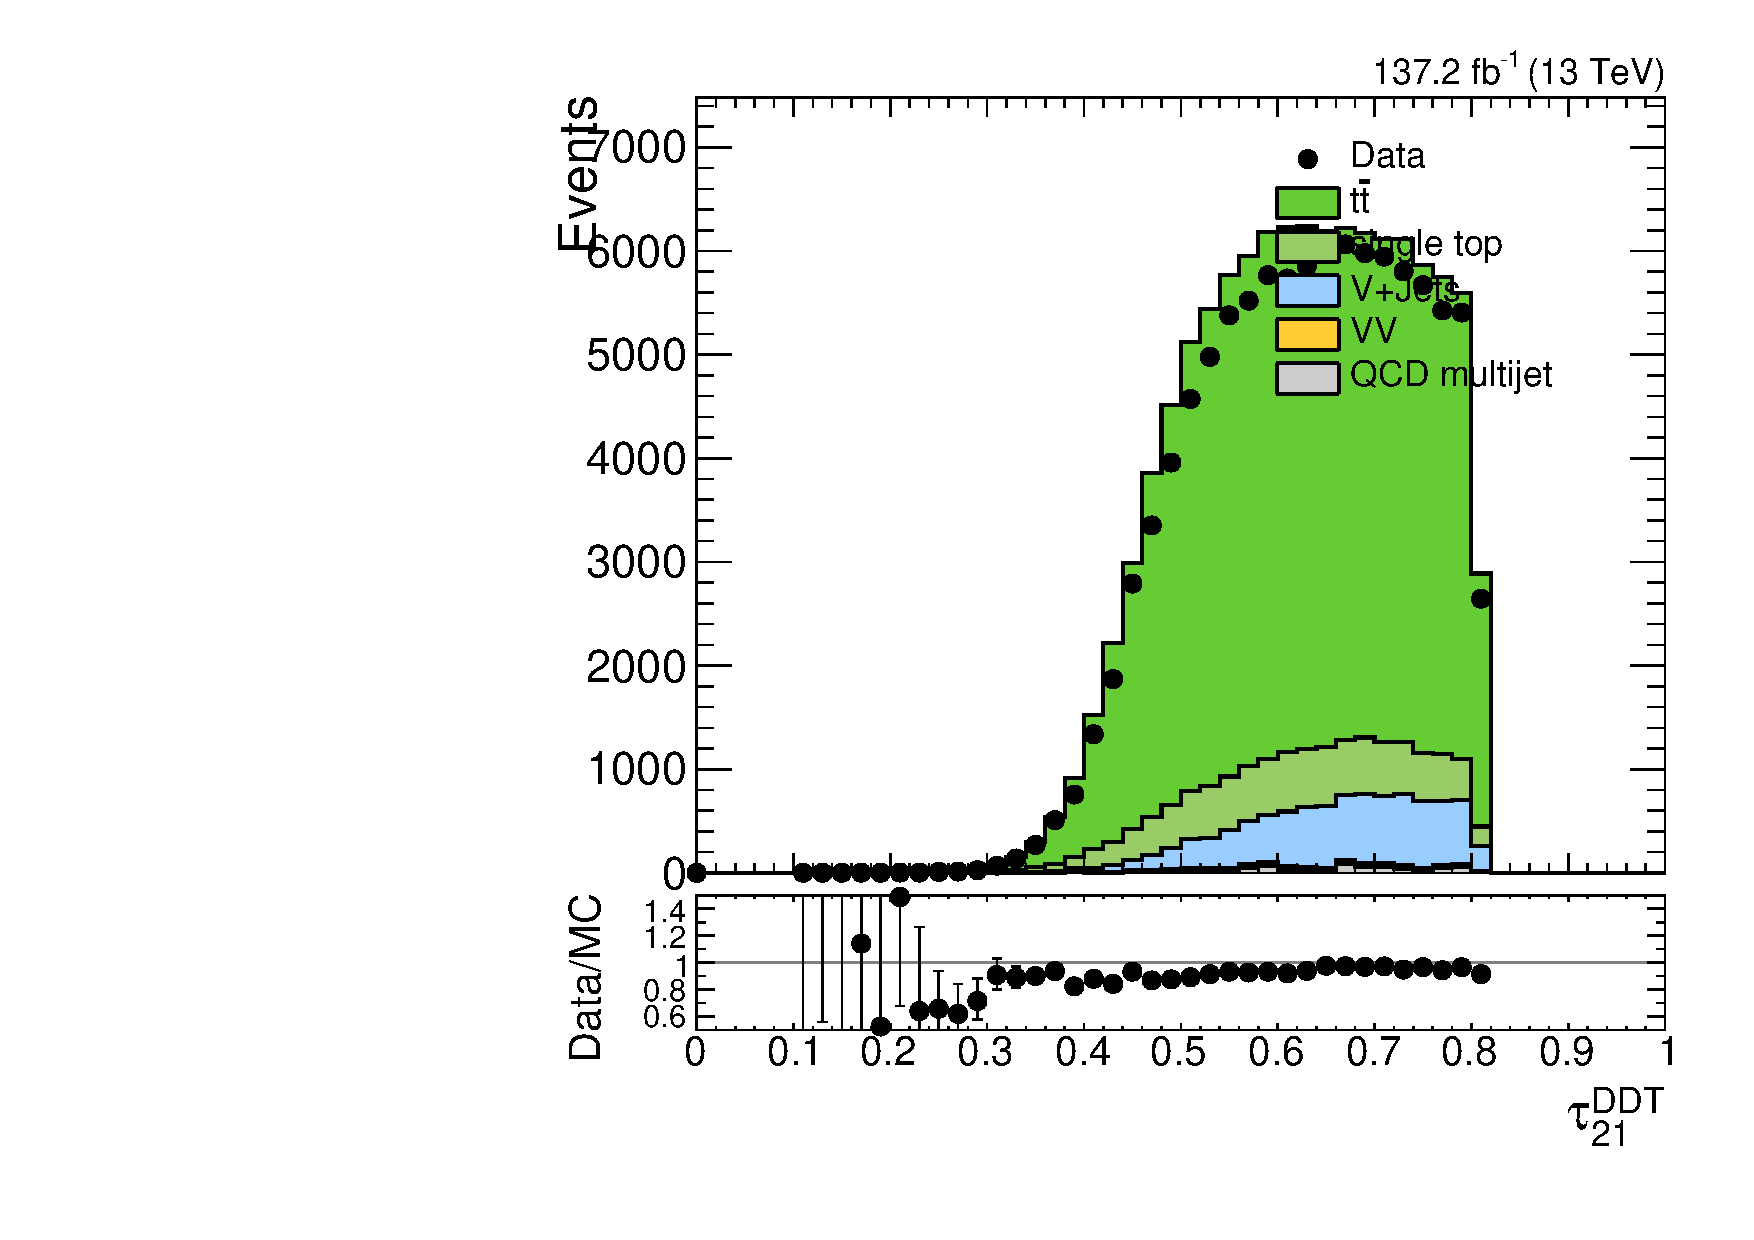
\includegraphics[width=0.4\textwidth]{fig/analysis/CR_b1_allL_allP_allC_allE_Run2_tau21DDT.pdf}
  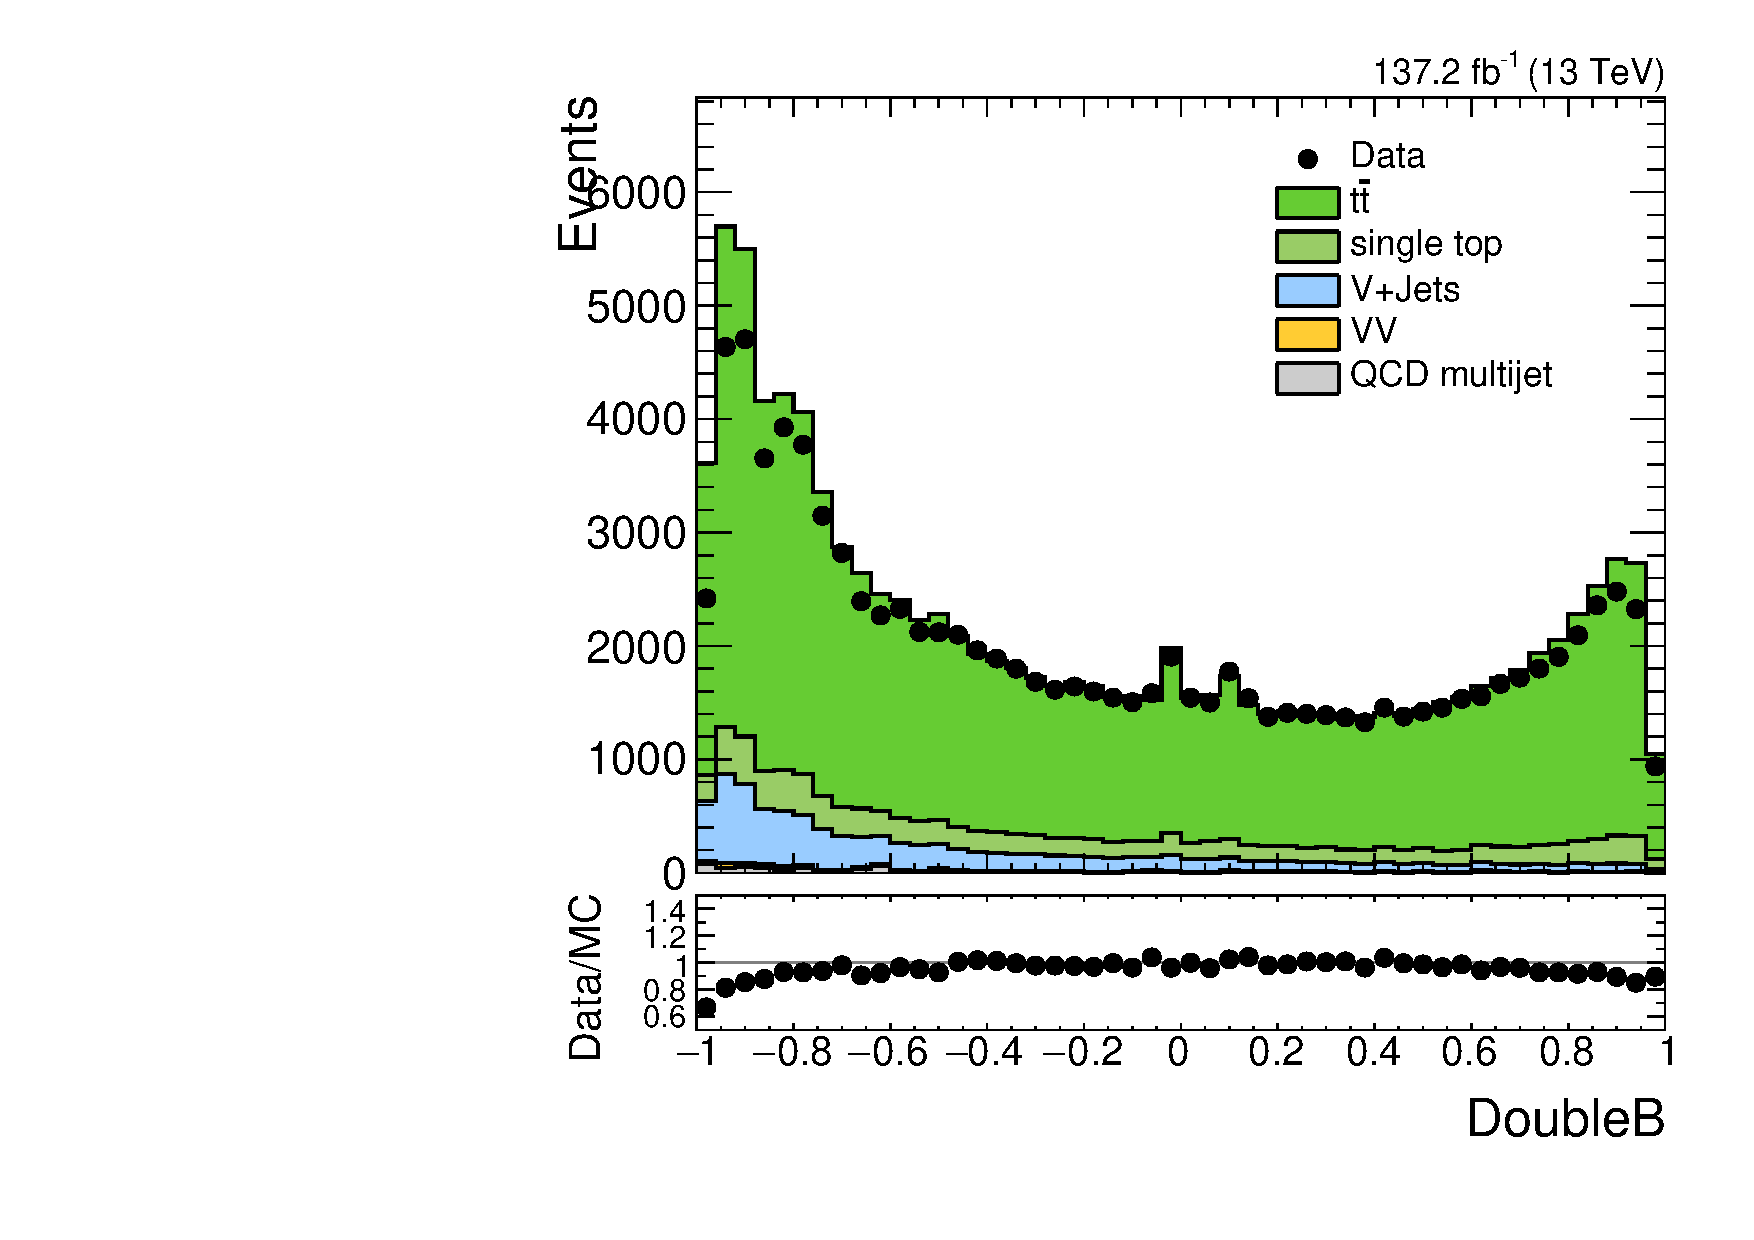
\includegraphics[width=0.4\textwidth]{fig/analysis/CR_b1_allL_allP_allC_allE_Run2_DoubleB.pdf}\\
  \caption{
    Comparison plots between data and MC from Run 2 for the \pt, $\eta$, \MJ (soft drop mass), \nsubjDDT, and \DoubleB tagger of the selected \Vhad candidate (leading AK8 jet), in the top-enriched control region.
  }
  \label{fig:CR_controlPlotsRun2_3}
\end{figure}

\begin{figure}[htbp]
  \centering
  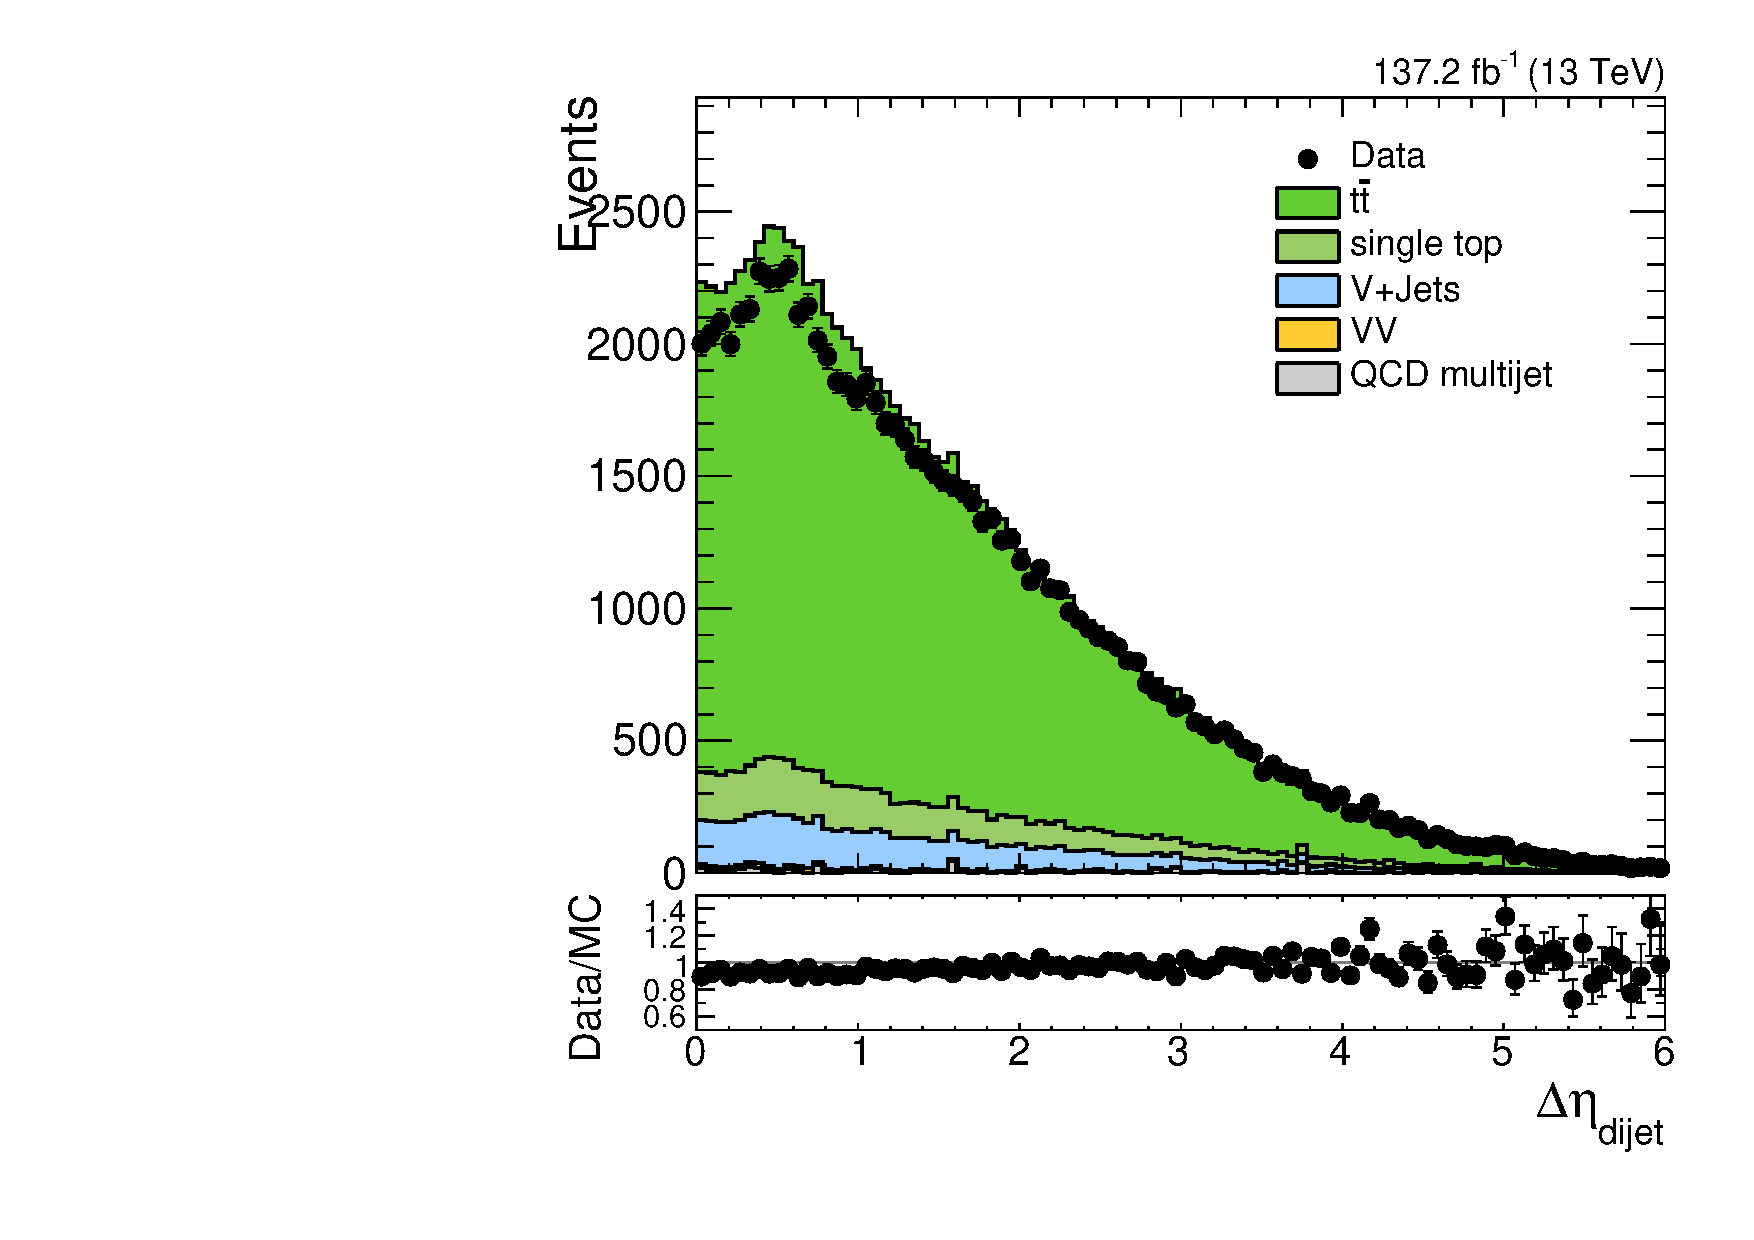
\includegraphics[width=0.4\textwidth]{fig/analysis/CR_b1_allL_allP_allC_allE_Run2_lnujj_vbfDEta.pdf}
  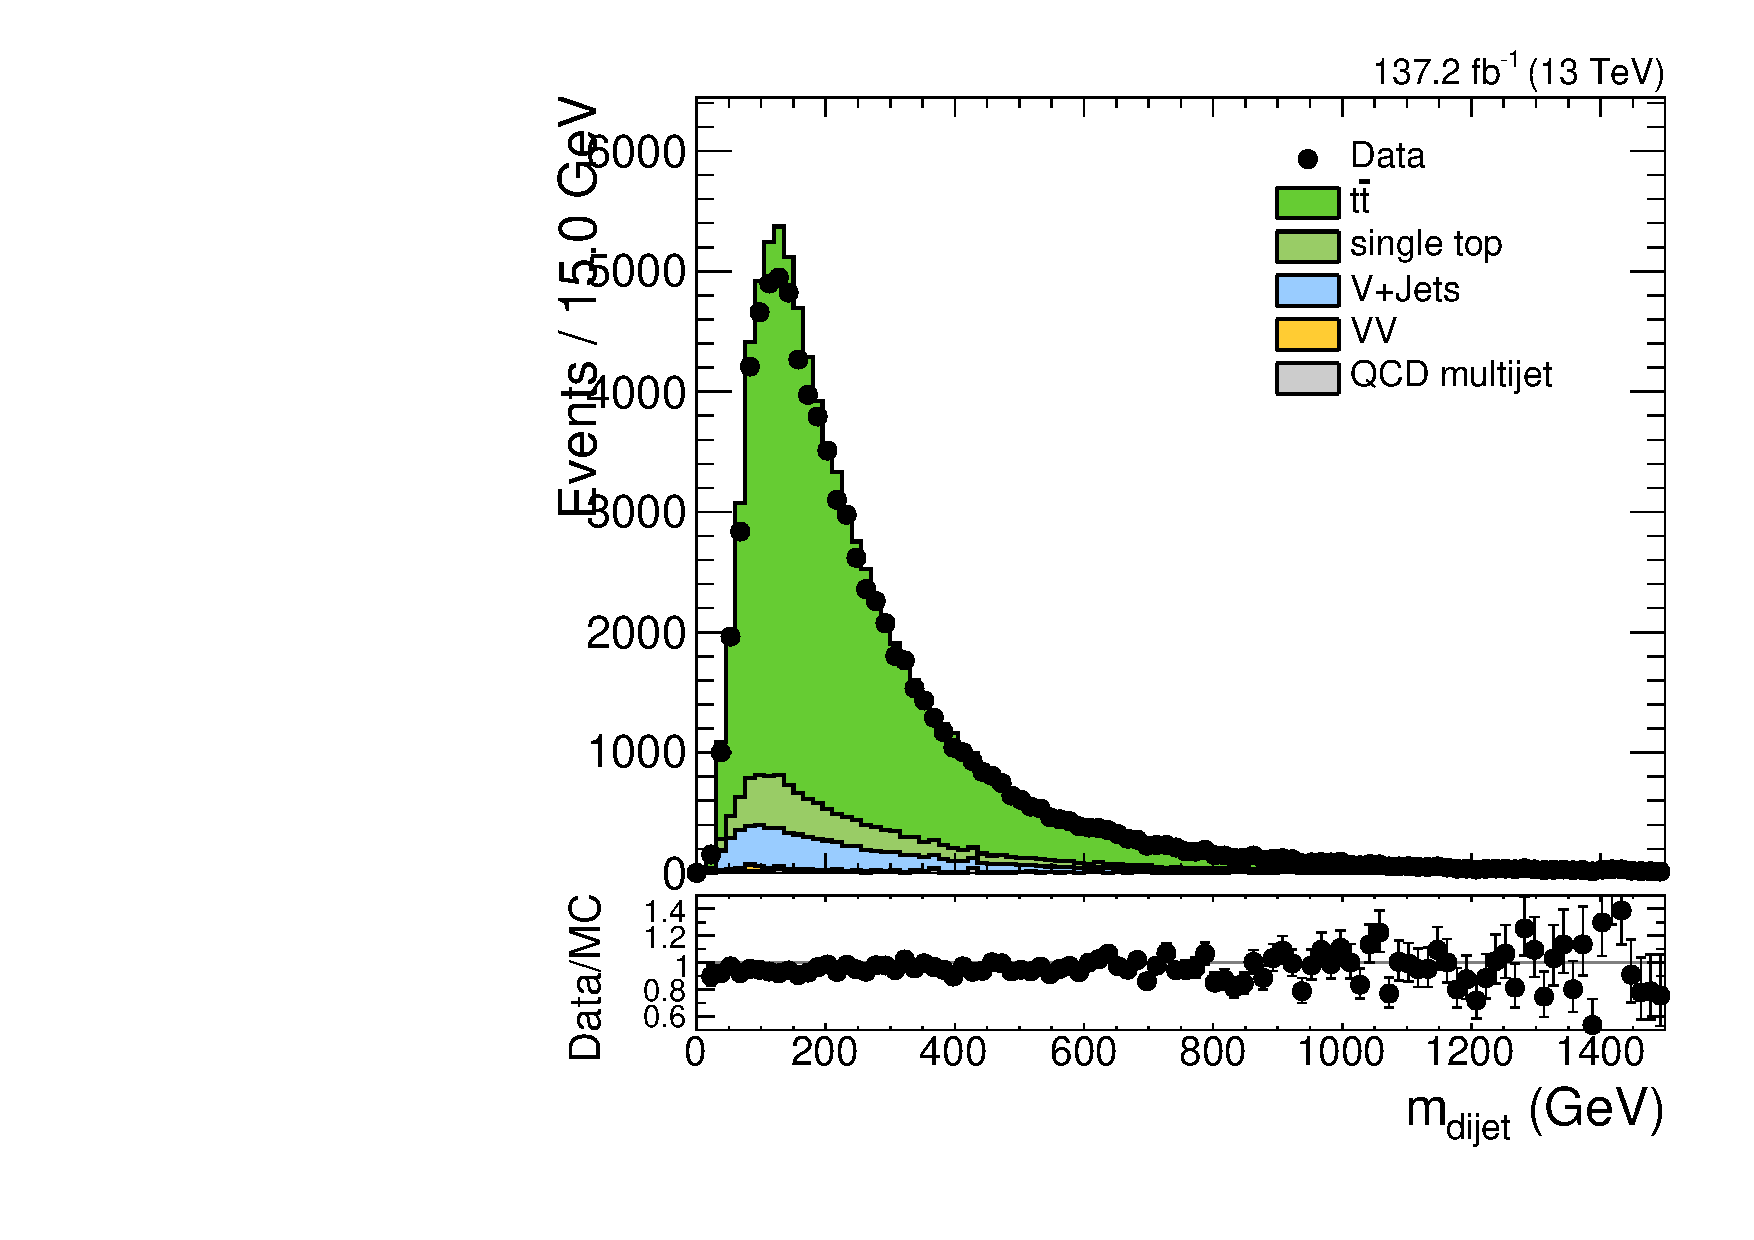
\includegraphics[width=0.4\textwidth]{fig/analysis/CR_b1_allL_allP_allC_allE_Run2_lnujj_vbfMass.pdf}\\
  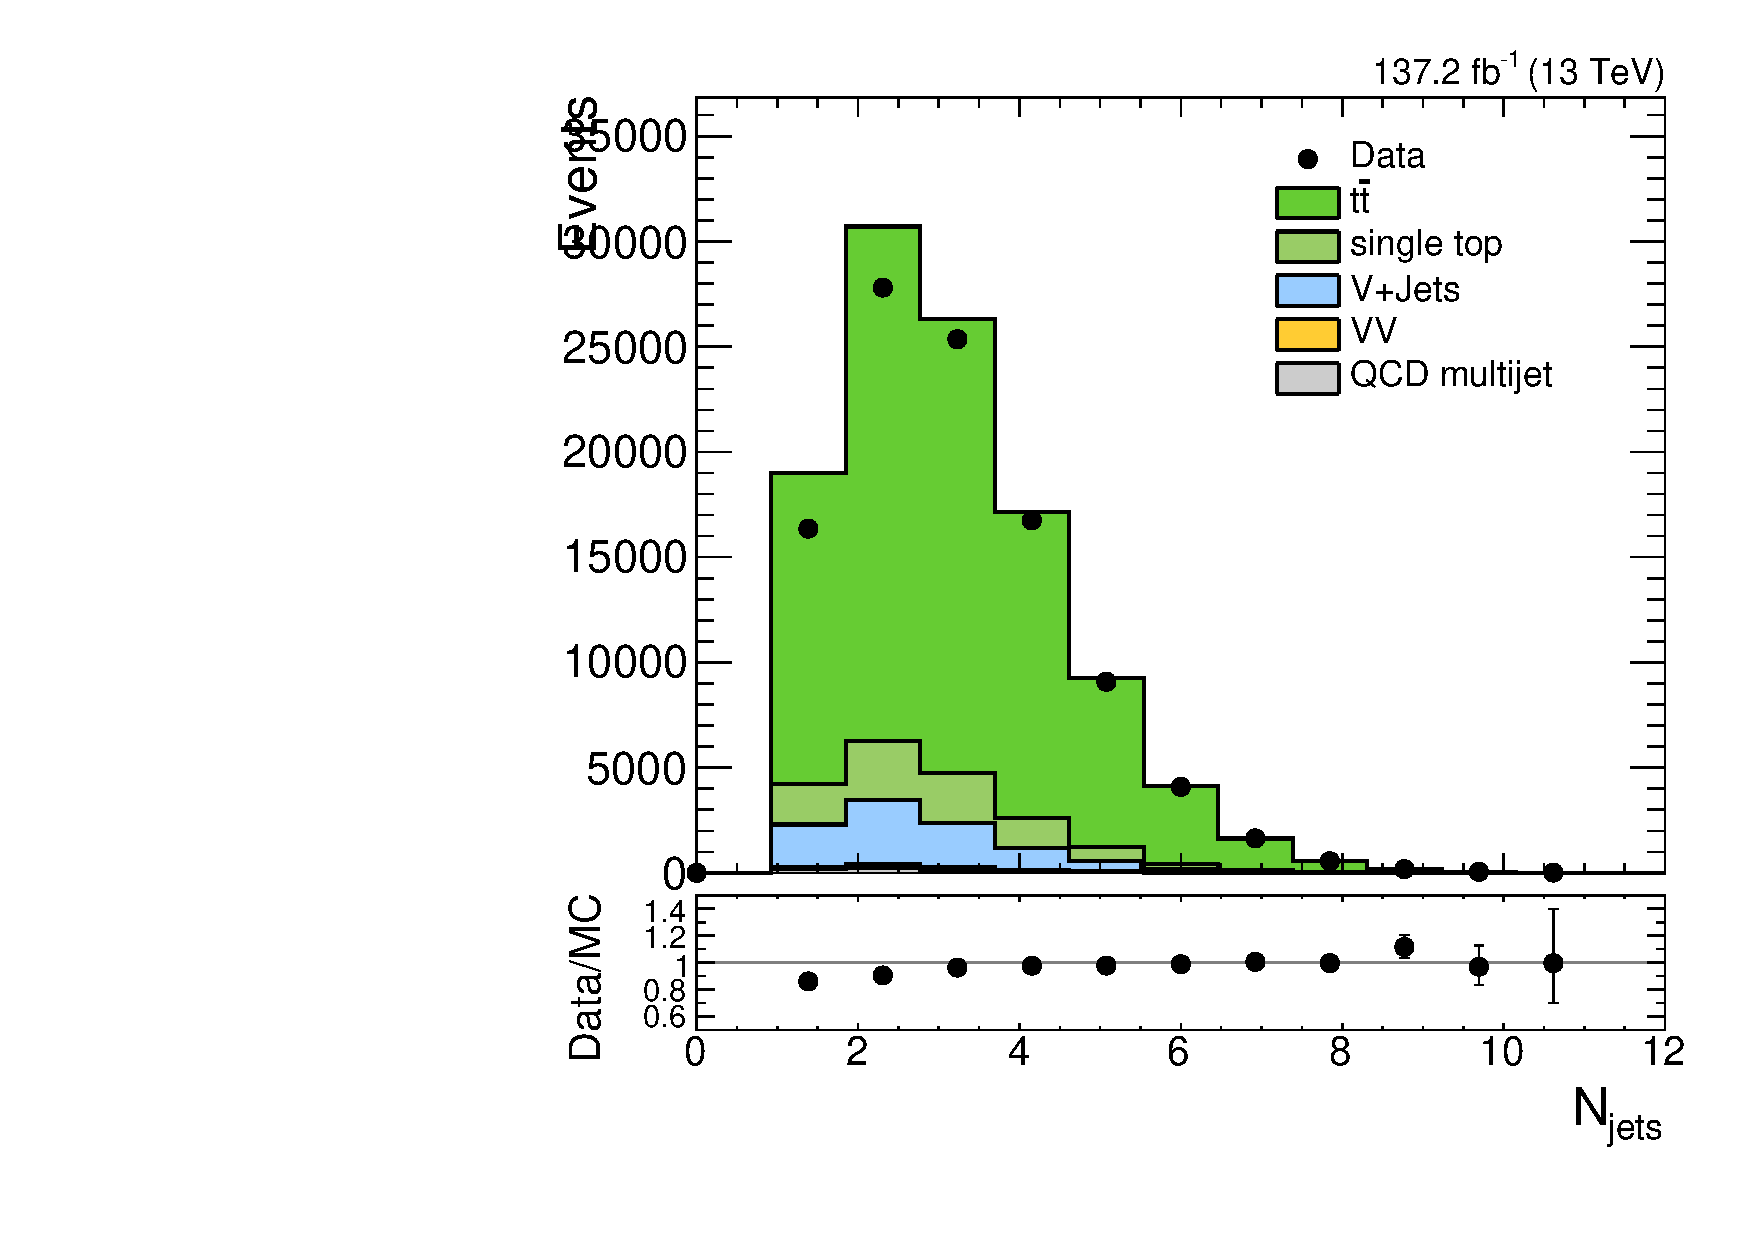
\includegraphics[width=0.4\textwidth]{fig/analysis/CR_b1_allL_allP_allC_allE_Run2_lnujj_nJets.pdf}
  \includegraphics[width=0.4\textwidth]{fig/analysis/CR_b1_allL_allP_allC_allE_Run2_dy.pdf}\\
  \caption{
    Comparison plots between data and MC from Run 2 for the separation in $\eta$ of the \VBF forward jets, invariant mass of the \VBF jets, number of selected standard jets, and rapidity separation between the reconstructed bosons, in the top-enriched control region.
  }
  \label{fig:CR_controlPlotsRun2_4}
\end{figure}

\subsection{Electron Negative Endcap Issue}

% Endcap issue
During Run 319077, the two HCAL towers HEM15 and HEM16 were non-operational, and the data obtained from the electron channel for the \Wtolnu candidate in those regions results in an excess of events that can be seen in figure~\ref{fig:SB_controlPlots2018_electronexcess}. % Citation
To remedy this, we exclude events recorded after Run 319077 if the lepton candidate is an electron and falls within the region $-1.55<\phi<-0.9$ and $-2.5<\eta<-1.479$.
Removing these events results in the correct behavior of the relevant kinematic variables for the electron candidate, and only discards 0.8\% of events in the signal region.

\begin{figure}[htbp]
  \centering
  \includegraphics[width=0.30\textwidth]{fig/analysis/SB_e_2018_lnujj_l1_l_eta.pdf}
  \includegraphics[width=0.30\textwidth]{fig/analysis/SB_e_2018_lnujj_l1_l_phi.pdf}
  \includegraphics[width=0.30\textwidth]{fig/analysis/SB_e_2018_met_phi.pdf}
  \caption{
    Comparison plots between 2018 data (including the HEM15 and HEM16 after Run 319077) and 2017 MC for the electron $\eta$, electron $\phi$, and $\phi$ of the missing transverse energy, in the jet mass sideband.
  }
  \label{fig:SB_controlPlots2018_electronexcess}
\end{figure}

\section{$V$-tagging Scale Factors}
\label{sec:vTag}

% Deriving scale factors
As mentioned previously, the top-enriched control region is obtained by inverting the $b$-tag veto and requiring the presence of at least one $b$-tagged jet, and the region is used to calibrate the performance of the soft drop algorithm and jet substructure variables on merged bosons.
In particular, the scale factors for the $V$-tagging selection in the HP and LP categories are derived in this region using a dedicated fit of the soft drop jet mass spectrum.
We also include events with $\nsubjDDT>0.80$ as a separate category denoted by NP to avoid bias resulting from only selecting HP and LP events.
This allows us to accurately model the $W$ peak for all categories used in the analysis.

\subsection{Fit Model}

% Fit model
Our fit model relies on two classes of events in the top-enriched region.
The first corresponds to resonant $W$ events that are the result of a top decay, with the $b$ jet outside of the AK8 jet.
The second class consists of non-resonant events resulting from random combinations of a merged AK8 jet.
To account for both of these types of events, we employ a fit model that uses a double crystal ball (DCB) for the $W$, another DCB for the partially reconstructed top quark, an exponential, and a uniform distribution.
Once the fit is performed, we then merge the second DCB, exponential, and uniform distributions to form a single non-resonant shape.

% Normalization
The explicit form of the fit model $f$ in each category (HP, LP, NP) is given by
\begin{align}
  & f(\mathrm{HP})=rSF^\mathrm{HP}N_W^\mathrm{HP}f_W^\mathrm{HP}+N_{NR}^\mathrm{HP}f_{NR}^\mathrm{HP},\label{eq:VtagFit1}\\
  & f(\mathrm{LP})=rSF^\mathrm{LP}N_W^\mathrm{LP}f_W^\mathrm{LP}+N_{NR}^\mathrm{LP}f_{NR}^\mathrm{LP},\label{eq:VtagFit2}\\
  & f(\mathrm{NP})=r\bqty{N_\mathrm{Total}-SF^\mathrm{HP}N_W^\mathrm{HP}-SF^\mathrm{LP}N_W^\mathrm{LP}}f_W^\mathrm{NP}+N_{NR}^\mathrm{NP}+f_{NR}^\mathrm{NP},\label{eq:VtagFit3}
\end{align}
where $f_W$ is the resonant distribution for the $W$ jet, $f_{NR}$ is the non-resonant shape, $r$ is a global scale factor accounting for lepton efficiency and luminosity, $N_{W}^\mathrm{HP}$, $N_{W}^\mathrm{LP}$, $N_{W}^\mathrm{NP}$, and $N_\mathrm{Total}$ are the number of expected events in simulation for all three categories and the total number of events, and the $SF$ are scale factors for the HP and LP categories.
This normalization is chosen to account for migration between categories.

\subsection{Fit Results}

% Fit results
We perform the fit of equations~\ref{eq:VtagFit1}-\ref{eq:VtagFit3} in a jet mass window of 20-$145\unit{GeV}$.
The resulting post-fit distributions for all three years and the full Run 2 dataset and MC samples can be seen in figure~\ref{fig:VTag_postfit_Run2}.
Table~\ref{tab:VTagFactors} shows the $V$-tagging scale factors in the HP and LP categories obtained by the fit for all years and the full Run 2 dataset, and table~\ref{tab:VScaleRes} shows the scale factors for the jet mass scale and resolution again for all years and for the full Run 2 dataset.
For the analysis we use the Run 2 scale factors in the computation of the expected signal normalizations, and the Run 2 uncertainties are used as a flat systematic uncertainty for the signal normalizations.
The scale factors for the jet mass scale and resolution are used as corrections to the signal shapes and $W$ peak for the resonant background templates.

\begin{figure}[htbp]
  \centering
  \includegraphics[width=0.3\textwidth]{fig/analysis/PostFit__MJJ__allC_allL_HP_2016.pdf}
  \includegraphics[width=0.3\textwidth]{fig/analysis/PostFit__MJJ__allC_allL_LP_2016.pdf}
  \includegraphics[width=0.3\textwidth]{fig/analysis/PostFit__MJJ__allC_allL_NP_2016.pdf}\\
  \includegraphics[width=0.3\textwidth]{fig/analysis/PostFit__MJJ__allC_allL_HP_2017.pdf}
  \includegraphics[width=0.3\textwidth]{fig/analysis/PostFit__MJJ__allC_allL_LP_2017.pdf}
  \includegraphics[width=0.3\textwidth]{fig/analysis/PostFit__MJJ__allC_allL_NP_2017.pdf}\\
  \includegraphics[width=0.3\textwidth]{fig/analysis/PostFit__MJJ__allC_allL_HP_2018.pdf}
  \includegraphics[width=0.3\textwidth]{fig/analysis/PostFit__MJJ__allC_allL_LP_2018.pdf}
  \includegraphics[width=0.3\textwidth]{fig/analysis/PostFit__MJJ__allC_allL_NP_2018.pdf}\\
  \includegraphics[width=0.3\textwidth]{fig/analysis/PostFit__MJJ__allC_allL_HP_Run2.pdf}
  \includegraphics[width=0.3\textwidth]{fig/analysis/PostFit__MJJ__allC_allL_LP_Run2.pdf}
  \includegraphics[width=0.3\textwidth]{fig/analysis/PostFit__MJJ__allC_allL_NP_Run2.pdf}\\
  \caption{
    Post-fit distributions for the background MC and data set for all three years and Run 2 (from top to bottom: 2016, 2017, 2018, Run 2), and for the three purity categories (from left to right: HP, LP, NP).
  }
  \label{fig:VTag_postfit_Run2}
\end{figure}

\begin{table}[htbp]
  \centering
  % !TEX root = ../../thesis.tex
\footnotesize
\begin{tabular}{|ccc|}
  \hline
  Year & HP & LP \\
  \hline
  2016  & $1.02 \pm 0.04$ (stat) $\pm 0.03$ (syst) & $0.98 \pm 0.02$ (stat) $\pm 0.03$ (syst)  \\
  2017  & $0.83 \pm 0.04$ (stat) $\pm 0.03$ (syst) & $1.10 \pm 0.02$ (stat) $\pm 0.03$ (syst)  \\
  2018  & $0.87 \pm 0.03$ (stat) $\pm 0.03$ (syst) & $1.08 \pm 0.02$ (stat) $\pm 0.03$ (syst)  \\
  Run 2 & $0.88 \pm 0.02$ (stat) $\pm 0.03$ (syst) & $1.06 \pm 0.02$ (stat) $\pm 0.03$ (syst)  \\
  \hline
\end{tabular}

  \caption{
    $V$-tagging scale factors for the HP and LP categories obtained from the fit process.
  }
  \label{tab:VTagFactors}
\end{table}

\begin{table}[htbp]
  \centering
  % !TEX root = ../../thesis.tex
\footnotesize
\begin{tabular}{|ccc|}
  \hline
  Year & scale & resolution \\
  \hline
  2016  & $0.991 \pm 0.003$ (stat) $\pm 0.002$ (syst) & $1.00 \pm 0.03$ (stat) $\pm 0.02$ (syst) \\
  2017  & $0.989 \pm 0.003$ (stat) $\pm 0.002$ (syst) & $1.07 \pm 0.04$ (stat) $\pm 0.02$ (syst) \\
  2018  & $0.987 \pm 0.002$ (stat) $\pm 0.002$ (syst) & $1.08 \pm 0.03$ (stat) $\pm 0.02$ (syst) \\
  Run 2 & $0.990 \pm 0.002$ (stat) $\pm 0.002$ (syst) & $1.08 \pm 0.02$ (stat) $\pm 0.02$ (syst) \\
  \hline
\end{tabular}

  \caption{
    Scale factors for the jet mass scale and resolution obtained from the fit process.
  }
  \label{tab:VScaleRes}
\end{table}

\subsection{Momentum Dependence}

% Momentum dependence
We also conduct a study on the dependence of the $V$-tagging scale factors as a function of the diboson invariant mass \MVV to apply a systematic uncertainty on the $V$-tagging process.
To do so, we measure the $V$-tagging scale factors for the full Run 2 dataset, but in three different binnings of \MVV.
We apply a low-mass binning of $[0.6,0.8\unit{TeV}]$, a mid-mass binning of $[0.8,1.0\unit{TeV}]$, and a high-mass binning of $[1.0,1.5\unit{TeV}]$.
The resulting post-fit distributions for all three binnings and for all purity categories may be see in figure~\ref{fig:VTag_postfit_massdep}.

\begin{figure}[htbp]
  \centering
  \includegraphics[width=0.3\textwidth]{fig/analysis/PostFit__MJJ__allC_allL_HP_Low.pdf}
  \includegraphics[width=0.3\textwidth]{fig/analysis/PostFit__MJJ__allC_allL_LP_Low.pdf}
  \includegraphics[width=0.3\textwidth]{fig/analysis/PostFit__MJJ__allC_allL_NP_Low.pdf}\\
  \includegraphics[width=0.3\textwidth]{fig/analysis/PostFit__MJJ__allC_allL_HP_Mid.pdf}
  \includegraphics[width=0.3\textwidth]{fig/analysis/PostFit__MJJ__allC_allL_LP_Mid.pdf}
  \includegraphics[width=0.3\textwidth]{fig/analysis/PostFit__MJJ__allC_allL_NP_Mid.pdf}\\
  \includegraphics[width=0.3\textwidth]{fig/analysis/PostFit__MJJ__allC_allL_HP_High.pdf}
  \includegraphics[width=0.3\textwidth]{fig/analysis/PostFit__MJJ__allC_allL_LP_High.pdf}
  \includegraphics[width=0.3\textwidth]{fig/analysis/PostFit__MJJ__allC_allL_NP_High.pdf}\\
  \caption{
    Post-fit distributions for three bins of the diboson invariant mass \MVV (from top to bottom: $[0.6,0.8\unit{TeV}]$, $[0.8,1.0\unit{TeV}]$, and $[1.0,1.5\unit{TeV}]$), in the three purity categories (from left to right: HP, LP, NP), for the full Run 2 dataset.
  }
  \label{fig:VTag_postfit_massdep}
\end{figure}

% Scale factors and efficiency
The resulting scale factors, scale, and resolution as a function of \MVV are plotted in figure~\ref{fig:VTag_massdep_summary} (left).
We observe no significant dependence for $V$-tagging as a function of \MVV for the three binnings used in this study.
The $V$-tagging efficiency as a function of \MVV is also studied, which can be seen in figure~\ref{fig:VTag_massdep_summary} (right).
This allows us to place an upper limit on the uncertainty of the \pt dependence.
The fact that the scale factor is small and the simulation agrees with the data means that the scale factor will never be larger than the variations of the efficiency versus \MVV. % May need to reword
At high mass, we may therefore set an uncertainty equal to the difference of the signal efficiency at high mass versus low mass.

\begin{figure}[htbp]
  \centering
  \includegraphics[width=0.45\textwidth]{fig/analysis/MVVDepSummary.pdf}
  \includegraphics[width=0.45\textwidth]{fig/analysis/ptDep.pdf}
  \caption{
    Left: Plot of all scale factors as a function of the diboson invariant mass \MVV.
    Right: Plot of the $V$-tagging efficiency as a function of \MVV.
  }
  \label{fig:VTag_massdep_summary}
\end{figure}

\section{Two-dimensional Fit Process}
\label{sec:2Dfit}

% Overview of previous method
In a previous version of this analysis, the background estimation process relied upon the sideband of the groomed jet mass \MJ to estimate the background in the signal region.
This method is known as the $\alpha$ ratio method, as described by references~\cite{Khachatryan_14,Sirunyan_17}.
It involves fitting the background contributions separately on the jet mass sidebands where no signal events are expected, then using a transfer function derived in simulation to extrapolate the background in the signal region.
The transfer function $\alpha_\mathrm{MC}$ is defined by
\begin{equation}
  \alpha_\mathrm{MC}(\MVV)=\frac{F_\mathrm{MC,SR}^{\Wjets}(\MVV)}{F_\mathrm{MC,SB}^{\Wjets}(\MVV)},
\end{equation}
where $F(\MVV)$ is the probability density function used to model the \MVV spectrum in the signal and sideband regions.
For both regions, the parameterization of the background takes the form $F(x)\propto e^{c_0x+c_1/x}$.
The \Wjets background distribution in the signal region is then obtained by rescaling $F_\mathrm{Data,SB}^{\Wjets}(\MVV)$ by $\alpha_\mathrm{MC}(\MVV)$.
The resonant background contributions from \WVt are then added on top of the obtained \Wjets background in the signal region.
We then associate an uncertainty to the background prediction and select it to be large so that it covers the known differences between data and simulation, while also leaving it floating in the fitting process.
Such differences are related to modeling effects that affect the known dependence of jet mass and jet \pt, as the ungroomed jet mass $m_j$ follows the relation $\ev{m_j^2}\propto\pt^2R^2$, with jet radius $R$~\cite{shelton2013tasi}.

% Motivation for 2D method
For this analysis, we instead use a novel 2D modeling method that uses a combined fit for the resonance mass \MVV and the jet groomed mass \MJ, which captures the correlations in the fit during the likelihood minimization process.
Figure~\ref{fig:2Dfit} shows an illustration of the sideband region accessible to the 2D fit process versus the traditional jet mass sidebands used by the $\alpha$ method.
The 2D fit method allows for a simultaneous fit of the jet mass and diboson resonance sidebands due to its access to the full 2D sidebands in the \MVV-\MJ plane, whereas the $\alpha$ method is restricted to modeling background in the \MVV and \MJ spectra in separate steps.
Since the search region as defined in section~\ref{subsec:eventSelect} is the same for all signal models and accounts for the different resonances they may produce, the 2D fit also allows for treating the signal models on equal footing.

\begin{figure}[htbp]
  \centering
  % !TEX root = ../../thesis.tex
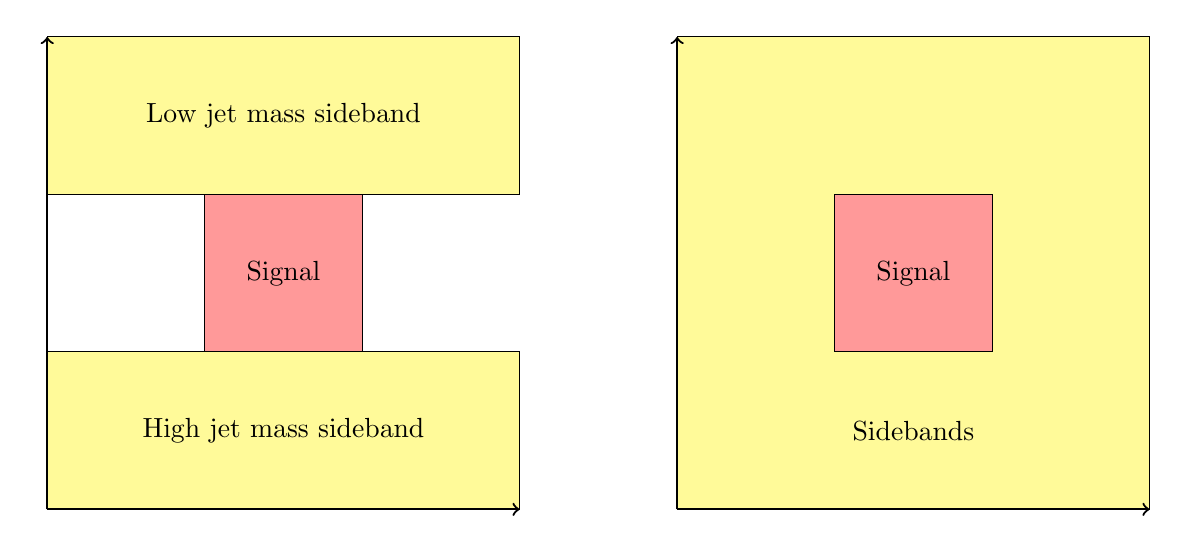
\begin{tikzpicture}
  % Jet mass sidebands
  \draw[fill=yellow!40] (0,0) rectangle (6,2) node[pos=0.5] {High jet mass sideband};
  \draw[fill=yellow!40] (0,4) rectangle (6,6) node[pos=0.5] {Low jet mass sideband};

  % Sidebands
  \draw[fill=yellow!40] (8,0) rectangle (14,6);
  \node at (11,1) {Sidebands};

  % Signal regions
  \draw[fill=red!40] (2,2) rectangle (4,4) node[pos=0.5] {Signal};
  \draw[fill=red!40] (10,2) rectangle (12,4) node[pos=0.5] {Signal};

  % Axes
  \draw[->,thick] (0,0) -- (6,0) node[below] {\MVV};
  \draw[->,thick] (0,0) -- (0,6) node[left] {\MJ};

  \draw[->,thick] (8,0) -- (14,0) node[below] {\MVV};
  \draw[->,thick] (8,0) -- (8,6) node[left] {\MJ};
\end{tikzpicture}

  \caption{
    Sideband regions of the fit for traditional sideband background estimation methods (left) versus the sideband regions in the 2D fit approach (right).
    The 2D fit method performs a simultaneous fit in the 2D sideband region in the \MVV-\MJ plane as opposed to modeling background in the \MVV and \MJ spectra in separate steps.
  }
  \label{fig:2Dfit}
\end{figure}

% Advantages of 2D fit
Thus, the 2D fit has the following advantages compared to the traditional $\alpha$ method previously used:
\begin{enumerate}
  \item The sideband as seen in figure~\ref{fig:2Dfit} is two-dimensional, thereby allowing for a simultaneous fit of the jet mass and resonance sidebands.
  This better constrains the background, which allows for better sensitivity of the search.
  \item The ability to add nuisance parameters that affect jet mass and resonance mass simultaneously, which allows us to account for the mismodeling of the correlation between the variables.
  \item Being able to use the full jet mass line-shape to extract the signal instead of using jet mass windows, providing better discrimination between $W$ and $Z$ peaks.
  \item Simultaneous fit of all \WV/\WH signals in the jet mass sideband, therefore allowing for easy implementation of exotic models such as heavy vector triplets.
\end{enumerate}

% Types of shapes in 2D fit
There are three types of shapes to consider for the 2D fit in the \MVV-\MJ plane.
The first is that of a signal process, for which we expect to see a resonance in both \MVV and \MJ.
In this case, the correlations are related to the scale and resolution of the jet.
For a background process in which there is a hadronically decaying boson (i.e., a $W$, $Z$, or $H$ from a \WVt process), we expect to observe a resonance in the \MJ dimension corresponding to the decay from the boson, but a falling spectrum in the \MVV dimension.
Lastly, if we instead have a QCD background process such as \Wjets, there will be a falling background distribution in both \MVV and \MJ, for which the shapes are correlated.

% Background types
As mentioned previously, two main classes of background are considered for this analysis, as classified based on resonant or non-resonant behavior in the \MJ spectrum:
\begin{itemize}
  \item \textbf{Resonant:} Background events in which the jet mass shape is peaking as a $W$, $Z$, $H$, or $t$ resonance in \MJ with a falling spectrum in \MVV.
  The resonant peak in \MJ is due to partially or fully merged top jets and diboson events in which one boosted boson is reconstructed into a jet.
  The main contribution is \WVt events.
  \item \textbf{Non-resonant:} Background events in which the jet is produced by the hadronization of one or more partons not originating from a vector boson.
  The dominant SM contribution is from \Wjets events, but additional contributions come from $t\bar{t}$ events as well.
\end{itemize}

% Merging samples for Run 2
The templates are derived from MC samples for both signal and background as enumerated in appendix~\ref{chap:appendixSamples}.
These samples were created in successive campaigns over 2016, 2017, and 2018, and are separated by their production year.
Previous versions of this analysis kept the templates separated by year, but for this iteration of the analysis we merge the samples for all three years and weight them by their respective luminosities to obtain combined Run 2 samples.
This has the benefit of providing better modeling of templates in categories with low statistics.

\subsection{Signal Modeling}
\label{sec:sig}

% Signal overview
Because the MC samples for the various signals used in the analysis only sample several points for the resonance mass \MX, we employ interpolation methods to model the signal for any arbitrary resonance mass \MX within the range 0.8-$4.5\unit{TeV}$.
To do so, we derive the each of the parameters for the signal shapes as functions of \MX, as well as the signal yield per pb of cross section as a function of \MX.

\subsubsection{Signal Shapes}

% Signal shapes
Each signal model takes the same functional form in the two-dimensional \MJ-\MVV space.
The signals are parameterized in 2D as the product of the two 1D \MJ and \MVV shapes for the jet mass and the resonance mass given by
\begin{equation}
  P_\mathrm{sig}(\MVV,\MJ|\MX)=\PVV(\MVV|\MX,\theta_1)\PJ(\MJ|\MX,\theta_2),
\end{equation}
where $\theta_1$ and $\theta_2$ are shape parameters that in principle depend on \MX.
Both shapes are modeled separately based on the jet purity (HP/LP), rapidity (HDy/LDy), and bb/nobb/vbf categories.
However, the $e$ and $\mu$ categories are merged for the signal modeling process.
To parameterize the shapes, we perform separate fits for the 1D shapes in the \MVV and \MJ spectra, then interpolate the parameters for each shape as a function of \MX to obtain $P_\mathrm{sig}(\MVV,\MJ|\MX)$ for arbitrary \MX between 1 and $4.5\unit{TeV}$.
A DCB shape is used for $\PVV(\MVV|\MX,\theta_1)$ for all categories, while the jet resonance shape $\PJ(\MJ|\MX,\theta_2)$ uses a DCB for the HP categories, and the sum of a DCB and an exponential for the LP categories.

% Signal shape parameter figures
Figures~\ref{fig:MVVShapes_NonVBF_LDy_Run2} and \ref{fig:MVVShapes_NonVBF_HDy_Run2} show the DCB parameters ($\mu$, $\sigma$, $\alpha_1$, $\alpha_2$) for the \MVV shapes in the 12 categories used to model the 2D signal shapes.
The DCB parameters for the \MJ shapes are shown in figures~\ref{fig:MJJShapeParam_LDy_Run2} and \ref{fig:MJJShapeParam_HDy_Run2}

% Signal shape substitutions
In some categories there are not enough events present that result in a smooth fit for the parameters of $\PVV(\MVV|\MX,\theta_1)$ or $\PJ(\MJ|\MX,\theta_2)$.
For example, signals that are \VBF-produced will not have a sufficient number of events present for the bb/nobb categories.
Because the signal parameters do not vary significantly between production modes, we allow for substituting non-\VBF signal shapes with \VBF shapes, and \VBF signal shapes with non-\VBF shapes:
\begin{itemize}
  \item \VBF\ZprtoWW shapes are used for \DY\ZprtoWW in the vbf categories.
  %\item \VBF\WprtoWH shapes are used for \DY\WprtoWH in the vbf categories.
  \item \VBF\WprtoWZ shapes are used for \DY\WprtoWZ in the vbf categories.
  \item \ggF\GBulktoWW shapes are used for \VBF\GBulktoWW in the bb categories.
  \item \DY\WprtoWZ shapes are used for \VBF\WprtoWZ in the bb and nobb categories.
  \item \ggF\RadtoWW shapes are used for \VBF\RadtoWW in the LP-bb categories.
  \item \ggF\GBulktoWW \MJ shapes are used for \DY\ZprtoWW \MJ in the LP-bb categories.
  \item \DY\ZprtoWW shapes are used for \VBF\ZprtoWW in the bb-LDy categories.
\end{itemize}

% Analytic signal shape figures
Figures \ref{fig:MVVShapes_NonVBF_LDy_Run2} and \ref{fig:MVVShapes_NonVBF_HDy_Run2} show the \MVV signal shapes for non-\VBF signals.
For figures \ref{fig:MVVShapes_VBF_LDy_Run2} and \ref{fig:MVVShapes_VBF_HDy_Run2}, we show the \MVV signal shapes for the \VBF signals.
In figures \ref{fig:MJJShapes_NonVBF_LDy_Run2} and \ref{fig:MJJShapes_NonVBF_LDy_Run2}, the \MJ signal shapes are shown for the non-\VBF signals.
Finally, figures \ref{fig:MJJShapes_VBF_LDy_Run2} and \ref{fig:MJJShapes_NonVBF_LDy_Run2} show the \MJ signal shapes for the \VBF signals.

\begin{figure}[htbp]
  \centering
  \includegraphics[width=0.2\textwidth]{fig/analysis/paramSignalShape_allSig_MVV_HP_bb_DEtaLo_MEAN.pdf}
  \includegraphics[width=0.2\textwidth]{fig/analysis/paramSignalShape_allSig_MVV_HP_bb_DEtaLo_SIGMA.pdf}
  \includegraphics[width=0.2\textwidth]{fig/analysis/paramSignalShape_allSig_MVV_HP_bb_DEtaLo_ALPHA1.pdf}
  \includegraphics[width=0.2\textwidth]{fig/analysis/paramSignalShape_allSig_MVV_HP_bb_DEtaLo_ALPHA2.pdf}\\
  \includegraphics[width=0.2\textwidth]{fig/analysis/paramSignalShape_allSig_MVV_LP_bb_DEtaLo_MEAN.pdf}
  \includegraphics[width=0.2\textwidth]{fig/analysis/paramSignalShape_allSig_MVV_LP_bb_DEtaLo_SIGMA.pdf}
  \includegraphics[width=0.2\textwidth]{fig/analysis/paramSignalShape_allSig_MVV_LP_bb_DEtaLo_ALPHA1.pdf}
  \includegraphics[width=0.2\textwidth]{fig/analysis/paramSignalShape_allSig_MVV_LP_bb_DEtaLo_ALPHA2.pdf}\\
  \includegraphics[width=0.2\textwidth]{fig/analysis/paramSignalShape_allSig_MVV_HP_nobb_DEtaLo_MEAN.pdf}
  \includegraphics[width=0.2\textwidth]{fig/analysis/paramSignalShape_allSig_MVV_HP_nobb_DEtaLo_SIGMA.pdf}
  \includegraphics[width=0.2\textwidth]{fig/analysis/paramSignalShape_allSig_MVV_HP_nobb_DEtaLo_ALPHA1.pdf}
  \includegraphics[width=0.2\textwidth]{fig/analysis/paramSignalShape_allSig_MVV_HP_nobb_DEtaLo_ALPHA2.pdf}\\
  \includegraphics[width=0.2\textwidth]{fig/analysis/paramSignalShape_allSig_MVV_LP_nobb_DEtaLo_MEAN.pdf}
  \includegraphics[width=0.2\textwidth]{fig/analysis/paramSignalShape_allSig_MVV_LP_nobb_DEtaLo_SIGMA.pdf}
  \includegraphics[width=0.2\textwidth]{fig/analysis/paramSignalShape_allSig_MVV_LP_nobb_DEtaLo_ALPHA1.pdf}
  \includegraphics[width=0.2\textwidth]{fig/analysis/paramSignalShape_allSig_MVV_LP_nobb_DEtaLo_ALPHA2.pdf}\\
  \includegraphics[width=0.2\textwidth]{fig/analysis/paramSignalShape_allSig_MVV_HP_vbf_DEtaLo_MEAN.pdf}
  \includegraphics[width=0.2\textwidth]{fig/analysis/paramSignalShape_allSig_MVV_HP_vbf_DEtaLo_SIGMA.pdf}
  \includegraphics[width=0.2\textwidth]{fig/analysis/paramSignalShape_allSig_MVV_HP_vbf_DEtaLo_ALPHA1.pdf}
  \includegraphics[width=0.2\textwidth]{fig/analysis/paramSignalShape_allSig_MVV_HP_vbf_DEtaLo_ALPHA2.pdf}\\
  \includegraphics[width=0.2\textwidth]{fig/analysis/paramSignalShape_allSig_MVV_LP_vbf_DEtaLo_MEAN.pdf}
  \includegraphics[width=0.2\textwidth]{fig/analysis/paramSignalShape_allSig_MVV_LP_vbf_DEtaLo_SIGMA.pdf}
  \includegraphics[width=0.2\textwidth]{fig/analysis/paramSignalShape_allSig_MVV_LP_vbf_DEtaLo_ALPHA1.pdf}
  \includegraphics[width=0.2\textwidth]{fig/analysis/paramSignalShape_allSig_MVV_LP_vbf_DEtaLo_ALPHA2.pdf}\\
  \caption{
    DCB parameters (from left to right: $\mu$, $\sigma$, $\alpha_1$, $\alpha_2$) for the diboson reconstructed mass \MVV as a function of \MX.
    Row 1: HP-bb-LDy, row 2: LP-bb-LDy, row 3: HP-nobb-LDy, row 4: LP-nobb-LDy, row 5: HP-vbf-LDy, row 6: LP-vbf-LDy.
  }
  \label{fig:MVVShapes_NonVBF_LDy_Run2}
\end{figure}

\begin{figure}[htbp]
  \centering
  \includegraphics[width=0.2\textwidth]{fig/analysis/paramSignalShape_allSig_MVV_HP_bb_DEtaHi_MEAN.pdf}
  \includegraphics[width=0.2\textwidth]{fig/analysis/paramSignalShape_allSig_MVV_HP_bb_DEtaHi_SIGMA.pdf}
  \includegraphics[width=0.2\textwidth]{fig/analysis/paramSignalShape_allSig_MVV_HP_bb_DEtaHi_ALPHA1.pdf}
  \includegraphics[width=0.2\textwidth]{fig/analysis/paramSignalShape_allSig_MVV_HP_bb_DEtaHi_ALPHA2.pdf}\\
  \includegraphics[width=0.2\textwidth]{fig/analysis/paramSignalShape_allSig_MVV_LP_bb_DEtaHi_MEAN.pdf}
  \includegraphics[width=0.2\textwidth]{fig/analysis/paramSignalShape_allSig_MVV_LP_bb_DEtaHi_SIGMA.pdf}
  \includegraphics[width=0.2\textwidth]{fig/analysis/paramSignalShape_allSig_MVV_LP_bb_DEtaHi_ALPHA1.pdf}
  \includegraphics[width=0.2\textwidth]{fig/analysis/paramSignalShape_allSig_MVV_LP_bb_DEtaHi_ALPHA2.pdf}\\
  \includegraphics[width=0.2\textwidth]{fig/analysis/paramSignalShape_allSig_MVV_HP_nobb_DEtaHi_MEAN.pdf}
  \includegraphics[width=0.2\textwidth]{fig/analysis/paramSignalShape_allSig_MVV_HP_nobb_DEtaHi_SIGMA.pdf}
  \includegraphics[width=0.2\textwidth]{fig/analysis/paramSignalShape_allSig_MVV_HP_nobb_DEtaHi_ALPHA1.pdf}
  \includegraphics[width=0.2\textwidth]{fig/analysis/paramSignalShape_allSig_MVV_HP_nobb_DEtaHi_ALPHA2.pdf}\\
  \includegraphics[width=0.2\textwidth]{fig/analysis/paramSignalShape_allSig_MVV_LP_nobb_DEtaHi_MEAN.pdf}
  \includegraphics[width=0.2\textwidth]{fig/analysis/paramSignalShape_allSig_MVV_LP_nobb_DEtaHi_SIGMA.pdf}
  \includegraphics[width=0.2\textwidth]{fig/analysis/paramSignalShape_allSig_MVV_LP_nobb_DEtaHi_ALPHA1.pdf}
  \includegraphics[width=0.2\textwidth]{fig/analysis/paramSignalShape_allSig_MVV_LP_nobb_DEtaHi_ALPHA2.pdf}\\
  \includegraphics[width=0.2\textwidth]{fig/analysis/paramSignalShape_allSig_MVV_HP_vbf_DEtaHi_MEAN.pdf}
  \includegraphics[width=0.2\textwidth]{fig/analysis/paramSignalShape_allSig_MVV_HP_vbf_DEtaHi_SIGMA.pdf}
  \includegraphics[width=0.2\textwidth]{fig/analysis/paramSignalShape_allSig_MVV_HP_vbf_DEtaHi_ALPHA1.pdf}
  \includegraphics[width=0.2\textwidth]{fig/analysis/paramSignalShape_allSig_MVV_HP_vbf_DEtaHi_ALPHA2.pdf}\\
  \includegraphics[width=0.2\textwidth]{fig/analysis/paramSignalShape_allSig_MVV_LP_vbf_DEtaHi_MEAN.pdf}
  \includegraphics[width=0.2\textwidth]{fig/analysis/paramSignalShape_allSig_MVV_LP_vbf_DEtaHi_SIGMA.pdf}
  \includegraphics[width=0.2\textwidth]{fig/analysis/paramSignalShape_allSig_MVV_LP_vbf_DEtaHi_ALPHA1.pdf}
  \includegraphics[width=0.2\textwidth]{fig/analysis/paramSignalShape_allSig_MVV_LP_vbf_DEtaHi_ALPHA2.pdf}\\
  \caption{
    DCB parameters (from left to right: $\mu$, $\sigma$, $\alpha_1$, $\alpha_2$) for the diboson reconstructed mass \MVV as a function of \MX.
    Row 1: HP-bb-HDy, row 2: LP-bb-HDy, row 3: HP-nobb-HDy, row 4: LP-nobb-HDy, row 5: HP-vbf-HDy, row 6: LP-vbf-HDy.
  }
  \label{fig:MVVShapes_NonVBF_HDy_Run2}
\end{figure}

\begin{figure}[htbp]
  \centering
  \includegraphics[width=0.2\textwidth]{fig/analysis/paramSignalShape_allSig_MJJ_HP_bb_DEtaLo_mean.pdf}
  \includegraphics[width=0.2\textwidth]{fig/analysis/paramSignalShape_allSig_MJJ_HP_bb_DEtaLo_sigma.pdf}
  \includegraphics[width=0.2\textwidth]{fig/analysis/paramSignalShape_allSig_MJJ_HP_bb_DEtaLo_alpha.pdf}
  \includegraphics[width=0.2\textwidth]{fig/analysis/paramSignalShape_allSig_MJJ_HP_bb_DEtaLo_alpha2.pdf}\\
  \includegraphics[width=0.2\textwidth]{fig/analysis/paramSignalShape_allSig_MJJ_LP_bb_DEtaLo_mean.pdf}
  \includegraphics[width=0.2\textwidth]{fig/analysis/paramSignalShape_allSig_MJJ_LP_bb_DEtaLo_sigma.pdf}
  \includegraphics[width=0.2\textwidth]{fig/analysis/paramSignalShape_allSig_MJJ_LP_bb_DEtaLo_alpha.pdf}
  \includegraphics[width=0.2\textwidth]{fig/analysis/paramSignalShape_allSig_MJJ_LP_bb_DEtaLo_alpha2.pdf}\\
  \includegraphics[width=0.2\textwidth]{fig/analysis/paramSignalShape_allSig_MJJ_HP_nobb_DEtaLo_mean.pdf}
  \includegraphics[width=0.2\textwidth]{fig/analysis/paramSignalShape_allSig_MJJ_HP_nobb_DEtaLo_sigma.pdf}
  \includegraphics[width=0.2\textwidth]{fig/analysis/paramSignalShape_allSig_MJJ_HP_nobb_DEtaLo_alpha.pdf}
  \includegraphics[width=0.2\textwidth]{fig/analysis/paramSignalShape_allSig_MJJ_HP_nobb_DEtaLo_alpha2.pdf}\\
  \includegraphics[width=0.2\textwidth]{fig/analysis/paramSignalShape_allSig_MJJ_LP_nobb_DEtaLo_mean.pdf}
  \includegraphics[width=0.2\textwidth]{fig/analysis/paramSignalShape_allSig_MJJ_LP_nobb_DEtaLo_sigma.pdf}
  \includegraphics[width=0.2\textwidth]{fig/analysis/paramSignalShape_allSig_MJJ_LP_nobb_DEtaLo_alpha.pdf}
  \includegraphics[width=0.2\textwidth]{fig/analysis/paramSignalShape_allSig_MJJ_LP_nobb_DEtaLo_alpha2.pdf}\\
  \includegraphics[width=0.2\textwidth]{fig/analysis/paramSignalShape_allSig_MJJ_HP_vbf_DEtaLo_mean.pdf}
  \includegraphics[width=0.2\textwidth]{fig/analysis/paramSignalShape_allSig_MJJ_HP_vbf_DEtaLo_sigma.pdf}
  \includegraphics[width=0.2\textwidth]{fig/analysis/paramSignalShape_allSig_MJJ_HP_vbf_DEtaLo_alpha.pdf}
  \includegraphics[width=0.2\textwidth]{fig/analysis/paramSignalShape_allSig_MJJ_HP_vbf_DEtaLo_alpha2.pdf}\\
  \includegraphics[width=0.2\textwidth]{fig/analysis/paramSignalShape_allSig_MJJ_LP_vbf_DEtaLo_mean.pdf}
  \includegraphics[width=0.2\textwidth]{fig/analysis/paramSignalShape_allSig_MJJ_LP_vbf_DEtaLo_sigma.pdf}
  \includegraphics[width=0.2\textwidth]{fig/analysis/paramSignalShape_allSig_MJJ_LP_vbf_DEtaLo_alpha.pdf}
  \includegraphics[width=0.2\textwidth]{fig/analysis/paramSignalShape_allSig_MJJ_LP_vbf_DEtaLo_alpha2.pdf}\\
  \caption{
    DCB parameters (from left to right: $\mu$, $\sigma$, $\alpha_1$, $\alpha_2$) for the jet mass \MJ as a function of \MX.
    Row 1: HP-bb-LDy, row 2: LP-bb-LDy, row 3: HP-nobb-LDy, row 4: LP-nobb-LDy, row 5: HP-vbf-LDy, row 6: LP-vbf-LDy.
  }
  \label{fig:MJJShapeParam_LDy_Run2}
\end{figure}

\begin{figure}[htbp]
  \centering
  \includegraphics[width=0.2\textwidth]{fig/analysis/paramSignalShape_allSig_MJJ_HP_bb_DEtaHi_mean.pdf}
  \includegraphics[width=0.2\textwidth]{fig/analysis/paramSignalShape_allSig_MJJ_HP_bb_DEtaHi_sigma.pdf}
  \includegraphics[width=0.2\textwidth]{fig/analysis/paramSignalShape_allSig_MJJ_HP_bb_DEtaHi_alpha.pdf}
  \includegraphics[width=0.2\textwidth]{fig/analysis/paramSignalShape_allSig_MJJ_HP_bb_DEtaHi_alpha2.pdf}\\
  \includegraphics[width=0.2\textwidth]{fig/analysis/paramSignalShape_allSig_MJJ_LP_bb_DEtaHi_mean.pdf}
  \includegraphics[width=0.2\textwidth]{fig/analysis/paramSignalShape_allSig_MJJ_LP_bb_DEtaHi_sigma.pdf}
  \includegraphics[width=0.2\textwidth]{fig/analysis/paramSignalShape_allSig_MJJ_LP_bb_DEtaHi_alpha.pdf}
  \includegraphics[width=0.2\textwidth]{fig/analysis/paramSignalShape_allSig_MJJ_LP_bb_DEtaHi_alpha2.pdf}\\
  \includegraphics[width=0.2\textwidth]{fig/analysis/paramSignalShape_allSig_MJJ_HP_nobb_DEtaHi_mean.pdf}
  \includegraphics[width=0.2\textwidth]{fig/analysis/paramSignalShape_allSig_MJJ_HP_nobb_DEtaHi_sigma.pdf}
  \includegraphics[width=0.2\textwidth]{fig/analysis/paramSignalShape_allSig_MJJ_HP_nobb_DEtaHi_alpha.pdf}
  \includegraphics[width=0.2\textwidth]{fig/analysis/paramSignalShape_allSig_MJJ_HP_nobb_DEtaHi_alpha2.pdf}\\
  \includegraphics[width=0.2\textwidth]{fig/analysis/paramSignalShape_allSig_MJJ_LP_nobb_DEtaHi_mean.pdf}
  \includegraphics[width=0.2\textwidth]{fig/analysis/paramSignalShape_allSig_MJJ_LP_nobb_DEtaHi_sigma.pdf}
  \includegraphics[width=0.2\textwidth]{fig/analysis/paramSignalShape_allSig_MJJ_LP_nobb_DEtaHi_alpha.pdf}
  \includegraphics[width=0.2\textwidth]{fig/analysis/paramSignalShape_allSig_MJJ_LP_nobb_DEtaHi_alpha2.pdf}\\
  \includegraphics[width=0.2\textwidth]{fig/analysis/paramSignalShape_allSig_MJJ_HP_vbf_DEtaHi_mean.pdf}
  \includegraphics[width=0.2\textwidth]{fig/analysis/paramSignalShape_allSig_MJJ_HP_vbf_DEtaHi_sigma.pdf}
  \includegraphics[width=0.2\textwidth]{fig/analysis/paramSignalShape_allSig_MJJ_HP_vbf_DEtaHi_alpha.pdf}
  \includegraphics[width=0.2\textwidth]{fig/analysis/paramSignalShape_allSig_MJJ_HP_vbf_DEtaHi_alpha2.pdf}\\
  \includegraphics[width=0.2\textwidth]{fig/analysis/paramSignalShape_allSig_MJJ_LP_vbf_DEtaHi_mean.pdf}
  \includegraphics[width=0.2\textwidth]{fig/analysis/paramSignalShape_allSig_MJJ_LP_vbf_DEtaHi_sigma.pdf}
  \includegraphics[width=0.2\textwidth]{fig/analysis/paramSignalShape_allSig_MJJ_LP_vbf_DEtaHi_alpha.pdf}
  \includegraphics[width=0.2\textwidth]{fig/analysis/paramSignalShape_allSig_MJJ_LP_vbf_DEtaHi_alpha2.pdf}\\
  \caption{
    DCB parameters (from left to right: $\mu$, $\sigma$, $\alpha_1$, $\alpha_2$) for the jet mass \MJ as a function of \MX.
    Row 1: HP-bb-HDy, row 2: LP-bb-HDy, row 3: HP-nobb-HDy, row 4: LP-nobb-HDy, row 5: HP-vbf-HDy, row 6: LP-vbf-HDy.
  }
  \label{fig:MJJShapeParam_HDy_Run2}
\end{figure}

\begin{figure}[htbp]
  \centering
  \includegraphics[width=0.18\textwidth]{fig/analysis/templateSignalVsMX_fromDC_GbuToWW_MVV_mu_HP_bb_DEtaLo.pdf}
  \includegraphics[width=0.18\textwidth]{fig/analysis/templateSignalVsMX_fromDC_RadToWW_MVV_mu_HP_bb_DEtaLo.pdf}
  \includegraphics[width=0.18\textwidth]{fig/analysis/templateSignalVsMX_fromDC_ZprToWW_MVV_mu_HP_bb_DEtaLo.pdf}
  \includegraphics[width=0.18\textwidth]{fig/analysis/templateSignalVsMX_fromDC_WprToWZ_MVV_mu_HP_bb_DEtaLo.pdf}
  \includegraphics[width=0.18\textwidth]{fig/analysis/templateSignalVsMX_fromDC_WprToWH_MVV_mu_HP_bb_DEtaLo.pdf}\\
  \includegraphics[width=0.18\textwidth]{fig/analysis/templateSignalVsMX_fromDC_GbuToWW_MVV_mu_LP_bb_DEtaLo.pdf}
  \includegraphics[width=0.18\textwidth]{fig/analysis/templateSignalVsMX_fromDC_RadToWW_MVV_mu_LP_bb_DEtaLo.pdf}
  \includegraphics[width=0.18\textwidth]{fig/analysis/templateSignalVsMX_fromDC_ZprToWW_MVV_mu_LP_bb_DEtaLo.pdf}
  \includegraphics[width=0.18\textwidth]{fig/analysis/templateSignalVsMX_fromDC_WprToWZ_MVV_mu_LP_bb_DEtaLo.pdf}
  \includegraphics[width=0.18\textwidth]{fig/analysis/templateSignalVsMX_fromDC_WprToWH_MVV_mu_LP_bb_DEtaLo.pdf}\\
  \includegraphics[width=0.18\textwidth]{fig/analysis/templateSignalVsMX_fromDC_GbuToWW_MVV_mu_HP_nobb_DEtaLo.pdf}
  \includegraphics[width=0.18\textwidth]{fig/analysis/templateSignalVsMX_fromDC_RadToWW_MVV_mu_HP_nobb_DEtaLo.pdf}
  \includegraphics[width=0.18\textwidth]{fig/analysis/templateSignalVsMX_fromDC_ZprToWW_MVV_mu_HP_nobb_DEtaLo.pdf}
  \includegraphics[width=0.18\textwidth]{fig/analysis/templateSignalVsMX_fromDC_WprToWZ_MVV_mu_HP_nobb_DEtaLo.pdf}
  \includegraphics[width=0.18\textwidth]{fig/analysis/templateSignalVsMX_fromDC_WprToWH_MVV_mu_HP_nobb_DEtaLo.pdf}\\
  \includegraphics[width=0.18\textwidth]{fig/analysis/templateSignalVsMX_fromDC_GbuToWW_MVV_mu_LP_nobb_DEtaLo.pdf}
  \includegraphics[width=0.18\textwidth]{fig/analysis/templateSignalVsMX_fromDC_RadToWW_MVV_mu_LP_nobb_DEtaLo.pdf}
  \includegraphics[width=0.18\textwidth]{fig/analysis/templateSignalVsMX_fromDC_ZprToWW_MVV_mu_LP_nobb_DEtaLo.pdf}
  \includegraphics[width=0.18\textwidth]{fig/analysis/templateSignalVsMX_fromDC_WprToWZ_MVV_mu_LP_nobb_DEtaLo.pdf}
  \includegraphics[width=0.18\textwidth]{fig/analysis/templateSignalVsMX_fromDC_WprToWH_MVV_mu_LP_nobb_DEtaLo.pdf}\\
  \includegraphics[width=0.18\textwidth]{fig/analysis/templateSignalVsMX_fromDC_GbuToWW_MVV_mu_HP_vbf_DEtaLo.pdf}
  \includegraphics[width=0.18\textwidth]{fig/analysis/templateSignalVsMX_fromDC_RadToWW_MVV_mu_HP_vbf_DEtaLo.pdf}
  \includegraphics[width=0.18\textwidth]{fig/analysis/templateSignalVsMX_fromDC_ZprToWW_MVV_mu_HP_vbf_DEtaLo.pdf}
  \includegraphics[width=0.18\textwidth]{fig/analysis/templateSignalVsMX_fromDC_WprToWZ_MVV_mu_HP_vbf_DEtaLo.pdf}
  \includegraphics[width=0.18\textwidth]{fig/analysis/templateSignalVsMX_fromDC_WprToWH_MVV_mu_HP_vbf_DEtaLo.pdf}\\
  \includegraphics[width=0.18\textwidth]{fig/analysis/templateSignalVsMX_fromDC_GbuToWW_MVV_mu_LP_vbf_DEtaLo.pdf}
  \includegraphics[width=0.18\textwidth]{fig/analysis/templateSignalVsMX_fromDC_RadToWW_MVV_mu_LP_vbf_DEtaLo.pdf}
  \includegraphics[width=0.18\textwidth]{fig/analysis/templateSignalVsMX_fromDC_ZprToWW_MVV_mu_LP_vbf_DEtaLo.pdf}
  \includegraphics[width=0.18\textwidth]{fig/analysis/templateSignalVsMX_fromDC_WprToWZ_MVV_mu_LP_vbf_DEtaLo.pdf}
  \includegraphics[width=0.18\textwidth]{fig/analysis/templateSignalVsMX_fromDC_WprToWH_MVV_mu_LP_vbf_DEtaLo.pdf}\\
  \caption{
    Signal shapes for the diboson reconstructed mass \MVV for \ggF- and \DY-produced signals, for 8 values of \MX.
    From left to right: \GBulktoWW, \RadtoWW, \ZprtoWW, \WprtoWZ, and \WprtoWH.
    Row 1: HP-bb-LDy, row 2: LP-bb-LDy, row 3: HP-nobb-LDy, row 4: LP-nobb-LDy, row 5: HP-vbf-LDy, row 6: LP-vbf-LDy.
  }
  \label{fig:MVVShapes_NonVBF_LDy_Run2}
\end{figure}

\begin{figure}[htbp]
  \centering
  \includegraphics[width=0.18\textwidth]{fig/analysis/templateSignalVsMX_fromDC_GbuToWW_MVV_mu_HP_bb_DEtaHi.pdf}
  \includegraphics[width=0.18\textwidth]{fig/analysis/templateSignalVsMX_fromDC_RadToWW_MVV_mu_HP_bb_DEtaHi.pdf}
  \includegraphics[width=0.18\textwidth]{fig/analysis/templateSignalVsMX_fromDC_ZprToWW_MVV_mu_HP_bb_DEtaHi.pdf}
  \includegraphics[width=0.18\textwidth]{fig/analysis/templateSignalVsMX_fromDC_WprToWZ_MVV_mu_HP_bb_DEtaHi.pdf}
  \includegraphics[width=0.18\textwidth]{fig/analysis/templateSignalVsMX_fromDC_WprToWH_MVV_mu_HP_bb_DEtaHi.pdf}\\
  \includegraphics[width=0.18\textwidth]{fig/analysis/templateSignalVsMX_fromDC_GbuToWW_MVV_mu_LP_bb_DEtaHi.pdf}
  \includegraphics[width=0.18\textwidth]{fig/analysis/templateSignalVsMX_fromDC_RadToWW_MVV_mu_LP_bb_DEtaHi.pdf}
  \includegraphics[width=0.18\textwidth]{fig/analysis/templateSignalVsMX_fromDC_ZprToWW_MVV_mu_LP_bb_DEtaHi.pdf}
  \includegraphics[width=0.18\textwidth]{fig/analysis/templateSignalVsMX_fromDC_WprToWZ_MVV_mu_LP_bb_DEtaHi.pdf}
  \includegraphics[width=0.18\textwidth]{fig/analysis/templateSignalVsMX_fromDC_WprToWH_MVV_mu_LP_bb_DEtaHi.pdf}\\
  \includegraphics[width=0.18\textwidth]{fig/analysis/templateSignalVsMX_fromDC_GbuToWW_MVV_mu_HP_nobb_DEtaHi.pdf}
  \includegraphics[width=0.18\textwidth]{fig/analysis/templateSignalVsMX_fromDC_RadToWW_MVV_mu_HP_nobb_DEtaHi.pdf}
  \includegraphics[width=0.18\textwidth]{fig/analysis/templateSignalVsMX_fromDC_ZprToWW_MVV_mu_HP_nobb_DEtaHi.pdf}
  \includegraphics[width=0.18\textwidth]{fig/analysis/templateSignalVsMX_fromDC_WprToWZ_MVV_mu_HP_nobb_DEtaHi.pdf}
  \includegraphics[width=0.18\textwidth]{fig/analysis/templateSignalVsMX_fromDC_WprToWH_MVV_mu_HP_nobb_DEtaHi.pdf}\\
  \includegraphics[width=0.18\textwidth]{fig/analysis/templateSignalVsMX_fromDC_GbuToWW_MVV_mu_LP_nobb_DEtaHi.pdf}
  \includegraphics[width=0.18\textwidth]{fig/analysis/templateSignalVsMX_fromDC_RadToWW_MVV_mu_LP_nobb_DEtaHi.pdf}
  \includegraphics[width=0.18\textwidth]{fig/analysis/templateSignalVsMX_fromDC_ZprToWW_MVV_mu_LP_nobb_DEtaHi.pdf}
  \includegraphics[width=0.18\textwidth]{fig/analysis/templateSignalVsMX_fromDC_WprToWZ_MVV_mu_LP_nobb_DEtaHi.pdf}
  \includegraphics[width=0.18\textwidth]{fig/analysis/templateSignalVsMX_fromDC_WprToWH_MVV_mu_LP_nobb_DEtaHi.pdf}\\
  \includegraphics[width=0.18\textwidth]{fig/analysis/templateSignalVsMX_fromDC_GbuToWW_MVV_mu_HP_vbf_DEtaHi.pdf}
  \includegraphics[width=0.18\textwidth]{fig/analysis/templateSignalVsMX_fromDC_RadToWW_MVV_mu_HP_vbf_DEtaHi.pdf}
  \includegraphics[width=0.18\textwidth]{fig/analysis/templateSignalVsMX_fromDC_ZprToWW_MVV_mu_HP_vbf_DEtaHi.pdf}
  \includegraphics[width=0.18\textwidth]{fig/analysis/templateSignalVsMX_fromDC_WprToWZ_MVV_mu_HP_vbf_DEtaHi.pdf}
  \includegraphics[width=0.18\textwidth]{fig/analysis/templateSignalVsMX_fromDC_WprToWH_MVV_mu_HP_vbf_DEtaHi.pdf}\\
  \includegraphics[width=0.18\textwidth]{fig/analysis/templateSignalVsMX_fromDC_GbuToWW_MVV_mu_LP_vbf_DEtaHi.pdf}
  \includegraphics[width=0.18\textwidth]{fig/analysis/templateSignalVsMX_fromDC_RadToWW_MVV_mu_LP_vbf_DEtaHi.pdf}
  \includegraphics[width=0.18\textwidth]{fig/analysis/templateSignalVsMX_fromDC_ZprToWW_MVV_mu_LP_vbf_DEtaHi.pdf}
  \includegraphics[width=0.18\textwidth]{fig/analysis/templateSignalVsMX_fromDC_WprToWZ_MVV_mu_LP_vbf_DEtaHi.pdf}
  \includegraphics[width=0.18\textwidth]{fig/analysis/templateSignalVsMX_fromDC_WprToWH_MVV_mu_LP_vbf_DEtaHi.pdf}\\
  \caption{
    Signal shapes for the diboson reconstructed mass \MVV for \ggF- and \DY-produced signals, for 8 values of \MX.
    From left to right: \GBulktoWW, \RadtoWW, \ZprtoWW, \WprtoWZ, and \WprtoWH.
    Row 1: HP-bb-HDy, row 2: LP-bb-HDy, row 3: HP-nobb-HDy, row 4: LP-nobb-HDy, row 5: HP-vbf-HDy, row 6: LP-vbf-HDy.
  }
  \label{fig:MVVShapes_NonVBF_HDy_Run2}
\end{figure}

\begin{figure}[htbp]
  \centering
  \includegraphics[width=0.18\textwidth]{fig/analysis/templateSignalVsMX_fromDC_VBFGbuToWW_MVV_mu_HP_bb_DEtaLo.pdf}
  \includegraphics[width=0.18\textwidth]{fig/analysis/templateSignalVsMX_fromDC_VBFRadToWW_MVV_mu_HP_bb_DEtaLo.pdf}
  \includegraphics[width=0.18\textwidth]{fig/analysis/templateSignalVsMX_fromDC_VBFZprToWW_MVV_mu_HP_bb_DEtaLo.pdf}
  \includegraphics[width=0.18\textwidth]{fig/analysis/templateSignalVsMX_fromDC_VBFWprToWZ_MVV_mu_HP_bb_DEtaLo.pdf}\\
  \includegraphics[width=0.18\textwidth]{fig/analysis/templateSignalVsMX_fromDC_VBFGbuToWW_MVV_mu_LP_bb_DEtaLo.pdf}
  \includegraphics[width=0.18\textwidth]{fig/analysis/templateSignalVsMX_fromDC_VBFRadToWW_MVV_mu_LP_bb_DEtaLo.pdf}
  \includegraphics[width=0.18\textwidth]{fig/analysis/templateSignalVsMX_fromDC_VBFZprToWW_MVV_mu_LP_bb_DEtaLo.pdf}
  \includegraphics[width=0.18\textwidth]{fig/analysis/templateSignalVsMX_fromDC_VBFWprToWZ_MVV_mu_LP_bb_DEtaLo.pdf}\\
  \includegraphics[width=0.18\textwidth]{fig/analysis/templateSignalVsMX_fromDC_VBFGbuToWW_MVV_mu_HP_nobb_DEtaLo.pdf}
  \includegraphics[width=0.18\textwidth]{fig/analysis/templateSignalVsMX_fromDC_VBFRadToWW_MVV_mu_HP_nobb_DEtaLo.pdf}
  \includegraphics[width=0.18\textwidth]{fig/analysis/templateSignalVsMX_fromDC_VBFZprToWW_MVV_mu_HP_nobb_DEtaLo.pdf}
  \includegraphics[width=0.18\textwidth]{fig/analysis/templateSignalVsMX_fromDC_VBFWprToWZ_MVV_mu_HP_nobb_DEtaLo.pdf}\\
  \includegraphics[width=0.18\textwidth]{fig/analysis/templateSignalVsMX_fromDC_VBFGbuToWW_MVV_mu_LP_nobb_DEtaLo.pdf}
  \includegraphics[width=0.18\textwidth]{fig/analysis/templateSignalVsMX_fromDC_VBFRadToWW_MVV_mu_LP_nobb_DEtaLo.pdf}
  \includegraphics[width=0.18\textwidth]{fig/analysis/templateSignalVsMX_fromDC_VBFZprToWW_MVV_mu_LP_nobb_DEtaLo.pdf}
  \includegraphics[width=0.18\textwidth]{fig/analysis/templateSignalVsMX_fromDC_VBFWprToWZ_MVV_mu_LP_nobb_DEtaLo.pdf}\\
  \includegraphics[width=0.18\textwidth]{fig/analysis/templateSignalVsMX_fromDC_VBFGbuToWW_MVV_mu_HP_vbf_DEtaLo.pdf}
  \includegraphics[width=0.18\textwidth]{fig/analysis/templateSignalVsMX_fromDC_VBFRadToWW_MVV_mu_HP_vbf_DEtaLo.pdf}
  \includegraphics[width=0.18\textwidth]{fig/analysis/templateSignalVsMX_fromDC_VBFZprToWW_MVV_mu_HP_vbf_DEtaLo.pdf}
  \includegraphics[width=0.18\textwidth]{fig/analysis/templateSignalVsMX_fromDC_VBFWprToWZ_MVV_mu_HP_vbf_DEtaLo.pdf}\\
  \includegraphics[width=0.18\textwidth]{fig/analysis/templateSignalVsMX_fromDC_VBFGbuToWW_MVV_mu_LP_vbf_DEtaLo.pdf}
  \includegraphics[width=0.18\textwidth]{fig/analysis/templateSignalVsMX_fromDC_VBFRadToWW_MVV_mu_LP_vbf_DEtaLo.pdf}
  \includegraphics[width=0.18\textwidth]{fig/analysis/templateSignalVsMX_fromDC_VBFZprToWW_MVV_mu_LP_vbf_DEtaLo.pdf}
  \includegraphics[width=0.18\textwidth]{fig/analysis/templateSignalVsMX_fromDC_VBFWprToWZ_MVV_mu_LP_vbf_DEtaLo.pdf}\\
  \caption{
    Signal shapes for the diboson reconstructed mass \MVV for \VBF-produced signals, for 8 values of \MX.
    From left to right: \GBulktoWW, \RadtoWW, \ZprtoWW, and \WprtoWZ.
    Row 1: HP-bb-LDy, row 2: LP-bb-LDy, row 3: HP-nobb-LDy, row 4: LP-nobb-LDy, row 5: HP-vbf-LDy, row 6: LP-vbf-LDy.
  }
  \label{fig:MVVShapes_VBF_LDy_Run2}
\end{figure}

\begin{figure}[htbp]
  \centering
  \includegraphics[width=0.18\textwidth]{fig/analysis/templateSignalVsMX_fromDC_VBFGbuToWW_MVV_mu_HP_bb_DEtaHi.pdf}
  \includegraphics[width=0.18\textwidth]{fig/analysis/templateSignalVsMX_fromDC_VBFRadToWW_MVV_mu_HP_bb_DEtaHi.pdf}
  \includegraphics[width=0.18\textwidth]{fig/analysis/templateSignalVsMX_fromDC_VBFZprToWW_MVV_mu_HP_bb_DEtaHi.pdf}
  \includegraphics[width=0.18\textwidth]{fig/analysis/templateSignalVsMX_fromDC_VBFWprToWZ_MVV_mu_HP_bb_DEtaHi.pdf}\\
  \includegraphics[width=0.18\textwidth]{fig/analysis/templateSignalVsMX_fromDC_VBFGbuToWW_MVV_mu_LP_bb_DEtaHi.pdf}
  \includegraphics[width=0.18\textwidth]{fig/analysis/templateSignalVsMX_fromDC_VBFRadToWW_MVV_mu_LP_bb_DEtaHi.pdf}
  \includegraphics[width=0.18\textwidth]{fig/analysis/templateSignalVsMX_fromDC_VBFZprToWW_MVV_mu_LP_bb_DEtaHi.pdf}
  \includegraphics[width=0.18\textwidth]{fig/analysis/templateSignalVsMX_fromDC_VBFWprToWZ_MVV_mu_LP_bb_DEtaHi.pdf}\\
  \includegraphics[width=0.18\textwidth]{fig/analysis/templateSignalVsMX_fromDC_VBFGbuToWW_MVV_mu_HP_nobb_DEtaHi.pdf}
  \includegraphics[width=0.18\textwidth]{fig/analysis/templateSignalVsMX_fromDC_VBFRadToWW_MVV_mu_HP_nobb_DEtaHi.pdf}
  \includegraphics[width=0.18\textwidth]{fig/analysis/templateSignalVsMX_fromDC_VBFZprToWW_MVV_mu_HP_nobb_DEtaHi.pdf}
  \includegraphics[width=0.18\textwidth]{fig/analysis/templateSignalVsMX_fromDC_VBFWprToWZ_MVV_mu_HP_nobb_DEtaHi.pdf}\\
  \includegraphics[width=0.18\textwidth]{fig/analysis/templateSignalVsMX_fromDC_VBFGbuToWW_MVV_mu_LP_nobb_DEtaHi.pdf}
  \includegraphics[width=0.18\textwidth]{fig/analysis/templateSignalVsMX_fromDC_VBFRadToWW_MVV_mu_LP_nobb_DEtaHi.pdf}
  \includegraphics[width=0.18\textwidth]{fig/analysis/templateSignalVsMX_fromDC_VBFZprToWW_MVV_mu_LP_nobb_DEtaHi.pdf}
  \includegraphics[width=0.18\textwidth]{fig/analysis/templateSignalVsMX_fromDC_VBFWprToWZ_MVV_mu_LP_nobb_DEtaHi.pdf}\\
  \includegraphics[width=0.18\textwidth]{fig/analysis/templateSignalVsMX_fromDC_VBFGbuToWW_MVV_mu_HP_vbf_DEtaHi.pdf}
  \includegraphics[width=0.18\textwidth]{fig/analysis/templateSignalVsMX_fromDC_VBFRadToWW_MVV_mu_HP_vbf_DEtaHi.pdf}
  \includegraphics[width=0.18\textwidth]{fig/analysis/templateSignalVsMX_fromDC_VBFZprToWW_MVV_mu_HP_vbf_DEtaHi.pdf}
  \includegraphics[width=0.18\textwidth]{fig/analysis/templateSignalVsMX_fromDC_VBFWprToWZ_MVV_mu_HP_vbf_DEtaHi.pdf}\\
  \includegraphics[width=0.18\textwidth]{fig/analysis/templateSignalVsMX_fromDC_VBFGbuToWW_MVV_mu_LP_vbf_DEtaHi.pdf}
  \includegraphics[width=0.18\textwidth]{fig/analysis/templateSignalVsMX_fromDC_VBFRadToWW_MVV_mu_LP_vbf_DEtaHi.pdf}
  \includegraphics[width=0.18\textwidth]{fig/analysis/templateSignalVsMX_fromDC_VBFZprToWW_MVV_mu_LP_vbf_DEtaHi.pdf}
  \includegraphics[width=0.18\textwidth]{fig/analysis/templateSignalVsMX_fromDC_VBFWprToWZ_MVV_mu_LP_vbf_DEtaHi.pdf}\\
  \caption{
    Signal shapes for the diboson reconstructed mass \MVV for \VBF-produced signals, for 8 values of \MX.
    From left to right: \GBulktoWW, \RadtoWW, \ZprtoWW, and \WprtoWZ.
    Row 1: HP-bb-HDy, row 2: LP-bb-HDy, row 3: HP-nobb-HDy, row 4: LP-nobb-HDy, row 5: HP-vbf-HDy, row 6: LP-vbf-HDy.
  }
  \label{fig:MVVShapes_VBF_HDy_Run2}
\end{figure}

\begin{figure}[htbp]
  \centering
  \includegraphics[width=0.18\textwidth]{fig/analysis/templateSignalVsMX_fromDC_GbuToWW_MJJ_mu_HP_bb_DEtaLo.pdf}
  \includegraphics[width=0.18\textwidth]{fig/analysis/templateSignalVsMX_fromDC_RadToWW_MJJ_mu_HP_bb_DEtaLo.pdf}
  \includegraphics[width=0.18\textwidth]{fig/analysis/templateSignalVsMX_fromDC_ZprToWW_MJJ_mu_HP_bb_DEtaLo.pdf}
  \includegraphics[width=0.18\textwidth]{fig/analysis/templateSignalVsMX_fromDC_WprToWZ_MJJ_mu_HP_bb_DEtaLo.pdf}
  \includegraphics[width=0.18\textwidth]{fig/analysis/templateSignalVsMX_fromDC_WprToWH_MJJ_mu_HP_bb_DEtaLo.pdf}\\
  \includegraphics[width=0.18\textwidth]{fig/analysis/templateSignalVsMX_fromDC_GbuToWW_MJJ_mu_LP_bb_DEtaLo.pdf}
  \includegraphics[width=0.18\textwidth]{fig/analysis/templateSignalVsMX_fromDC_RadToWW_MJJ_mu_LP_bb_DEtaLo.pdf}
  \includegraphics[width=0.18\textwidth]{fig/analysis/templateSignalVsMX_fromDC_ZprToWW_MJJ_mu_LP_bb_DEtaLo.pdf}
  \includegraphics[width=0.18\textwidth]{fig/analysis/templateSignalVsMX_fromDC_WprToWZ_MJJ_mu_LP_bb_DEtaLo.pdf}
  \includegraphics[width=0.18\textwidth]{fig/analysis/templateSignalVsMX_fromDC_WprToWH_MJJ_mu_LP_bb_DEtaLo.pdf}\\
  \includegraphics[width=0.18\textwidth]{fig/analysis/templateSignalVsMX_fromDC_GbuToWW_MJJ_mu_HP_nobb_DEtaLo.pdf}
  \includegraphics[width=0.18\textwidth]{fig/analysis/templateSignalVsMX_fromDC_RadToWW_MJJ_mu_HP_nobb_DEtaLo.pdf}
  \includegraphics[width=0.18\textwidth]{fig/analysis/templateSignalVsMX_fromDC_ZprToWW_MJJ_mu_HP_nobb_DEtaLo.pdf}
  \includegraphics[width=0.18\textwidth]{fig/analysis/templateSignalVsMX_fromDC_WprToWZ_MJJ_mu_HP_nobb_DEtaLo.pdf}
  \includegraphics[width=0.18\textwidth]{fig/analysis/templateSignalVsMX_fromDC_WprToWH_MJJ_mu_HP_nobb_DEtaLo.pdf}\\
  \includegraphics[width=0.18\textwidth]{fig/analysis/templateSignalVsMX_fromDC_GbuToWW_MJJ_mu_LP_nobb_DEtaLo.pdf}
  \includegraphics[width=0.18\textwidth]{fig/analysis/templateSignalVsMX_fromDC_RadToWW_MJJ_mu_LP_nobb_DEtaLo.pdf}
  \includegraphics[width=0.18\textwidth]{fig/analysis/templateSignalVsMX_fromDC_ZprToWW_MJJ_mu_LP_nobb_DEtaLo.pdf}
  \includegraphics[width=0.18\textwidth]{fig/analysis/templateSignalVsMX_fromDC_WprToWZ_MJJ_mu_LP_nobb_DEtaLo.pdf}
  \includegraphics[width=0.18\textwidth]{fig/analysis/templateSignalVsMX_fromDC_WprToWH_MJJ_mu_LP_nobb_DEtaLo.pdf}\\
  \includegraphics[width=0.18\textwidth]{fig/analysis/templateSignalVsMX_fromDC_GbuToWW_MJJ_mu_HP_vbf_DEtaLo.pdf}
  \includegraphics[width=0.18\textwidth]{fig/analysis/templateSignalVsMX_fromDC_RadToWW_MJJ_mu_HP_vbf_DEtaLo.pdf}
  \includegraphics[width=0.18\textwidth]{fig/analysis/templateSignalVsMX_fromDC_ZprToWW_MJJ_mu_HP_vbf_DEtaLo.pdf}
  \includegraphics[width=0.18\textwidth]{fig/analysis/templateSignalVsMX_fromDC_WprToWZ_MJJ_mu_HP_vbf_DEtaLo.pdf}
  \includegraphics[width=0.18\textwidth]{fig/analysis/templateSignalVsMX_fromDC_WprToWH_MJJ_mu_HP_vbf_DEtaLo.pdf}\\
  \includegraphics[width=0.18\textwidth]{fig/analysis/templateSignalVsMX_fromDC_GbuToWW_MJJ_mu_LP_vbf_DEtaLo.pdf}
  \includegraphics[width=0.18\textwidth]{fig/analysis/templateSignalVsMX_fromDC_RadToWW_MJJ_mu_LP_vbf_DEtaLo.pdf}
  \includegraphics[width=0.18\textwidth]{fig/analysis/templateSignalVsMX_fromDC_ZprToWW_MJJ_mu_LP_vbf_DEtaLo.pdf}
  \includegraphics[width=0.18\textwidth]{fig/analysis/templateSignalVsMX_fromDC_WprToWZ_MJJ_mu_LP_vbf_DEtaLo.pdf}
  \includegraphics[width=0.18\textwidth]{fig/analysis/templateSignalVsMX_fromDC_WprToWH_MJJ_mu_LP_vbf_DEtaLo.pdf}\\
  \caption{
    Signal shapes for the soft drop jet mass \MJ for \ggF- and \DY-produced signals, for 8 values of \MX.
    From left to right: \GBulktoWW, \RadtoWW, \ZprtoWW, \WprtoWZ, and \WprtoWH.
    Row 1: HP-bb-LDy, row 2: LP-bb-LDy, row 3: HP-nobb-LDy, row 4: LP-nobb-LDy, row 5: HP-vbf-LDy, row 6: LP-vbf-LDy.
  }
  \label{fig:MJJShapes_NonVBF_LDy_Run2}
\end{figure}

\begin{figure}[htbp]
  \centering
  \includegraphics[width=0.18\textwidth]{fig/analysis/templateSignalVsMX_fromDC_GbuToWW_MJJ_mu_HP_bb_DEtaHi.pdf}
  \includegraphics[width=0.18\textwidth]{fig/analysis/templateSignalVsMX_fromDC_RadToWW_MJJ_mu_HP_bb_DEtaHi.pdf}
  \includegraphics[width=0.18\textwidth]{fig/analysis/templateSignalVsMX_fromDC_ZprToWW_MJJ_mu_HP_bb_DEtaHi.pdf}
  \includegraphics[width=0.18\textwidth]{fig/analysis/templateSignalVsMX_fromDC_WprToWZ_MJJ_mu_HP_bb_DEtaHi.pdf}
  \includegraphics[width=0.18\textwidth]{fig/analysis/templateSignalVsMX_fromDC_WprToWH_MJJ_mu_HP_bb_DEtaHi.pdf}\\
  \includegraphics[width=0.18\textwidth]{fig/analysis/templateSignalVsMX_fromDC_GbuToWW_MJJ_mu_LP_bb_DEtaHi.pdf}
  \includegraphics[width=0.18\textwidth]{fig/analysis/templateSignalVsMX_fromDC_RadToWW_MJJ_mu_LP_bb_DEtaHi.pdf}
  \includegraphics[width=0.18\textwidth]{fig/analysis/templateSignalVsMX_fromDC_ZprToWW_MJJ_mu_LP_bb_DEtaHi.pdf}
  \includegraphics[width=0.18\textwidth]{fig/analysis/templateSignalVsMX_fromDC_WprToWZ_MJJ_mu_LP_bb_DEtaHi.pdf}
  \includegraphics[width=0.18\textwidth]{fig/analysis/templateSignalVsMX_fromDC_WprToWH_MJJ_mu_LP_bb_DEtaHi.pdf}\\
  \includegraphics[width=0.18\textwidth]{fig/analysis/templateSignalVsMX_fromDC_GbuToWW_MJJ_mu_HP_nobb_DEtaHi.pdf}
  \includegraphics[width=0.18\textwidth]{fig/analysis/templateSignalVsMX_fromDC_RadToWW_MJJ_mu_HP_nobb_DEtaHi.pdf}
  \includegraphics[width=0.18\textwidth]{fig/analysis/templateSignalVsMX_fromDC_ZprToWW_MJJ_mu_HP_nobb_DEtaHi.pdf}
  \includegraphics[width=0.18\textwidth]{fig/analysis/templateSignalVsMX_fromDC_WprToWZ_MJJ_mu_HP_nobb_DEtaHi.pdf}
  \includegraphics[width=0.18\textwidth]{fig/analysis/templateSignalVsMX_fromDC_WprToWH_MJJ_mu_HP_nobb_DEtaHi.pdf}\\
  \includegraphics[width=0.18\textwidth]{fig/analysis/templateSignalVsMX_fromDC_GbuToWW_MJJ_mu_LP_nobb_DEtaHi.pdf}
  \includegraphics[width=0.18\textwidth]{fig/analysis/templateSignalVsMX_fromDC_RadToWW_MJJ_mu_LP_nobb_DEtaHi.pdf}
  \includegraphics[width=0.18\textwidth]{fig/analysis/templateSignalVsMX_fromDC_ZprToWW_MJJ_mu_LP_nobb_DEtaHi.pdf}
  \includegraphics[width=0.18\textwidth]{fig/analysis/templateSignalVsMX_fromDC_WprToWZ_MJJ_mu_LP_nobb_DEtaHi.pdf}
  \includegraphics[width=0.18\textwidth]{fig/analysis/templateSignalVsMX_fromDC_WprToWH_MJJ_mu_LP_nobb_DEtaHi.pdf}\\
  \includegraphics[width=0.18\textwidth]{fig/analysis/templateSignalVsMX_fromDC_GbuToWW_MJJ_mu_HP_vbf_DEtaHi.pdf}
  \includegraphics[width=0.18\textwidth]{fig/analysis/templateSignalVsMX_fromDC_RadToWW_MJJ_mu_HP_vbf_DEtaHi.pdf}
  \includegraphics[width=0.18\textwidth]{fig/analysis/templateSignalVsMX_fromDC_ZprToWW_MJJ_mu_HP_vbf_DEtaHi.pdf}
  \includegraphics[width=0.18\textwidth]{fig/analysis/templateSignalVsMX_fromDC_WprToWZ_MJJ_mu_HP_vbf_DEtaHi.pdf}
  \includegraphics[width=0.18\textwidth]{fig/analysis/templateSignalVsMX_fromDC_WprToWH_MJJ_mu_HP_vbf_DEtaHi.pdf}\\
  \includegraphics[width=0.18\textwidth]{fig/analysis/templateSignalVsMX_fromDC_GbuToWW_MJJ_mu_LP_vbf_DEtaHi.pdf}
  \includegraphics[width=0.18\textwidth]{fig/analysis/templateSignalVsMX_fromDC_RadToWW_MJJ_mu_LP_vbf_DEtaHi.pdf}
  \includegraphics[width=0.18\textwidth]{fig/analysis/templateSignalVsMX_fromDC_ZprToWW_MJJ_mu_LP_vbf_DEtaHi.pdf}
  \includegraphics[width=0.18\textwidth]{fig/analysis/templateSignalVsMX_fromDC_WprToWZ_MJJ_mu_LP_vbf_DEtaHi.pdf}
  \includegraphics[width=0.18\textwidth]{fig/analysis/templateSignalVsMX_fromDC_WprToWH_MJJ_mu_LP_vbf_DEtaHi.pdf}\\
  \caption{
    Signal shapes for the soft drop jet mass \MJ for \ggF- and \DY-produced signals, for 8 values of \MX.
    From left to right: \GBulktoWW, \RadtoWW, \ZprtoWW, \WprtoWZ, and \WprtoWH.
    Row 1: HP-bb-HDy, row 2: LP-bb-HDy, row 3: HP-nobb-HDy, row 4: LP-nobb-HDy, row 5: HP-vbf-HDy, row 6: LP-vbf-HDy.
  }
  \label{fig:MJJShapes_NonVBF_HDy_Run2}
\end{figure}

\begin{figure}[htbp]
  \centering
  \includegraphics[width=0.18\textwidth]{fig/analysis/templateSignalVsMX_fromDC_VBFGbuToWW_MJJ_mu_HP_bb_DEtaLo.pdf}
  \includegraphics[width=0.18\textwidth]{fig/analysis/templateSignalVsMX_fromDC_VBFRadToWW_MJJ_mu_HP_bb_DEtaLo.pdf}
  \includegraphics[width=0.18\textwidth]{fig/analysis/templateSignalVsMX_fromDC_VBFZprToWW_MJJ_mu_HP_bb_DEtaLo.pdf}
  \includegraphics[width=0.18\textwidth]{fig/analysis/templateSignalVsMX_fromDC_VBFWprToWZ_MJJ_mu_HP_bb_DEtaLo.pdf}\\
  \includegraphics[width=0.18\textwidth]{fig/analysis/templateSignalVsMX_fromDC_VBFGbuToWW_MJJ_mu_LP_bb_DEtaLo.pdf}
  \includegraphics[width=0.18\textwidth]{fig/analysis/templateSignalVsMX_fromDC_VBFRadToWW_MJJ_mu_LP_bb_DEtaLo.pdf}
  \includegraphics[width=0.18\textwidth]{fig/analysis/templateSignalVsMX_fromDC_VBFZprToWW_MJJ_mu_LP_bb_DEtaLo.pdf}
  \includegraphics[width=0.18\textwidth]{fig/analysis/templateSignalVsMX_fromDC_VBFWprToWZ_MJJ_mu_LP_bb_DEtaLo.pdf}\\
  \includegraphics[width=0.18\textwidth]{fig/analysis/templateSignalVsMX_fromDC_VBFGbuToWW_MJJ_mu_HP_nobb_DEtaLo.pdf}
  \includegraphics[width=0.18\textwidth]{fig/analysis/templateSignalVsMX_fromDC_VBFRadToWW_MJJ_mu_HP_nobb_DEtaLo.pdf}
  \includegraphics[width=0.18\textwidth]{fig/analysis/templateSignalVsMX_fromDC_VBFZprToWW_MJJ_mu_HP_nobb_DEtaLo.pdf}
  \includegraphics[width=0.18\textwidth]{fig/analysis/templateSignalVsMX_fromDC_VBFWprToWZ_MJJ_mu_HP_nobb_DEtaLo.pdf}\\
  \includegraphics[width=0.18\textwidth]{fig/analysis/templateSignalVsMX_fromDC_VBFGbuToWW_MJJ_mu_LP_nobb_DEtaLo.pdf}
  \includegraphics[width=0.18\textwidth]{fig/analysis/templateSignalVsMX_fromDC_VBFRadToWW_MJJ_mu_LP_nobb_DEtaLo.pdf}
  \includegraphics[width=0.18\textwidth]{fig/analysis/templateSignalVsMX_fromDC_VBFZprToWW_MJJ_mu_LP_nobb_DEtaLo.pdf}
  \includegraphics[width=0.18\textwidth]{fig/analysis/templateSignalVsMX_fromDC_VBFWprToWZ_MJJ_mu_LP_nobb_DEtaLo.pdf}\\
  \includegraphics[width=0.18\textwidth]{fig/analysis/templateSignalVsMX_fromDC_VBFGbuToWW_MJJ_mu_HP_vbf_DEtaLo.pdf}
  \includegraphics[width=0.18\textwidth]{fig/analysis/templateSignalVsMX_fromDC_VBFRadToWW_MJJ_mu_HP_vbf_DEtaLo.pdf}
  \includegraphics[width=0.18\textwidth]{fig/analysis/templateSignalVsMX_fromDC_VBFZprToWW_MJJ_mu_HP_vbf_DEtaLo.pdf}
  \includegraphics[width=0.18\textwidth]{fig/analysis/templateSignalVsMX_fromDC_VBFWprToWZ_MJJ_mu_HP_vbf_DEtaLo.pdf}\\
  \includegraphics[width=0.18\textwidth]{fig/analysis/templateSignalVsMX_fromDC_VBFGbuToWW_MJJ_mu_LP_vbf_DEtaLo.pdf}
  \includegraphics[width=0.18\textwidth]{fig/analysis/templateSignalVsMX_fromDC_VBFRadToWW_MJJ_mu_LP_vbf_DEtaLo.pdf}
  \includegraphics[width=0.18\textwidth]{fig/analysis/templateSignalVsMX_fromDC_VBFZprToWW_MJJ_mu_LP_vbf_DEtaLo.pdf}
  \includegraphics[width=0.18\textwidth]{fig/analysis/templateSignalVsMX_fromDC_VBFWprToWZ_MJJ_mu_LP_vbf_DEtaLo.pdf}\\
  \caption{
    Signal shapes for the soft drop jet mass \MJ for \VBF-produced signals, for 8 values of \MX.
    From left to right: \GBulktoWW, \RadtoWW, \ZprtoWW, and \WprtoWZ.
    Row 1: HP-bb-LDy, row 2: LP-bb-LDy, row 3: HP-nobb-LDy, row 4: LP-nobb-LDy, row 5: HP-vbf-LDy, row 6: LP-vbf-LDy.
  }
  \label{fig:MJJShapes_VBF_LDy_Run2}
\end{figure}

\begin{figure}[htbp]
  \centering
  \includegraphics[width=0.18\textwidth]{fig/analysis/templateSignalVsMX_fromDC_VBFGbuToWW_MJJ_mu_HP_bb_DEtaHi.pdf}
  \includegraphics[width=0.18\textwidth]{fig/analysis/templateSignalVsMX_fromDC_VBFRadToWW_MJJ_mu_HP_bb_DEtaHi.pdf}
  \includegraphics[width=0.18\textwidth]{fig/analysis/templateSignalVsMX_fromDC_VBFZprToWW_MJJ_mu_HP_bb_DEtaHi.pdf}
  \includegraphics[width=0.18\textwidth]{fig/analysis/templateSignalVsMX_fromDC_VBFWprToWZ_MJJ_mu_HP_bb_DEtaHi.pdf}\\
  \includegraphics[width=0.18\textwidth]{fig/analysis/templateSignalVsMX_fromDC_VBFGbuToWW_MJJ_mu_LP_bb_DEtaHi.pdf}
  \includegraphics[width=0.18\textwidth]{fig/analysis/templateSignalVsMX_fromDC_VBFRadToWW_MJJ_mu_LP_bb_DEtaHi.pdf}
  \includegraphics[width=0.18\textwidth]{fig/analysis/templateSignalVsMX_fromDC_VBFZprToWW_MJJ_mu_LP_bb_DEtaHi.pdf}
  \includegraphics[width=0.18\textwidth]{fig/analysis/templateSignalVsMX_fromDC_VBFWprToWZ_MJJ_mu_LP_bb_DEtaHi.pdf}\\
  \includegraphics[width=0.18\textwidth]{fig/analysis/templateSignalVsMX_fromDC_VBFGbuToWW_MJJ_mu_HP_nobb_DEtaHi.pdf}
  \includegraphics[width=0.18\textwidth]{fig/analysis/templateSignalVsMX_fromDC_VBFRadToWW_MJJ_mu_HP_nobb_DEtaHi.pdf}
  \includegraphics[width=0.18\textwidth]{fig/analysis/templateSignalVsMX_fromDC_VBFZprToWW_MJJ_mu_HP_nobb_DEtaHi.pdf}
  \includegraphics[width=0.18\textwidth]{fig/analysis/templateSignalVsMX_fromDC_VBFWprToWZ_MJJ_mu_HP_nobb_DEtaHi.pdf}\\
  \includegraphics[width=0.18\textwidth]{fig/analysis/templateSignalVsMX_fromDC_VBFGbuToWW_MJJ_mu_LP_nobb_DEtaHi.pdf}
  \includegraphics[width=0.18\textwidth]{fig/analysis/templateSignalVsMX_fromDC_VBFRadToWW_MJJ_mu_LP_nobb_DEtaHi.pdf}
  \includegraphics[width=0.18\textwidth]{fig/analysis/templateSignalVsMX_fromDC_VBFZprToWW_MJJ_mu_LP_nobb_DEtaHi.pdf}
  \includegraphics[width=0.18\textwidth]{fig/analysis/templateSignalVsMX_fromDC_VBFWprToWZ_MJJ_mu_LP_nobb_DEtaHi.pdf}\\
  \includegraphics[width=0.18\textwidth]{fig/analysis/templateSignalVsMX_fromDC_VBFGbuToWW_MJJ_mu_HP_vbf_DEtaHi.pdf}
  \includegraphics[width=0.18\textwidth]{fig/analysis/templateSignalVsMX_fromDC_VBFRadToWW_MJJ_mu_HP_vbf_DEtaHi.pdf}
  \includegraphics[width=0.18\textwidth]{fig/analysis/templateSignalVsMX_fromDC_VBFZprToWW_MJJ_mu_HP_vbf_DEtaHi.pdf}
  \includegraphics[width=0.18\textwidth]{fig/analysis/templateSignalVsMX_fromDC_VBFWprToWZ_MJJ_mu_HP_vbf_DEtaHi.pdf}\\
  \includegraphics[width=0.18\textwidth]{fig/analysis/templateSignalVsMX_fromDC_VBFGbuToWW_MJJ_mu_LP_vbf_DEtaHi.pdf}
  \includegraphics[width=0.18\textwidth]{fig/analysis/templateSignalVsMX_fromDC_VBFRadToWW_MJJ_mu_LP_vbf_DEtaHi.pdf}
  \includegraphics[width=0.18\textwidth]{fig/analysis/templateSignalVsMX_fromDC_VBFZprToWW_MJJ_mu_LP_vbf_DEtaHi.pdf}
  \includegraphics[width=0.18\textwidth]{fig/analysis/templateSignalVsMX_fromDC_VBFWprToWZ_MJJ_mu_LP_vbf_DEtaHi.pdf}\\
  \caption{
    Signal shapes for the soft drop jet mass \MJ for \VBF-produced signals, for 8 values of \MX.
    From left to right: \GBulktoWW, \RadtoWW, \ZprtoWW, and \WprtoWZ.
    Row 1: HP-bb-HDy, row 2: LP-bb-HDy, row 3: HP-nobb-HDy, row 4: LP-nobb-HDy, row 5: HP-vbf-HDy, row 6: LP-vbf-HDy.
  }
  \label{fig:MJJShapes_VBF_HDy_Run2}
\end{figure}

\subsubsection{Signal Yields}

% Signal yields
The process for parameterizing the signal yield as a function of \MX is similar to obtaining the parameters for the signal shapes.
We compute the yield per pb of cross section for each mass point from our signal MC samples, then fit the result with a polynomial interpolation to obtain a function of \MX.
Figures~\ref{fig:YieldParam_NonVBF_Run2} and \ref{fig:YieldParam_VBF_Run2} show the expected yields per pb of cross section for non-\VBF and \VBF signals, respectively.

\begin{figure}[htbp]
  \centering
  \includegraphics[width=0.2\textwidth]{fig/analysis/paramSignalYield_NonVBFSig_mu_HP_bb_DEtaLo.pdf}
  \includegraphics[width=0.2\textwidth]{fig/analysis/paramSignalYield_NonVBFSig_e_HP_bb_DEtaLo.pdf}
  \includegraphics[width=0.2\textwidth]{fig/analysis/paramSignalYield_NonVBFSig_mu_LP_bb_DEtaLo.pdf}
  \includegraphics[width=0.2\textwidth]{fig/analysis/paramSignalYield_NonVBFSig_e_LP_bb_DEtaLo.pdf}\\
  \includegraphics[width=0.2\textwidth]{fig/analysis/paramSignalYield_NonVBFSig_mu_HP_nobb_DEtaLo.pdf}
  \includegraphics[width=0.2\textwidth]{fig/analysis/paramSignalYield_NonVBFSig_e_HP_nobb_DEtaLo.pdf}
  \includegraphics[width=0.2\textwidth]{fig/analysis/paramSignalYield_NonVBFSig_mu_LP_nobb_DEtaLo.pdf}
  \includegraphics[width=0.2\textwidth]{fig/analysis/paramSignalYield_NonVBFSig_e_LP_nobb_DEtaLo.pdf}\\
  \includegraphics[width=0.2\textwidth]{fig/analysis/paramSignalYield_NonVBFSig_mu_HP_vbf_DEtaLo.pdf}
  \includegraphics[width=0.2\textwidth]{fig/analysis/paramSignalYield_NonVBFSig_e_HP_vbf_DEtaLo.pdf}
  \includegraphics[width=0.2\textwidth]{fig/analysis/paramSignalYield_NonVBFSig_mu_LP_vbf_DEtaLo.pdf}
  \includegraphics[width=0.2\textwidth]{fig/analysis/paramSignalYield_NonVBFSig_e_LP_vbf_DEtaLo.pdf}\\
  \includegraphics[width=0.2\textwidth]{fig/analysis/paramSignalYield_NonVBFSig_mu_HP_bb_DEtaHi.pdf}
  \includegraphics[width=0.2\textwidth]{fig/analysis/paramSignalYield_NonVBFSig_e_HP_bb_DEtaHi.pdf}
  \includegraphics[width=0.2\textwidth]{fig/analysis/paramSignalYield_NonVBFSig_mu_LP_bb_DEtaHi.pdf}
  \includegraphics[width=0.2\textwidth]{fig/analysis/paramSignalYield_NonVBFSig_e_LP_bb_DEtaHi.pdf}\\
  \includegraphics[width=0.2\textwidth]{fig/analysis/paramSignalYield_NonVBFSig_mu_HP_nobb_DEtaHi.pdf}
  \includegraphics[width=0.2\textwidth]{fig/analysis/paramSignalYield_NonVBFSig_e_HP_nobb_DEtaHi.pdf}
  \includegraphics[width=0.2\textwidth]{fig/analysis/paramSignalYield_NonVBFSig_mu_LP_nobb_DEtaHi.pdf}
  \includegraphics[width=0.2\textwidth]{fig/analysis/paramSignalYield_NonVBFSig_e_LP_nobb_DEtaHi.pdf}\\
  \includegraphics[width=0.2\textwidth]{fig/analysis/paramSignalYield_NonVBFSig_mu_HP_vbf_DEtaHi.pdf}
  \includegraphics[width=0.2\textwidth]{fig/analysis/paramSignalYield_NonVBFSig_e_HP_vbf_DEtaHi.pdf}
  \includegraphics[width=0.2\textwidth]{fig/analysis/paramSignalYield_NonVBFSig_mu_LP_vbf_DEtaHi.pdf}
  \includegraphics[width=0.2\textwidth]{fig/analysis/paramSignalYield_NonVBFSig_e_LP_vbf_DEtaHi.pdf}\\
  \caption{
    Parameterizations of the expected yields per pb of cross section for \ggF- and \DY-produced signals as a function of \MX.
    Columns 1 to 4: $\mu$-HP, e-HP, $\mu$-LP, and e-LP.
    Rows 1 to 6: bb-LDy, nobb-LDy, vbf-LDy, bb-HDy, nobb-HDy, and vbf-HDy.}
  \label{fig:YieldParam_NonVBF_Run2}
\end{figure}

\begin{figure}[htbp]
  \centering
  \includegraphics[width=0.2\textwidth]{fig/analysis/paramSignalYield_VBFSig_mu_HP_bb_DEtaLo.pdf}
  \includegraphics[width=0.2\textwidth]{fig/analysis/paramSignalYield_VBFSig_e_HP_bb_DEtaLo.pdf}
  \includegraphics[width=0.2\textwidth]{fig/analysis/paramSignalYield_VBFSig_mu_LP_bb_DEtaLo.pdf}
  \includegraphics[width=0.2\textwidth]{fig/analysis/paramSignalYield_VBFSig_e_LP_bb_DEtaLo.pdf}\\
  \includegraphics[width=0.2\textwidth]{fig/analysis/paramSignalYield_VBFSig_mu_HP_nobb_DEtaLo.pdf}
  \includegraphics[width=0.2\textwidth]{fig/analysis/paramSignalYield_VBFSig_e_HP_nobb_DEtaLo.pdf}
  \includegraphics[width=0.2\textwidth]{fig/analysis/paramSignalYield_VBFSig_mu_LP_nobb_DEtaLo.pdf}
  \includegraphics[width=0.2\textwidth]{fig/analysis/paramSignalYield_VBFSig_e_LP_nobb_DEtaLo.pdf}\\
  \includegraphics[width=0.2\textwidth]{fig/analysis/paramSignalYield_VBFSig_mu_HP_vbf_DEtaLo.pdf}
  \includegraphics[width=0.2\textwidth]{fig/analysis/paramSignalYield_VBFSig_e_HP_vbf_DEtaLo.pdf}
  \includegraphics[width=0.2\textwidth]{fig/analysis/paramSignalYield_VBFSig_mu_LP_vbf_DEtaLo.pdf}
  \includegraphics[width=0.2\textwidth]{fig/analysis/paramSignalYield_VBFSig_e_LP_vbf_DEtaLo.pdf}\\
  \includegraphics[width=0.2\textwidth]{fig/analysis/paramSignalYield_VBFSig_mu_HP_bb_DEtaHi.pdf}
  \includegraphics[width=0.2\textwidth]{fig/analysis/paramSignalYield_VBFSig_e_HP_bb_DEtaHi.pdf}
  \includegraphics[width=0.2\textwidth]{fig/analysis/paramSignalYield_VBFSig_mu_LP_bb_DEtaHi.pdf}
  \includegraphics[width=0.2\textwidth]{fig/analysis/paramSignalYield_VBFSig_e_LP_bb_DEtaHi.pdf}\\
  \includegraphics[width=0.2\textwidth]{fig/analysis/paramSignalYield_VBFSig_mu_HP_nobb_DEtaHi.pdf}
  \includegraphics[width=0.2\textwidth]{fig/analysis/paramSignalYield_VBFSig_e_HP_nobb_DEtaHi.pdf}
  \includegraphics[width=0.2\textwidth]{fig/analysis/paramSignalYield_VBFSig_mu_LP_nobb_DEtaHi.pdf}
  \includegraphics[width=0.2\textwidth]{fig/analysis/paramSignalYield_VBFSig_e_LP_nobb_DEtaHi.pdf}\\
  \includegraphics[width=0.2\textwidth]{fig/analysis/paramSignalYield_VBFSig_mu_HP_vbf_DEtaHi.pdf}
  \includegraphics[width=0.2\textwidth]{fig/analysis/paramSignalYield_VBFSig_e_HP_vbf_DEtaHi.pdf}
  \includegraphics[width=0.2\textwidth]{fig/analysis/paramSignalYield_VBFSig_mu_LP_vbf_DEtaHi.pdf}
  \includegraphics[width=0.2\textwidth]{fig/analysis/paramSignalYield_VBFSig_e_LP_vbf_DEtaHi.pdf}\\
  \caption{
    Parameterizations of the expected yields per pb of cross section for \VBF-produced signals as a function of \MX.
    Columns 1 to 4: $\mu$-HP, e-HP, $\mu$-LP, and e-LP.
    Rows 1 to 6: bb-LDy, nobb-LDy, vbf-LDy, bb-HDy, nobb-HDy, and vbf-HDy.}
  \label{fig:YieldParam_VBF_Run2}
\end{figure}

\subsection{Background Modeling}
\label{sec:bkg}

% Background template overview
Unlike the signal shapes described in the previous section, both the resonant and non-resonant background modeling involve 2D histograms rather than smooth shapes.
This is in part due to the challenges encountered with the modeling process, which is a result of the low statistics for the background MC samples after applying the selection cuts.

\subsubsection{Non-resonant Background Templates}

% Non-resonant background templates overview
The non-resonant background templates are modeled with conditional products, taking the form
\begin{equation}
  P_{\Wjets}(\MVV,\MJ)=\PVV(\MVV|\MJ,\theta_1)\PJ(\MJ|\theta_2).
\end{equation}
For $\PJ(\MJ|\theta_2)$ we derive a 1D template for the \MJ distribution, which we then multiply with a 2D shape from $\PVV(\MVV|\MJ,\theta_1)$ for the \MVV distribution.

% 2D conditional template
For the 2D \MVV shape, we use a specialized Gaussian kernel method in order overcome the low statistics encountered for the background MC events.
Standard Gaussian methods were found to be ineffective at capturing peaks in the 2D plane, as they would result in a smearing of the peaks from reconstructed simulation events.
To remedy this, we employ a method in which we use a partially generated diboson invariant mass \MVVpart, which is defined as the four vector sum of the reconstructed \Wlep, and a generated jet.
The generated jet is made by clustering generated particle candidates with $\Delta R<1.2$ around reconstructed jets using the anti-\kt algorithm with a distance parameter of $R=0.8$.

% Response function
Because the generated jets are used in place of the reconstructed \Vhad, we must make use of a detector response function to accurately model reconstruction of the simulated jets.
This is done in simulation by estimating the Gaussian mean and sigma of the resolution of $\MVV/\MVVpart$ in bins of generator jet \pt, which can be seen in figure~\ref{fig:nonResScaleResMVV}.
We then begin generating the template by populating the \MJ spectrum using a coarse binning.
For each event in a slice of the \MJ spectrum, we add a 1D Gaussian onto the partial mass with scale shifted by the detector response and width equal to the Gaussian resolution as defined by
\begin{equation}\label{eq:Pplus}
  P_+=\frac{w_i}{\sqrt{2\pi}\sigma}\exp\bqty{-\frac{1}{2}\pqty{\frac{x-s\MVVpart}{\sigma}}^2},
\end{equation}
where $w_i$ is the event weight, and $s$ and $\sigma$ are the scale and resolution parameters obtained from the detector response.

\begin{figure}[htbp]
  \centering
  \includegraphics[width=0.4\textwidth]{fig/analysis/detectorParam_nonRes_scale_MVV.pdf}
  \includegraphics[width=0.4\textwidth]{fig/analysis/detectorParam_nonRes_resolution_MVV.pdf}
  \caption{
    Scale (left) and resolution (right) of \MVV as a function of the generated jet \pt.
  }
  \label{fig:nonResScaleResMVV}
\end{figure}

% Template smoothing
Another issue encountered with the low statistics of the MC samples is the lack of events at higher values of \MVV.
To address this, we perform a smoothing of the tails of the \MVV shape with a power law function in each bin of \MJ.
We then populate the 2D histogram with values from the \MVV shape in each \MJ bin, with the power law functions sampled from $1.2\unit{TeV}$ and onward for the bb categories, and $1.6\unit{TeV}$ and onward for the nobb categories.

% Template conditionality
To ensure that the template is conditional with respect to \MJ, each histogram slice corresponding to one crude bin of \MJ is normalized.
We then interpolate over the coarsely binned \MJ histogram for each \MVV bin using a spline, which is used to populate the 2D histogram.
As a final step, we normalize each \MJ slice again to ensure the conditionality of the template.

% Merged categories
Ideally, this process of generating the 2D conditional templates would be done for all 24 categories as defined in subsection~\ref{subsec:eventCat}.
However, this is met with more difficulties due to the low statistics provided by the MC samples.
To resolve this issue, we merge categories together based on whether or not they exhibit similar behavior.
We consider various metrics of behavior between categories, such as the correlation between \MJ and \MVV, as well as the average jet \pt as a function of the jet mass, which is shown in figure~\ref{fig:nonRes2DCorr} between the four combinations of HP/LP and nobb/bb categories.
The behavior is similar enough between the categories that they may be considered for merging.
For this analysis, we merge the $e$/$\mu$ and bb/nobb/vbf categories while keeping the HP/LP and HDy/LDy categories separate, for a total of four 2D conditional templates.

\begin{figure}[htbp]
  \centering
  \includegraphics[width=0.45\textwidth]{fig/analysis/nonRes_corr.pdf}
  \caption{
    Average \pt of the jet as a function of the jet mass \MJ compared between the four combinations of HP/LP and nobb/bb categories for the non-resonant background MC samples.
  }
  \label{fig:nonRes2DCorr}
\end{figure}

% Reweighting templates
Prior to creating the 2D conditional templates, a reweighting procedure is applied in the jet mass sideband region for the \MVV spectrum in order to ensure that the templates accurately capture the behavior of the background events.
We again merge the $e$ and $\mu$ categories for this process due to their similar behavior, but for other categories such as nobb/bb/vbf, we derive separate weighting functions for the \MVV spectrum.
The categories are then merged to create the four conditional 2D templates after the weighting process.
The reweighting function takes the form $f(\MVV)=a+b/\MVV$ to ensure that the weights behave as expected in the asymptotic limit, and the fit coefficients are derived by fitting the function to the ratio of data to MC.
From this we obtain the weights $w_i$ of equation~\ref{eq:Pplus}.
Figure~\ref{fig:nonResMvvSpectrumReweighting} shows the \MVV distributions from which the weights are derived.

\begin{figure}[htbp]
  \centering
  \includegraphics[width=0.2\textwidth]{fig/analysis/slopesSB_b1_allL_HP_bb_LDy_Run2_mWV_1OverX.pdf}
  \includegraphics[width=0.2\textwidth]{fig/analysis/slopesSB_b1_allL_LP_bb_LDy_Run2_mWV_1OverX.pdf}
  \includegraphics[width=0.2\textwidth]{fig/analysis/slopesSB_b1_allL_HP_bb_HDy_Run2_mWV_1OverX.pdf}
  \includegraphics[width=0.2\textwidth]{fig/analysis/slopesSB_b1_allL_LP_bb_HDy_Run2_mWV_1OverX.pdf}\\
  \includegraphics[width=0.2\textwidth]{fig/analysis/slopesSB_b1_allL_HP_nobb_LDy_Run2_mWV_1OverX.pdf}
  \includegraphics[width=0.2\textwidth]{fig/analysis/slopesSB_b1_allL_LP_nobb_LDy_Run2_mWV_1OverX.pdf}
  \includegraphics[width=0.2\textwidth]{fig/analysis/slopesSB_b1_allL_HP_nobb_HDy_Run2_mWV_1OverX.pdf}
  \includegraphics[width=0.2\textwidth]{fig/analysis/slopesSB_b1_allL_LP_nobb_HDy_Run2_mWV_1OverX.pdf}\\
  \includegraphics[width=0.2\textwidth]{fig/analysis/slopesSB_b1_allL_HP_vbf_LDy_Run2_mWV_1OverX.pdf}
  \includegraphics[width=0.2\textwidth]{fig/analysis/slopesSB_b1_allL_LP_vbf_LDy_Run2_mWV_1OverX.pdf}
  \includegraphics[width=0.2\textwidth]{fig/analysis/slopesSB_b1_allL_HP_vbf_HDy_Run2_mWV_1OverX.pdf}
  \includegraphics[width=0.2\textwidth]{fig/analysis/slopesSB_b1_allL_LP_vbf_HDy_Run2_mWV_1OverX.pdf}\\
  \caption{
    Plots of the \MVV spectra for the full Run 2 data and MC samples in the jet mass sideband for each category, with the $e$ and $\mu$ categories merged.
    After merging the $e$ and $\mu$ categories, the remaining categories are kept separate and the ratio of data to MC is fitted with a function of the form $f(\MVV)=a+b/\MVV$.
    The resulting weights for each event $w_i$ are then used in equation~\ref{eq:Pplus} when building the conditional 2D templates.
    Columns 1 to 4: HP-LDy, LP-LDy, HP-HDy, and LP-HDy.
    Rows 1 to 3: bb, nobb, and vbf for data, but with merged bb+nobb+vbf distributions for the MC.
  }
  \label{fig:nonResMvvSpectrumReweighting}
\end{figure}

% Non-resonant closure test
As a check on the closure of the 2D conditional template building process, we plot the projection of the templates on the \MVV spectrum versus the weighted MC distributions.
Figure~\ref{fig:condTemplateVscondReco_nonRes_MVV_Run2} shows the resulting comparison between the templates and the MC samples for each of the four merged categories, which show good agreement between each other.

\begin{figure}[htbp]
  \centering
  \includegraphics[width=0.45\textwidth]{fig/analysis/templateVsReco_nonResCond_MVV_e_HP_nobb_LDy.pdf}
  \includegraphics[width=0.45\textwidth]{fig/analysis/templateVsReco_nonResCond_MVV_e_HP_nobb_HDy.pdf}\\
  \includegraphics[width=0.45\textwidth]{fig/analysis/templateVsReco_nonResCond_MVV_e_LP_nobb_LDy.pdf}
  \includegraphics[width=0.45\textwidth]{fig/analysis/templateVsReco_nonResCond_MVV_e_LP_nobb_HDy.pdf}\\
  \caption{
    Projection onto the \MVV spectrum of the 2D conditional non-resonant background templates (solid lines) versus the weighted MC distributions (points) used to make them, for the HP-LDy (top left), HP-HDy (top right), LP-LDy (bottom left), and LP-HDy (bottom right) merged categories.
    Four separate \MJ ranges are plotted, with one corresponding to the full \MJ range, and three corresponding to the sub-ranges.
  }
  \label{fig:condTemplateVscondReco_nonRes_MVV_Run2}
\end{figure}

% 1D non-resonant soft drop jet mass templates
The remaining step to complete the conditional product $P_{\Wjets}(\MVV,\MJ)$ is to obtain the 1D template for $\PJ(\MJ|\theta_2)$.
Rather than using a kernel method as with the 2D conditional template, we instead use a coarsely binned histogram of weighted MC events for \MJ, and then fit the result with a spline.
The spline is then used to interpolate the $\PJ(\MJ|\theta_2)$ template with the final \MJ binning.
In this case, we also do not merge any of the 24 categories and keep the templates separate.
Figure~\ref{fig:1dtemplateVsReco_nonRes_MJ_Run2} shows the resulting 1D templates for each category compared to the weighted MC distributions used to obtain them.

\begin{figure}[htbp]
  \centering
  \includegraphics[width=0.2\textwidth]{fig/analysis/templateVsReco_nonRes_r0_MJ_mu_HP_bb_LDy.pdf}
  \includegraphics[width=0.2\textwidth]{fig/analysis/templateVsReco_nonRes_r0_MJ_e_HP_bb_LDy.pdf}
  \includegraphics[width=0.2\textwidth]{fig/analysis/templateVsReco_nonRes_r0_MJ_mu_LP_bb_LDy.pdf}
  \includegraphics[width=0.2\textwidth]{fig/analysis/templateVsReco_nonRes_r0_MJ_e_LP_bb_LDy.pdf}\\
  \includegraphics[width=0.2\textwidth]{fig/analysis/templateVsReco_nonRes_r0_MJ_mu_HP_nobb_LDy.pdf}
  \includegraphics[width=0.2\textwidth]{fig/analysis/templateVsReco_nonRes_r0_MJ_e_HP_nobb_LDy.pdf}
  \includegraphics[width=0.2\textwidth]{fig/analysis/templateVsReco_nonRes_r0_MJ_mu_LP_nobb_LDy.pdf}
  \includegraphics[width=0.2\textwidth]{fig/analysis/templateVsReco_nonRes_r0_MJ_e_LP_nobb_LDy.pdf}\\
  \includegraphics[width=0.2\textwidth]{fig/analysis/templateVsReco_nonRes_r0_MJ_mu_HP_vbf_LDy.pdf}
  \includegraphics[width=0.2\textwidth]{fig/analysis/templateVsReco_nonRes_r0_MJ_e_HP_vbf_LDy.pdf}
  \includegraphics[width=0.2\textwidth]{fig/analysis/templateVsReco_nonRes_r0_MJ_mu_LP_vbf_LDy.pdf}
  \includegraphics[width=0.2\textwidth]{fig/analysis/templateVsReco_nonRes_r0_MJ_e_LP_vbf_LDy.pdf}\\
  \includegraphics[width=0.2\textwidth]{fig/analysis/templateVsReco_nonRes_r0_MJ_mu_HP_bb_HDy.pdf}
  \includegraphics[width=0.2\textwidth]{fig/analysis/templateVsReco_nonRes_r0_MJ_e_HP_bb_HDy.pdf}
  \includegraphics[width=0.2\textwidth]{fig/analysis/templateVsReco_nonRes_r0_MJ_mu_LP_bb_HDy.pdf}
  \includegraphics[width=0.2\textwidth]{fig/analysis/templateVsReco_nonRes_r0_MJ_e_LP_bb_HDy.pdf}\\
  \includegraphics[width=0.2\textwidth]{fig/analysis/templateVsReco_nonRes_r0_MJ_mu_HP_nobb_HDy.pdf}
  \includegraphics[width=0.2\textwidth]{fig/analysis/templateVsReco_nonRes_r0_MJ_e_HP_nobb_HDy.pdf}
  \includegraphics[width=0.2\textwidth]{fig/analysis/templateVsReco_nonRes_r0_MJ_mu_LP_nobb_HDy.pdf}
  \includegraphics[width=0.2\textwidth]{fig/analysis/templateVsReco_nonRes_r0_MJ_e_LP_nobb_HDy.pdf}\\
  \includegraphics[width=0.2\textwidth]{fig/analysis/templateVsReco_nonRes_r0_MJ_mu_HP_vbf_HDy.pdf}
  \includegraphics[width=0.2\textwidth]{fig/analysis/templateVsReco_nonRes_r0_MJ_e_HP_vbf_HDy.pdf}
  \includegraphics[width=0.2\textwidth]{fig/analysis/templateVsReco_nonRes_r0_MJ_mu_LP_vbf_HDy.pdf}
  \includegraphics[width=0.2\textwidth]{fig/analysis/templateVsReco_nonRes_r0_MJ_e_LP_vbf_HDy.pdf}\\
  \caption{
    Comparison of the 1D \MJ templates for the non-resonant background (solid line) and the weighted MC distributions (points).
    Columns 1 to 4: $\mu$-HP, $e$-HP, $\mu$-LP, and $e$-LP.
    Rows 1 to 6: bb-LDy, nobb-LDy, vbf-LDy, bb-HDy, nobb-HDy, and vbf-HDy.
  }
  \label{fig:1dtemplateVsReco_nonRes_MJ_Run2}
\end{figure}

% Final non-resonant templates
The final non-resonant templates are then obtained from the product of the 2D conditional template with the 1D jet mass shape.
Figure~\ref{fig:templates_nonRes_Run2} shows the 2D templates for each of the 24 categories.
To better visualize the differences between each of the categories, figure~\ref{fig:compTemplate_nonRes} shows comparisons of the \MVV and \MJ projections of the templates for each category.

\begin{figure}[htbp]
  \centering
  \includegraphics[width=0.2\textwidth]{fig/analysis/template_nonRes_mu_HP_bb_LDy.pdf}
  \includegraphics[width=0.2\textwidth]{fig/analysis/template_nonRes_e_HP_bb_LDy.pdf}
  \includegraphics[width=0.2\textwidth]{fig/analysis/template_nonRes_mu_LP_bb_LDy.pdf}
  \includegraphics[width=0.2\textwidth]{fig/analysis/template_nonRes_e_LP_bb_LDy.pdf}\\
  \includegraphics[width=0.2\textwidth]{fig/analysis/template_nonRes_mu_HP_nobb_LDy.pdf}
  \includegraphics[width=0.2\textwidth]{fig/analysis/template_nonRes_e_HP_nobb_LDy.pdf}
  \includegraphics[width=0.2\textwidth]{fig/analysis/template_nonRes_mu_LP_nobb_LDy.pdf}
  \includegraphics[width=0.2\textwidth]{fig/analysis/template_nonRes_e_LP_nobb_LDy.pdf}\\
  \includegraphics[width=0.2\textwidth]{fig/analysis/template_nonRes_mu_HP_vbf_LDy.pdf}
  \includegraphics[width=0.2\textwidth]{fig/analysis/template_nonRes_e_HP_vbf_LDy.pdf}
  \includegraphics[width=0.2\textwidth]{fig/analysis/template_nonRes_mu_LP_vbf_LDy.pdf}
  \includegraphics[width=0.2\textwidth]{fig/analysis/template_nonRes_e_LP_vbf_LDy.pdf}\\
  \includegraphics[width=0.2\textwidth]{fig/analysis/template_nonRes_mu_HP_bb_HDy.pdf}
  \includegraphics[width=0.2\textwidth]{fig/analysis/template_nonRes_e_HP_bb_HDy.pdf}
  \includegraphics[width=0.2\textwidth]{fig/analysis/template_nonRes_mu_LP_bb_HDy.pdf}
  \includegraphics[width=0.2\textwidth]{fig/analysis/template_nonRes_e_LP_bb_HDy.pdf}\\
  \includegraphics[width=0.2\textwidth]{fig/analysis/template_nonRes_mu_HP_nobb_HDy.pdf}
  \includegraphics[width=0.2\textwidth]{fig/analysis/template_nonRes_e_HP_nobb_HDy.pdf}
  \includegraphics[width=0.2\textwidth]{fig/analysis/template_nonRes_mu_LP_nobb_HDy.pdf}
  \includegraphics[width=0.2\textwidth]{fig/analysis/template_nonRes_e_LP_nobb_HDy.pdf}\\
  \includegraphics[width=0.2\textwidth]{fig/analysis/template_nonRes_mu_HP_vbf_HDy.pdf}
  \includegraphics[width=0.2\textwidth]{fig/analysis/template_nonRes_e_HP_vbf_HDy.pdf}
  \includegraphics[width=0.2\textwidth]{fig/analysis/template_nonRes_mu_LP_vbf_HDy.pdf}
  \includegraphics[width=0.2\textwidth]{fig/analysis/template_nonRes_e_LP_vbf_HDy.pdf}\\
  \caption{
    Final 2D non-resonant templates for all 24 categories.
    Columns 1 to 4: $\mu$-HP, $e$-HP, $\mu$-LP, and $e$-LP.
    Rows 1 to 6: bb-LDy, nobb-LDy, vbf-LDy, bb-HDy, nobb-HDy, and vbf-HDy.
  }
  \label{fig:templates_nonRes_Run2}
\end{figure}

\begin{figure}[htbp]
  \centering
  \includegraphics[width=0.45\textwidth]{fig/analysis/compTemplate_nonRes_e_MVV_log.pdf}
  \includegraphics[width=0.45\textwidth]{fig/analysis/compTemplate_nonRes_e_MJJ.pdf}\\
  \includegraphics[width=0.45\textwidth]{fig/analysis/compTemplate_nonRes_mu_MVV_log.pdf}
  \includegraphics[width=0.45\textwidth]{fig/analysis/compTemplate_nonRes_mu_MJJ.pdf}\\
  \caption{
    Comparisons of projections of the 2D non-resonant templates onto the \MVV (left) and \MJ (right) spectra, separated by $e$ (top) and $\mu$ (bottom) contributions for each category.
  }
  \label{fig:compTemplate_nonRes}
\end{figure}

\subsubsection{Resonant Background Templates}

% Resonant background templates overview
Since the resonant templates contain a merged $W$ or top jet, they are separated from the non-resonant templates in that they require a generated boson in a cone of $\Delta R=0.8$ around the reconstructed merged jet.
The 2D templates in this case are very similar to the non-resonant templates, with a conditional product of the form
\begin{equation}
  P_{\WVt}(\MVV,\MJ)=\PVV(\MVV|\MJ,\theta_1)\PJ(\MJ|\theta_2).
\end{equation}

% 2D conditional template
The 2D conditional template $\PVV(\MVV|\MJ,\theta_1)$ is constructed with a kernel method in a manner identical to the non-resonant background.
However, in this case there is no reweighting of the \MVV spectrum as there was with the non-resonant templates, and because the number of events is even lower than that of the non-resonant MC samples, we merge the $e$/$\mu$, bb/nobb/vbf, and HP/LP categories.
We therefore only separate the 2D conditional resonant template based on the rapidity categories HDy/LDy.
Figure~\ref{fig:res2DCorr} shows the correlation between the jet \pt and the jet mass for the HP/LP and nobb/bb categories for the resonant background MC samples.
This again shows similar behavior between the categories as with the non-resonant case.

\begin{figure}[htbp]
  \centering
  \includegraphics[width=0.45\textwidth]{fig/analysis/res_corr.pdf}
  \caption{
    Average \pt of the jet as a function of the jet mass \MJ compared between the four combinations of HP/LP and nobb/bb categories for the resonant background MC samples.
  }
  \label{fig:res2DCorr}
\end{figure}

% Resonant closure test
We perform a closure test similar to the one done on the non-resonant background templates, in which we compare the \MVV projection of the conditional templates against the MC events used to derive them.
Figure~\ref{fig:condTemplateVscondReco_res_MVV_Run2} shows the comparisons between the LDy and HDy 2D resonant conditional templates versus the MC samples.
Again we find good agreement between the templates and the MC.

\begin{figure}[htbp]
  \centering
  \includegraphics[width=0.45\textwidth]{fig/analysis/templateVsReco_resCond_MVV_e_HP_nobb_LDy.pdf}
  \includegraphics[width=0.45\textwidth]{fig/analysis/templateVsReco_resCond_MVV_e_HP_nobb_HDy.pdf}
  \caption{
    Projection onto the \MVV spectrum of the 2D conditional resonant background templates (solid lines) versus the weighted MC distributions (points) used to make them, for the LDy (left) and HDy (right) merged categories.
    Four separate \MJ ranges are plotted, with one corresponding to the full \MJ range (gray), and three corresponding to the sub-ranges (colors).
  }
  \label{fig:condTemplateVscondReco_res_MVV_Run2}
\end{figure}

% 1D resonant soft drop jet mass templates
The 1D jet mass templates are constructed using a spline interpolation to capture the resonant behavior of the $W$ and top peaks in the \MJ spectrum.
We use an analytic fit for the interpolation process for all 24 categories of the analysis, with the sum of two DCBs used for the HP categories, and the sum of two DCBs and an exponential for the LP categories.
The fits obtained for each category can be seen in figure~\ref{fig:fits_res_MJJ_Run2}.
These fits are then used to populate the histograms for the 1D templates using the desired binning for \MJ.
The comparisons between the 1D templates and the MC distributions are shown in figure~\ref{fig:1dtemplateVsReco_res_MJ_Run2}.

\begin{figure}[htbp]
  \centering
  \includegraphics[width=0.2\textwidth]{fig/analysis/LNuJJ_res_MJJ_mu_HP_bb_LDy.pdf}
  \includegraphics[width=0.2\textwidth]{fig/analysis/LNuJJ_res_MJJ_e_HP_bb_LDy.pdf}
  \includegraphics[width=0.2\textwidth]{fig/analysis/LNuJJ_res_MJJ_mu_LP_bb_LDy.pdf}
  \includegraphics[width=0.2\textwidth]{fig/analysis/LNuJJ_res_MJJ_e_LP_bb_LDy.pdf}\\
  \includegraphics[width=0.2\textwidth]{fig/analysis/LNuJJ_res_MJJ_mu_HP_nobb_LDy.pdf}
  \includegraphics[width=0.2\textwidth]{fig/analysis/LNuJJ_res_MJJ_e_HP_nobb_LDy.pdf}
  \includegraphics[width=0.2\textwidth]{fig/analysis/LNuJJ_res_MJJ_mu_LP_nobb_LDy.pdf}
  \includegraphics[width=0.2\textwidth]{fig/analysis/LNuJJ_res_MJJ_e_LP_nobb_LDy.pdf}\\
  \includegraphics[width=0.2\textwidth]{fig/analysis/LNuJJ_res_MJJ_mu_HP_vbf_LDy.pdf}
  \includegraphics[width=0.2\textwidth]{fig/analysis/LNuJJ_res_MJJ_e_HP_vbf_LDy.pdf}
  \includegraphics[width=0.2\textwidth]{fig/analysis/LNuJJ_res_MJJ_mu_LP_vbf_LDy.pdf}
  \includegraphics[width=0.2\textwidth]{fig/analysis/LNuJJ_res_MJJ_e_LP_vbf_LDy.pdf}\\
  \includegraphics[width=0.2\textwidth]{fig/analysis/LNuJJ_res_MJJ_mu_HP_bb_HDy.pdf}
  \includegraphics[width=0.2\textwidth]{fig/analysis/LNuJJ_res_MJJ_e_HP_bb_HDy.pdf}
  \includegraphics[width=0.2\textwidth]{fig/analysis/LNuJJ_res_MJJ_mu_LP_bb_HDy.pdf}
  \includegraphics[width=0.2\textwidth]{fig/analysis/LNuJJ_res_MJJ_e_LP_bb_HDy.pdf}\\
  \includegraphics[width=0.2\textwidth]{fig/analysis/LNuJJ_res_MJJ_mu_HP_nobb_HDy.pdf}
  \includegraphics[width=0.2\textwidth]{fig/analysis/LNuJJ_res_MJJ_e_HP_nobb_HDy.pdf}
  \includegraphics[width=0.2\textwidth]{fig/analysis/LNuJJ_res_MJJ_mu_LP_nobb_HDy.pdf}
  \includegraphics[width=0.2\textwidth]{fig/analysis/LNuJJ_res_MJJ_e_LP_nobb_HDy.pdf}\\
  \includegraphics[width=0.2\textwidth]{fig/analysis/LNuJJ_res_MJJ_mu_HP_vbf_HDy.pdf}
  \includegraphics[width=0.2\textwidth]{fig/analysis/LNuJJ_res_MJJ_e_HP_vbf_HDy.pdf}
  \includegraphics[width=0.2\textwidth]{fig/analysis/LNuJJ_res_MJJ_mu_LP_vbf_HDy.pdf}
  \includegraphics[width=0.2\textwidth]{fig/analysis/LNuJJ_res_MJJ_e_LP_vbf_HDy.pdf}\\
  \caption{
    Fits for the 1D \MJ distributions of the resonant background for each of the 24 categories.
    Columns 1 to 4: $\mu$-HP, $e$-HP, $\mu$-LP, and $e$-LP.
    Rows 1 to 6: bb-LDy, nobb-LDy, vbf-LDy, bb-HDy, nobb-HDy, and vbf-HDy.
  }
  \label{fig:fits_res_MJJ_Run2}
\end{figure}

\begin{figure}[htbp]
  \centering
  \includegraphics[width=0.2\textwidth]{fig/analysis/templateVsReco_res_r0_MJ_mu_HP_bb_LDy.pdf}
  \includegraphics[width=0.2\textwidth]{fig/analysis/templateVsReco_res_r0_MJ_e_HP_bb_LDy.pdf}
  \includegraphics[width=0.2\textwidth]{fig/analysis/templateVsReco_res_r0_MJ_mu_LP_bb_LDy.pdf}
  \includegraphics[width=0.2\textwidth]{fig/analysis/templateVsReco_res_r0_MJ_e_LP_bb_LDy.pdf}\\
  \includegraphics[width=0.2\textwidth]{fig/analysis/templateVsReco_res_r0_MJ_mu_HP_nobb_LDy.pdf}
  \includegraphics[width=0.2\textwidth]{fig/analysis/templateVsReco_res_r0_MJ_e_HP_nobb_LDy.pdf}
  \includegraphics[width=0.2\textwidth]{fig/analysis/templateVsReco_res_r0_MJ_mu_LP_nobb_LDy.pdf}
  \includegraphics[width=0.2\textwidth]{fig/analysis/templateVsReco_res_r0_MJ_e_LP_nobb_LDy.pdf}\\
  \includegraphics[width=0.2\textwidth]{fig/analysis/templateVsReco_res_r0_MJ_mu_HP_vbf_LDy.pdf}
  \includegraphics[width=0.2\textwidth]{fig/analysis/templateVsReco_res_r0_MJ_e_HP_vbf_LDy.pdf}
  \includegraphics[width=0.2\textwidth]{fig/analysis/templateVsReco_res_r0_MJ_mu_LP_vbf_LDy.pdf}
  \includegraphics[width=0.2\textwidth]{fig/analysis/templateVsReco_res_r0_MJ_e_LP_vbf_LDy.pdf}\\
  \includegraphics[width=0.2\textwidth]{fig/analysis/templateVsReco_res_r0_MJ_mu_HP_bb_HDy.pdf}
  \includegraphics[width=0.2\textwidth]{fig/analysis/templateVsReco_res_r0_MJ_e_HP_bb_HDy.pdf}
  \includegraphics[width=0.2\textwidth]{fig/analysis/templateVsReco_res_r0_MJ_mu_LP_bb_HDy.pdf}
  \includegraphics[width=0.2\textwidth]{fig/analysis/templateVsReco_res_r0_MJ_e_LP_bb_HDy.pdf}\\
  \includegraphics[width=0.2\textwidth]{fig/analysis/templateVsReco_res_r0_MJ_mu_HP_nobb_HDy.pdf}
  \includegraphics[width=0.2\textwidth]{fig/analysis/templateVsReco_res_r0_MJ_e_HP_nobb_HDy.pdf}
  \includegraphics[width=0.2\textwidth]{fig/analysis/templateVsReco_res_r0_MJ_mu_LP_nobb_HDy.pdf}
  \includegraphics[width=0.2\textwidth]{fig/analysis/templateVsReco_res_r0_MJ_e_LP_nobb_HDy.pdf}\\
  \includegraphics[width=0.2\textwidth]{fig/analysis/templateVsReco_res_r0_MJ_mu_HP_vbf_HDy.pdf}
  \includegraphics[width=0.2\textwidth]{fig/analysis/templateVsReco_res_r0_MJ_e_HP_vbf_HDy.pdf}
  \includegraphics[width=0.2\textwidth]{fig/analysis/templateVsReco_res_r0_MJ_mu_LP_vbf_HDy.pdf}
  \includegraphics[width=0.2\textwidth]{fig/analysis/templateVsReco_res_r0_MJ_e_LP_vbf_HDy.pdf}\\
  \caption{
    Comparison of the 1D \MJ templates for the resonant background (solid line) and the weighted MC distributions (points).
    Columns 1 to 4: $\mu$-HP, $e$-HP, $\mu$-LP, and $e$-LP.
    Rows 1 to 6: bb-LDy, nobb-LDy, vbf-LDy, bb-HDy, nobb-HDy, and vbf-HDy.
  }
  \label{fig:1dtemplateVsReco_res_MJ_Run2}
\end{figure}

% Final resonant templates
The final resonant templates produced by the conditional product may be seen in figure~\ref{fig:template_res_Run2}.
As was done with the non-resonant templates, figure~\ref{fig:compTemplate_res} shows the comparisons of the \MVV and \MJ projections of the templates for each category.

\begin{figure}[htbp]
  \centering
  \includegraphics[width=0.2\textwidth]{fig/analysis/template_res_mu_HP_bb_LDy.pdf}
  \includegraphics[width=0.2\textwidth]{fig/analysis/template_res_e_HP_bb_LDy.pdf}
  \includegraphics[width=0.2\textwidth]{fig/analysis/template_res_mu_LP_bb_LDy.pdf}
  \includegraphics[width=0.2\textwidth]{fig/analysis/template_res_e_LP_bb_LDy.pdf}\\
  \includegraphics[width=0.2\textwidth]{fig/analysis/template_res_mu_HP_nobb_LDy.pdf}
  \includegraphics[width=0.2\textwidth]{fig/analysis/template_res_e_HP_nobb_LDy.pdf}
  \includegraphics[width=0.2\textwidth]{fig/analysis/template_res_mu_LP_nobb_LDy.pdf}
  \includegraphics[width=0.2\textwidth]{fig/analysis/template_res_e_LP_nobb_LDy.pdf}\\
  \includegraphics[width=0.2\textwidth]{fig/analysis/template_res_mu_HP_vbf_LDy.pdf}
  \includegraphics[width=0.2\textwidth]{fig/analysis/template_res_e_HP_vbf_LDy.pdf}
  \includegraphics[width=0.2\textwidth]{fig/analysis/template_res_mu_LP_vbf_LDy.pdf}
  \includegraphics[width=0.2\textwidth]{fig/analysis/template_res_e_LP_vbf_LDy.pdf}\\
  \includegraphics[width=0.2\textwidth]{fig/analysis/template_res_mu_HP_bb_HDy.pdf}
  \includegraphics[width=0.2\textwidth]{fig/analysis/template_res_e_HP_bb_HDy.pdf}
  \includegraphics[width=0.2\textwidth]{fig/analysis/template_res_mu_LP_bb_HDy.pdf}
  \includegraphics[width=0.2\textwidth]{fig/analysis/template_res_e_LP_bb_HDy.pdf}\\
  \includegraphics[width=0.2\textwidth]{fig/analysis/template_res_mu_HP_nobb_HDy.pdf}
  \includegraphics[width=0.2\textwidth]{fig/analysis/template_res_e_HP_nobb_HDy.pdf}
  \includegraphics[width=0.2\textwidth]{fig/analysis/template_res_mu_LP_nobb_HDy.pdf}
  \includegraphics[width=0.2\textwidth]{fig/analysis/template_res_e_LP_nobb_HDy.pdf}\\
  \includegraphics[width=0.2\textwidth]{fig/analysis/template_res_mu_HP_vbf_HDy.pdf}
  \includegraphics[width=0.2\textwidth]{fig/analysis/template_res_e_HP_vbf_HDy.pdf}
  \includegraphics[width=0.2\textwidth]{fig/analysis/template_res_mu_LP_vbf_HDy.pdf}
  \includegraphics[width=0.2\textwidth]{fig/analysis/template_res_e_LP_vbf_HDy.pdf}\\
  \caption{
    Final 2D resonant templates for all 24 categories.
    Columns 1 to 4: $\mu$-HP, $e$-HP, $\mu$-LP, and $e$-LP.
    Rows 1 to 6: bb-LDy, nobb-LDy, vbf-LDy, bb-HDy, nobb-HDy, and vbf-HDy.
  }
  \label{fig:template_res_Run2}
\end{figure}

\begin{figure}[htbp]
  \centering
  \includegraphics[width=0.45\textwidth]{fig/analysis/compTemplate_res_e_MVV_log.pdf}
  \includegraphics[width=0.45\textwidth]{fig/analysis/compTemplate_res_e_MJJ.pdf}\\
  \includegraphics[width=0.45\textwidth]{fig/analysis/compTemplate_res_mu_MVV_log.pdf}
  \includegraphics[width=0.45\textwidth]{fig/analysis/compTemplate_res_mu_MJJ.pdf}\\
  \caption{
    Comparisons of projections of the 2D resonant templates onto the \MVV (left) and \MJ (right) spectra, separated by $e$ (top) and $\mu$ (bottom) contributions for each category.
  }
  \label{fig:compTemplate_res}
\end{figure}

\section{Systematic Uncertainties}
\label{sec:uncert}

\section{Fit Validation and Bias Testing}
\label{sec:bias}

\section{Results}
\label{sec:results}
